\documentclass[11pt,a4paper,openany]{book}
\usepackage[T1]{fontenc}
\usepackage[utf8]{inputenc}
\usepackage{mathpazo}
\usepackage[scaled=.90]{helvet}
\usepackage{geometry,microtype,mathtools,amssymb}
\usepackage{booktabs,tabularx,array,multicol,longtable}
\usepackage{enumitem,xcolor,graphicx}
\usepackage[most]{tcolorbox}
\usepackage{tikz,pgfplots}
\usetikzlibrary{arrows.meta,positioning,calc,patterns,decorations.pathreplacing,trees}
\pgfplotsset{compat=1.18}
\usepackage{fancyhdr,lastpage,hyperref,titlesec}
\usepackage{listings}
\usepackage{needspace}

\geometry{inner=21mm,outer=17mm,top=20mm,bottom=22mm,headheight=15pt,footskip=10mm}
\definecolor{Navy}{HTML}{123B5D}
\definecolor{Blue}{HTML}{1D70A2}
\definecolor{Sky}{HTML}{EAF5FB}
\definecolor{Green}{HTML}{2E7D62}
\definecolor{Mint}{HTML}{EAF6F1}
\definecolor{Orange}{HTML}{C66528}
\definecolor{Cream}{HTML}{FFF4E8}
\definecolor{Red}{HTML}{A43E3E}
\definecolor{Rose}{HTML}{FBEDED}
\definecolor{Gray}{HTML}{F2F4F6}
\definecolor{Ink}{HTML}{1F2933}
\definecolor{Gold}{HTML}{D8A02B}
\definecolor{TeacherBlue}{HTML}{145DA0}
\color{Ink}
\hypersetup{colorlinks=true,linkcolor=Navy,urlcolor=Blue,pdftitle={Complete mathematics booklet - Terminale STMG 2026-2027}}
\setlist[itemize]{leftmargin=1.45em,itemsep=2.5pt,topsep=4pt}
\setlist[enumerate]{leftmargin=1.85em,itemsep=4pt,topsep=4pt}
\setlength{\parindent}{0pt}
\setlength{\parskip}{4pt}
\raggedbottom
\renewcommand{\chaptername}{Chapter}
\renewcommand{\contentsname}{Contents}
\renewcommand{\appendixname}{Appendix}
\titleformat{\chapter}[display]
  {\sffamily\color{Navy}}
  {\colorbox{Orange}{\color{white}\bfseries\Large\strut\ Chapter \thechapter\ }}
  {10pt}{\bfseries\fontsize{27}{31}\selectfont}
  [\vspace{4pt}\color{Orange}\titlerule]
\titlespacing*{\chapter}{0pt}{-12pt}{24pt}
\titleformat{\section}{\sffamily\bfseries\Large\color{Navy}}{\thesection}{.7em}{}
\titleformat{\subsection}{\sffamily\bfseries\large\color{Blue}}{\thesubsection}{.7em}{}

\pagestyle{fancy}
\fancyhf{}
\fancyhead[LE,RO]{\small\sffamily\color{Navy}\thepage\,/\,\pageref*{LastPage}}
\fancyhead[LO]{\small\sffamily\color{Navy}\rightmark}
\fancyhead[RE]{\small\sffamily\color{Navy}\leftmark}
\renewcommand{\headrulewidth}{0.3pt}
\renewcommand{\chaptermark}[1]{\markboth{#1}{}}
\renewcommand{\sectionmark}[1]{\markright{#1}}

\newif\ifprof
\providecommand{\EditionProf}{false}
\edef\tempedition{\EditionProf}
\def\vrai{true}
\ifx\tempedition\vrai\proftrue\else\proffalse\fi

\tcbset{livretbox/.style={enhanced,breakable,arc=1.3mm,boxrule=.65pt,
  left=2.8mm,right=2.8mm,top=2.2mm,bottom=2.2mm,before skip=7pt,after skip=7pt,
  fonttitle=\bfseries\sffamily,coltitle=white,attach boxed title to top left={xshift=2mm,yshift=-2.2mm},
  boxed title style={boxrule=0pt,arc=.8mm,left=2mm,right=2mm,top=.8mm,bottom=.8mm}}}
\newtcolorbox{objectifs}{livretbox,colback=Sky,colframe=Blue,title={Session objectives},boxed title style={colback=Blue}}
\newtcolorbox{prerequis}{livretbox,colback=Gray,colframe=black!45,title={Reminder and prerequisites},boxed title style={colback=black!60}}
\newtcolorbox{automatismes}{livretbox,colback=Cream,colframe=Orange,title={Fluency -- 6 to 8 minutes, no calculator},boxed title style={colback=Orange}}
\newtcolorbox{activite}[1][]{livretbox,colback=white,colframe=Green,title={Investigation #1},boxed title style={colback=Green}}
\newtcolorbox{traceecrite}{livretbox,colback=Mint,colframe=Green,title={Written record},boxed title style={colback=Green}}
\newtcolorbox{methode}{livretbox,colback=Sky,colframe=Navy,title={Method},boxed title style={colback=Navy}}
\newtcolorbox{exemple}{livretbox,colback=white,colframe=Blue,title={Worked example},boxed title style={colback=Blue}}
\newtcolorbox{exercice}[1][]{livretbox,colback=white,colframe=black!45,title={Practice #1},boxed title style={colback=black!65}}
\newtcolorbox{exercicecal}[1]{livretbox,colback=white,colframe=Gold,title={Calao textbook -- #1},boxed title style={colback=Gold!85!black}}
\newtcolorbox{probleme}[1][]{livretbox,colback=white,colframe=Navy,title={Problem #1},boxed title style={colback=Navy}}
\newtcolorbox{manuel}{livretbox,colback=Gray,colframe=black!40,title={Textbook references},boxed title style={colback=black!60}}
\newtcolorbox{dm}{livretbox,colback=Cream,colframe=Orange,title={Homework},boxed title style={colback=Orange}}
\newtcolorbox{sortie}{livretbox,colback=Rose,colframe=Red,title={Exit ticket -- 3 minutes},boxed title style={colback=Red}}
\newtcolorbox{correction}{livretbox,colback=blue!3,colframe=TeacherBlue,title={Detailed solution -- teacher edition},boxed title style={colback=TeacherBlue}}
\newtcolorbox{erreur}{enhanced,breakable,colback=Rose,colframe=Red,title={Common mistake},fonttitle=\bfseries\sffamily,boxrule=.6pt,arc=2mm}
\newtcolorbox{retenir}{enhanced,breakable,colback=Mint,colframe=Green,title={Key points},fonttitle=\bfseries\sffamily,boxrule=.8pt,arc=2mm}

\newcommand{\enseignant}[1]{\ifprof\begin{correction}#1\end{correction}\fi}
\newcommand{\rep}[1]{\ifprof\textcolor{Blue}{\textbf{#1}}\else\dotfill\fi}
\newcommand{\zoneeleve}[1]{\ifprof\else\par\vspace{2pt}\foreach \ligne in {1,...,#1}{\noindent\textcolor{black!22}{\rule{\linewidth}{.35pt}}\par\vspace{4.5mm}}\fi}
\newcommand{\difficulte}[1]{\hfill{\small\sffamily\color{Orange}#1}}
\newcommand{\competences}[1]{{\small\sffamily\textbf{Skills:} #1}}
\newcommand{\manuelref}[1]{\begin{manuel}\textbf{Further reading:} #1. The exercise reproduced in this session is identified below by its page and number; the reference also lets you find the figures and digital resources of the textbook.\end{manuel}}
\newcommand{\sessionheader}[5]{%
  \clearpage
  \phantomsection\addcontentsline{toc}{section}{Session #1 -- #4}
  \begin{tcolorbox}[enhanced,colback=Navy,colframe=Navy,boxrule=0pt,arc=1.5mm,
    left=4mm,right=4mm,top=3.2mm,bottom=3.2mm]
  {\color{white}\sffamily\bfseries\Large Session #1\hfill #4}\par\vspace{2mm}
  {\color{white!88}\sffamily\small #5\hfill #2\quad\textbullet\quad #3}
  \end{tcolorbox}}
\newcommand{\dsheader}[4]{%
  \clearpage\section*{Test #1 -- Version #2}
  \addcontentsline{toc}{section}{Test #1 -- Version #2}
  \begin{tcolorbox}[enhanced,colback=Navy,colframe=Navy,boxrule=0pt,arc=2mm]
  \color{white}\sffamily\textbf{#3}\hfill\textbf{Duration: 1 h}\quad\textbf{Mark: /20}\\
  Name: \rule{6cm}{.4pt}\hfill Class: \rule{2.5cm}{.4pt}
  \end{tcolorbox}
  \competences{#4}\par\smallskip
  \textit{A calculator is allowed unless stated otherwise. Every step must be legible and results must be put in context.}}
\newcommand{\points}[1]{\hfill{\small\sffamily\color{Navy}[#1 points]}}
\newcommand{\deuxcolonnes}[2]{\begin{minipage}[t]{.48\textwidth}#1\end{minipage}\hfill\begin{minipage}[t]{.48\textwidth}#2\end{minipage}}
\newcommand{\R}{\mathbb{R}}
\newcommand{\N}{\mathbb{N}}
\DeclareMathOperator{\e}{e}

\lstdefinestyle{python}{language=Python,basicstyle=\ttfamily\small,keywordstyle=\color{Blue}\bfseries,stringstyle=\color{Green},commentstyle=\color{black!55},showstringspaces=false,frame=single,rulecolor=\color{black!25},backgroundcolor=\color{Gray},breaklines=true}

\begin{document}
\frontmatter
\begin{titlepage}
\pagecolor{Navy}\color{white}\centering
\vspace*{18mm}
{\sffamily\bfseries\fontsize{34}{38}\selectfont MATHEMATICS\par}
\vspace{3mm}{\sffamily\fontsize{25}{29}\selectfont Terminale STMG\par}
\vspace{8mm}\textcolor{Orange}{\rule{62mm}{1.3pt}}\par\vspace{7mm}
{\sffamily\fontsize{17}{21}\selectfont Annual course and practice booklet\par}
\vspace{4mm}{\sffamily\large 55 structured sessions • 14 test papers\par}
\vspace{3mm}{\sffamily\Large 2026--2027\par}
\vfill
\begin{tikzpicture}[scale=1.02]
\fill[white!5,rounded corners=3mm] (-5.5,-2.35) rectangle (5.5,2.35);
\draw[white!18,step=.5] (-5.2,-2) grid (5.2,2);
\draw[white!80,thick,-{Stealth[length=3mm]}] (-5.2,0)--(5.2,0);
\draw[white!80,thick,-{Stealth[length=3mm]}] (0,-2)--(0,2);
\draw[Orange,very thick,samples=100,domain=-4.8:4.8,smooth] plot (\x,{.14*exp(.42*\x)});
\draw[Green!65,very thick,samples=100,domain=.22:4.8,smooth] plot (\x,{ln(\x)/1.55});
\node[anchor=north east,text=white!70,font=\sffamily\scriptsize] at (5.1,1.9) {model • calculate • reason};
\end{tikzpicture}
\vfill

\ifprof\vspace{5mm}{\Large\bfseries TEACHER EDITION -- solutions included\par}\else\vspace{5mm}{\Large\bfseries STUDENT EDITION\par}\fi
\end{titlepage}
\nopagecolor\color{Ink}

\chapter*{How to use this booklet}
\addcontentsline{toc}{chapter}{How to use this booklet}
This booklet follows the 55 planned sessions from 15 September 2026 to 20 May 2027. Each chapter begins with an illustrated reference course. Each session sheet contains a fluency routine, a targeted reminder, an investigation, the expected written record, a worked example, graded exercises, at least one original application exercise, an exit ticket and homework.

\begin{itemize}
\item In a \textbf{one-hour session}, keep the fluency questions, the written record, the example and the exercises marked essential.
\item In a \textbf{two-hour session}, run the construction activity, add the consolidation exercises and finish with the exit ticket.
\item The application exercises are original. The \emph{Further practice} boxes point to pages and exercises of the \emph{Calao Terminale STMG} textbook for extra practice; no statement from the textbook is reproduced.
\item Solutions, anticipated errors and classroom-management hints appear only in the teacher edition.
\end{itemize}

\begin{retenir}
The booklet combines the expectations of the Terminale technological mathematics programme published in special BO no.~8 of 25 July 2019 with the annual progression supplied. Notions are regularly reactivated through the fluency routines and the consolidation sessions.
\end{retenir}

\tableofcontents
\mainmatter
% Original replacement exercises -- chapters 1 and 2 (sessions 1 to 14).
% \DefExo{session}{target}{statement}{detailed solution}{number of student answer lines}

% -----------------------------------------------------------------------------
% Chapter 1 -- Numerical sequences
% -----------------------------------------------------------------------------
\DefExo{1}{Recognise an arithmetic sequence by differences}{%
A warehouse manager is testing three models. For every natural number $n$, $n$ is the week number.
\begin{itemize}
\item Number of parcels prepared: $a_n=3(2n+7)-n$.
\item Number of customer complaints: $b_n=2n^2-n+4$.
\item Number of pallets still in stock: $c_n=150-7n$.
\end{itemize}
\begin{enumerate}[label=\alph*.]
\item For each of the three sequences, calculate $u_{n+1}-u_n$ (with $u=a$, $b$ or $c$) and state whether the sequence is arithmetic; if so, give its common difference.
\item For each arithmetic sequence, interpret the common difference in context.
\end{enumerate}
}{%
\begin{enumerate}[label=\alph*.]
\item \textbf{Sequence $(a_n)$.} Expanding: $a_n=6n+21-n=5n+21$. Then $a_{n+1}-a_n=5(n+1)+21-(5n+21)=5$. The difference is constant: $(a_n)$ is arithmetic with common difference $5$ (first term $a_0=21$).

\textbf{Sequence $(b_n)$.} $b_{n+1}-b_n=2(n+1)^2-(n+1)+4-(2n^2-n+4)=2(2n+1)-1=4n+1$. This difference depends on $n$: for example $b_0=4$, $b_1=5$, $b_2=10$, so $b_1-b_0=1$ and $b_2-b_1=5$. The sequence $(b_n)$ is not arithmetic.

\textbf{Sequence $(c_n)$.} $c_{n+1}-c_n=150-7(n+1)-(150-7n)=-7$. The sequence $(c_n)$ is arithmetic with common difference $-7$ (first term $c_0=150$).
\item Each week, the warehouse prepares $5$ more parcels than the week before. Each week, the stock goes down by $7$ pallets (a negative common difference means a decrease).
\end{enumerate}
}{4}

\DefExo{2}{General term and distant terms (arithmetic)}{%
A delivery company is gradually replacing its diesel vehicles with electric ones. At the start of 2025 (rank $0$), it owns $186$ diesel vehicles and it withdraws $4$ of them every year. Let $d_n$ be the number of diesel vehicles at the start of the year $2025+n$; the sequence $(d_n)$ is arithmetic.
\begin{enumerate}[label=\alph*.]
\item Give the first term $d_0$ and the common difference of the sequence $(d_n)$.
\item Express $d_n$ in terms of $n$ for every natural number $n$.
\item Calculate $d_{12}$ and $d_{30}$. Interpret $d_{30}$ in a sentence.
\end{enumerate}
}{%
\begin{enumerate}[label=\alph*.]
\item $d_0=186$; $4$ vehicles are withdrawn each year, so $d_{n+1}=d_n-4$: the common difference is $r=-4$.
\item For an arithmetic sequence with first term $d_0$: $d_n=d_0+nr$, that is $d_n=186-4n$.
\item $d_{12}=186-4\times12=186-48=138$ and $d_{30}=186-4\times30=186-120=66$.

Rank $30$ corresponds to the year $2025+30=2055$: according to this model, the company will still own $66$ diesel vehicles at the start of 2055.
\end{enumerate}
}{4}

\DefExo{3}{Sum of consecutive integers}{%
\begin{enumerate}[label=\alph*.]
\item Calculate $\displaystyle\sum_{i=1}^{365}i=1+2+\cdots+365$.
\item Calculate $\displaystyle\sum_{k=100}^{365}k=100+101+\cdots+365$. State the number of terms in this sum.
\item To build up some savings, Lova takes on a challenge: on the $k$-th day of the year, she puts $k$ cents into a money box ($1$ cent on day $1$, $2$ cents on day $2$, and so on). How much, in euros, will she have put in altogether over a $365$-day year? And from day $100$ to day $365$ inclusive?
\end{enumerate}
}{%
\begin{enumerate}[label=\alph*.]
\item The integers from $1$ to $365$ form an arithmetic sequence with common difference $1$; there are $365$ terms. So
$\displaystyle\sum_{i=1}^{365}i=365\times\frac{1+365}{2}=365\times183=66\,795$.
\item From $100$ to $365$ there are $365-100+1=266$ terms. So
$\displaystyle\sum_{k=100}^{365}k=266\times\frac{100+365}{2}=266\times232.5=61\,845$.

Check: $66\,795-61\,845=4\,950=\dfrac{99\times100}{2}$, which is indeed the sum of the integers from $1$ to $99$.
\item The total for the year is $66\,795$ cents, that is €$667.95$. From day $100$ to day $365$, Lova puts in $61\,845$ cents, that is €$618.45$.
\end{enumerate}
}{5}

\DefExo{4}{General term of a geometric sequence}{%
An app is being tested before its launch. In week $0$, $3$ testers install it. We assume that, each week, the number of new testers is multiplied by $4$. Let $v_n$ be the number of new testers in week $n$; the sequence $(v_n)$ is geometric.
\begin{enumerate}[label=\alph*.]
\item Give the first term and the common ratio of the sequence $(v_n)$, then express $v_n$ in terms of $n$.
\item Calculate $v_5$ and $v_9$.
\item Does the model seem realistic over a long period? Justify in a sentence.
\end{enumerate}
}{%
\begin{enumerate}[label=\alph*.]
\item $v_0=3$ and $v_{n+1}=4v_n$: the common ratio is $q=4$. For a geometric sequence, $v_n=v_0q^n$, so $v_n=3\times4^n$.
\item $v_5=3\times4^5=3\times1\,024=3\,072$ and $v_9=3\times4^9=3\times262\,144=786\,432$.
\item No: according to the model there would be $786\,432$ new testers in week $9$, and over $3$ million the following week ($v_{10}=3\,145\,728$). Such fast growth cannot last: the number of potential users is limited.
\end{enumerate}
}{4}

\DefExo{5}{General term and geometric sum}{%
A reforestation association plants $1\,500$ trees in the first year of its programme. Thanks to new volunteers, the number of trees planted doubles every year. Let $u_0=1\,500$ be the number of trees planted in the first year and $u_n$ the number of trees planted in year $n+1$.
\begin{enumerate}[label=\alph*.]
\item Justify that $(u_n)$ is a geometric sequence. Express $u_n$ in terms of $n$ and deduce $u_6$.
\item Calculate $S=u_0+u_1+\cdots+u_6$ and interpret this result in context.
\end{enumerate}
}{%
\begin{enumerate}[label=\alph*.]
\item Doubling means multiplying by $2$: $u_{n+1}=2u_n$. The sequence $(u_n)$ is geometric with first term $u_0=1\,500$ and common ratio $q=2$. So $u_n=1\,500\times2^n$ and $u_6=1\,500\times2^6=1\,500\times64=96\,000$.
\item The sum has $7$ terms (from $u_0$ to $u_6$) and $q\neq1$:
\[
S=u_0\,\frac{1-q^{7}}{1-q}=1\,500\times\frac{1-2^7}{1-2}=1\,500\times\frac{-127}{-1}=190\,500.
\]
Over the first seven years of the programme, the association planted $190\,500$ trees in total.
\end{enumerate}
}{5}

\DefExo{6}{Choose an arithmetic or geometric model}{%
For each statement, say whether it is true or false. Justify your answer.
\begin{enumerate}
\item The price of an annual travel pass goes up by €$1.50$ every year. This situation can be modelled by an arithmetic sequence with common difference $1.5$.
\item A car loses $15\,\%$ of its value every year. This situation can be modelled by a geometric sequence with common ratio $1.15$.
\item A sum is invested in a savings account with compound interest at an annual rate of $3\,\%$, with no deposits or withdrawals. The capital can be modelled by a geometric sequence with common ratio $1.03$.
\item A rainwater tank holds $1\,000$~L. Each day it loses $5\,\%$ of its contents, then $40$~L are added. The volume can be modelled by a geometric sequence with common ratio $0.95$.
\item The population of a town grows by $2\,\%$ per year. This situation can be modelled by an arithmetic sequence with common difference $2$.
\item A loan of €$2\,000$ is granted with simple interest at an annual rate of $6\,\%$. The amount owed can be modelled by an arithmetic sequence with common difference $120$.
\item The number of monthly visits to a website decreases by $300$ every month. This situation can be modelled by a geometric sequence.
\end{enumerate}
}{%
\begin{enumerate}
\item \textbf{True.} €$1.50$ is added every year: $u_{n+1}=u_n+1.5$, the absolute change is constant.
\item \textbf{False.} A $15\,\%$ decrease corresponds to the multiplier $1-\dfrac{15}{100}=0.85$: the sequence is geometric with common ratio $0.85$, not $1.15$ (which would mean an increase).
\item \textbf{True.} Each year the capital is multiplied by $1+\dfrac{3}{100}=1.03$: $C_{n+1}=1.03\,C_n$.
\item \textbf{False.} We have $V_{n+1}=0.95\,V_n+40$: an addition comes on top of the multiplication. With $V_0=1\,000$: $V_1=990$ and $V_2=980.5$; $\dfrac{V_1}{V_0}=0.99$ and $\dfrac{V_2}{V_1}\approx0.9904$ are not equal, so the sequence is not geometric (nor is it arithmetic: $-10\neq-9.5$).
\item \textbf{False.} A $2\,\%$ rise per year is a constant relative change: the sequence is geometric with common ratio $1.02$.
\item \textbf{True.} With simple interest, the interest is calculated on the initial amount: $2\,000\times0.06=120$, so €$120$ is added each year. The amount owed therefore goes up by €$120$ per year.
\item \textbf{False.} The decrease is absolute and constant ($-300$ per month): the sequence is arithmetic with common difference $-300$.
\end{enumerate}
}{6}

% -----------------------------------------------------------------------------
% Chapter 2 -- Exponential functions
% -----------------------------------------------------------------------------
\DefExo{7}{Extend a geometric sequence to a function}{%
On $1$ January 2024, the capacity of the solar panels installed in a region is $240$ megawatts (MW). This capacity is estimated to grow by $12\,\%$ per year. For every natural number $n$, let $u_n$ be the installed capacity, in MW, on $1$ January of the year $2024+n$; we assume that $(u_n)$ is a geometric sequence.
\begin{enumerate}
\item Give the common ratio of the sequence $(u_n)$ and express $u_n$ in terms of $n$.
\item We want to estimate the installed capacity at any date. Suggest an expression for a function $f$ giving the installed capacity $x$ years after $1$ January 2024, where $x$ is a positive real number.
\item Estimate, to the nearest $0.1$~MW, the installed capacity on $1$ January 2026, on $1$ April 2027 and on $1$ July 2029. A quarter is taken as $0.25$ year.
\end{enumerate}
}{%
\begin{enumerate}
\item A $12\,\%$ increase corresponds to the multiplier $1+\dfrac{12}{100}=1.12$. The common ratio is $q=1.12$ and $u_n=240\times1.12^n$.
\item We extend the sequence to positive real numbers: $f(x)=240\times1.12^x$ (indeed $f(n)=u_n$ for every integer $n$).
\item \begin{itemize}
\item $1$ January 2026: $x=2$ and $f(2)=240\times1.12^2=301.056\approx301.1$~MW.
\item $1$ April 2027: $3$ years and one quarter, so $x=3.25$; $f(3.25)=240\times1.12^{3.25}\approx346.9$~MW.
\item $1$ July 2029: $5$ and a half years, so $x=5.5$; $f(5.5)=240\times1.12^{5.5}\approx447.6$~MW.
\end{itemize}
According to this model, the installed capacity would be about $301.1$~MW, $346.9$~MW and $447.6$~MW on these three dates.
\end{enumerate}
}{5}

\DefExo{8}{Algebraic rules for powers}{%
Write each of the following numbers as a single power of $3$:
\[
a=3^{-2}\times3^{6};\qquad b=\left(3^{1.5}\right)^4;\qquad
c=27\times9^{-2};\qquad d=\frac{3^8}{9^3}.
\]
}{%
\begin{itemize}
\item $a=3^{-2+6}=3^4$ (rule $a^xa^y=a^{x+y}$).
\item $b=3^{1.5\times4}=3^6$ (rule $(a^x)^y=a^{xy}$).
\item $27=3^3$ and $9=3^2$, so $9^{-2}=\left(3^2\right)^{-2}=3^{-4}$; hence $c=3^3\times3^{-4}=3^{-1}$.
\item $9^3=\left(3^2\right)^3=3^6$, so $d=\dfrac{3^8}{3^6}=3^{8-6}=3^2$.
\end{itemize}
This can be checked on a calculator, for example $c=\dfrac{27}{81}=\dfrac13=3^{-1}$ and $d=\dfrac{6\,561}{729}=9=3^2$.
}{3}

\DefExo{9}{Direction of variation of $t\mapsto ka^t$}{%
Determine the direction of variation on $\mathbb{R}$ of the functions defined by:
\[
f:t\mapsto3.5\times0.82^t;\qquad
g:t\mapsto-0.6\times1.15^t;\qquad
h:t\mapsto-4\times0.7^t.
\]
}{%
\begin{itemize}
\item $0<0.82<1$, so $t\mapsto0.82^t$ is strictly decreasing; the coefficient $3.5$ is positive and keeps the direction of variation: $f$ is strictly decreasing.
\item $1.15>1$, so $t\mapsto1.15^t$ is strictly increasing; the coefficient $-0.6$ is negative and reverses the direction of variation: $g$ is strictly decreasing.
\item $0<0.7<1$, so $t\mapsto0.7^t$ is strictly decreasing; the coefficient $-4$ is negative and reverses the direction of variation: $h$ is strictly increasing.
\end{itemize}
Numerical check: $h(0)=-4$, $h(1)=-2.8$ and $h(2)=-1.96$: the values increase.
}{3}

\DefExo{10}{Average annual rate of change}{%
Over five years, a factory has reduced its water consumption by $27\,\%$.
\begin{enumerate}[label=\alph*.]
\item Give the overall multiplier over the five years.
\item Calculate the average annual rate of change of the water consumption, to the nearest $0.1\,\%$.
\item Check the result by applying this rounded average multiplier five times.
\end{enumerate}
}{%
\begin{enumerate}[label=\alph*.]
\item A $27\,\%$ decrease corresponds to the overall multiplier $Q=1-\dfrac{27}{100}=0.73$.
\item If $q$ is the average annual multiplier, then $q^5=0.73$, so $q=0.73^{\frac15}\approx0.9390$. The average annual rate is $t=q-1\approx-0.061$: water consumption fell on average by about $6.1\,\%$ per year.
\item $0.939^5\approx0.7300$, which does correspond to an overall decrease of about $27\,\%$.
\end{enumerate}
}{4}

\DefExo{11}{Reading graphs of $a^x$ curves}{%
The graph below shows, in a coordinate system, the functions $f$ and $g$ defined on $\mathbb{R}$ by $f(x)=1.8^x$ and $g(x)=0.45^x$, together with the line with equation $y=3$.
\begin{center}
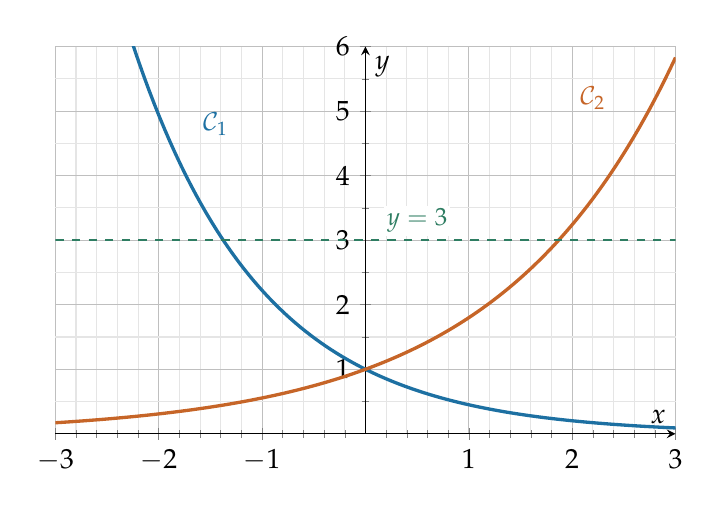
\begin{tikzpicture}
\begin{axis}[width=.78\textwidth,height=6.5cm,axis lines=middle,xmin=-3,xmax=3,ymin=0,ymax=6,
  xtick={-3,...,3},ytick={0,...,6},minor x tick num=4,minor y tick num=1,
  grid=both,major grid style={black!25},minor grid style={black!10},xlabel={$x$},ylabel={$y$}]
\addplot[Blue,very thick,samples=120,domain=-3:3]{0.45^x};
\addplot[Orange,very thick,samples=120,domain=-3:3]{1.8^x};
\addplot[Green,thick,dashed,domain=-3:3]{3};
\node[Blue,font=\small] at (axis cs:-1.45,4.8) {$\mathcal{C}_1$};
\node[Orange,font=\small] at (axis cs:2.2,5.2) {$\mathcal{C}_2$};
\node[Green,font=\small,fill=white,inner sep=1pt] at (axis cs:0.5,3.3) {$y=3$};
\end{axis}
\end{tikzpicture}
\end{center}
\begin{enumerate}
\item Which curve represents the function $f$? Justify your choice.
\item Solve the equation $f(x)=3$ graphically. Using a table of values on the calculator, give an approximate value of the solution to the nearest $0.01$.
\item Determine graphically the set of real numbers $x$ such that $f(x)\geqslant3$, then the set of real numbers $x$ such that $g(x)\geqslant3$.
\end{enumerate}
}{%
\begin{enumerate}
\item $1.8>1$, so $f$ is strictly increasing; $0<0.45<1$, so $g$ is strictly decreasing. The increasing curve $\mathcal{C}_2$ represents $f$ (and $\mathcal{C}_1$ represents $g$). Both curves pass through the point $(0;1)$.
\item The curve $\mathcal{C}_2$ meets the line $y=3$ at a point whose $x$-coordinate reads close to $1.9$. With the calculator: $1.8^{1.86}\approx2.984$ and $1.8^{1.87}\approx3.002$, so the solution lies between $1.86$ and $1.87$; the value $1.87$ gives the image closest to $3$. The solution is $x\approx1.87$.
\item $f(x)\geqslant3$ when $\mathcal{C}_2$ is above the line $y=3$, that is for $x\geqslant1.87$ approximately: $[1.87;+\infty[$ (approximate value of the endpoint).

$g$ is decreasing and $\mathcal{C}_1$ meets the line $y=3$ at an abscissa close to $-1.4$ (calculator: $0.45^{-1.38}\approx3.010$ and $0.45^{-1.37}\approx2.986$, so $x\approx-1.38$). Hence $g(x)\geqslant3$ for $x\leqslant-1.38$ approximately: $]-\infty;-1.38]$ (approximate value of the endpoint).
\end{enumerate}
}{5}

\DefExo{12}{Inequalities with the same base}{%
Solve the following inequalities on $\mathbb{R}$.
\begin{enumerate}[label=\alph*.]
\item $0.7^x\leqslant0.7^{-1}$
\item $2.5^{x+1}>2.5^4$
\item $0.5^x\geqslant0.25$
\end{enumerate}
}{%
\begin{enumerate}[label=\alph*.]
\item $0<0.7<1$: the function $x\mapsto0.7^x$ is strictly decreasing, so it reverses the order. Hence $0.7^x\leqslant0.7^{-1}\iff x\geqslant-1$. Solution set: $[-1;+\infty[$.
\item $2.5>1$: the function $x\mapsto2.5^x$ is strictly increasing, so it preserves the order. Hence $2.5^{x+1}>2.5^4\iff x+1>4\iff x>3$. Solution set: $]3;+\infty[$.
\item $0.25=0.5^2$, so the inequality reads $0.5^x\geqslant0.5^2$. Since $x\mapsto0.5^x$ is strictly decreasing: $x\leqslant2$. Solution set: $]-\infty;2]$.
\end{enumerate}
}{3}

\DefExo{13}{Model with $f(t)=ka^t$ and compute}{%
Just after an injection, the concentration of a drug in a patient's blood is $80$~mg/L. This concentration then decreases by $15\,\%$ every hour. This is an exponential decay.

It is modelled by a function $C$ of the time $t$, in hours, such that $C(t)=ka^t$.
\begin{enumerate}
\item Determine the constants $k$ and $a$.
\item Calculate the concentration after $3$~h~$30$~min, to the nearest $0.1$~mg/L.
\item The doctor plans a new injection as soon as the concentration drops below $50$~mg/L. Is this already the case after $3$~h~$30$~min? Answer in a sentence.
\end{enumerate}
}{%
\begin{enumerate}
\item $C(0)=k\times a^0=k$, and $C(0)=80$, so $k=80$. A $15\,\%$ decrease per hour corresponds to the multiplier $1-\dfrac{15}{100}=0.85$, so $a=0.85$ and $C(t)=80\times0.85^t$.
\item $3$~h~$30$~min $=3.5$~h. $C(3.5)=80\times0.85^{3.5}\approx45.3$~mg/L.
\item $45.3<50$: after $3$~h~$30$~min the concentration has already dropped below $50$~mg/L, so the new injection is due (in fact $C(3)\approx49.1$~mg/L, so the concentration is below this threshold from $3$~h onwards).
\end{enumerate}
}{4}

\DefExo{14}{Average rate of two successive changes}{%
\begin{enumerate}
\item The price of a digital currency rises by $125\,\%$ one year, then falls by $36\,\%$ the following year. What is the average annual rate of change over these two years?
\item The price of a raw material rises by $80\,\%$ one month, then falls by $55\,\%$ the following month. What is the average monthly rate of change?
\item A student claims that, in question 2, the average rate is $\dfrac{80-55}{2}=12.5\,\%$. Explain in a sentence why this is wrong.
\end{enumerate}
}{%
\begin{enumerate}
\item The multipliers are $1+\dfrac{125}{100}=2.25$ and $1-\dfrac{36}{100}=0.64$. The overall multiplier is $2.25\times0.64=1.44$. The average annual multiplier $q$ satisfies $q^2=1.44$, so $q=\sqrt{1.44}=1.2$: an average annual rise of $20\,\%$.
\item The multipliers are $1.8$ and $0.45$; the overall multiplier is $1.8\times0.45=0.81$. The average multiplier is $\sqrt{0.81}=0.9$, that is an average monthly fall of $10\,\%$.
\item Successive changes combine by multiplying the multipliers, not by adding the rates: the $55\,\%$ fall applies to a price that has already risen. Over the two months the price is multiplied by $0.81$ (an overall fall of $19\,\%$), which corresponds to an average fall of $10\,\%$ per month, not a rise of $12.5\,\%$.
\end{enumerate}
}{5}

% Original replacement exercises -- sessions 15 to 30 (chapters 3 and 4).
% Format: \DefExo{session}{target}{statement}{detailed solution}{answer lines}
% Every numerical value has been recomputed by script.

% -----------------------------------------------------------------------------
% Chapter 3 -- Common logarithm function
% -----------------------------------------------------------------------------
\DefExo{15}{Isolate $10^x$, then take the logarithm}{%
Solve the following equations in $\R$. When a solution exists, give its exact value and then its value rounded to the nearest thousandth.
\begin{enumerate}[label=\alph*.]
\item $4\times10^x=9.2$
\item $7\times10^x-1.5=3\times10^x+0.9$
\item $2.5\times10^x+12=6-0.5\times10^x$
\item $10^{x+1}=50$ \quad (you may write $10^{x+1}=10\times10^x$)
\end{enumerate}
}{%
Method: gather the terms in $10^x$ on one side, isolate $10^x$, check that the right-hand side is strictly positive, then use: for $b>0$, $10^x=b \iff x=\log(b)$.
\begin{enumerate}[label=\alph*.]
\item $10^x=\dfrac{9.2}{4}=2.3>0$, so $x=\log(2.3)\approx0.362$.
\item $7\times10^x-3\times10^x=0.9+1.5$, i.e. $4\times10^x=2.4$, so $10^x=0.6>0$ and $x=\log(0.6)\approx-0.222$.
\item $2.5\times10^x+0.5\times10^x=6-12$, i.e. $3\times10^x=-6$, so $10^x=-2$. But $10^x>0$ for every real $x$: the equation has no solution.
\item $10\times10^x=50$, so $10^x=5>0$ and $x=\log(5)\approx0.699$. (Another way: $x+1=\log(50)$, so $x=\log(50)-1=\log(5)$.)
\end{enumerate}
Recommended calculator check: $10^{0.362}\approx2.30$ and $10^{-0.222}\approx0.60$.
}{4}

\DefExo{16}{Sign of a logarithm and comparison}{%
Recall that the function $\log$ is strictly increasing on $]0;+\infty[$ and that $\log(1)=0$.
\begin{enumerate}
\item Without a calculator, give the sign of each of the following numbers, with a justification:
\begin{enumerate}[label=\alph*.]
\item $\log(0.9)$;
\item $\log\!\left(\dfrac{4}{3}\right)$;
\item $\log(CM)$, where $CM$ is the multiplier associated with an increase of $0.2\,\%$.
\end{enumerate}
\item Without a calculator, compare $\log(0.35)$ and $\log(0.53)$.
\end{enumerate}
}{%
\begin{enumerate}
\item For $a>0$: if $a>1$ then $\log(a)>\log(1)=0$; if $0<a<1$ then $\log(a)<0$ (since $\log$ is strictly increasing).
\begin{enumerate}[label=\alph*.]
\item $0<0.9<1$, so $\log(0.9)<0$ (about $-0.046$).
\item $\dfrac43>1$, so $\log\!\left(\dfrac43\right)>0$ (about $0.125$).
\item $CM=1+\dfrac{0.2}{100}=1.002>1$, so $\log(1.002)>0$ (about $0.000\,87$: very close to $0$ but positive).
\end{enumerate}
\item $0<0.35<0.53$ and $\log$ is strictly increasing on $]0;+\infty[$, so $\log(0.35)<\log(0.53)$. Both numbers are negative (arguments less than $1$); the one closer to $0$ is $\log(0.53)$.
\end{enumerate}
}{3}

\DefExo{17}{Condense an expression into one logarithm}{%
Write each of the following numbers in the form $\log(A)$, where $A$ is a strictly positive real number to be given as an integer or a fraction. When possible, give the exact value of the number.
\begin{enumerate}[label=\alph*.]
\item $\log(6)+\log(5)-\log(3)$
\item $2\log(4)-\log(8)$
\item $\log(5)+\log(11)$
\item $2\log(3)-3\log(2)$
\item $\log(40)-\log(8)+2\log(2)$
\end{enumerate}
}{%
We use, for $a,b>0$ and any natural number $n$: $\log(a)+\log(b)=\log(ab)$, $\log(a)-\log(b)=\log\!\left(\dfrac ab\right)$ and $n\log(a)=\log(a^n)$. All the arguments are strictly positive.
\begin{enumerate}[label=\alph*.]
\item $\log(6)+\log(5)-\log(3)=\log\!\left(\dfrac{6\times5}{3}\right)=\log(10)=1$.
\item $2\log(4)-\log(8)=\log(4^2)-\log(8)=\log\!\left(\dfrac{16}{8}\right)=\log(2)$.
\item $\log(5)+\log(11)=\log(55)$.
\item $2\log(3)-3\log(2)=\log(3^2)-\log(2^3)=\log\!\left(\dfrac98\right)$.
\item $\log(40)-\log(8)+2\log(2)=\log\!\left(\dfrac{40\times2^2}{8}\right)=\log(20)$.
\end{enumerate}
Error to point out: $\log(5)+\log(11)$ is not $\log(16)$; a sum of logarithms corresponds to a product of the arguments.
}{4}

\DefExo{18}{Threshold algorithm for a change over time}{%
A delivery company buys a van for $38\,000$~€. Its value is estimated to fall by $15\,\%$ each year. The company will sell the van as soon as its value becomes strictly less than $10\,000$~€.
Let $V$ be the value of the van (in euros) and $N$ the number of years since the purchase.
\begin{center}
\begin{tabular}{|l|}
\hline
$V\leftarrow38\,000$\\
$N\leftarrow0$\\
While $V\ \ldots\ldots\ldots$\\
\hspace*{1.5em}$V\leftarrow\ldots\ldots\ldots$\\
\hspace*{1.5em}$N\leftarrow N+1$\\
End While\\
\hline
\end{tabular}
\end{center}
\begin{enumerate}
\item Complete the algorithm so that, at the end of its execution, the variable $N$ contains the number of years after which the van will be sold.
\item Using the calculator (table of values), run the algorithm and find the value of $N$ obtained. Give the value of the van when it is sold, rounded to the nearest euro.
\item Write this program in Python, run it and compare with the result of question 2.
\end{enumerate}
}{%
\begin{enumerate}
\item A $15\,\%$ decrease corresponds to the multiplier $1-0.15=0.85$. We repeat as long as the value has not yet fallen below the threshold: “While $V\geqslant10\,000$” and “$V\leftarrow0.85\times V$”.
\item Successive values rounded to the nearest euro: $N=6$: $14\,332$~€; $N=7$: $12\,182$~€; $N=8$: $10\,355$~€; $N=9$: $8\,801$~€.
Since $38\,000\times0.85^8\approx10\,355\geqslant10\,000$ and $38\,000\times0.85^9\approx8\,801<10\,000$, the loop stops with $N=9$: the van will be sold after $9$ years, for a value of about $8\,801$~€.
\item A possible program:\\
\texttt{V = 38000}\\
\texttt{N = 0}\\
\texttt{while V >= 10000:}\\
\hspace*{2em}\texttt{V = 0.85 * V}\\
\hspace*{2em}\texttt{N = N + 1}\\
\texttt{print(N, V)}\\
The program displays $9$ and about $8801.44$, which confirms question 2. Stress the decimal point in Python and the indentation of the loop block.
\end{enumerate}
}{5}

\DefExo{19}{Doubling time and overtaking}{%
An online shop A received $2\,500$ orders in January 2026. This number is assumed to increase by $7\,\%$ per month. Let $a_n$ be the number of orders $n$ months after January 2026.
\begin{enumerate}
\item
\begin{enumerate}[label=\alph*.]
\item Express $a_n$ in terms of $n$.
\item After how many months will the monthly number of orders have doubled?
\item After how many months will it have quadrupled? Is this result twice the previous one? Explain.
\end{enumerate}
\item A competing shop B received $4\,000$ orders in January 2026, with an increase of $3\,\%$ per month. From how many months on will shop A have more monthly orders than shop B? In which month will this happen?
\end{enumerate}
}{%
\begin{enumerate}
\item
\begin{enumerate}[label=\alph*.]
\item An increase of $7\,\%$ corresponds to the multiplier $1.07$: $a_n=2\,500\times1.07^n$.
\item $a_n\geqslant5\,000\iff1.07^n\geqslant2\iff n\log(1.07)\geqslant\log(2)\iff n\geqslant\dfrac{\log(2)}{\log(1.07)}$, because $\log(1.07)>0$ (the inequality keeps its direction). Now $\dfrac{\log 2}{\log 1.07}\approx10.24$: $11$ months are needed. Check: $1.07^{10}\approx1.967<2$ and $1.07^{11}\approx2.105\geqslant2$.
\item $1.07^n\geqslant4\iff n\geqslant\dfrac{\log(4)}{\log(1.07)}\approx20.49$: $21$ months are needed ($1.07^{20}\approx3.870$ and $1.07^{21}\approx4.141$). Since $\log(4)=2\log(2)$, the exact threshold is indeed doubled ($20.49=2\times10.24$), but rounding up to the next integer happens only once: $21$, not $2\times11=22$.
\end{enumerate}
\item We look for $n$ such that $2\,500\times1.07^n>4\,000\times1.03^n$. Dividing by $2\,500\times1.03^n>0$: $\left(\dfrac{1.07}{1.03}\right)^n>1.6$. Since $\dfrac{1.07}{1.03}>1$, its logarithm is positive and $n>\dfrac{\log(1.6)}{\log(1.07/1.03)}\approx12.34$. Hence $n=13$: check $a_{12}\approx5\,630<5\,703$ and $a_{13}\approx6\,025>5\,874$. Shop A will overtake shop B in February 2027 ($13$ months after January 2026).
\end{enumerate}
}{5}

\DefExo{20}{Finding a rate: equation $x^n=b$}{%
The retail price of a solar panel model went from $420$~€ in March 2021 to $260$~€ in September 2025, a period of $4$ years and $6$ months. The price is assumed to have changed at a constant annual rate $t$.
\begin{enumerate}
\item Justify that $(1+t)^{4.5}=\dfrac{260}{420}$.
\item Deduce $t$, rounded to $0.1\,\%$. Interpret the sign of the result.
\item A second model costs $395$~€ today. If its price changes at the same annual rate, what will its price be in $2$ years and $3$ months? Round to the nearest euro.
\item The manufacturer of this second model would rather reach a price of $300$~€ in $2$ years and $3$ months. What constant annual rate should it apply? Round to $0.1\,\%$.
\end{enumerate}
}{%
\begin{enumerate}
\item Over $4.5$ years, the price is multiplied by $(1+t)^{4.5}$, so $420(1+t)^{4.5}=260$, i.e. $(1+t)^{4.5}=\dfrac{260}{420}\approx0.619$.
\item $1+t>0$, so $1+t=\left(\dfrac{260}{420}\right)^{1/4.5}\approx0.8989$, hence $t\approx-0.101$, i.e. $t\approx-10.1\,\%$. The rate is negative: the price fell on average by about $10.1\,\%$ per year. Check: $420\times0.8989^{4.5}\approx260$.
\item $2$ years and $3$ months $=2.25$ years. Price: $395(1+t)^{2.25}$. Keeping the exact value of $1+t$ in memory: $395\times\left(\dfrac{260}{420}\right)^{2.25/4.5}=395\times\left(\dfrac{260}{420}\right)^{0.5}\approx395\times0.7868\approx310.78$. The price would be about $311$~€.
\item We solve $395(1+t')^{2.25}=300$, i.e. $(1+t')^{2.25}=\dfrac{300}{395}\approx0.7595$, so $1+t'=\left(\dfrac{300}{395}\right)^{1/2.25}\approx0.8849$ and $t'\approx-11.5\,\%$. A decrease of about $11.5\,\%$ per year would be needed.
\end{enumerate}
Remark: using a value of $t$ rounded too early slightly changes the results (for example $395\times0.899^{2.25}\approx310.85$); keep the value in memory.
}{4}

\DefExo{21}{Using a formula $\log(N)/\log(2)$}{%
In a laboratory, a cell culture grows by successive divisions: at each generation, the number of cells doubles. When the number of cells goes from $N_0$ to $N$, the number of generations that have elapsed is
\[
g=\frac{\log\!\left(\dfrac{N}{N_0}\right)}{\log(2)}.
\]
For example, going from $1$ to $8$ cells corresponds to $g=\dfrac{\log(8)}{\log(2)}=3$ generations.
\begin{enumerate}
\item A culture goes from $1\,000$ to $64\,000$ cells. How many generations have elapsed?
\item Another culture goes from $500$ to $128\,000$ cells. Same question.
\item A culture of $1\,000$ cells develops for $9.5$ generations. About how many cells does it contain?
\item Starting from a single cell, how many cells are obtained after $20$ generations?
\item A laboratory starts from $1\,000$ cells and wants to obtain $1\,000\,000\,000$. How many generations are needed? Given that one generation lasts $30$ minutes, how much time should be planned?
\end{enumerate}
}{%
\begin{enumerate}
\item $\dfrac{N}{N_0}=64=2^6$, so $g=\dfrac{\log(2^6)}{\log(2)}=\dfrac{6\log(2)}{\log(2)}=6$ generations.
\item $\dfrac{N}{N_0}=\dfrac{128\,000}{500}=256=2^8$, so $g=8$ generations.
\item $g=9.5$ gives $\log\!\left(\dfrac{N}{1\,000}\right)=9.5\log(2)$, so $\dfrac{N}{1\,000}=10^{9.5\log(2)}=2^{9.5}\approx724.08$. Thus $N\approx724\,000$ cells.
\item $N=2^{20}=1\,048\,576$ cells, i.e. about one million.
\item $\dfrac{N}{N_0}=10^6$, so $g=\dfrac{\log(10^6)}{\log(2)}=\dfrac{6}{\log(2)}\approx19.93$: $20$ complete generations are needed. Time: $20\times30=600$ minutes, i.e. about $10$ hours.
\end{enumerate}
}{5}

\DefExo{22}{Number of digits of an integer}{%
We look for a method to find the number of digits of a natural number $N\geqslant1$ without writing it out in full. The integer part of a real number $y\geqslant0$ is the greatest integer less than or equal to $y$; it is denoted $E(y)$.
\begin{enumerate}
\item Let $N=4\,718$.
\begin{enumerate}[label=\alph*.]
\item Bound $N$ between two consecutive powers of $10$. Deduce bounds for $\log(N)$ between two consecutive integers.
\item Compare $E(\log N)$ with the number of digits of $N$.
\end{enumerate}
\item An integer $N$ is written with $15$ digits.
\begin{enumerate}[label=\alph*.]
\item Bound $N$ between two consecutive powers of $10$, then $\log(N)$ between two consecutive integers.
\item What is $E(\log N)$?
\end{enumerate}
\item State a rule giving the number of digits of $N$ from $\log(N)$. Test it on $N=1\,000$.
\item Use this rule to find the number of digits of: a. $3^{100}$; b. $2^{64}$; c. $365\times10^{15}$.
\item A password is made of $12$ characters, each chosen from $62$ symbols ($26$ lower-case letters, $26$ upper-case letters, $10$ digits). There are $62^{12}$ possible passwords. How many digits does this number have?
\end{enumerate}
}{%
\begin{enumerate}
\item
\begin{enumerate}[label=\alph*.]
\item $10^3\leqslant4\,718<10^4$. Since $\log$ is strictly increasing, $3\leqslant\log(4\,718)<4$ (we find $\log(4\,718)\approx3.674$).
\item $E(\log N)=3$ and $N$ has $4$ digits: number of digits $=E(\log N)+1$.
\end{enumerate}
\item
\begin{enumerate}[label=\alph*.]
\item The smallest $15$-digit integer is $10^{14}$ and the smallest $16$-digit integer is $10^{15}$: $10^{14}\leqslant N<10^{15}$, so $14\leqslant\log(N)<15$.
\item $E(\log N)=14$, and $14+1=15$ digits.
\end{enumerate}
\item If $N$ has $k$ digits, $10^{k-1}\leqslant N<10^k$, so $k-1\leqslant\log(N)<k$: $E(\log N)=k-1$. Rule: \emph{the number of digits of $N$ is $E(\log N)+1$}. For $N=1\,000$: $\log(1\,000)=3$, $E(3)+1=4$ digits, which is correct.
\item a. $\log(3^{100})=100\log(3)\approx47.71$: $47+1=48$ digits.\\
b. $\log(2^{64})=64\log(2)\approx19.27$: $20$ digits (indeed $2^{64}=18\,446\,744\,073\,709\,551\,616$).\\
c. $\log(365\times10^{15})=\log(365)+15\approx17.56$: $18$ digits.
\item $\log(62^{12})=12\log(62)\approx21.51$: $62^{12}$ is written with $22$ digits (about $3.2\times10^{21}$ passwords).
\end{enumerate}
}{6}

% -----------------------------------------------------------------------------
% Chapter 4 -- Reciprocal function
% -----------------------------------------------------------------------------
\DefExo{23}{Table of values and plotting hyperbolas}{%
Consider the functions $f$ and $g$ defined on $\R^{*}=\R\setminus\{0\}$ by
$f(x)=-\dfrac{2}{x}$ and $g(x)=1+\dfrac{3}{x}$.
\begin{enumerate}
\item Explain why $0$ does not belong to the domain of these functions.
\item Complete the table of values (values rounded to the nearest hundredth if necessary).
\begin{center}\small
\begin{tabular}{|c|*{10}{c|}}
\hline
$x$ & $-4$ & $-3$ & $-2$ & $-1$ & $-0.5$ & $0.5$ & $1$ & $2$ & $3$ & $4$\\
\hline
$f(x)$ & & & & & & & & & & \\
\hline
$g(x)$ & & & & & & & & & & \\
\hline
\end{tabular}
\end{center}
\item Plot the points and draw the curves $\mathcal{C}_f$ and $\mathcal{C}_g$ on the grid below.
\begin{center}
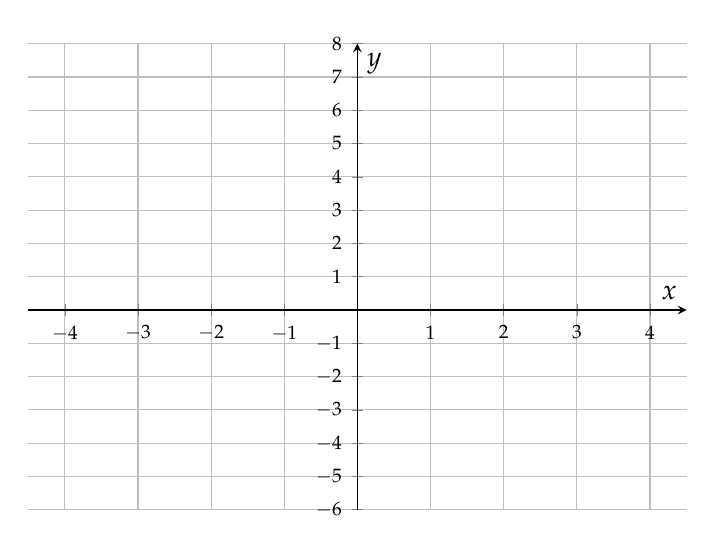
\begin{tikzpicture}
\begin{axis}[width=.82\linewidth,height=7.5cm,axis lines=middle,xmin=-4.5,xmax=4.5,ymin=-6,ymax=8,
  xtick={-4,...,4},ytick={-6,...,8},grid=major,xlabel={$x$},ylabel={$y$},tick label style={font=\scriptsize}]
\end{axis}
\end{tikzpicture}
\end{center}
\item Show that, for every non-zero real $x$, $f(-x)=-f(x)$. Which symmetry of $\mathcal{C}_f$ does this express? For each curve, give the lines it gets closer and closer to (asymptotes).
\end{enumerate}
}{%
\begin{enumerate}
\item Computing $\dfrac2x$ or $\dfrac3x$ requires dividing by $x$; division by $0$ is impossible. The domain is $\R^{*}=]-\infty;0[\cup]0;+\infty[$.
\item
\begin{center}\small
\begin{tabular}{|c|*{10}{c|}}
\hline
$x$ & $-4$ & $-3$ & $-2$ & $-1$ & $-0.5$ & $0.5$ & $1$ & $2$ & $3$ & $4$\\
\hline
$f(x)$ & $0.5$ & $0.67$ & $1$ & $2$ & $4$ & $-4$ & $-2$ & $-1$ & $-0.67$ & $-0.5$\\
\hline
$g(x)$ & $0.25$ & $0$ & $-0.5$ & $-2$ & $-5$ & $7$ & $4$ & $2.5$ & $2$ & $1.75$\\
\hline
\end{tabular}
\end{center}
\item
\begin{center}
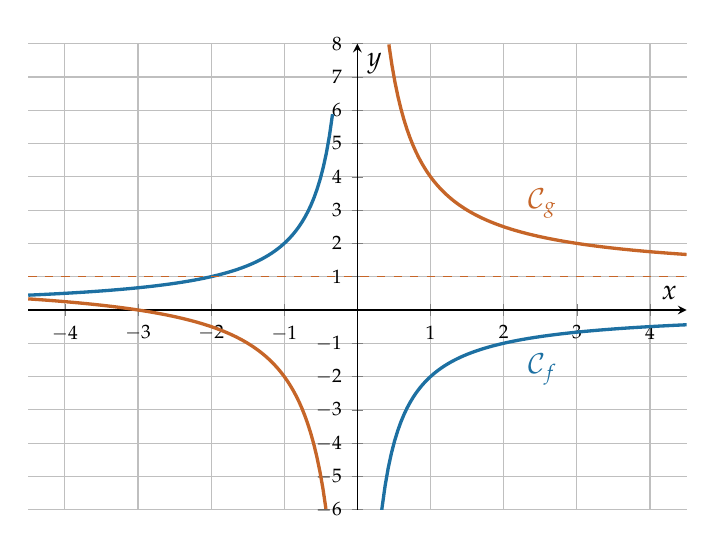
\begin{tikzpicture}
\begin{axis}[width=.82\linewidth,height=7.5cm,axis lines=middle,xmin=-4.5,xmax=4.5,ymin=-6,ymax=8,
  xtick={-4,...,4},ytick={-6,...,8},grid=major,xlabel={$x$},ylabel={$y$},tick label style={font=\scriptsize}]
\addplot[Blue,very thick,samples=100,domain=-4.5:-0.34]{-2/x};
\addplot[Blue,very thick,samples=100,domain=0.25:4.5]{-2/x};
\addplot[Orange,very thick,samples=100,domain=-4.5:-0.43]{1+3/x};
\addplot[Orange,very thick,samples=100,domain=0.43:4.5]{1+3/x};
\addplot[Orange,dashed] coordinates {(-4.5,1)(4.5,1)};
\node[Blue,anchor=west] at (axis cs:2.2,-1.8) {$\mathcal{C}_f$};
\node[Orange,anchor=west] at (axis cs:2.2,3.2) {$\mathcal{C}_g$};
\end{axis}
\end{tikzpicture}
\end{center}
\item $f(-x)=-\dfrac{2}{-x}=\dfrac2x=-f(x)$. The points with coordinates $(x;f(x))$ and $(-x;-f(x))$ are symmetric about the origin: $\mathcal{C}_f$ is symmetric about the origin $O$. Asymptotes: for $\mathcal{C}_f$, the lines with equations $x=0$ and $y=0$; for $\mathcal{C}_g$, the lines with equations $x=0$ and $y=1$ (the curve of $g$ is symmetric about the point $(0;1)$, since $g(-x)+g(x)=2$).
\end{enumerate}
}{5}

\DefExo{24}{End behaviour and asymptotes}{%
Let $h$ be the function defined on $\R^{*}$ by $h(x)=-1+\dfrac{5}{x}$.
\begin{enumerate}
\item Compute $h(x)$ for $x\in\{-10\,000;-1\,000;-100;100;1\,000;10\,000\}$. What can be conjectured about $h(x)$ when $x$ becomes very large in absolute value? Which asymptote can be deduced?
\item Compute $h(x)$ for $x\in\{-0.1;-0.01;-0.001;0.001;0.01;0.1\}$. Describe the behaviour of $h(x)$ when $x$ gets close to $0$, first through negative values, then through positive values. Which asymptote can be deduced?
\item Compute $h(-5)$, $h(-1)$, $h(1)$ and $h(5)$, then sketch the curve of $h$ and its asymptotes on the grid below.
\begin{center}
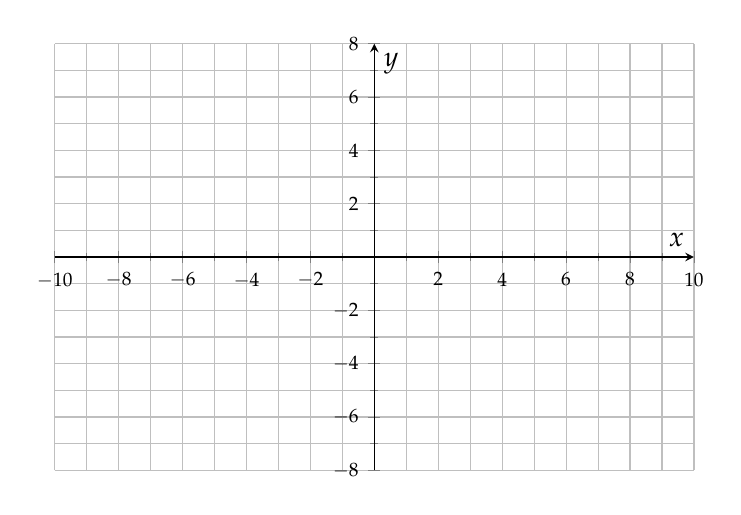
\begin{tikzpicture}
\begin{axis}[width=.8\linewidth,height=7cm,axis lines=middle,xmin=-10,xmax=10,ymin=-8,ymax=8,
  xtick={-10,-8,...,10},ytick={-8,-6,...,8},minor tick num=1,grid=both,xlabel={$x$},ylabel={$y$},tick label style={font=\scriptsize}]
\end{axis}
\end{tikzpicture}
\end{center}
\item Application. A training organisation rents a room for $450$~€ per day and spends $12$~€ on meals per participant. For $x$ participants ($x\geqslant1$), the average cost per participant is $c(x)=12+\dfrac{450}{x}$ (in euros).
\begin{enumerate}[label=\alph*.]
\item Compute $c(10)$, $c(50)$ and $c(150)$.
\item Which value does the average cost get closer to when the number of participants becomes very large? Can it fall below $12$~€? Justify.
\end{enumerate}
\end{enumerate}
}{%
\begin{enumerate}
\item $h(-10\,000)=-1.000\,5$; $h(-1\,000)=-1.005$; $h(-100)=-1.05$; $h(100)=-0.95$; $h(1\,000)=-0.995$; $h(10\,000)=-0.999\,5$. When $|x|$ becomes very large, $\dfrac5x$ gets close to $0$, so $h(x)$ gets close to $-1$ (from below at $-\infty$, from above at $+\infty$). The line with equation $y=-1$ is a horizontal asymptote.
\item $h(-0.1)=-51$; $h(-0.01)=-501$; $h(-0.001)=-5\,001$; $h(0.001)=4\,999$; $h(0.01)=499$; $h(0.1)=49$. When $x$ gets close to $0$ through negative values, $h(x)$ is negative and as large as we like in absolute value ($h(x)\to-\infty$); through positive values, $h(x)\to+\infty$. The line with equation $x=0$ is a vertical asymptote.
\item $h(-5)=-2$, $h(-1)=-6$, $h(1)=4$, $h(5)=0$.
\begin{center}
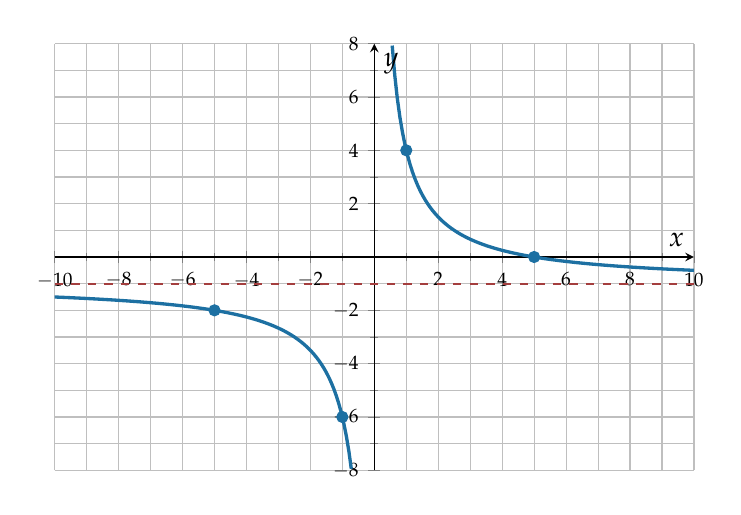
\begin{tikzpicture}
\begin{axis}[width=.8\linewidth,height=7cm,axis lines=middle,xmin=-10,xmax=10,ymin=-8,ymax=8,
  xtick={-10,-8,...,10},ytick={-8,-6,...,8},minor tick num=1,grid=both,xlabel={$x$},ylabel={$y$},tick label style={font=\scriptsize}]
\addplot[Blue,very thick,samples=120,domain=-10:-0.72]{-1+5/x};
\addplot[Blue,very thick,samples=120,domain=0.56:10]{-1+5/x};
\addplot[Red,dashed,thick] coordinates {(-10,-1)(10,-1)};
\addplot[only marks,mark=*,Blue] coordinates {(-5,-2)(-1,-6)(1,4)(5,0)};
\end{axis}
\end{tikzpicture}
\end{center}
\item
\begin{enumerate}[label=\alph*.]
\item $c(10)=12+45=57$~€; $c(50)=12+9=21$~€; $c(150)=12+3=15$~€.
\item When $x$ becomes very large, $\dfrac{450}{x}$ gets close to $0$: the average cost gets close to $12$~€ (asymptote $y=12$). Since $\dfrac{450}{x}>0$ for $x>0$, we always have $c(x)>12$: the average cost never falls below $12$~€, as the fixed cost of the room is shared among the participants without disappearing.
\end{enumerate}
\end{enumerate}
}{5}

\DefExo{25}{Differentiate a polynomial plus $k/x$}{%
Compute the derivative of each of the following functions, defined on $\R^{*}$.
\begin{enumerate}[label=\alph*.]
\item $f(x)=5x+2-\dfrac{3}{x}$
\item $g(x)=-4x+7+\dfrac{6}{x}$
\item $h(x)=2x^3-5x^2+\dfrac{1}{x}$
\item $k(x)=\dfrac12x^2+4x-\dfrac{8}{x}$
\item $p(x)=\dfrac{x^2+2}{x}$ \quad (first write $p(x)$ in the form $x+\dfrac{a}{x}$, then give $p'(x)$ as a single quotient)
\end{enumerate}
}{%
We use: $(ax^n)'=nax^{n-1}$, the derivative of a constant is zero and, for $x\neq0$, $\left(\dfrac{k}{x}\right)'=k\times\left(-\dfrac1{x^2}\right)=-\dfrac{k}{x^2}$.
\begin{enumerate}[label=\alph*.]
\item $f'(x)=5-\left(-\dfrac{3}{x^2}\right)=5+\dfrac{3}{x^2}$.
\item $g'(x)=-4-\dfrac{6}{x^2}$.
\item $h'(x)=6x^2-10x-\dfrac{1}{x^2}$.
\item $k'(x)=x+4+\dfrac{8}{x^2}$.
\item $p(x)=\dfrac{x^2}{x}+\dfrac{2}{x}=x+\dfrac2x$, so $p'(x)=1-\dfrac2{x^2}=\dfrac{x^2-2}{x^2}$.
\end{enumerate}
Common error: writing $\left(\dfrac{3}{x}\right)'=\dfrac{3}{x^2}$, forgetting the “$-$” sign.
}{5}

\DefExo{26}{Factorised derivative, sign and variations}{%
Let $f$ be the function defined on $\R^{*}$ by $f(x)=9x-2+\dfrac{4}{x}$.
\begin{enumerate}
\item Show that, for every non-zero real $x$, $f'(x)=\dfrac{(3x-2)(3x+2)}{x^2}$.
\item Study the sign of $f'(x)$ on $\R^{*}$ using a sign table.
\item Deduce the table of variations of $f$, including the values of $f\!\left(-\dfrac23\right)$ and $f\!\left(\dfrac23\right)$.
\item Compare $f\!\left(-\dfrac23\right)$ and $f\!\left(\dfrac23\right)$. Can a local maximum be less than a local minimum? Explain using the table.
\end{enumerate}
}{%
\begin{enumerate}
\item $f'(x)=9-\dfrac{4}{x^2}=\dfrac{9x^2-4}{x^2}=\dfrac{(3x-2)(3x+2)}{x^2}$ (identity $a^2-b^2=(a-b)(a+b)$ with $a=3x$, $b=2$).
\item $x^2>0$ for $x\neq0$: the sign of $f'(x)$ is that of $(3x-2)(3x+2)$. $3x+2=0\iff x=-\dfrac23$; $3x-2=0\iff x=\dfrac23$.
\[
\begin{array}{|c|ccccccccc|}
\hline
x & -\infty & & -\frac23 & & 0 & & \frac23 & & +\infty\\ \hline
3x+2 & & - & 0 & + & \| & + & & + & \\
3x-2 & & - & & - & \| & - & 0 & + & \\
x^2 & & + & & + & 0 & + & & + & \\ \hline
f'(x) & & + & 0 & - & \| & - & 0 & + & \\ \hline
\end{array}
\]
\item $f\!\left(-\dfrac23\right)=-6-2-6=-14$ and $f\!\left(\dfrac23\right)=6-2+6=10$.
\[
\begin{array}{|c|ccccccccc|}
\hline
x & -\infty & & -\frac23 & & 0 & & \frac23 & & +\infty\\ \hline
f(x) & & \nearrow & -14 & \searrow & \| & \searrow & 10 & \nearrow & \\ \hline
\end{array}
\]
$f$ is increasing on $\left]-\infty;-\dfrac23\right]$, decreasing on $\left[-\dfrac23;0\right[$ and on $\left]0;\dfrac23\right]$, increasing on $\left[\dfrac23;+\infty\right[$.
\item $-14<10$: the local maximum (reached at $-\dfrac23$, on $]-\infty;0[$) is less than the local minimum (reached at $\dfrac23$, on $]0;+\infty[$). This is not a contradiction: they are local extrema on two intervals separated by the forbidden value $0$, where the curve “jumps” (vertical asymptote).
\end{enumerate}
}{4}

\DefExo{27}{Always-positive derivative and sign of a quotient}{%
Let $h$ be the function defined on $\R^{*}$ by $h(x)=2x-3-\dfrac{5}{x}$.
\begin{enumerate}
\item Show that, for every non-zero real $x$, $h'(x)=\dfrac{2x^2+5}{x^2}$.
\item Study the sign of $h'(x)$ and deduce the variations of $h$.
\item Compute $h(-1)$ and $h(1)$. Can we say that “$h$ is increasing on $\R^{*}$”? Explain.
\item Show that, for every non-zero real $x$, $h(x)=\dfrac{(2x-5)(x+1)}{x}$. Draw the sign table of $h(x)$, then solve the inequality $h(x)\geqslant0$.
\end{enumerate}
}{%
\begin{enumerate}
\item $h'(x)=2-\left(-\dfrac{5}{x^2}\right)=2+\dfrac{5}{x^2}=\dfrac{2x^2+5}{x^2}$.
\item For $x\neq0$: $2x^2+5\geqslant5>0$ and $x^2>0$, so $h'(x)>0$. The function $h$ is strictly increasing on $]-\infty;0[$ and strictly increasing on $]0;+\infty[$.
\[
\begin{array}{|c|ccccc|}
\hline
x & -\infty & & 0 & & +\infty\\ \hline
h'(x) & & + & \| & + & \\ \hline
h(x) & & \nearrow & \| & \nearrow & \\ \hline
\end{array}
\]
\item $h(-1)=-2-3+5=0$ and $h(1)=2-3-5=-6$. We have $-1<1$ but $h(-1)>h(1)$: $h$ is not increasing on the whole of $\R^{*}$. It is increasing on each of the two intervals, separately.
\item $\dfrac{(2x-5)(x+1)}{x}=\dfrac{2x^2-3x-5}{x}=2x-3-\dfrac5x=h(x)$. Critical values: $-1$, $0$ (forbidden value) and $\dfrac52$.
\[
\begin{array}{|c|ccccccccc|}
\hline
x & -\infty & & -1 & & 0 & & \frac52 & & +\infty\\ \hline
2x-5 & & - & & - & & - & 0 & + & \\
x+1 & & - & 0 & + & & + & & + & \\
x & & - & & - & 0 & + & & + & \\ \hline
h(x) & & - & 0 & + & \| & - & 0 & + & \\ \hline
\end{array}
\]
The solution set of $h(x)\geqslant0$ is $[-1;0[\cup\left[\dfrac52;+\infty\right[$ ($0$ is excluded as a forbidden value). Check: $h(-0.5)=6>0$, $h(1)=-6<0$, $h(3)=\dfrac43>0$.
\end{enumerate}
}{5}

\DefExo{28}{Derivative and variations of the reciprocal function}{%
Let $f$ be the reciprocal function, defined on $\R^{*}$ by $f(x)=\dfrac1x$.
\begin{enumerate}
\item Let $h$ be a non-zero real number, with $h\neq-2$. Show that the rate of change of $f$ between $2$ and $2+h$ is
$\dfrac{f(2+h)-f(2)}{h}=-\dfrac{1}{2(2+h)}$. Letting $h$ tend to $0$, deduce $f'(2)$.
\item We admit that, for every non-zero real $x$, $f'(x)=-\dfrac1{x^2}$. Check consistency with question 1, then compute $f'(-1)$ and $f'(0.5)$.
\item Study the sign of $f'(x)$ and draw the table of variations of $f$.
\item A student notices that $-2<3$ and $f(-2)<f(3)$, and claims that this contradicts the fact that $f$ is decreasing. What should we answer?
\end{enumerate}
}{%
\begin{enumerate}
\item $f(2+h)-f(2)=\dfrac1{2+h}-\dfrac12=\dfrac{2-(2+h)}{2(2+h)}=\dfrac{-h}{2(2+h)}$. Dividing by $h\neq0$: $\dfrac{f(2+h)-f(2)}{h}=-\dfrac1{2(2+h)}$. When $h$ tends to $0$, this rate tends to $-\dfrac1{2\times2}=-\dfrac14$: $f'(2)=-\dfrac14$.
\item $-\dfrac1{2^2}=-\dfrac14$: consistent. $f'(-1)=-\dfrac1{(-1)^2}=-1$ and $f'(0.5)=-\dfrac1{0.25}=-4$ (slopes of the tangents at these points).
\item For $x\neq0$, $x^2>0$, so $f'(x)=-\dfrac1{x^2}<0$.
\[
\begin{array}{|c|ccccc|}
\hline
x & -\infty & & 0 & & +\infty\\ \hline
f'(x) & & - & \| & - & \\ \hline
f(x) & & \searrow & \| & \searrow & \\ \hline
\end{array}
\]
$f$ is strictly decreasing on $]-\infty;0[$ and strictly decreasing on $]0;+\infty[$.
\item $f(-2)=-0.5$ and $f(3)\approx0.33$: indeed $f(-2)<f(3)$. There is no contradiction: $-2$ and $3$ are not in the same interval. The reciprocal function is decreasing on each interval separately, not on the whole of $\R^{*}$; images can be compared using the direction of variation only for two real numbers in the same interval.
\end{enumerate}
}{4}

\DefExo{29}{Reading an average cost from a graph}{%
A company assembles between $10$ and $70$ electric bicycles per month. For $x$ bicycles assembled, let $C(x)$ be the average unit production cost, in euros. The curve of the function $C$ on $[10;70]$ is given below.
\begin{center}
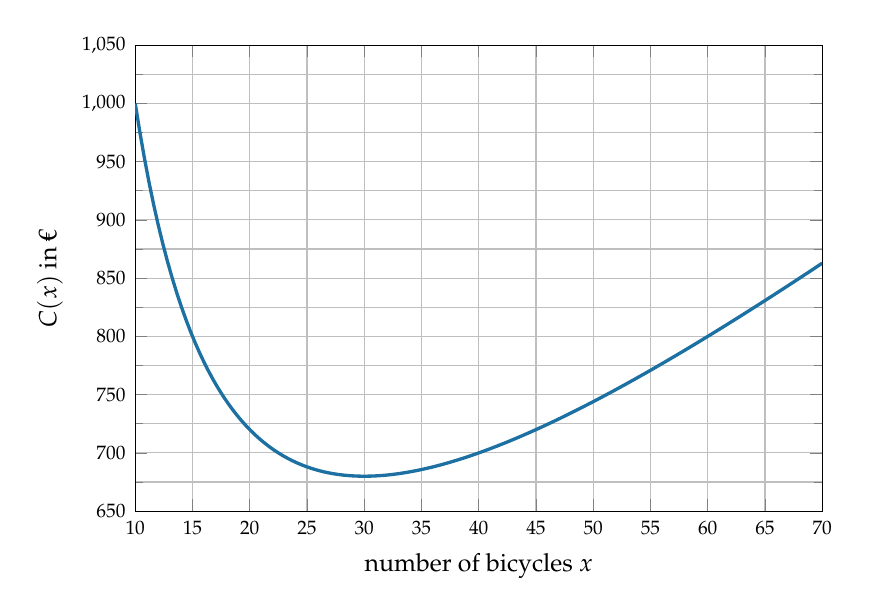
\begin{tikzpicture}
\begin{axis}[width=.85\linewidth,height=7.5cm,xmin=10,xmax=70,ymin=650,ymax=1050,
  xtick={10,15,...,70},ytick={650,700,...,1050},minor y tick num=1,grid=both,
  xlabel={number of bicycles $x$},ylabel={$C(x)$ in €},tick label style={font=\scriptsize},label style={font=\small}]
\addplot[Blue,very thick,samples=150,domain=10:70]{8*x+200+7200/x};
\end{axis}
\end{tikzpicture}
\end{center}
\begin{enumerate}
\item Read the average unit cost when the company assembles $15$ bicycles, then $50$ bicycles.
\item For which production levels is the average unit cost equal to $800$~€?
\item What is the minimum average unit cost? For which production level is it reached?
\item We admit that $C(x)=8x+200+\dfrac{7\,200}{x}$. Compute $C'(x)$, check that $C'(x)=\dfrac{8(x-30)(x+30)}{x^2}$ and confirm the answer to question 3 by calculation.
\end{enumerate}
}{%
Require reading lines (dotted) and units; a graphical reading is approximate.
\begin{enumerate}
\item We read $C(15)\approx800$~€ and $C(50)\approx745$~€ (exact value with the formula of question 4: $744$~€).
\item Draw the line with equation $y=800$: it meets the curve at the points with abscissas $15$ and $60$. The average cost is $800$~€ for $15$ or $60$ bicycles.
\item The lowest point of the curve has coordinates about $(30;680)$: minimum cost of about $680$~€ per bicycle, for $30$ bicycles per month.
\item $C'(x)=8-\dfrac{7\,200}{x^2}=\dfrac{8x^2-7\,200}{x^2}=\dfrac{8(x^2-900)}{x^2}=\dfrac{8(x-30)(x+30)}{x^2}$. On $[10;70]$, $x+30>0$ and $x^2>0$: $C'(x)$ has the sign of $x-30$, negative on $[10;30[$ and positive on $]30;70]$. $C$ is decreasing on $[10;30]$ then increasing on $[30;70]$; its minimum is $C(30)=240+200+240=680$~€. Checks: $C(15)=120+200+480=800$ and $C(60)=480+200+120=800$.
\end{enumerate}
}{5}

\DefExo{30}{Minimising an average cost with the derivative}{%
A composting site produces $x$ tonnes of compost each week, with $x\in[2;25]$. The total weekly production cost, in euros, is modelled by $C(x)=2x^2+40x+288$.
Let $f$ be the function giving the average production cost of one tonne: $f(x)=\dfrac{C(x)}{x}$.
\begin{enumerate}
\item Show that, for every $x\in[2;25]$, $f(x)=2x+40+\dfrac{288}{x}$.
\item Compute $f'(x)$ and show that, for every $x\in[2;25]$, $f'(x)=\dfrac{2(x-12)(x+12)}{x^2}$.
\item Study the sign of $f'(x)$ on $[2;25]$ and draw the table of variations of $f$ (including the values at the endpoints).
\item What is the minimum average cost of one tonne of compost? For which weekly production is it reached? What is the total cost of the week then?
\end{enumerate}
}{%
\begin{enumerate}
\item For $x\in[2;25]$, $x\neq0$: $f(x)=\dfrac{2x^2}{x}+\dfrac{40x}{x}+\dfrac{288}{x}=2x+40+\dfrac{288}{x}$.
\item $f'(x)=2-\dfrac{288}{x^2}=\dfrac{2x^2-288}{x^2}=\dfrac{2(x^2-144)}{x^2}=\dfrac{2(x-12)(x+12)}{x^2}$.
\item On $[2;25]$: $2>0$, $x+12>0$ and $x^2>0$, so $f'(x)$ has the sign of $x-12$: $f'(x)<0$ on $[2;12[$, $f'(12)=0$, $f'(x)>0$ on $]12;25]$.
$f(2)=4+40+144=188$; $f(12)=24+40+24=88$; $f(25)=50+40+11.52=101.52$.
\[
\begin{array}{|c|ccccc|}
\hline
x & 2 & & 12 & & 25\\ \hline
f'(x) & & - & 0 & + & \\ \hline
f(x) & 188 & \searrow & 88 & \nearrow & 101.52\\ \hline
\end{array}
\]
\item The minimum average cost is $88$~€ per tonne, reached for a production of $12$ tonnes per week. The total cost is then $C(12)=288+480+288=1\,056$~€ (check: $12\times88=1\,056$).
\end{enumerate}
}{4}

% Original exercises for sessions 31 to 46 (chapters 5 and 6).
% One command per session: \DefExo{session}{target}{statement}{solution}{lines}.

% -----------------------------------------------------------------------------
% Chapter 5 -- Two-variable quantitative statistics
% -----------------------------------------------------------------------------
\DefExo{31}{Building a scatter plot}{%
Over six months, a convenience store compares the gap $x_i$ between the month's average temperature and the seasonal norm (in °C) with the change $y_i$ in its cold-drink sales compared with the same month of the previous year (in hundreds of bottles).
\[
\begin{array}{c|rrrrrr}
\text{Temperature gap }x_i\text{ (°C)}&-4&-1&0&2&5&7\\\hline
\text{Change in sales }y_i\text{ (hundreds)}&-3&-2&0&2&4&5
\end{array}
\]
\begin{enumerate}
\item State the variable placed on the horizontal axis, the one placed on the vertical axis, and their units.
\item Choose suitable scales, then plot the scatter plot of the points $M_i(x_i;y_i)$ on a coordinate grid.
\item Calculate the coordinates of the mean point $G$ of the scatter plot and plot it.
\item Describe the shape of the scatter plot in one sentence.
\end{enumerate}
}{%
\begin{enumerate}
\item Horizontal axis: the temperature gap $x$, in °C; vertical axis: the change in sales $y$, in hundreds of bottles. Both variables take negative values: the axes must cross inside the graph.
\item One can take $1$~cm for $1$~°C (from $-5$ to $8$) and $1$~cm for one hundred bottles (from $-4$ to $6$). Plot the six points $(-4;-3)$, $(-1;-2)$, $(0;0)$, $(2;2)$, $(5;4)$ and $(7;5)$, without joining them.
\begin{center}
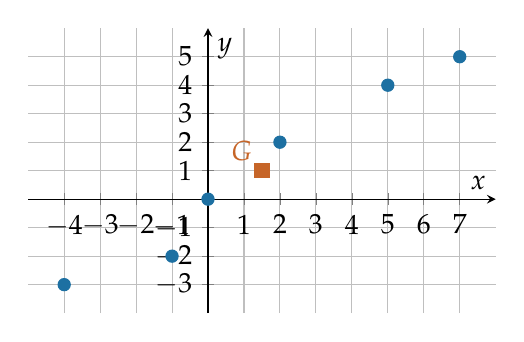
\begin{tikzpicture}
\begin{axis}[width=.62\textwidth,height=5.2cm,axis lines=middle,xmin=-5,xmax=8,ymin=-4,ymax=6,grid=major,xtick={-4,...,7},ytick={-3,...,5},xlabel={$x$},ylabel={$y$}]
\addplot[only marks,mark=*,Blue,mark size=2.2pt] coordinates {(-4,-3)(-1,-2)(0,0)(2,2)(5,4)(7,5)};
\addplot[only marks,mark=square*,Orange,mark size=2.6pt] coordinates {(1.5,1)};
\node[Orange,anchor=south east] at (axis cs:1.5,1) {$G$};
\end{axis}
\end{tikzpicture}
\end{center}
\item $\bar x=\dfrac{-4-1+0+2+5+7}{6}=\dfrac{9}{6}=1.5$ and $\bar y=\dfrac{-3-2+0+2+4+5}{6}=\dfrac{6}{6}=1$. Hence $G(1.5;1)$.
\item The scatter plot rises: the warmer the month compared with the norm, the more cold-drink sales increase; the points lie close to a straight line.
\end{enumerate}
}{5}

\DefExo{32}{Interpreting a scatter plot without inferring causation}{%
For eight summer weeks, a seaside ice-cream shop records its weekly sales $x$ (in hundreds of cones); the neighbouring pharmacy records the number $y$ of soothing sunburn creams sold in the same week. The resulting scatter plot is shown below.
\begin{center}
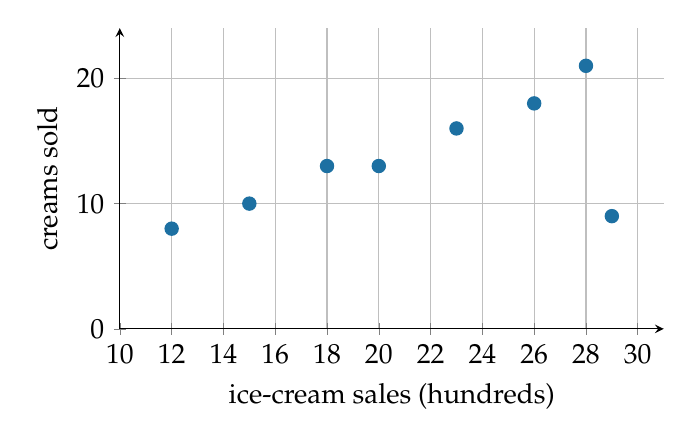
\begin{tikzpicture}
\begin{axis}[width=.7\textwidth,height=5.4cm,axis lines=left,xmin=10,xmax=31,ymin=0,ymax=24,grid=major,xtick={10,12,...,30},xlabel={ice-cream sales (hundreds)},ylabel={creams sold}]
\addplot[only marks,mark=*,Blue,mark size=2.4pt] coordinates {(12,8)(15,10)(18,13)(20,13)(23,16)(26,18)(28,21)(29,9)};
\end{axis}
\end{tikzpicture}
\end{center}
\begin{enumerate}
\item Describe the scatter plot: direction, shape and spread.
\item One point stands clearly apart from the others. Give its coordinates and suggest a plausible explanation.
\item The pharmacist claims: ``Ice creams cause sunburn.'' What do you think of this claim?
\item Suggest a factor that could explain why the two series change together.
\end{enumerate}
}{%
\begin{enumerate}
\item Apart from one point, the scatter plot is increasing: the weeks when the shop sells more ice cream are also the weeks when the pharmacy sells more creams. The points are fairly close to a straight line, with little spread.
\item The point $(29;9)$ is an outlier: very high ice-cream sales but few creams sold. Possible explanation: a cloudy week with a festival that attracted many visitors without strong sun exposure.
\item The scatter plot only shows that the two variables move in the same direction (correlation). It does not prove that one variable causes the other: the claim is not justified by these data.
\item Sunshine (or heat, or tourist numbers) increases both ice-cream sales and sunburn: it is a factor common to both series.
\end{enumerate}
}{4}

\DefExo{33}{Assessing and using a fitted line}{%
The manager of a gas-heated shop records, on some winter days, the average outdoor temperature $x_i$ (in °C) and the shop's gas consumption $y_i$ (in kWh).
\[
\begin{array}{c|rrrrrr}
x_i\text{ (°C)}&-4&-2&0&3&6&9\\\hline
y_i\text{ (kWh)}&62&55&50&41&32&24
\end{array}
\]
\begin{enumerate}
\item Plot the scatter plot on a coordinate grid, then calculate the coordinates of the mean point $G$.
\item An intern suggests the line $d_1$ with equation $y=-2x+50$. Draw it. Does this fit seem satisfactory? Justify using the point $G$.
\item From now on, the line $d_2$ with equation $y=-3x+50$ is used. Check that $G$ lies on $d_2$ and interpret the numbers $-3$ and $50$ in context.
\item Using $d_2$, estimate:
  \begin{itemize}
  \item the consumption on a day when it is $1$~°C;
  \item the consumption on a day when it is $12$~°C;
  \item the temperature on a day when the consumption is $35$~kWh.
  \end{itemize}
  For the first two estimates, state whether it is an interpolation or an extrapolation.
\end{enumerate}
}{%
\begin{enumerate}
\item Plot the six points. $\bar x=\dfrac{-4-2+0+3+6+9}{6}=\dfrac{12}{6}=2$ and $\bar y=\dfrac{62+55+50+41+32+24}{6}=\dfrac{264}{6}=44$, so $G(2;44)$. The scatter plot is decreasing and almost aligned.
\item For $x=2$, $d_1$ gives $y=-2\times2+50=46\neq44$: $d_1$ does not pass through $G$. Moreover, it is not steep enough: it runs below the first points ($58$ instead of $62$ at $-4$~°C) and well above the last ones ($32$ instead of $24$ at $9$~°C). The fit is not satisfactory.
\item $-3\times2+50=44$: $G\in d_2$. The coefficient $-3$ means that one more degree corresponds, on average, to about $3$~kWh less consumed; $50$ is the estimated consumption on a day at $0$~°C.
\item For $x=1$: $y=-3+50=47$, i.e.\ about $47$~kWh (interpolation, since $1\in[-4;9]$).\\
For $x=12$: $y=-36+50=14$, i.e.\ about $14$~kWh (extrapolation, since $12>9$: to be interpreted with caution).\\
$-3x+50=35$ is equivalent to $x=5$: a consumption of $35$~kWh corresponds to about $5$~°C.
\end{enumerate}
}{6}

\DefExo{34}{Linear regression and time-series forecast}{%
A regional operator records the number of subscribers to its fibre-optic offer on 31 December each year.
\[
\begin{array}{c|cccccc}
\text{Year}&2018&2019&2020&2021&2022&2023\\\hline
\text{Year rank }x_i&0&1&2&3&4&5\\
\text{Subscribers }y_i\text{ (thousands)}&8.2&11.5&13.9&17.4&20.1&23.8
\end{array}
\]
\begin{enumerate}
\item Plot the scatter plot of the points $M_i(x_i;y_i)$. Is a linear fit reasonable?
\item Using a calculator, find an equation of the least-squares regression line of $y$ on $x$. Round the coefficients to $10^{-2}$.
\item Assuming the trend continues, estimate the number of subscribers at the end of 2026.
\item According to this model, in which year would the number of subscribers exceed $40\,000$?
\end{enumerate}
}{%
\begin{enumerate}
\item The six points are almost aligned along an increasing straight line: a linear fit is relevant.
\item The calculator gives $a\approx3.0657$ and $b\approx8.1524$, hence the line $y=3.07x+8.15$.
\item The end of 2026 corresponds to rank $x=8$: $y=3.07\times8+8.15=32.71$. About $32\,710$ subscribers can be forecast. This is an extrapolation: the result assumes that the trend observed from 2018 to 2023 continues.
\item Solve $3.07x+8.15>40$, i.e.\ $x>\dfrac{40-8.15}{3.07}\approx10.37$. The first suitable whole rank is $x=11$ (check: $3.07\times10+8.15=38.85<40$ and $3.07\times11+8.15=41.92>40$). The threshold would be exceeded in $2018+11=2029$.
\end{enumerate}
}{6}

\DefExo{35}{Line through two points and careful extrapolation}{%
A logistics hub recorded the number of parcels shipped each year (in thousands).
\[
\begin{array}{c|ccccc}
\text{Year}&2019&2020&2021&2022&2023\\\hline
\text{Year rank }x_i&0&1&2&3&4\\
\text{Parcels shipped }y_i\text{ (thousands)}&212.4&268.0&341.7&398.2&463.6
\end{array}
\]
\begin{enumerate}
\item Plot the scatter plot of the points $M_1,\ldots,M_5$ on an orthogonal grid.
\item The scatter plot is fitted by the line $(M_1M_5)$ through the first and last points. Find an equation of this line (coefficients rounded to one decimal place if necessary).
\item Using this model, estimate the number of parcels shipped in 2027.
\item According to this model, in which year would the number of parcels shipped exceed one million?
\item Give two reasons why these forecasts may turn out to be unreliable.
\end{enumerate}
}{%
\begin{enumerate}
\item The five points are almost aligned along an increasing straight line.
\item $M_1(0;212.4)$ and $M_5(4;463.6)$. The gradient is $\dfrac{463.6-212.4}{4-0}=\dfrac{251.2}{4}=62.8$ and the intercept is $212.4$ (abscissa $0$). Equation: $y=62.8x+212.4$.
\item 2027 corresponds to rank $x=8$: $y=62.8\times8+212.4=714.8$, i.e.\ about $714\,800$ parcels.
\item One million parcels corresponds to $y=1\,000$. Solve $62.8x+212.4>1\,000$, i.e.\ $x>\dfrac{787.6}{62.8}\approx12.54$. The first whole rank is $x=13$ (check: $62.8\times12+212.4=966<1\,000$ and $62.8\times13+212.4=1\,028.8$). The threshold would be crossed in $2019+13=2032$.
\item These are extrapolations far from the observed period (2019--2023): the trend may change (competition, economic crisis, the hub reaching full capacity); moreover the line is built from only two points.
\end{enumerate}
}{6}

\DefExo{36}{Linearising with a logarithmic change of variable}{%
A marketing agency studies, for several clients, the monthly online advertising budget $x_i$ (in hundreds of euros) and the monthly number of visits $y_i$ to the client's website (in thousands).
\[
\begin{array}{c|rrrrrrrrrr}
x_i&1&2&4&5&8&10&15&20&30&40\\\hline
y_i&13&19&28&29&35&36&42&44&49&52
\end{array}
\]
Visits increase more and more slowly as the budget increases: a linear fit of $y$ on $x$ is not relevant. Let $u_i=\log(x_i)$.
\begin{enumerate}
\item Calculate the values $u_i$, rounded to two decimal places.
\item Plot the scatter plot of the points $(u_i;y_i)$. Using a calculator, find an equation of the least-squares regression line of $y$ on $u$ (coefficients rounded to one decimal place).
\item Deduce an expression of $y$ in terms of $x$.
\item Estimate the number of visits for a budget of $1\,200$~€, then of $6\,000$~€. Comment on the reliability of each estimate.
\end{enumerate}
}{%
\begin{enumerate}
\item $u_i$: $0$; $0.30$; $0.60$; $0.70$; $0.90$; $1$; $1.18$; $1.30$; $1.48$; $1.60$.
\item The scatter plot of $(u_i;y_i)$ is almost aligned. The calculator gives (with the rounded $u_i$) $a\approx24.59$ and $b\approx12.42$, hence $y=24.6u+12.4$.
\item Since $u=\log(x)$, we get $y=24.6\log(x)+12.4$.
\item $1\,200$~€ corresponds to $x=12$: $y=24.6\log(12)+12.4\approx38.9$, i.e.\ about $38\,900$ visits (interpolation, $12\in[1;40]$).\\
$6\,000$~€ corresponds to $x=60$: $y=24.6\log(60)+12.4\approx56.1$, i.e.\ about $56\,100$ visits. This is an extrapolation ($60>40$): the estimate should be interpreted with caution.
\end{enumerate}
}{6}

\DefExo{37}{Calibration: fit, residual and validity range}{%
A start-up is calibrating a low-cost carbon dioxide (CO$_2$) sensor intended for offices. Placed in chambers with a known concentration $C$ (in ppm, parts per million), the sensor delivers a voltage $U$ (in volts).
\[
\begin{array}{c|cccccc}
\text{Voltage }U\text{ (V)}&0.42&0.81&1.23&1.60&2.05&2.41\\\hline
\text{Concentration }C\text{ (ppm)}&400&800&1\,200&1\,600&2\,000&2\,400
\end{array}
\]
\begin{enumerate}
\item Plot the scatter plot of the points $(U;C)$, with $U$ on the horizontal axis.
\item Does a linear fit seem relevant? Using a calculator, find an equation of the regression line of $C$ on $U$, in the form $C=aU+b$ (coefficients rounded to the nearest unit).
\item Calculate the residual for $U=1.23$, that is, the difference between the actual concentration and the one given by the model. Comment.
\item In an office, the sensor reads $1.4$~V. Estimate the CO$_2$ concentration. A threshold of $1\,000$~ppm is often used as a guide for airing a room: should the room be aired?
\item Can this model be used with the same confidence for a voltage of $3.5$~V? Justify.
\end{enumerate}
}{%
\begin{enumerate}
\item The six points are almost aligned along an increasing straight line.
\item Yes. The calculator gives $a\approx996.59$ and $b\approx-15.16$, hence $C=997U-15$.
\item The model gives $997\times1.23-15=1\,211.31$. The residual is $1\,200-1\,211.31\approx-11$~ppm, i.e.\ less than $1\,\%$ of the value: the fit is good.
\item $C=997\times1.4-15=1\,380.8$, i.e.\ about $1\,381$~ppm (interpolation, since $1.4\in[0.42;2.41]$). This value exceeds $1\,000$~ppm: the room should be aired.
\item The model gives $997\times3.5-15=3\,474.5$~ppm, but $3.5$~V lies outside the calibration interval $[0.42;2.41]$: this is an extrapolation. Nothing guarantees that the sensor stays linear at high concentrations; the calibration should be extended.
\end{enumerate}
}{6}

\DefExo{38}{Mean point and regression line: justified choices}{%
For each question, exactly one option is correct. Choose it and justify.

Three stores of the same chain have a sales area $x$ (in hundreds of m$^2$) and a monthly turnover $y$ (in tens of thousands of euros) represented by the points $M_1(2;5)$, $M_2(4;11)$ and $M_3(6;11)$.
\begin{enumerate}
\item The mean point $G$ of this scatter plot is:
  \begin{enumerate}[label=\alph*.]
  \item the point $M_2$;
  \item the point with coordinates $(4;9)$;
  \item the point with coordinates $(12;27)$.
  \end{enumerate}
\item An equation of the line $(M_1M_3)$ is:
  \begin{enumerate}[label=\alph*.]
  \item $y=1.5x+2$;
  \item $y=2x+1$;
  \item $y=1.5x+3$.
  \end{enumerate}
\item The least-squares regression line obtained with a calculator:
  \begin{enumerate}[label=\alph*.]
  \item passes through the point $M_2$;
  \item passes through $G$ and has the same gradient as $(M_1M_3)$;
  \item passes through the origin.
  \end{enumerate}
\item Using this regression line, the estimated turnover of a $500$~m$^2$ store is:
  \begin{enumerate}[label=\alph*.]
  \item $95\,000$~€;
  \item $105\,000$~€;
  \item $110\,000$~€.
  \end{enumerate}
\end{enumerate}
}{%
\begin{enumerate}
\item Answer b: $\bar x=\dfrac{2+4+6}{3}=4$ and $\bar y=\dfrac{5+11+11}{3}=9$. Option c forgets to divide the sums by $3$.
\item Answer a: the gradient is $\dfrac{11-5}{6-2}=1.5$ and $5=1.5\times2+b$ gives $b=2$. The line $y=2x+1$ passes through $M_1$ but not through $M_3$ ($2\times6+1=13\neq11$).
\item Answer b: the calculator gives $y=1.5x+3$. It passes through $G$ ($1.5\times4+3=9$), has gradient $1.5$ like $(M_1M_3)$, and passes neither through $M_2$ ($1.5\times4+3=9\neq11$) nor through the origin ($b=3\neq0$).
\item Answer b: $500$~m$^2$ corresponds to $x=5$, and $y=1.5\times5+3=10.5$ tens of thousands of euros, i.e.\ $105\,000$~€ (interpolation).
\end{enumerate}
}{5}

% -----------------------------------------------------------------------------
% Chapter 6 -- Conditional probability
% -----------------------------------------------------------------------------
\DefExo{39}{Three-branch tree, total and reverse probability}{%
An online retailer hands its parcels to three carriers: $45\,\%$ to carrier $T_1$, $35\,\%$ to carrier $T_2$ and the rest to carrier $T_3$. Customer service finds that $2\,\%$ of the parcels delivered by $T_1$ arrive damaged, compared with $5\,\%$ for $T_2$ and $8\,\%$ for $T_3$.

A parcel is chosen at random. Let $T_i$ be the event ``The parcel is delivered by carrier $T_i$'' and $E$ the event ``The parcel arrives damaged''.
\begin{center}
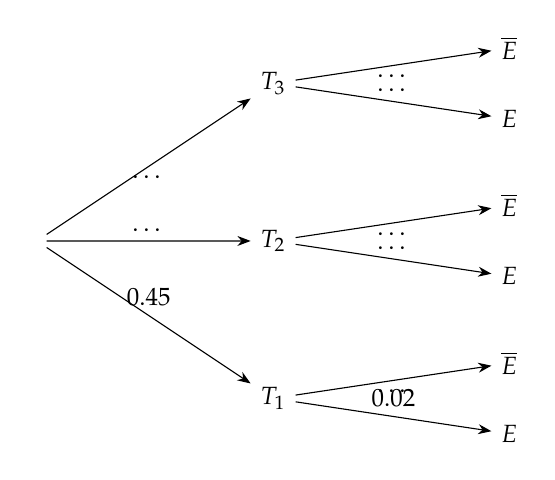
\begin{tikzpicture}[grow=right,level distance=30mm,level 1/.style={sibling distance=20mm},level 2/.style={sibling distance=9mm},every node/.style={font=\small},edge from parent/.style={draw,-{Stealth}}]
\node {}
 child {node {$T_1$}
   child {node {$E$} edge from parent node[above] {$0.02$}}
   child {node {$\overline E$} edge from parent node[below] {$\dots$}}
   edge from parent node[above] {$0.45$}}
 child {node {$T_2$}
   child {node {$E$} edge from parent node[above] {$\dots$}}
   child {node {$\overline E$} edge from parent node[below] {$\dots$}}
   edge from parent node[above] {$\dots$}}
 child {node {$T_3$}
   child {node {$E$} edge from parent node[above] {$\dots$}}
   child {node {$\overline E$} edge from parent node[below] {$\dots$}}
   edge from parent node[below] {$\dots$}};
\end{tikzpicture}
\end{center}
\begin{enumerate}
\item Copy and complete the weighted tree above.
\item Calculate the probability that the parcel is delivered by $T_3$ and arrives damaged.
\item Show that the probability that a parcel arrives damaged is equal to $0.0425$.
\item A customer reports a damaged parcel. What is the probability that it was delivered by $T_3$? Round to $10^{-3}$.
\end{enumerate}
}{%
\begin{enumerate}
\item $P(T_3)=1-0.45-0.35=0.20$. Second-level branches: $P_{T_1}(\overline E)=0.98$; $P_{T_2}(E)=0.05$ and $P_{T_2}(\overline E)=0.95$; $P_{T_3}(E)=0.08$ and $P_{T_3}(\overline E)=0.92$.
\item $P(T_3\cap E)=P(T_3)\times P_{T_3}(E)=0.20\times0.08=0.016$.
\item $T_1$, $T_2$, $T_3$ form a partition of the sample space. By the law of total probability:
$P(E)=0.45\times0.02+0.35\times0.05+0.20\times0.08=0.009+0.0175+0.016=0.0425$.
\item $P_E(T_3)=\dfrac{P(T_3\cap E)}{P(E)}=\dfrac{0.016}{0.0425}\approx0.376$. Although $T_3$ carries only $20\,\%$ of the parcels, it accounts for about $37.6\,\%$ of the damaged parcels.
\end{enumerate}
}{5}

\DefExo{40}{Completing a tree and computing intersections}{%
In this exercise, results are given as fractions in lowest terms. Consider the weighted tree below, where $E$ is an event and $R$, $S$ and $T$ form a partition of the sample space.
\begin{center}
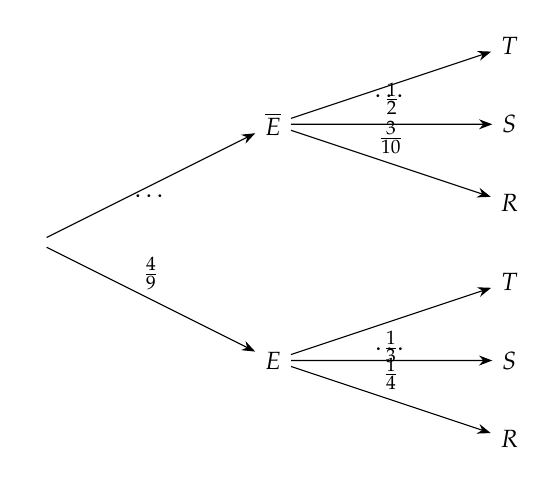
\begin{tikzpicture}[grow=right,level distance=30mm,level 1/.style={sibling distance=30mm},level 2/.style={sibling distance=10mm},every node/.style={font=\small},edge from parent/.style={draw,-{Stealth}}]
\node {}
 child {node {$E$}
   child {node {$R$} edge from parent node[above] {$\tfrac14$}}
   child {node {$S$} edge from parent node[above] {$\dots$}}
   child {node {$T$} edge from parent node[below] {$\tfrac13$}}
   edge from parent node[above] {$\tfrac49$}}
 child {node {$\overline E$}
   child {node {$R$} edge from parent node[above] {$\tfrac3{10}$}}
   child {node {$S$} edge from parent node[above] {$\tfrac12$}}
   child {node {$T$} edge from parent node[below] {$\dots$}}
   edge from parent node[below] {$\dots$}};
\end{tikzpicture}
\end{center}
\begin{enumerate}
\item Complete the tree, justifying each calculation.
\item Calculate $P(E\cap R)$ and $P(\overline E\cap S)$.
\item Calculate $P(T)$.
\end{enumerate}
}{%
\begin{enumerate}
\item The branches leaving the same node add up to $1$: $P(\overline E)=1-\dfrac49=\dfrac59$; $P_E(S)=1-\dfrac14-\dfrac13=\dfrac5{12}$; $P_{\overline E}(T)=1-\dfrac3{10}-\dfrac12=\dfrac15$.
\item $P(E\cap R)=\dfrac49\times\dfrac14=\dfrac19$ and $P(\overline E\cap S)=\dfrac59\times\dfrac12=\dfrac5{18}$.
\item $E$ and $\overline E$ form a partition, so
$P(T)=P(E\cap T)+P(\overline E\cap T)=\dfrac49\times\dfrac13+\dfrac59\times\dfrac15=\dfrac4{27}+\dfrac19=\dfrac4{27}+\dfrac3{27}=\dfrac7{27}$.
\end{enumerate}
}{5}

\DefExo{41}{Translating an event, product along a path}{%
In a gym, $65\,\%$ of members have an annual membership, the others a monthly membership. Each member chooses a main activity. Among annual members, $50\,\%$ choose weight training, $30\,\%$ group classes and the rest swimming. Among monthly members, $40\,\%$ choose weight training, $45\,\%$ group classes and the rest swimming.

A member is chosen at random. Let $A$: ``The member has an annual membership'', $M$: ``Their main activity is weight training'', $C$: ``Their main activity is a group class'' and $N$: ``Their main activity is swimming''.
\begin{enumerate}
\item Draw a weighted tree describing the situation.
\item Describe the event $\overline A\cap C$ in a sentence, then calculate its probability.
\item Calculate the probability that the chosen member's main activity is swimming.
\item The chosen member mainly swims. Calculate the probability that they have an annual membership. Round to $10^{-3}$.
\end{enumerate}
}{%
\begin{enumerate}
\item First level: $P(A)=0.65$ and $P(\overline A)=0.35$. Under $A$: $P_A(M)=0.50$, $P_A(C)=0.30$, $P_A(N)=1-0.50-0.30=0.20$. Under $\overline A$: $P_{\overline A}(M)=0.40$, $P_{\overline A}(C)=0.45$, $P_{\overline A}(N)=1-0.40-0.45=0.15$.
\item $\overline A\cap C$: ``The member has a monthly membership and their main activity is a group class''. $P(\overline A\cap C)=0.35\times0.45=0.1575$.
\item By the law of total probability ($A$, $\overline A$ form a partition): $P(N)=0.65\times0.20+0.35\times0.15=0.13+0.0525=0.1825$.
\item $P_N(A)=\dfrac{P(A\cap N)}{P(N)}=\dfrac{0.13}{0.1825}\approx0.712$.
\end{enumerate}
}{6}

\DefExo{42}{Using and testing independence}{%
In a call centre, a call is chosen at random. Let $A$ be the event ``The customer waits more than $5$ minutes before being answered'' and $B$ the event ``The call is cut off because of a network incident''. We know that $P(A)=0.12$ and $P(B)=0.05$. In questions 1 to 3, assume that $A$ and $B$ are independent.
\begin{enumerate}
\item Calculate the probability that the customer waits more than $5$ minutes and that the call is cut off.
\item Calculate the probability that neither of these two incidents occurs.
\item Deduce the probability that at least one of the two incidents occurs.
\item An audit actually shows that, among calls with a wait of more than $5$ minutes, $9\,\%$ are cut off. Is the independence assumption confirmed? Justify.
\end{enumerate}
}{%
\begin{enumerate}
\item By independence, $P(A\cap B)=P(A)\times P(B)=0.12\times0.05=0.006$.
\item If $A$ and $B$ are independent, so are $\overline A$ and $\overline B$: $P(\overline A\cap\overline B)=0.88\times0.95=0.836$.
\item The event ``at least one incident'' is the complement of ``no incident'': its probability is $1-0.836=0.164$.
\item The audit gives $P_A(B)=0.09$, whereas $P(B)=0.05$. Since $P_A(B)\neq P(B)$, $A$ and $B$ are not independent: a long wait goes together with a cut-off more often.
\end{enumerate}
}{5}

\DefExo{43}{From a two-way table to weighted trees}{%
A group employs $1\,600$ staff across three sites: the head office, the factory and the warehouse. The staff who work from home at least one day a week have been counted.
\[
\begin{array}{l|ccc}
&\text{Remote work}&\text{No remote work}&\text{Total}\\\hline
\text{Head office}&300&\cdots&400\\
\text{Factory}&\cdots&\cdots&\cdots\\
\text{Warehouse}&\cdots&340&400\\\hline
\text{Total}&420&\cdots&1\,600
\end{array}
\]
\begin{enumerate}
\item Complete the table.
\item An employee is chosen at random. Let $S_1$: ``They work at the head office'', $S_2$: ``They work at the factory'', $S_3$: ``They work at the warehouse'' and $T$: ``They work from home''. Draw the weighted tree whose first level is $S_1$, $S_2$, $S_3$ and second level is $T$, $\overline T$.
\item Draw the weighted tree whose first level is $T$, $\overline T$ and second level is $S_1$, $S_2$, $S_3$. Give the probabilities as fractions in lowest terms, then rounded to $10^{-3}$.
\end{enumerate}
}{%
\begin{enumerate}
\item Head office: $400-300=100$ without remote work. Warehouse: $400-340=60$ with remote work. Factory: $1\,600-400-400=800$ staff, of whom $420-300-60=60$ work from home and $800-60=740$ do not. Total without remote work: $100+740+340=1\,180$ ($=1\,600-420$).
\item $P(S_1)=\dfrac{400}{1\,600}=0.25$, $P(S_2)=\dfrac{800}{1\,600}=0.5$, $P(S_3)=0.25$.\\
$P_{S_1}(T)=\dfrac{300}{400}=0.75$ and $P_{S_1}(\overline T)=0.25$; $P_{S_2}(T)=\dfrac{60}{800}=0.075$ and $P_{S_2}(\overline T)=0.925$; $P_{S_3}(T)=\dfrac{60}{400}=0.15$ and $P_{S_3}(\overline T)=0.85$.
\item $P(T)=\dfrac{420}{1\,600}=\dfrac{21}{80}=0.2625$ and $P(\overline T)=\dfrac{59}{80}=0.7375$.\\
$P_T(S_1)=\dfrac{300}{420}=\dfrac57\approx0.714$, $P_T(S_2)=\dfrac{60}{420}=\dfrac17\approx0.143$, $P_T(S_3)=\dfrac17\approx0.143$.\\
$P_{\overline T}(S_1)=\dfrac{100}{1\,180}=\dfrac5{59}\approx0.085$, $P_{\overline T}(S_2)=\dfrac{740}{1\,180}=\dfrac{37}{59}\approx0.627$, $P_{\overline T}(S_3)=\dfrac{340}{1\,180}=\dfrac{17}{59}\approx0.288$.\\
Check: the fractions leaving each node add up to $1$.
\end{enumerate}
}{7}

\DefExo{44}{Reversing a conditional probability}{%
A DIY chain surveys its customers. $45\,\%$ of them have downloaded the chain's loyalty app; among these, $60\,\%$ made at least one purchase on special offer during the last month. Overall, $36\,\%$ of the customers surveyed made at least one purchase on special offer during the last month.

A surveyed customer is chosen at random. Let $A$: ``The customer has downloaded the app'' and $R$: ``The customer made at least one purchase on special offer last month''.
\begin{enumerate}
\item Give $P(A)$, $P(R)$ and $P_A(R)$.
\item Calculate $P(A\cap R)$, then $P_R(A)$. Interpret the latter result.
\item Calculate the probability that a customer who has not downloaded the app made a purchase on special offer. Round to $10^{-3}$ and compare with $P_A(R)$.
\end{enumerate}
}{%
\begin{enumerate}
\item $P(A)=0.45$, $P(R)=0.36$ and $P_A(R)=0.60$.
\item $P(A\cap R)=P(A)\times P_A(R)=0.45\times0.60=0.27$. Then $P_R(A)=\dfrac{P(A\cap R)}{P(R)}=\dfrac{0.27}{0.36}=0.75$: three quarters of the customers who bought on special offer have downloaded the app.
\item $P(\overline A\cap R)=P(R)-P(A\cap R)=0.36-0.27=0.09$ and $P(\overline A)=0.55$, so $P_{\overline A}(R)=\dfrac{0.09}{0.55}\approx0.164$. This is much less than $P_A(R)=0.60$: customers with the app buy on special offer far more often.
\end{enumerate}
}{4}

\DefExo{45}{Two-stage experiment, fractional results}{%
In this exercise, results are given as fractions in lowest terms. During a promotional event, a customer draws one ticket at random from ten tickets numbered $1$ to $10$.
\begin{itemize}
\item If the number is $1$ or $2$, they scratch a card taken at random from box X, which contains $3$ winning cards out of $8$.
\item If the number is a multiple of $3$, they scratch a card from box Y, which contains $2$ winning cards out of $9$.
\item Otherwise, they scratch a card from box Z, which contains $1$ winning card out of $6$.
\end{itemize}
Let $X$, $Y$, $Z$ be the events ``The card comes from box X'' (Y, Z respectively) and $G$ the event ``The card is a winning card''.
\begin{enumerate}
\item Justify that $P(X)=\dfrac15$, $P(Y)=\dfrac3{10}$ and $P(Z)=\dfrac12$, then represent the situation with a weighted tree.
\item Prove that the probability that the card is a winning card is equal to $\dfrac9{40}$.
\item The customer has won. What is the probability that their card came from box X?
\end{enumerate}
}{%
\begin{enumerate}
\item The ten numbers are equally likely. $X$ corresponds to $\{1;2\}$: $P(X)=\dfrac2{10}=\dfrac15$. $Y$ corresponds to $\{3;6;9\}$: $P(Y)=\dfrac3{10}$. $Z$ corresponds to the five other numbers $\{4;5;7;8;10\}$: $P(Z)=\dfrac5{10}=\dfrac12$.\\
Tree: under $X$, $P_X(G)=\dfrac38$ and $P_X(\overline G)=\dfrac58$; under $Y$, $P_Y(G)=\dfrac29$ and $P_Y(\overline G)=\dfrac79$; under $Z$, $P_Z(G)=\dfrac16$ and $P_Z(\overline G)=\dfrac56$.
\item $X$, $Y$, $Z$ form a partition:
$P(G)=\dfrac15\times\dfrac38+\dfrac3{10}\times\dfrac29+\dfrac12\times\dfrac16=\dfrac3{40}+\dfrac1{15}+\dfrac1{12}=\dfrac{9}{120}+\dfrac{8}{120}+\dfrac{10}{120}=\dfrac{27}{120}=\dfrac9{40}$.
\item $P_G(X)=\dfrac{P(X\cap G)}{P(G)}=\dfrac{3/40}{9/40}=\dfrac13$.
\end{enumerate}
}{6}

\DefExo{46}{Review: path, complement and independent repetition}{%
A business incubator selects the projects it supports in three stages. $30\,\%$ of the applications submitted pass the pre-selection. Pre-selected projects are presented to a panel, which keeps $50\,\%$ of them. Finally, an investors' committee funds $20\,\%$ of the projects kept by the panel. A project eliminated at one stage does not go on to the following stages.

An application is chosen at random. Let $P$: ``The application passes the pre-selection'', $J$: ``The project is kept by the panel'' and $F$: ``The project is funded''.
\begin{enumerate}
\item Draw a weighted tree describing the situation. Prove that the probability that a project is not funded is equal to $0.97$.
\item Eight entrepreneurs submit an application; assume that the applications are examined independently of one another. Calculate the probability that at least one of the eight projects is funded. Round to $10^{-3}$.
\item What is the minimum number of applications the incubator must receive for the probability of funding at least one project to exceed $0.99$?
\end{enumerate}
}{%
\begin{enumerate}
\item Tree: $P$ ($0.30$) or $\overline P$ ($0.70$, end); after $P$: $J$ ($0.50$) or $\overline J$ ($0.50$, end); after $J$: $F$ ($0.20$) or $\overline F$ ($0.80$). A project is funded only if it passes all three stages, so, multiplying along this path:
$P(F)=0.30\times0.50\times0.20=0.03$ and $P(\overline F)=1-0.03=0.97$.
\item By independence, the probability that none of the eight projects is funded is $0.97^8$. The required probability is $1-0.97^8\approx0.216$.
\item We look for the smallest whole number $n$ such that $1-0.97^n>0.99$, i.e.\ $0.97^n<0.01$. Since $\log$ is increasing, this is equivalent to $n\log(0.97)<\log(0.01)$, i.e.\ $n>\dfrac{\log(0.01)}{\log(0.97)}\approx151.2$ (dividing by $\log(0.97)<0$ reverses the inequality). At least $152$ applications are needed (check: $1-0.97^{151}\approx0.98994$ and $1-0.97^{152}\approx0.99024$).
\end{enumerate}
}{6}

% Original exercises -- sessions 47 to 55 (chapter 7: discrete random
% variables and the binomial distribution; chapter 8: revision and consolidation).
% Format: \DefExo{session}{target}{statement}{detailed solution}{answer lines}

% -----------------------------------------------------------------------------
% Chapter 7 -- Discrete random variables and the binomial distribution
% -----------------------------------------------------------------------------
\DefExo{47}{Distribution of a gain and expected value}{%
To launch a new perfume, a cosmetics chain sells its customers a scratch card for €$3$. The cards are printed in booklets of $25$: in each booklet, $16$ cards are losing cards, $6$ cards give a €$6$ shopping voucher and $3$ cards give a €$13$ shopping voucher. A customer buys a card chosen at random from a new booklet.

Let $G$ be the random variable equal to the customer's net gain, in euros, that is, the value of the voucher obtained minus the price of the card (a negative gain is a loss).
\begin{enumerate}
\item What values does $G$ take?
\item Copy and complete the following table, which gives the probability distribution of $G$.
\begin{center}
\renewcommand{\arraystretch}{1.4}
\begin{tabular}{|l|*{3}{p{1.7cm}|}}
\hline
Value $g_i$ of $G$ & & & \\
\hline
$P(G=g_i)$ & & & \\
\hline
\end{tabular}
\end{center}
\item Calculate the expected value $E(G)$. What can be said from the customer's point of view? And from the chain's point of view?
\item The chain wants to earn €$0.40$ on average per card sold, without changing the composition of the booklets. At what price should it sell the card?
\end{enumerate}
}{%
\begin{enumerate}
\item A losing card gives $G=0-3=-3$; a €$6$ voucher gives $G=6-3=3$; a €$13$ voucher gives $G=13-3=10$. So $G$ takes the values $-3$, $3$ and $10$.
\item The card is chosen at random among $25$ cards: all outcomes are equally likely.
\[
\begin{array}{|l|c|c|c|}\hline
g_i&-3&3&10\\\hline
P(G=g_i)&\dfrac{16}{25}=0.64&\dfrac{6}{25}=0.24&\dfrac{3}{25}=0.12\\\hline
\end{array}
\]
Check: $0.64+0.24+0.12=1$.
\item $E(G)=-3\times0.64+3\times0.24+10\times0.12=-1.92+0.72+1.20=0$.
The expected value is zero: over a large number of cards, the customer neither wins nor loses on average; the game is fair. The chain earns nothing on average from the cards themselves: the operation only serves to attract customers.
\item Let $B$ be the value of the voucher. $E(B)=0\times0.64+6\times0.24+13\times0.12=1.44+1.56=3$ euros. If the card costs $c$ euros, the customer's net gain is $B-c$ and its expected value is $3-c$ (each value of $G$ is decreased by $c$). We want $3-c=-0.40$, so $c=3.40$ euros.
Check: the values become $-3.40$, $2.60$, $9.60$ and $-3.40\times0.64+2.60\times0.24+9.60\times0.12=-2.176+0.624+1.152=-0.40$.
\end{enumerate}
}{5}

\DefExo{48}{Recognising a binomial distribution, n = 2}{%
On a large online sales platform, $12\,\%$ of shipped parcels are returned by the customer. The quality department chooses two shipped parcels at random. The number of shipped parcels is large enough for this choice to be treated as two random draws with replacement.

Let $R$ be the event ``the parcel is returned'' and $X$ the random variable equal to the number of returned parcels among the two chosen parcels.
\begin{center}
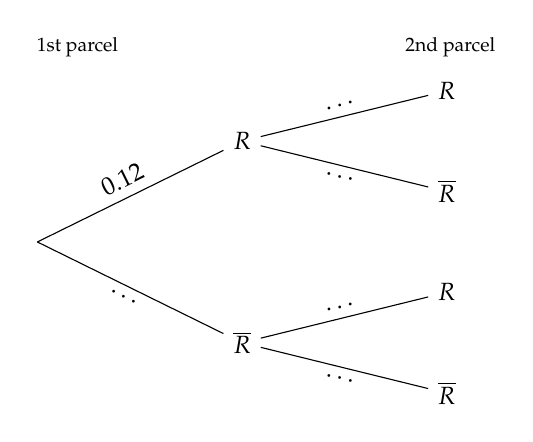
\begin{tikzpicture}[font=\small,x=26mm,y=8mm]
\coordinate (O) at (0,0);
\node (R1) at (1,1.6) {$R$};
\node (N1) at (1,-1.6) {$\overline R$};
\node (RR) at (2,2.4) {$R$};
\node (RN) at (2,0.8) {$\overline R$};
\node (NR) at (2,-0.8) {$R$};
\node (NN) at (2,-2.4) {$\overline R$};
\draw (O)--node[above,sloped]{$0.12$}(R1);
\draw (O)--node[below,sloped]{$\dots$}(N1);
\draw (R1)--node[above,sloped]{$\dots$}(RR);
\draw (R1)--node[below,sloped]{$\dots$}(RN);
\draw (N1)--node[above,sloped]{$\dots$}(NR);
\draw (N1)--node[below,sloped]{$\dots$}(NN);
\node[anchor=west,font=\scriptsize] at (-0.05,3.1) {1st parcel};
\node[anchor=west,font=\scriptsize] at (1.75,3.1) {2nd parcel};
\end{tikzpicture}
\end{center}
\begin{enumerate}
\item Copy and complete the weighted tree above.
\item Justify that $X$ follows a binomial distribution and give its parameters.
\item Calculate $P(X=0)$, $P(X=1)$ and $P(X=2)$. For $P(X=1)$, state how many paths of the tree give the event $\{X=1\}$.
\item Deduce, in two different ways, the probability that at least one of the two parcels is returned.
\end{enumerate}
}{%
\begin{enumerate}
\item First level: $P(R)=0.12$ and $P(\overline R)=1-0.12=0.88$. Since the draws are treated as draws with replacement, the second level uses the same probabilities: $0.12$ towards $R$ and $0.88$ towards $\overline R$ on each of the two branches.
\item A Bernoulli trial whose success ``the parcel is returned'' has probability $0.12$ is repeated $2$ times, identically and independently (draws treated as draws with replacement). The variable $X$ counts the successes: $X$ follows the binomial distribution $\mathcal B(2;0.12)$.
\item $P(X=0)=0.88^2=0.7744$.
Two paths give $\{X=1\}$: $(R,\overline R)$ and $(\overline R,R)$, hence $P(X=1)=2\times0.12\times0.88=0.2112$.
$P(X=2)=0.12^2=0.0144$.
Check: $0.7744+0.2112+0.0144=1$.
\item ``At least one return'' is the event $\{X\geqslant1\}$.
By addition: $P(X\geqslant1)=P(X=1)+P(X=2)=0.2112+0.0144=0.2256$.
Using the complementary event: $P(X\geqslant1)=1-P(X=0)=1-0.7744=0.2256$.
So there is about a $22.6\,\%$ chance that at least one of the two parcels is returned.
\end{enumerate}
}{5}

\DefExo{49}{Pascal's triangle and B(n; 1/2)}{%
An online shop is testing two layouts of its home page (A/B test): for each new visitor, the site displays version A or version B at random, with the same probability $\dfrac12$, independently of the other visitors. The next $7$ visitors are observed and $X$ denotes the random variable equal to the number of visitors who are shown version B.
\begin{enumerate}
\item Justify that $X$ follows a binomial distribution and give its parameters.
\item Build Pascal's triangle up to row $n=7$.
\item Read $\binom73$ in the triangle and interpret this number in context. Calculate $P(X=3)$ as a fraction, then rounded to $10^{-3}$. Interpret the result.
\item Calculate the probability that at least $5$ of the $7$ visitors see version B (as a fraction, then rounded to $10^{-3}$).
\end{enumerate}
}{%
\begin{enumerate}
\item Each visitor is a Bernoulli trial whose success ``version B is displayed'' has probability $\dfrac12$. The $7$ trials are identical and independent, and $X$ counts the successes: $X\sim\mathcal B\left(7;\dfrac12\right)$.
\item
\begin{center}
\begin{tabular}{c|*{8}{c}}
$n$&\multicolumn{8}{l}{coefficients $\binom nk$ for $k=0,\dots,n$}\\\hline
$0$&1\\
$1$&1&1\\
$2$&1&2&1\\
$3$&1&3&3&1\\
$4$&1&4&6&4&1\\
$5$&1&5&10&10&5&1\\
$6$&1&6&15&20&15&6&1\\
$7$&1&7&21&35&35&21&7&1
\end{tabular}
\end{center}
Each inner coefficient is the sum of the coefficient directly above it and the coefficient to the left of that one (for example $\binom73=\binom62+\binom63=15+20=35$).
\item $\binom73=35$: there are $35$ different sequences of $7$ displays containing version B exactly $3$ times. Each sequence has probability $\left(\dfrac12\right)^3\left(\dfrac12\right)^4=\dfrac1{128}$, so
$P(X=3)=\dfrac{35}{128}\approx0.273$. In about $27\,\%$ of series of $7$ visitors, exactly $3$ see version B.
\item $P(X\geqslant5)=P(X=5)+P(X=6)+P(X=7)=\dfrac{21+7+1}{128}=\dfrac{29}{128}\approx0.227$.
\end{enumerate}
}{5}

\DefExo{50}{Binomial probabilities, triangle up to n = 8}{%
In a medical practice, it is estimated that a patient who booked an appointment online actually turns up for the consultation with probability $0.9$. One morning, a doctor has $8$ appointments booked online. Let $X$ be the random variable equal to the number of patients who turn up among these $8$. Assume that $X$ follows a binomial distribution.

Probabilities will be rounded to $10^{-3}$.
\begin{enumerate}
\item Give the parameters $n$ and $p$ of the distribution of $X$.
\item Calculate the probability of the following events:
$A$: ``all $8$ patients turn up''; $B$: ``at least one patient does not turn up''.
\item Build Pascal's triangle up to row $n=8$. Deduce $\binom86$, then the probability of the event $C$: ``exactly $6$ patients turn up''.
\item Express the event $\{X=7\}$ in a sentence, then calculate $P(X=7)$.
\end{enumerate}
}{%
\begin{enumerate}
\item $n=8$ and $p=0.9$: $X\sim\mathcal B(8;0.9)$.
\item $P(A)=P(X=8)=0.9^8\approx0.430$.
$B$ is the complementary event of $A$: $P(B)=1-0.9^8\approx0.570$.
\item Row $8$ of the triangle (obtained from row $7$: $1,7,21,35,35,21,7,1$): $1,8,28,56,70,56,28,8,1$. So $\binom86=28$.
$P(C)=P(X=6)=28\times0.9^6\times0.1^2\approx0.149$.
\item $\{X=7\}$: ``exactly $7$ of the $8$ patients turn up'', that is, exactly one patient is absent.
$P(X=7)=\binom87\times0.9^7\times0.1=8\times0.9^7\times0.1\approx0.383$.
\end{enumerate}
}{5}

\DefExo{51}{Review: binomial law, at least, expected value}{%
A vegetable seed producer claims that $95\,\%$ of its tomato seeds germinate. The seeds are sold in packets of $12$. Production is large enough for filling a packet to be treated as a random draw with replacement of $12$ seeds. Let $X$ be the random variable that associates with each packet the number of seeds that germinate.
\begin{enumerate}
\item What distribution does $X$ follow? Justify and give its parameters.
\item Give $\binom{12}{11}$ and $\binom{12}{12}$.
\item Calculate $P(X=11)$ and $P(X=12)$, rounded to $10^{-3}$. Interpret each of these results.
\item Deduce the probability, rounded to $10^{-3}$, that a packet contains at least $11$ seeds that germinate.
\item Calculate $E(X)$ and interpret this number for a gardener who regularly buys these packets.
\end{enumerate}
}{%
\begin{enumerate}
\item The Bernoulli trial ``a seed germinates'', with probability $0.95$, is repeated $12$ times, identically and independently (draw treated as a draw with replacement). $X$ counts the successes: $X\sim\mathcal B(12;0.95)$.
\item $\binom{12}{11}=12$ (choose the only seed that does not germinate) and $\binom{12}{12}=1$.
\item $P(X=11)=12\times0.95^{11}\times0.05\approx0.341$: about $34\,\%$ of packets contain exactly one seed that does not germinate.
$P(X=12)=0.95^{12}\approx0.540$: in about $54\,\%$ of packets, all the seeds germinate.
\item $P(X\geqslant11)=P(X=11)+P(X=12)=12\times0.95^{11}\times0.05+0.95^{12}\approx0.882$ (computed with the unrounded values; adding the rounded values would give $0.881$).
\item $E(X)=np=12\times0.95=11.4$. Over a large number of packets, an average of $11.4$ seeds germinate per packet; this is not a value that $X$ can take for a given packet.
\end{enumerate}
}{6}

% -----------------------------------------------------------------------------
% Sessions 52 to 55 -- Consolidation
% -----------------------------------------------------------------------------
\DefExo{52}{Rates of change, geometric mean, geometric sequence}{%
A cooperative installs home solar kits in a rural region. The table below gives the number of kits installed each year.
\[
\begin{array}{c|ccc}
\text{Year}&2021&2022&2023\\\hline
\text{Number of kits installed}&2\,480&3\,150&3\,938
\end{array}
\]
\textbf{Part A}
\begin{enumerate}
\item Calculate the rate of change in the number of kits installed between 2021 and 2022, then between 2022 and 2023 (as a percentage, rounded to $0.1\,\%$).
\item Calculate the geometric mean of $1.27$ and $1.25$ (rounded to $10^{-4}$).
\item Deduce the average annual rate of change between 2021 and 2023.
\end{enumerate}
\textbf{Part B}

Assume that from 2023 onwards, the number of kits installed increases by $26\,\%$ per year. Let $u_n$ be the number of kits installed during the year $2023+n$, values being rounded to the nearest unit.
\begin{enumerate}
\item Give $u_0$, then calculate $u_1$ and $u_2$.
\item What kind of sequence is $(u_n)$? Express $u_n$ in terms of $n$.
\item According to this model, how many kits would be installed in 2028?
\item Using a calculator, determine the year from which the annual number of kits installed would exceed $20\,000$.
\end{enumerate}
}{%
\textbf{Part A}
\begin{enumerate}
\item $\dfrac{3\,150-2\,480}{2\,480}\approx0.270$, an increase of about $27.0\,\%$; $\dfrac{3\,938-3\,150}{3\,150}\approx0.250$, an increase of about $25.0\,\%$. The multipliers are therefore about $1.27$ and $1.25$.
\item $\sqrt{1.27\times1.25}=\sqrt{1.5875}\approx1.2600$.
\item The average annual multiplier is about $1.26$: the average annual rate is about $26.0\,\%$ (direct check: $\sqrt{3\,938/2\,480}\approx1.2601$).
\end{enumerate}
\textbf{Part B}
\begin{enumerate}
\item $u_0=3\,938$; $u_1=3\,938\times1.26\approx4\,962$; $u_2=3\,938\times1.26^2\approx6\,252$.
\item An increase of $26\,\%$ means multiplying by $1.26$: $(u_n)$ is geometric with first term $u_0=3\,938$ and common ratio $q=1.26$, so $u_n=3\,938\times1.26^n$.
\item 2028 corresponds to $n=5$: $u_5=3\,938\times1.26^5\approx12\,506$ kits.
\item From the table of values: $u_7\approx19\,855<20\,000$ and $u_8\approx25\,017>20\,000$. Since the ratio is greater than $1$, the sequence is increasing: the threshold is exceeded from $n=8$ onwards, that is, in 2031.
\end{enumerate}
}{7}

\DefExo{53}{Average annual rate over three years}{%
The number of visitors to a nature park went through three successive annual changes: an increase of $5.4\,\%$, then a decrease of $2.6\,\%$, then an increase of $7.1\,\%$.
\begin{enumerate}
\item Calculate the overall multiplier over the three years and the corresponding overall rate of change (rounded to $0.01\,\%$).
\item Calculate the average annual rate of change over this period (rounded to $0.01\,\%$).
\item The initial number of visitors was $85\,000$. Calculate the final number of visitors, then check that an increase at this average rate applied three times leads to roughly the same result.
\end{enumerate}
}{%
\begin{enumerate}
\item The multipliers are $1.054$, $1-0.026=0.974$ and $1.071$. Overall multiplier: $1.054\times0.974\times1.071\approx1.099\,48$, an overall increase of about $9.95\,\%$.
\item The average annual multiplier $c_m$ satisfies $c_m^3=1.099\,48$, so $c_m=1.099\,48^{1/3}\approx1.0321$. The average annual rate is about $3.21\,\%$.
\item Final number of visitors: $85\,000\times1.054\times0.974\times1.071\approx93\,456$. With the average rate: $85\,000\times1.0321^3\approx93\,451$ visitors; the difference only comes from rounding $c_m$.
\end{enumerate}
}{4}

\DefExo{54}{Order of magnitude and common logarithm}{%
\emph{Definition.} The order of magnitude of a real number $x>0$ is the power of $10$ closest to $x$ (compare the distances from $x$ to the two powers of $10$ on either side of it).
\begin{enumerate}
\item Consider $x=27.6$ and $y=812$.
  \begin{enumerate}[label=\alph*.]
  \item Give the order of magnitude of $x$ and of $y$, justifying with a calculation of distances.
  \item Using a calculator, give $\log(x)$ and $\log(y)$ rounded to $10^{-3}$. Make a conjecture: how can the order of magnitude be obtained from the logarithm rounded to the nearest unit?
  \end{enumerate}
\item Consider $z=4.6$. Determine its order of magnitude and $\log(z)$. Does the conjecture of question 1 hold?
\item Write $x$ in scientific notation: $x=a\times10^n$ with $1\leqslant a<10$ and $n$ an integer. Depending on the value of $a$, what is the order of magnitude of $x$? (If the distances are equal, take the larger power.)
\item Express $\log(x)$ in terms of $n$ and $\log(a)$. Deduce a method for obtaining $n$, $a$ and then the order of magnitude of $x$ from $\log(x)$.
\item In cybersecurity, the strength of a key or a password is assessed by the number of possibilities. A calculator cannot display the following numbers directly. Determine the order of magnitude of:
  \begin{enumerate}[label=\alph*.]
  \item the number $2^{1\,024}$ of $1\,024$-bit keys;
  \item the number $94^{128}$ of $128$-character passwords chosen from $94$ characters.
  \end{enumerate}
\end{enumerate}
}{%
\begin{enumerate}
\item
  \begin{enumerate}[label=\alph*.]
  \item $10<27.6<100$: $27.6-10=17.6$ and $100-27.6=72.4$, so the order of magnitude of $x$ is $10$. $100<812<1\,000$: $812-100=712$ and $1\,000-812=188$, so that of $y$ is $10^3$.
  \item $\log(27.6)\approx1.441$ and $\log(812)\approx2.910$. Rounded to the nearest unit: $1$ and $3$. Conjecture: ``the order of magnitude of $x$ is $10^{k}$, where $k$ is $\log(x)$ rounded to the nearest unit''.
  \end{enumerate}
\item $1<4.6<10$: $4.6-1=3.6$ and $10-4.6=5.4$, so the order of magnitude of $z$ is $1=10^0$. But $\log(4.6)\approx0.663$, which rounds to $1$: the conjecture would give $10^1$. It is false ($z$ is a counterexample).
\item $x$ lies between $10^n$ and $10^{n+1}$, whose midpoint is $\dfrac{10^n+10^{n+1}}2=5.5\times10^n$. So the order of magnitude is $10^n$ if $a<5.5$, and $10^{n+1}$ if $a\geqslant5.5$.
\item $\log(x)=\log(a)+\log(10^n)=n+\log(a)$, with $0\leqslant\log(a)<1$. Method: $n$ is the integer part of $\log(x)$; $a=10^{\log(x)-n}$; compare $a$ with $5.5$ (which amounts to comparing $\log(x)-n$ with $\log(5.5)\approx0.740$, not with $0.5$).
\item
  \begin{enumerate}[label=\alph*.]
  \item $\log(2^{1\,024})=1\,024\log(2)\approx308.255$. So $n=308$, $a=10^{0.255}\approx1.80<5.5$: the order of magnitude is $10^{308}$.
  \item $\log(94^{128})=128\log(94)\approx252.560$. So $n=252$, $a=10^{0.560}\approx3.63<5.5$: the order of magnitude is $10^{252}$. (Rounding the logarithm would wrongly give $10^{253}$.)
  \end{enumerate}
\end{enumerate}
}{7}

\DefExo{55}{Minimum average cost: derivative and reciprocal}{%
A workshop makes raffia bags. The production cost, in thousands of ariary, of $x$ bags per week is given by $C(x)=2x^2+40x+1\,250$, for $x$ between $0$ and $60$. The workshop is looking for the number of bags for which the average cost of making one bag is lowest.
\begin{enumerate}
\item Calculate $C(0)$ and interpret this result. Calculate the production cost of $10$ bags, then the average cost of one bag for this production.
\item Let $f(x)$ be the average cost of one bag when the workshop makes $x$ bags, for $x\in[1;60]$. Show that $f(x)=2x+40+\dfrac{1\,250}{x}$.
\item Calculate $f'(x)$ and show that $f'(x)=\dfrac{2(x-25)(x+25)}{x^2}$.
\item Study the sign of $f'(x)$ on $[1;60]$ and draw up the table of variations of $f$.
\item How many bags should the workshop make for the average cost to be minimal? Give this minimum average cost.
\item The bags are sold for $150\,000$~Ar each. For this production, what is the profit made on one bag? Over the week?
\end{enumerate}
}{%
\begin{enumerate}
\item $C(0)=1\,250$: the fixed costs amount to $1\,250$ thousand ariary, that is, $1\,250\,000$~Ar per week. $C(10)=200+400+1\,250=1\,850$ thousand ariary; average cost: $\dfrac{1\,850}{10}=185$ thousand ariary, that is, $185\,000$~Ar per bag.
\item For $x\geqslant1$, $f(x)=\dfrac{C(x)}x=\dfrac{2x^2}x+\dfrac{40x}x+\dfrac{1\,250}x=2x+40+\dfrac{1\,250}{x}$.
\item The derivative of $\dfrac1x$ is $-\dfrac1{x^2}$, so $f'(x)=2-\dfrac{1\,250}{x^2}=\dfrac{2x^2-1\,250}{x^2}=\dfrac{2(x^2-625)}{x^2}=\dfrac{2(x-25)(x+25)}{x^2}$.
\item On $[1;60]$: $2>0$, $x+25>0$ and $x^2>0$, so $f'(x)$ has the sign of $x-25$. Thus $f'(x)<0$ on $[1;25[$, $f'(25)=0$ and $f'(x)>0$ on $]25;60]$.
$f$ is decreasing on $[1;25]$ and increasing on $[25;60]$, with $f(1)=1\,292$, $f(25)=140$ and $f(60)\approx180.8$.
\item The minimum is reached for $x=25$: $25$ bags should be made per week. The minimum average cost is $f(25)=50+40+50=140$ thousand ariary, that is, $140\,000$~Ar per bag.
\item Profit per bag: $150\,000-140\,000=10\,000$~Ar. Over the week: $25\times10\,000=250\,000$~Ar (check: revenue $25\times150=3\,750$ and cost $C(25)=3\,500$ thousand ariary, that is, $250$ thousand ariary).
\end{enumerate}
}{7}


\chapter{Number Sequences}
\competences{investigate, model, represent, calculate, communicate}

\section{Core Course Notes}
A numerical sequence assigns to each natural number $n$ a number $u_n$. The index $n$ denotes a position in the sequence; it must not be confused with the value $u_n$.

\subsection{Arithmetic sequence}
\begin{retenir}
A sequence $(u_n)$ is \textbf{arithmetic} when there is a real number $r$ such that, for all $n$, $u_{n+1}=u_n+r$. The number $r$ is the common difference. If the first term is $u_0$, then $u_n=u_0+nr$. If the first term is $u_1$, then $u_n=u_1+(n-1)r$.
\end{retenir}

\begin{center}
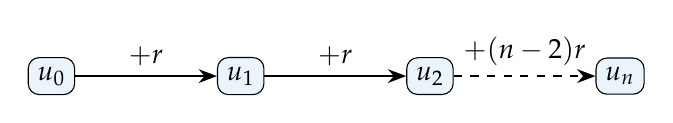
\begin{tikzpicture}[>=Stealth,node distance=18mm]
\node[draw,rounded corners,fill=Sky] (u0) {$u_0$};
\node[draw,rounded corners,fill=Sky,right=of u0] (u1) {$u_1$};
\node[draw,rounded corners,fill=Sky,right=of u1] (u2) {$u_2$};
\node[draw,rounded corners,fill=Sky,right=of u2] (un) {$u_n$};
\draw[->,thick] (u0)--node[above] {$+r$}(u1);
\draw[->,thick] (u1)--node[above] {$+r$}(u2);
\draw[->,thick,dashed] (u2)--node[above] {$+(n-2)r$}(un);
\end{tikzpicture}
\end{center}

Three numbers $x,y,z$, written in this order, are three consecutive terms of an arithmetic sequence if $y-x=z-y$, that is, if $y=\dfrac{x+z}{2}$. This last quantity is the arithmetic mean of $x$ and $z$.

\begin{methode}
To model an additive situation: 1) define $u_n$ and state the unit; 2) identify the first term; 3) express the constant increase or decrease as the common difference $r$; 4) write the general term; 5) answer with a sentence in context.
\end{methode}

\begin{exemple}
A shop sells $480$ units in the first month and then $25$ more units each month. With $u_1=480$ and $r=25$, we get $u_n=480+25(n-1)$. Thus $u_{12}=755$: the shop expects to sell $755$ units in the twelfth month.
\end{exemple}

\subsection{Sum of arithmetic terms}
For the $n+1$ terms from $u_0$ to $u_n$,
\[
u_0+u_1+\cdots+u_n=(n+1)\frac{u_0+u_n}{2}.
\]
The formula is easy to remember as: \emph{number of terms multiplied by the mean of the first and last terms}.

\begin{erreur}
In $u_3+u_4+\cdots+u_{12}$, there are $12-3+1=10$ terms, not $9$ or $12$.
\end{erreur}

\subsection{Geometric sequence}
\begin{retenir}
A sequence $(u_n)$ is \textbf{geometric} when there is a real number $q$ such that $u_{n+1}=q u_n$. If the first term is $u_0$, then $u_n=u_0q^n$. If the first term is $u_1$, then $u_n=u_1q^{n-1}$.
\end{retenir}

\begin{center}
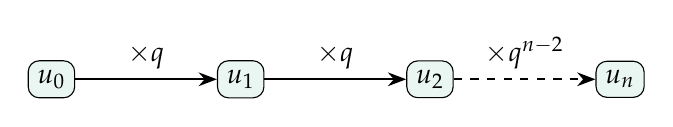
\begin{tikzpicture}[>=Stealth,node distance=18mm]
\node[draw,rounded corners,fill=Mint] (u0) {$u_0$};
\node[draw,rounded corners,fill=Mint,right=of u0] (u1) {$u_1$};
\node[draw,rounded corners,fill=Mint,right=of u1] (u2) {$u_2$};
\node[draw,rounded corners,fill=Mint,right=of u2] (un) {$u_n$};
\draw[->,thick] (u0)--node[above] {$\times q$}(u1);
\draw[->,thick] (u1)--node[above] {$\times q$}(u2);
\draw[->,thick,dashed] (u2)--node[above] {$\times q^{n-2}$}(un);
\end{tikzpicture}
\end{center}

An increase of $t\,\%$ corresponds to $q=1+\dfrac{t}{100}$; a decrease of $t\,\%$ to $q=1-\dfrac{t}{100}$. Three positive terms $x,y,z$ are consecutive in a geometric sequence if $y^2=xz$; $y=\sqrt{xz}$ is their geometric mean.

For $q\neq1$,
\[
u_0+u_1+\cdots+u_n=u_0\frac{1-q^{n+1}}{1-q}.
\]

\subsection{Algorithms: computing a sum}
\begin{lstlisting}[style=python]
def somme_carres(n):
    s = 0
    for k in range(1, n + 1):
        s = s + k**2
    return s
\end{lstlisting}
The accumulator \texttt{s} holds the partial sum; the counter \texttt{k} runs through the integers from $1$ to $n$.

\sessionheader{1}{15 Sep 2026}{B: 2 h -- C: 1 h}{Arithmetic sequences: recognising and modelling}{Number Sequences}
    \begin{objectifs}\begin{itemize}\item Recognise an additive change.\item Find the common difference.\item Define a sequence in context.\end{itemize}\end{objectifs}
    \begin{automatismes}\begin{enumerate}\item Write the multiplier for a $10\,\%$ increase. \rep{$1+\dfrac{10}{100}=1.10$}\item Calculate $u_4$ if $u_0=14$ and $u_{n+1}=u_n+3$. \rep{$u_4=26$}\item How many terms from $u_3$ to $u_{15}$? \rep{$15-3+1=13$}\item Give the multiplier for a $8\,\%$ decrease. \rep{$0.92$}\item Give the common difference of $12,12+4,12+2\times4,\ldots$. \rep{$r=4$}\end{enumerate}\end{automatismes}
    \begin{prerequis}Reread the last written record and be able to carry out the basic calculations needed today. Before the investigation, have the key words rephrased: recognise an additive change and find the common difference.\end{prerequis}

    \begin{activite}
    A club has $320$ members. It expects to gain $18$ more each year. Let $u_n$ be the number of members after $n$ years. Calculate $u_0,u_1,u_2$. Which operation takes you from one term to the next? Write a relation between $u_{n+1}$ and $u_n$, then predict $u_5$.
    \begin{center}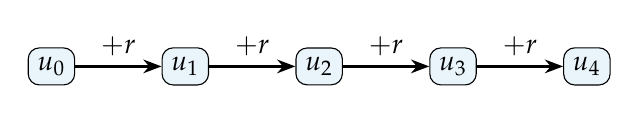
\begin{tikzpicture}[>=Stealth,node distance=17mm]
\foreach \i in {0,...,4}{\node[draw,rounded corners,fill=Sky] (u\i) at (1.7*\i,0) {$u_\i$};}
\foreach \i [evaluate=\i as \j using int(\i+1)] in {0,...,3}{\draw[->,thick] (u\i)--node[above] {$ +r $}(u\j);}
\end{tikzpicture}\end{center}
    \end{activite}
    \enseignant{$u_0=320$, $u_1=338$, $u_2=356$; we add $18$. So $u_{n+1}=u_n+18$ and $u_5=410$. Have students say aloud which piece of data triggers the choice of method.}

    \begin{traceecrite}A sequence is arithmetic when $u_{n+1}-u_n=r$ is constant. In a real-life situation, a constant absolute increase leads to an arithmetic sequence.\end{traceecrite}

    \begin{exemple}
    Take the data from the investigation and write up the solution in this order: definition of the objects, property used, exact or approximate calculation, then a sentence giving the answer. The model answer appears in the teacher edition.
    \end{exemple}
    \enseignant{$u_0=320$, $u_1=338$, $u_2=356$; we add $18$. So $u_{n+1}=u_n+18$ and $u_5=410$.}

    \begin{exercice}[-- essential]
    \begin{enumerate}\item The sequence $(u_n)$ satisfies $u_0=110$ et $u_{n+1}=u_n+3$. Write $u_n$ then calculate $u_{12}$.\item A quantity is worth $420$ and decreases by $3\,\%$ per period. Write $v_n$ and calculate $v_5$.\item For each sequence, say whether the model is arithmetic or geometric and justify it with a difference or a quotient.\end{enumerate}
    \end{exercice}
    \enseignant{$u_n=110+3n$ et $u_{12}=146$, for the second one, $q=0.97$ et $v_n=420\times q^n$; the third item is justified by the constant difference or quotient,}

    \manuelref{Calao, course notes pp. 18--21; exercises p. 24, no.~1--3}
\ExoSession{1}

    \begin{dm}Redo practice exercise 2 with the following data: replace the initial value by $125$ and the rate or common difference/ratio by $3$. Write it up in four lines: data, formula, calculation, conclusion.\end{dm}
    \enseignant{The correction depends on the exercise redone. Check above all the consistency of the model, the number of iterations, the rounding and the concluding sentence.}

    \begin{sortie}On a half-sheet: write the main rule of the session, work through a very short example and give your confidence level from 1 to 4. Key question(s) of the day: 1, 2 and 3.\end{sortie}

    \ifprof
    \begin{methode}
    \textbf{Running a 1-hour session:} 7 min of fluency; 10 min of sharing and written record; 28 min of essential exercises; 5 min of correction; 3 min of exit ticket.\\
    \textbf{Running a 2-hour session:} add 20 min of investigation, 20 min of formalising the rule, a second independent exercise and 10 min of comparative correction.\\
    \textbf{Differentiation:} give struggling students a four-box sheet (data, model, calculation, conclusion). Ask fast finishers to produce a counterexample, a justification or a second method.
    \end{methode}
    \fi
\sessionheader{2}{17 Sep 2026}{B: 1 h -- C: 2 h}{Arithmetic sequences: the general term}{Number Sequences}
\begin{objectifs}\begin{itemize}\item Move from the recurrence relation to the general term.\item Calculate a distant term.\item Interpret the index.\end{itemize}\end{objectifs}
\begin{automatismes}\begin{enumerate}\item Simplify $3x+5-x+2$. \rep{$2x+7$}\item How many terms from $u_3$ to $u_{15}$? \rep{$15-3+1=13$}\item Give the multiplier for a $8\,\%$ decrease. \rep{$0.92$}\item Give the common difference of $12,12+5,12+2\times5,\ldots$. \rep{$r=5$}\item Calculate $u_4$ if $u_0=15$ and $u_{n+1}=u_n+3$. \rep{$u_4=27$}\end{enumerate}\end{automatismes}
\begin{prerequis}Reread the last written record and be able to carry out the basic calculations needed today. Before the investigation, have the key words rephrased: move from the recurrence relation to the general term and calculate a distant term.\end{prerequis}

\begin{activite}
A shop has $1\,250$ active loyalty cards at index $0$ and gains $75$ per month. Without calculating all the terms, find the number of cards at index $n$, then at index $18$. Explain the role of $18$ in the calculation.

\end{activite}
\enseignant{$u_n=1\,250+75n$, so $u_{18}=2\,600$. The number $18$ counts the increases since index $0$. Have students say aloud which piece of data triggers the choice of method.}

\begin{traceecrite}If $(u_n)$ is arithmetic with common difference $r$, then $u_n=u_0+nr$ or $u_n=u_1+(n-1)r$, depending on the index of the first term.\end{traceecrite}

\begin{exemple}
Take the data from the investigation and write up the solution in this order: definition of the objects, property used, exact or approximate calculation, then a sentence giving the answer. The model answer appears in the teacher edition.
\end{exemple}
\enseignant{$u_n=1\,250+75n$, so $u_{18}=2\,600$. The number $18$ counts the increases since index $0$.}

\begin{exercice}[-- essential]
\begin{enumerate}\item The sequence $(u_n)$ satisfies $u_0=120$ et $u_{n+1}=u_n+4$. Write $u_n$ then calculate $u_{12}$.\item A quantity is worth $440$ and decreases by $4\,\%$ per period. Write $v_n$ and calculate $v_5$.\item For each sequence, say whether the model is arithmetic or geometric and justify it with a difference or a quotient.\end{enumerate}
\end{exercice}
\enseignant{$u_n=120+4n$ et $u_{12}=168$, for the second one, $q=0.96$ et $v_n=440\times q^n$; the third item is justified by the constant difference or quotient,}

\manuelref{Calao, course notes pp. 18--21; exercises p. 24, no.~5--8}
\ExoSession{2}

\begin{dm}Redo practice exercise 3 with the following data: replace the initial value by $130$ and the rate or common difference/ratio by $4$. Write it up in four lines: data, formula, calculation, conclusion.\end{dm}
\enseignant{The correction depends on the exercise redone. Check above all the consistency of the model, the number of iterations, the rounding and the concluding sentence.}

\begin{sortie}On a half-sheet: write the main rule of the session, work through a very short example and give your confidence level from 1 to 4. Key question(s) of the day: 1 and 2.\end{sortie}

\ifprof
\begin{methode}
\textbf{Running a 1-hour session:} 7 min of fluency; 10 min of sharing and written record; 28 min of essential exercises; 5 min of correction; 3 min of exit ticket.\\
\textbf{Running a 2-hour session:} add 20 min of investigation, 20 min of formalising the rule, a second independent exercise and 10 min of comparative correction.\\
\textbf{Differentiation:} give struggling students a four-box sheet (data, model, calculation, conclusion). Ask fast finishers to produce a counterexample, a justification or a second method.
\end{methode}
\fi
\sessionheader{3}{22 Sep 2026}{B: 2 h -- C: 1 h}{Sum of the terms of an arithmetic sequence}{Number Sequences}
\begin{objectifs}\begin{itemize}\item Count the terms of a sum.\item Apply the formula.\item Check the order of magnitude.\end{itemize}\end{objectifs}
\begin{automatismes}\begin{enumerate}\item Calculate $20\,\%$ of $120$. \rep{$24$}\item Give the multiplier for a $8\,\%$ decrease. \rep{$0.92$}\item Give the common difference of $12,12+6,12+2\times6,\ldots$. \rep{$r=6$}\item Calculate $u_4$ if $u_0=16$ and $u_{n+1}=u_n+3$. \rep{$u_4=28$}\item How many terms from $u_3$ to $u_{15}$? \rep{$15-3+1=13$}\end{enumerate}\end{automatismes}
\begin{prerequis}Reread the last written record and be able to carry out the basic calculations needed today. Before the investigation, have the key words rephrased: count the terms of a sum and apply the formula.\end{prerequis}

\begin{activite}
A company pays a monthly bonus: $45$ euros in the first month, then $5$ euros more each month. Calculate the total paid over the first twelve months in three ways: explicit sum, pairing first and last terms, formula.

\end{activite}
\enseignant{$u_{12}=45+11\times5=100$. The total is $12\times\dfrac{45+100}{2}=870$ euros. Have students say aloud which piece of data triggers the choice of method.}

\begin{traceecrite}A sum of arithmetic terms equals $\text{number of terms}\times\dfrac{\text{first}+\text{last}}2$. From $u_p$ to $u_q$, there are $q-p+1$ terms.\end{traceecrite}

\begin{exemple}
Take the data from the investigation and write up the solution in this order: definition of the objects, property used, exact or approximate calculation, then a sentence giving the answer. The model answer appears in the teacher edition.
\end{exemple}
\enseignant{$u_{12}=45+11\times5=100$. The total is $12\times\dfrac{45+100}{2}=870$ euros.}

\begin{exercice}[-- essential]
\begin{enumerate}\item The sequence $(u_n)$ satisfies $u_0=130$ et $u_{n+1}=u_n+5$. Write $u_n$ then calculate $u_{12}$.\item A quantity is worth $460$ and decreases by $5\,\%$ per period. Write $v_n$ and calculate $v_5$.\item For each sequence, say whether the model is arithmetic or geometric and justify it with a difference or a quotient.\end{enumerate}
\end{exercice}
\enseignant{$u_n=130+5n$ et $u_{12}=190$, for the second one, $q=0.95$ et $v_n=460\times q^n$; the third item is justified by the constant difference or quotient,}

\manuelref{Calao, course notes pp. 20--21; exercises p. 24, no.~11--13, then p. 28, no.~43--44}
\ExoSession{3}

\begin{dm}Redo practice exercise 2 with the following data: replace the initial value by $135$ and the rate or common difference/ratio by $5$. Write it up in four lines: data, formula, calculation, conclusion.\end{dm}
\enseignant{The correction depends on the exercise redone. Check above all the consistency of the model, the number of iterations, the rounding and the concluding sentence.}

\begin{sortie}On a half-sheet: write the main rule of the session, work through a very short example and give your confidence level from 1 to 4. Key question(s) of the day: 1, 2 and 3.\end{sortie}

\ifprof
\begin{methode}
\textbf{Running a 1-hour session:} 7 min of fluency; 10 min of sharing and written record; 28 min of essential exercises; 5 min of correction; 3 min of exit ticket.\\
\textbf{Running a 2-hour session:} add 20 min of investigation, 20 min of formalising the rule, a second independent exercise and 10 min of comparative correction.\\
\textbf{Differentiation:} give struggling students a four-box sheet (data, model, calculation, conclusion). Ask fast finishers to produce a counterexample, a justification or a second method.
\end{methode}
\fi
\sessionheader{4}{24 Sep 2026}{B: 1 h -- C: 2 h}{Geometric sequences: recognising and modelling}{Number Sequences}
    \begin{objectifs}\begin{itemize}\item Recognise a multiplicative change.\item Convert a rate into a multiplier.\item Compare arithmetic and geometric sequences.\end{itemize}\end{objectifs}
    \begin{automatismes}\begin{enumerate}\item Write the multiplier for a $25\,\%$ increase. \rep{$1+\dfrac{25}{100}=1.25$}\item Give the common difference of $12,12+7,12+2\times7,\ldots$. \rep{$r=7$}\item Calculate $u_4$ if $u_0=17$ and $u_{n+1}=u_n+3$. \rep{$u_4=29$}\item How many terms from $u_3$ to $u_{15}$? \rep{$15-3+1=13$}\item Give the multiplier for a $8\,\%$ decrease. \rep{$0.92$}\end{enumerate}\end{automatismes}
    \begin{prerequis}Reread the last written record and be able to carry out the basic calculations needed today. Before the investigation, have the key words rephrased: recognise a multiplicative change and convert a rate into a multiplier.\end{prerequis}

    \begin{activite}
    An online shop increases its number of visitors by $6\,\%$ per month, starting from $8\,000$ visitors. Calculate the first three values. Compare the differences, then the quotients. Identify the type of sequence.
    \begin{center}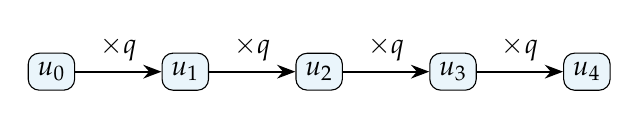
\begin{tikzpicture}[>=Stealth,node distance=17mm]
\foreach \i in {0,...,4}{\node[draw,rounded corners,fill=Sky] (u\i) at (1.7*\i,0) {$u_\i$};}
\foreach \i [evaluate=\i as \j using int(\i+1)] in {0,...,3}{\draw[->,thick] (u\i)--node[above] {$ \times q $}(u\j);}
\end{tikzpicture}\end{center}
    \end{activite}
    \enseignant{The multiplier is $1.06$: $8\,000$, $8\,480$, $8\,988.8$. The quotients are $1.06$; the sequence is geometric. Have students say aloud which piece of data triggers the choice of method.}

    \begin{traceecrite}A sequence is geometric when $\dfrac{u_{n+1}}{u_n}=q$ is constant (non-zero terms). A constant relative change leads to a geometric sequence.\end{traceecrite}

    \begin{exemple}
    Take the data from the investigation and write up the solution in this order: definition of the objects, property used, exact or approximate calculation, then a sentence giving the answer. The model answer appears in the teacher edition.
    \end{exemple}
    \enseignant{The multiplier is $1.06$: $8\,000$, $8\,480$, $8\,988.8$. The quotients are $1.06$; the sequence is geometric.}

    \begin{exercice}[-- essential]
    \begin{enumerate}\item The sequence $(u_n)$ satisfies $u_0=140$ et $u_{n+1}=u_n+6$. Write $u_n$ then calculate $u_{12}$.\item A quantity is worth $480$ and decreases by $6\,\%$ per period. Write $v_n$ and calculate $v_5$.\item For each sequence, say whether the model is arithmetic or geometric and justify it with a difference or a quotient.\end{enumerate}
    \end{exercice}
    \enseignant{$u_n=140+6n$ et $u_{12}=212$, for the second one, $q=0.94$ et $v_n=480\times q^n$; the third item is justified by the constant difference or quotient,}

    \manuelref{Calao, course notes pp. 23--25; exercises p. 25, no.~14--18}
\ExoSession{4}

    \begin{dm}Redo practice exercise 3 with the following data: replace the initial value by $140$ and the rate or common difference/ratio by $6$. Write it up in four lines: data, formula, calculation, conclusion.\end{dm}
    \enseignant{The correction depends on the exercise redone. Check above all the consistency of the model, the number of iterations, the rounding and the concluding sentence.}

    \begin{sortie}On a half-sheet: write the main rule of the session, work through a very short example and give your confidence level from 1 to 4. Key question(s) of the day: 1 and 2.\end{sortie}

    \ifprof
    \begin{methode}
    \textbf{Running a 1-hour session:} 7 min of fluency; 10 min of sharing and written record; 28 min of essential exercises; 5 min of correction; 3 min of exit ticket.\\
    \textbf{Running a 2-hour session:} add 20 min of investigation, 20 min of formalising the rule, a second independent exercise and 10 min of comparative correction.\\
    \textbf{Differentiation:} give struggling students a four-box sheet (data, model, calculation, conclusion). Ask fast finishers to produce a counterexample, a justification or a second method.
    \end{methode}
    \fi
\sessionheader{5}{29 Sep 2026}{B: 2 h -- C: 1 h}{Geometric sequences: general term and sum}{Number Sequences}
\begin{objectifs}\begin{itemize}\item Write the general term.\item Calculate a geometric sum.\item Interpret a cumulative change.\end{itemize}\end{objectifs}
\begin{automatismes}\begin{enumerate}\item Simplify $3x+8-x+2$. \rep{$2x+10$}\item Calculate $u_4$ if $u_0=18$ and $u_{n+1}=u_n+3$. \rep{$u_4=30$}\item How many terms from $u_3$ to $u_{15}$? \rep{$15-3+1=13$}\item Give the multiplier for a $8\,\%$ decrease. \rep{$0.92$}\item Give the common difference of $12,12+8,12+2\times8,\ldots$. \rep{$r=8$}\end{enumerate}\end{automatismes}
\begin{prerequis}Reread the last written record and be able to carry out the basic calculations needed today. Before the investigation, have the key words rephrased: write the general term and calculate a geometric sum.\end{prerequis}

\begin{activite}
A capital of $250\,000$ Ar is invested at $4\,\%$ per year, compound interest. Write the capital $C_n$ after $n$ years. Calculate $C_6$, then the sum $C_0+\cdots+C_6$, and explain what this last sum represents mathematically and why it is not the final capital.

\end{activite}
\enseignant{$C_n=250\,000\times1.04^n$ and $C_6\approx316\,330$ Ar. The sum is the sum of seven successive values, not an actual accumulation of the investment. Have students say aloud which piece of data triggers the choice of method.}

\begin{traceecrite}If $(u_n)$ is geometric with common ratio $q$, $u_n=u_0q^n$ ou $u_n=u_1q^{n-1}$. For $q\neq1$, $u_0+\cdots+u_n=u_0\dfrac{1-q^{n+1}}{1-q}$.\end{traceecrite}

\begin{exemple}
Take the data from the investigation and write up the solution in this order: definition of the objects, property used, exact or approximate calculation, then a sentence giving the answer. The model answer appears in the teacher edition.
\end{exemple}
\enseignant{$C_n=250\,000\times1.04^n$ and $C_6\approx316\,330$ Ar. The sum is the sum of seven successive values, not an actual accumulation of the investment.}

\begin{exercice}[-- essential]
\begin{enumerate}\item The sequence $(u_n)$ satisfies $u_0=150$ et $u_{n+1}=u_n+2$. Write $u_n$ then calculate $u_{12}$.\item A quantity is worth $500$ and decreases by $2\,\%$ per period. Write $v_n$ and calculate $v_5$.\item For each sequence, say whether the model is arithmetic or geometric and justify it with a difference or a quotient.\end{enumerate}
\end{exercice}
\enseignant{$u_n=150+2n$ et $u_{12}=174$, for the second one, $q=0.98$ et $v_n=500\times q^n$; the third item is justified by the constant difference or quotient,}

\manuelref{Calao, course notes pp. 25--28; exercises p. 25, no.~19--25, then p. 28, no.~42--44}
\ExoSession{5}

\begin{dm}Redo practice exercise 2 with the following data: replace the initial value by $145$ and the rate or common difference/ratio by $7$. Write it up in four lines: data, formula, calculation, conclusion.\end{dm}
\enseignant{The correction depends on the exercise redone. Check above all the consistency of the model, the number of iterations, the rounding and the concluding sentence.}

\begin{sortie}On a half-sheet: write the main rule of the session, work through a very short example and give your confidence level from 1 to 4. Key question(s) of the day: 1, 2 and 3.\end{sortie}

\ifprof
\begin{methode}
\textbf{Running a 1-hour session:} 7 min of fluency; 10 min of sharing and written record; 28 min of essential exercises; 5 min of correction; 3 min of exit ticket.\\
\textbf{Running a 2-hour session:} add 20 min of investigation, 20 min of formalising the rule, a second independent exercise and 10 min of comparative correction.\\
\textbf{Differentiation:} give struggling students a four-box sheet (data, model, calculation, conclusion). Ask fast finishers to produce a counterexample, a justification or a second method.
\end{methode}
\fi
\sessionheader{6}{1 Oct 2026}{B: 1 h -- C: 2 h}{Review and formative assessment}{Number Sequences}
\begin{objectifs}\begin{itemize}\item Choose the right model.\item Use the formulas.\item Analyse one's own mistakes.\end{itemize}\end{objectifs}
\begin{automatismes}\begin{enumerate}\item Calculate $5\,\%$ of $180$. \rep{$9$}\item How many terms from $u_3$ to $u_{15}$? \rep{$15-3+1=13$}\item Give the multiplier for a $8\,\%$ decrease. \rep{$0.92$}\item Give the common difference of $12,12+9,12+2\times9,\ldots$. \rep{$r=9$}\item Calculate $u_4$ if $u_0=19$ and $u_{n+1}=u_n+3$. \rep{$u_4=31$}\end{enumerate}\end{automatismes}
\begin{prerequis}Reread the last written record and be able to carry out the basic calculations needed today. Before the investigation, have the key words rephrased: choose the right model and use the formulas.\end{prerequis}

\begin{activite}
Sort eight situations into three categories: arithmetic, geometric, neither. For each situation, underline the word or piece of data that justifies the choice, then choose the appropriate formula.

\end{activite}
\enseignant{A constant absolute change indicates the arithmetic model; a constant percentage or multiplier indicates the geometric model; otherwise neither is guaranteed. Have students say aloud which piece of data triggers the choice of method.}

\begin{traceecrite}Before calculating, identify: type of sequence, first index, common difference or ratio, and the term or sum asked for. The conclusion states the unit and the index.\end{traceecrite}

\begin{exemple}
Take the data from the investigation and write up the solution in this order: definition of the objects, property used, exact or approximate calculation, then a sentence giving the answer. The model answer appears in the teacher edition.
\end{exemple}
\enseignant{A constant absolute change indicates the arithmetic model; a constant percentage or multiplier indicates the geometric model; otherwise neither is guaranteed.}

\begin{exercice}[-- essential]
\begin{enumerate}\item The sequence $(u_n)$ satisfies $u_0=160$ et $u_{n+1}=u_n+3$. Write $u_n$ then calculate $u_{12}$.\item A quantity is worth $520$ and decreases by $3\,\%$ per period. Write $v_n$ and calculate $v_5$.\item For each sequence, say whether the model is arithmetic or geometric and justify it with a difference or a quotient.\end{enumerate}
\end{exercice}
\enseignant{$u_n=160+3n$ et $u_{12}=196$, for the second one, $q=0.97$ et $v_n=520\times q^n$; the third item is justified by the constant difference or quotient,}

\manuelref{Calao, p. 29, no.~49--52}
\ExoSession{6}

\begin{dm}Redo practice exercise 3 with the following data: replace the initial value by $150$ and the rate or common difference/ratio by $2$. Write it up in four lines: data, formula, calculation, conclusion.\end{dm}
\enseignant{The correction depends on the exercise redone. Check above all the consistency of the model, the number of iterations, the rounding and the concluding sentence.}

\begin{sortie}On a half-sheet: write the main rule of the session, work through a very short example and give your confidence level from 1 to 4. Key question(s) of the day: 1 and 2.\end{sortie}

\ifprof
\begin{methode}
\textbf{Running a 1-hour session:} 7 min of fluency; 10 min of sharing and written record; 28 min of essential exercises; 5 min of correction; 3 min of exit ticket.\\
\textbf{Running a 2-hour session:} add 20 min of investigation, 20 min of formalising the rule, a second independent exercise and 10 min of comparative correction.\\
\textbf{Differentiation:} give struggling students a four-box sheet (data, model, calculation, conclusion). Ask fast finishers to produce a counterexample, a justification or a second method.
\end{methode}
\fi


\chapter{Exponential Functions}
\competences{model a continuous change, switch between representations, calculate, interpret}
\section{Core Course Notes}
For $a>0$, the function $x\mapsto a^x$ extends the integer powers of $a$ to all real numbers. It satisfies $a^0=1$ and $a^{-x}=\dfrac{1}{a^x}$.

\begin{center}
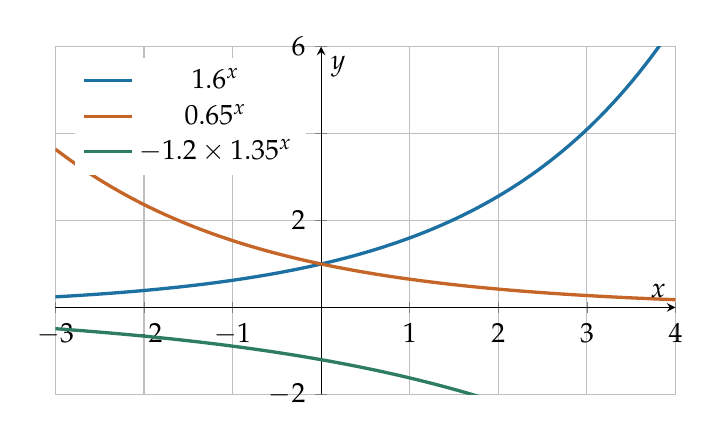
\begin{tikzpicture}
\begin{axis}[width=.78\textwidth,height=6cm,axis lines=middle,xmin=-3,xmax=4,ymin=-2,ymax=6,grid=major,xlabel={$x$},ylabel={$y$},legend style={at={(.03,.97)},anchor=north west,draw=none,fill=white}]
\addplot[Blue,very thick,samples=100,domain=-3:4]{1.6^x};\addlegendentry{$1.6^x$}
\addplot[Orange,very thick,samples=100,domain=-3:4]{0.65^x};\addlegendentry{$0.65^x$}
\addplot[Green,very thick,samples=100,domain=-3:4]{-1.2*1.35^x};\addlegendentry{$-1.2\times1.35^x$}
\end{axis}
\end{tikzpicture}
\end{center}

\begin{retenir}
If $a>1$, $x\mapsto a^x$ is strictly increasing. If $0<a<1$, it is strictly decreasing. For $f(x)=ka^x$, multiplying by $k<0$ reverses the direction of variation. In every case, $a^x>0$.
\end{retenir}

For $a>0$ and all real numbers $x,y$:
\[
a^{x+y}=a^xa^y,\qquad a^{x-y}=\frac{a^x}{a^y},\qquad (a^x)^y=a^{xy}.
\]

\begin{erreur}
In general, $a^x+a^y\neq a^{x+y}$. The rules apply to products and quotients, not to sums.
\end{erreur}

\subsection{Changes and average rate}
A quantity with initial value $V_0$ undergoing a constant relative change with multiplier $q$ is modelled by $V(t)=V_0q^t$. If an overall multiplier $Q$ results from $n$ identical changes, the average multiplier is $q=Q^{\frac1n}$ and the average rate is $t=q-1$.

\begin{exemple}
A company's turnover goes from $80\,000$ to $95\,000$ euros in four years. The overall multiplier is $Q=\dfrac{95\,000}{80\,000}=1.1875$. The average annual multiplier is $q=1.1875^{\frac14}\approx1.0440$: the average annual rate is therefore about $4.40\,\%$.
\end{exemple}

\subsection{Solving and interpreting}
When both sides can be written with the same base, we use injectivity: for $a>0$ and $a\neq1$, $a^u=a^v$ is equivalent to $u=v$. Otherwise, a graphical or numerical solution gives an approximate value; the common logarithm (base 10), studied later, will give a formula.

\sessionheader{7}{6 Oct 2026}{B: 2 h -- C: 1 h}{Definition and direction of variation of $a^x$}{Exponential Functions}
\begin{objectifs}\begin{itemize}\item Make sense of $a^x$.\item Link the base to the direction of variation.\item Read curves.\end{itemize}\end{objectifs}
\begin{automatismes}\begin{enumerate}\item Write the multiplier for a $10\,\%$ increase. \rep{$1+\dfrac{10}{100}=1.10$}\item Compare $1.04^3$ and $1.04^7$. \rep{$1.04^3<1.04^7$}\item Calculer $2^4\times2^3$. \rep{$2^7$}\item Write $5^{-2}$ as a fraction. \rep{$\dfrac1{25}$}\item Is the function $x\mapsto0.7^x$ increasing?? \rep{No, it is decreasing.}\end{enumerate}\end{automatismes}
\begin{prerequis}Reread the last written record and be able to carry out the basic calculations needed today. Before the investigation, have the key words rephrased: make sense of $a^x$ and link the base to the direction of variation.\end{prerequis}

\begin{activite}
Using a calculator, complete a table of values of $1.5^x$ and $0.7^x$ for $x=-2,-1,0,1,2,3$. Plot the points, conjecture the variations and identify the point common to both curves.
\begin{center}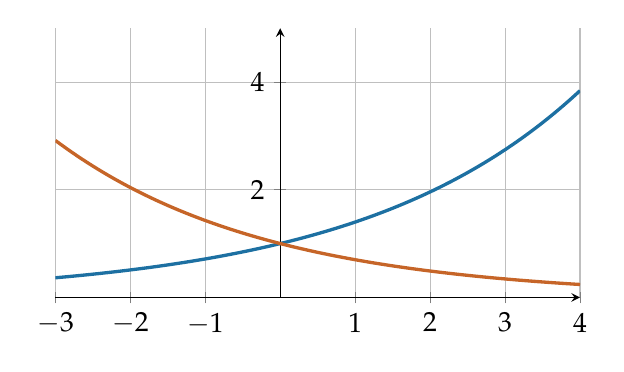
\begin{tikzpicture}\begin{axis}[width=.68\textwidth,height=5cm,axis lines=middle,xmin=-3,xmax=4,ymin=0,ymax=5,grid=major]\addplot[Blue,very thick,samples=100,domain=-3:4]{1.4^x};\addplot[Orange,very thick,samples=100,domain=-3:4]{.7^x};\end{axis}\end{tikzpicture}\end{center}
\end{activite}
\enseignant{$a^0=1$, so the curves pass through $(0,1)$. The first increases and the second decreases. Have students say aloud which piece of data triggers the choice of method.}

\begin{traceecrite}For $a>0$, $a^x$ is defined for every real number $x$. The function is increasing if $a>1$ and decreasing if $0<a<1$.\end{traceecrite}

\begin{exemple}
Take the data from the investigation and write up the solution in this order: definition of the objects, property used, exact or approximate calculation, then a sentence giving the answer. The model answer appears in the teacher edition.
\end{exemple}
\enseignant{$a^0=1$, so the curves pass through $(0,1)$. The first increases and the second decreases.}

\begin{exercice}[-- essential]
\begin{enumerate}\item Simplify $3^{x+4}\div3^x$ and $(2^x)^3$.\item Study the direction of variation of $f(x)=4\times1.04^x$ and $g(x)=-4\times0.8^x$.\item An initial value of $1350$ increases by $4\,\%$ per year. Give the model and calculate the value after $6$ years.\end{enumerate}
\end{exercice}
\enseignant{$3^4$ et $2^{3x}$. $f$ is increasing; $0.8^x$ is decreasing and the negative coefficient makes $g$ increasing. The model is $V(t)=1350\times\left(1+\dfrac{4}{100}\right)^t$.}

\manuelref{Calao, course notes pp. 42--47; exercises p. 48, no.~1--8}
\ExoSession{7}

\begin{dm}Redo practice exercise 2 with the following data: replace the initial value by $155$ and the rate or common difference/ratio by $3$. Write it up in four lines: data, formula, calculation, conclusion.\end{dm}
\enseignant{The correction depends on the exercise redone. Check above all the consistency of the model, the number of iterations, the rounding and the concluding sentence.}

\begin{sortie}On a half-sheet: write the main rule of the session, work through a very short example and give your confidence level from 1 to 4. Key question(s) of the day: 1, 2 and 3.\end{sortie}

\ifprof
\begin{methode}
\textbf{Running a 1-hour session:} 7 min of fluency; 10 min of sharing and written record; 28 min of essential exercises; 5 min of correction; 3 min of exit ticket.\\
\textbf{Running a 2-hour session:} add 20 min of investigation, 20 min of formalising the rule, a second independent exercise and 10 min of comparative correction.\\
\textbf{Differentiation:} give struggling students a four-box sheet (data, model, calculation, conclusion). Ask fast finishers to produce a counterexample, a justification or a second method.
\end{methode}
\fi
\sessionheader{8}{8 Oct 2026}{B: 1 h -- C: 2 h}{Powers and algebraic rules}{Exponential Functions}
\begin{objectifs}\begin{itemize}\item Transform powers.\item Use negative exponents.\item Spot a rule that does not apply.\end{itemize}\end{objectifs}
\begin{automatismes}\begin{enumerate}\item Simplify $3x+4-x+2$. \rep{$2x+6$}\item Calculer $2^1\times2^3$. \rep{$2^4$}\item Write $5^{-2}$ as a fraction. \rep{$\dfrac1{25}$}\item Is the function $x\mapsto0.7^x$ increasing?? \rep{No, it is decreasing.}\item Compare $1.04^3$ and $1.04^7$. \rep{$1.04^3<1.04^7$}\end{enumerate}\end{automatismes}
\begin{prerequis}Reread the last written record and be able to carry out the basic calculations needed today. Before the investigation, have the key words rephrased: transform powers and use negative exponents.\end{prerequis}

\begin{activite}
Simplify $2^3\times2^{-5}$, $5^{x+2}\div5^x$ and $(3^x)^2$. Then invent a numerical counterexample to $a^x+a^y=a^{x+y}$.

\end{activite}
\enseignant{We get $2^{-2}=\dfrac14$, $5^2=25$ and $3^{2x}$. With $a=2,x=y=1$, $2+2\neq4$? Here the equality holds by accident; choose $a=3$: $3+3\neq9$. Have students say aloud which piece of data triggers the choice of method.}

\begin{traceecrite}$a^{x+y}=a^xa^y$, $a^{x-y}=\dfrac{a^x}{a^y}$ et $(a^x)^y=a^{xy}$. These rules require the same positive base.\end{traceecrite}

\begin{exemple}
Take the data from the investigation and write up the solution in this order: definition of the objects, property used, exact or approximate calculation, then a sentence giving the answer. The model answer appears in the teacher edition.
\end{exemple}
\enseignant{We get $2^{-2}=\dfrac14$, $5^2=25$ and $3^{2x}$. With $a=2,x=y=1$, $2+2\neq4$? Here the equality holds by accident; choose $a=3$: $3+3\neq9$.}

\begin{exercice}[-- essential]
\begin{enumerate}\item Simplify $3^{x+5}\div3^x$ and $(2^x)^3$.\item Study the direction of variation of $f(x)=5\times1.05^x$ and $g(x)=-5\times0.8^x$.\item An initial value of $1400$ increases by $5\,\%$ per year. Give the model and calculate the value after $6$ years.\end{enumerate}
\end{exercice}
\enseignant{$3^5$ et $2^{3x}$. $f$ is increasing; $0.8^x$ is decreasing and the negative coefficient makes $g$ increasing. The model is $V(t)=1400\times\left(1+\dfrac{5}{100}\right)^t$.}

\manuelref{Calao, course notes pp. 43--45; exercises p. 49, no.~9--13}
\ExoSession{8}

\begin{dm}Redo practice exercise 3 with the following data: replace the initial value by $160$ and the rate or common difference/ratio by $4$. Write it up in four lines: data, formula, calculation, conclusion.\end{dm}
\enseignant{The correction depends on the exercise redone. Check above all the consistency of the model, the number of iterations, the rounding and the concluding sentence.}

\begin{sortie}On a half-sheet: write the main rule of the session, work through a very short example and give your confidence level from 1 to 4. Key question(s) of the day: 1 and 2.\end{sortie}

\ifprof
\begin{methode}
\textbf{Running a 1-hour session:} 7 min of fluency; 10 min of sharing and written record; 28 min of essential exercises; 5 min of correction; 3 min of exit ticket.\\
\textbf{Running a 2-hour session:} add 20 min of investigation, 20 min of formalising the rule, a second independent exercise and 10 min of comparative correction.\\
\textbf{Differentiation:} give struggling students a four-box sheet (data, model, calculation, conclusion). Ask fast finishers to produce a counterexample, a justification or a second method.
\end{methode}
\fi
\sessionheader{9}{13 Oct 2026}{B: 2 h -- C: 1 h}{Functions $x\mapsto k a^x$: variation and graph}{Exponential Functions}
\begin{objectifs}\begin{itemize}\item Study $ka^x$.\item Combine sign and variation.\item Link formula and graph.\end{itemize}\end{objectifs}
\begin{automatismes}\begin{enumerate}\item Calculate $20\,\%$ of $100$. \rep{$20$}\item Write $5^{-2}$ as a fraction. \rep{$\dfrac1{25}$}\item Is the function $x\mapsto0.7^x$ increasing?? \rep{No, it is decreasing.}\item Compare $1.04^3$ and $1.04^7$. \rep{$1.04^3<1.04^7$}\item Calculer $2^2\times2^3$. \rep{$2^5$}\end{enumerate}\end{automatismes}
\begin{prerequis}Reread the last written record and be able to carry out the basic calculations needed today. Before the investigation, have the key words rephrased: study $ka^x$ and combine sign and variation.\end{prerequis}

\begin{activite}
Match the four functions $2^x$, $0.6^x$, $-2^x$ and $-0.6^x$ to four curves. Justify each choice using the sign, the $y$-intercept and the direction of variation.
\begin{center}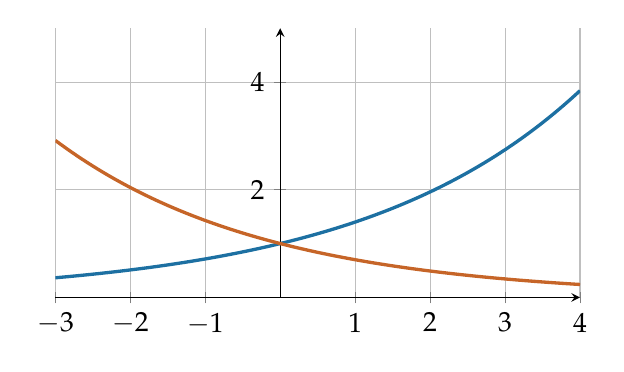
\begin{tikzpicture}\begin{axis}[width=.68\textwidth,height=5cm,axis lines=middle,xmin=-3,xmax=4,ymin=0,ymax=5,grid=major]\addplot[Blue,very thick,samples=100,domain=-3:4]{1.4^x};\addplot[Orange,very thick,samples=100,domain=-3:4]{.7^x};\end{axis}\end{tikzpicture}\end{center}
\end{activite}
\enseignant{All have absolute value $1$ at $0$. The sign distinguishes the two pairs; the base and the sign of the coefficient determine the variation. Have students say aloud which piece of data triggers the choice of method.}

\begin{traceecrite}For $f(x)=ka^x$, the sign is that of $k$. If $k<0$, multiplying by $k$ reverses the direction of variation of $a^x$.\end{traceecrite}

\begin{exemple}
Take the data from the investigation and write up the solution in this order: definition of the objects, property used, exact or approximate calculation, then a sentence giving the answer. The model answer appears in the teacher edition.
\end{exemple}
\enseignant{All have absolute value $1$ at $0$. The sign distinguishes the two pairs; the base and the sign of the coefficient determine the variation.}

\begin{exercice}[-- essential]
\begin{enumerate}\item Simplify $3^{x+6}\div3^x$ and $(2^x)^3$.\item Study the direction of variation of $f(x)=6\times1.06^x$ and $g(x)=-6\times0.8^x$.\item An initial value of $1450$ increases by $6\,\%$ per year. Give the model and calculate the value after $6$ years.\end{enumerate}
\end{exercice}
\enseignant{$3^6$ et $2^{3x}$. $f$ is increasing; $0.8^x$ is decreasing and the negative coefficient makes $g$ increasing. The model is $V(t)=1450\times\left(1+\dfrac{6}{100}\right)^t$.}

\manuelref{Calao, course notes pp. 44--47; exercises p. 48, no.~5--8, then p. 52, no.~31--36}
\ExoSession{9}

\begin{dm}Redo practice exercise 2 with the following data: replace the initial value by $165$ and the rate or common difference/ratio by $5$. Write it up in four lines: data, formula, calculation, conclusion.\end{dm}
\enseignant{The correction depends on the exercise redone. Check above all the consistency of the model, the number of iterations, the rounding and the concluding sentence.}

\begin{sortie}On a half-sheet: write the main rule of the session, work through a very short example and give your confidence level from 1 to 4. Key question(s) of the day: 1, 2 and 3.\end{sortie}

\ifprof
\begin{methode}
\textbf{Running a 1-hour session:} 7 min of fluency; 10 min of sharing and written record; 28 min of essential exercises; 5 min of correction; 3 min of exit ticket.\\
\textbf{Running a 2-hour session:} add 20 min of investigation, 20 min of formalising the rule, a second independent exercise and 10 min of comparative correction.\\
\textbf{Differentiation:} give struggling students a four-box sheet (data, model, calculation, conclusion). Ask fast finishers to produce a counterexample, a justification or a second method.
\end{methode}
\fi
\sessionheader{10}{15 Oct 2026}{B: 1 h -- C: 2 h}{Average rate of change}{Exponential Functions}
\begin{objectifs}\begin{itemize}\item Calculate an average rate.\item Distinguish overall and average rates.\item Interpret an exponent $\frac1n$.\end{itemize}\end{objectifs}
\begin{automatismes}\begin{enumerate}\item Write the multiplier for a $25\,\%$ increase. \rep{$1+\dfrac{25}{100}=1.25$}\item Is the function $x\mapsto0.7^x$ increasing?? \rep{No, it is decreasing.}\item Compare $1.04^3$ and $1.04^7$. \rep{$1.04^3<1.04^7$}\item Calculer $2^3\times2^3$. \rep{$2^6$}\item Write $5^{-2}$ as a fraction. \rep{$\dfrac1{25}$}\end{enumerate}\end{automatismes}
\begin{prerequis}Reread the last written record and be able to carry out the basic calculations needed today. Before the investigation, have the key words rephrased: calculate an average rate and distinguish overall and average rates.\end{prerequis}

\begin{activite}
The price of a service goes from $18$ to $23.50$ euros in five years. Calculate the overall multiplier, then the average annual multiplier and the average annual rate. Check by applying the change five times in a row.

\end{activite}
\enseignant{$Q=\dfrac{23.5}{18}\approx1.3056$, $q=Q^{\frac15}\approx1.0548$, that is, about $5.48\,\%$ per year. Have students say aloud which piece of data triggers the choice of method.}

\begin{traceecrite}If $Q$ is the overall multiplier of $n$ identical changes, the average multiplier is $q=Q^{\frac1n}$ and the average rate is $q-1$.\end{traceecrite}

\begin{exemple}
Take the data from the investigation and write up the solution in this order: definition of the objects, property used, exact or approximate calculation, then a sentence giving the answer. The model answer appears in the teacher edition.
\end{exemple}
\enseignant{$Q=\dfrac{23.5}{18}\approx1.3056$, $q=Q^{\frac15}\approx1.0548$, that is, about $5.48\,\%$ per year.}

\begin{exercice}[-- essential]
\begin{enumerate}\item Simplify $3^{x+2}\div3^x$ and $(2^x)^3$.\item Study the direction of variation of $f(x)=2\times1.02^x$ and $g(x)=-2\times0.8^x$.\item An initial value of $1500$ increases by $2\,\%$ per year. Give the model and calculate the value after $6$ years.\end{enumerate}
\end{exercice}
\enseignant{$3^2$ and $2^{3x}$. $f$ is increasing; $0.8^x$ is decreasing and the negative coefficient makes $g$ increasing. The model is $V(t)=1500\times\left(1+\dfrac{2}{100}\right)^t$.}

\manuelref{Calao, course notes pp. 47--49; exercises p. 49, no.~14--19, then p. 54, no.~47--50}
\ExoSession{10}

\begin{dm}Redo practice exercise 3 with the following data: replace the initial value by $170$ and the rate or common difference/ratio by $6$. Write it up in four lines: data, formula, calculation, conclusion.\end{dm}
\enseignant{The correction depends on the exercise redone. Check above all the consistency of the model, the number of iterations, the rounding and the concluding sentence.}

\begin{sortie}On a half-sheet: write the main rule of the session, work through a very short example and give your confidence level from 1 to 4. Key question(s) of the day: 1 and 2.\end{sortie}

\ifprof
\vspace{-12mm}\begin{methode}\footnotesize
\textbf{Running a 1-hour session:} 7 min of fluency; 10 min of sharing and written record; 28 min of essential exercises; 5 min of correction; 3 min of exit ticket.\\
\textbf{Running a 2-hour session:} add 20 min of investigation, 20 min of formalising the rule, a second independent exercise and 10 min of comparative correction.\\
\textbf{Differentiation:} four-box sheet (data, model, calculation, conclusion) for struggling students; a counterexample, a justification or a second method for fast finishers.
\end{methode}
\fi
\sessionheader{11}{3 Nov 2026}{B: 2 h -- C: 1 h}{Reading graphical representations}{Exponential Functions}
\begin{objectifs}\begin{itemize}\item Read outputs and find the inputs that give them.\item Compare two models.\item Estimate graphically.\end{itemize}\end{objectifs}
\begin{automatismes}\begin{enumerate}\item Simplify $3x+7-x+2$. \rep{$2x+9$}\item Compare $1.04^3$ and $1.04^7$. \rep{$1.04^3<1.04^7$}\item Calculer $2^4\times2^3$. \rep{$2^7$}\item Write $5^{-2}$ as a fraction. \rep{$\dfrac1{25}$}\item Is the function $x\mapsto0.7^x$ increasing?? \rep{No, it is decreasing.}\end{enumerate}\end{automatismes}
\begin{prerequis}Reread the last written record and be able to carry out the basic calculations needed today. Before the investigation, have the key words rephrased: read outputs and find the inputs that give them and compare two models.\end{prerequis}

\begin{activite}
Two commercial offers are modelled by $f(x)=120\times1.08^x$ and $g(x)=180\times0.96^x$. Draw the curves on $[0,12]$, read off their point of intersection and interpret the regions where each value is the greater.
\begin{center}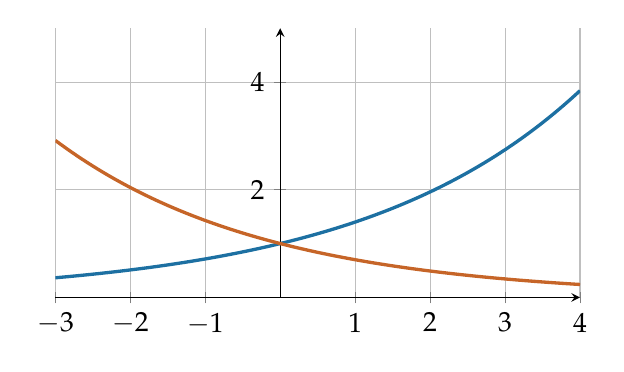
\begin{tikzpicture}\begin{axis}[width=.68\textwidth,height=5cm,axis lines=middle,xmin=-3,xmax=4,ymin=0,ymax=5,grid=major]\addplot[Blue,very thick,samples=100,domain=-3:4]{1.4^x};\addplot[Orange,very thick,samples=100,domain=-3:4]{.7^x};\end{axis}\end{tikzpicture}\end{center}
\end{activite}
\enseignant{The graph places the intersection near $x\approx3.5$. Before that point $g$ is greater; after it, $f$ is greater. An approximate value is expected. Have students say aloud which piece of data triggers the choice of method.}

\begin{traceecrite}Reading $f(x)$ means going from $x$ to the curve and then to the $y$-axis. Finding an input for a given $y$ means going from $y$ to the curve and then to the $x$-axis.\end{traceecrite}

\begin{exemple}
Take the data from the investigation and write up the solution in this order: definition of the objects, property used, exact or approximate calculation, then a sentence giving the answer. The model answer appears in the teacher edition.
\end{exemple}
\enseignant{The graph places the intersection near $x\approx3.5$. Before that point $g$ is greater; after it, $f$ is greater. An approximate value is expected.}

\begin{exercice}[-- essential]
\begin{enumerate}\item Simplify $3^{x+3}\div3^x$ and $(2^x)^3$.\item Study the direction of variation of $f(x)=3\times1.03^x$ and $g(x)=-3\times0.8^x$.\item An initial value of $1550$ increases by $3\,\%$ per year. Give the model and calculate the value after $6$ years.\end{enumerate}
\end{exercice}
\enseignant{$3^3$ et $2^{3x}$. $f$ is increasing; $0.8^x$ is decreasing and the negative coefficient makes $g$ increasing. The model is $V(t)=1550\times\left(1+\dfrac{3}{100}\right)^t$.}

\manuelref{Calao, p. 52, no.~31--36}
\ExoSession{11}

\begin{dm}Redo practice exercise 2 with the following data: replace the initial value by $175$ and the rate or common difference/ratio by $7$. Write it up in four lines: data, formula, calculation, conclusion.\end{dm}
\enseignant{The correction depends on the exercise redone. Check above all the consistency of the model, the number of iterations, the rounding and the concluding sentence.}

\begin{sortie}On a half-sheet: write the main rule of the session, work through a very short example and give your confidence level from 1 to 4. Key question(s) of the day: 1, 2 and 3.\end{sortie}

\ifprof
\begin{methode}
\textbf{Running a 1-hour session:} 7 min of fluency; 10 min of sharing and written record; 28 min of essential exercises; 5 min of correction; 3 min of exit ticket.\\
\textbf{Running a 2-hour session:} add 20 min of investigation, 20 min of formalising the rule, a second independent exercise and 10 min of comparative correction.\\
\textbf{Differentiation:} give struggling students a four-box sheet (data, model, calculation, conclusion). Ask fast finishers to produce a counterexample, a justification or a second method.
\end{methode}
\fi
\sessionheader{12}{5 Nov 2026}{B: 1 h -- C: 2 h}{Simple exponential equations}{Exponential Functions}
\begin{objectifs}\begin{itemize}\item Solve using a common base.\item Approximate a solution.\item Check plausibility.\end{itemize}\end{objectifs}
\begin{automatismes}\begin{enumerate}\item Calculate $5\,\%$ of $160$. \rep{$8$}\item Calculer $2^1\times2^3$. \rep{$2^4$}\item Write $5^{-2}$ as a fraction. \rep{$\dfrac1{25}$}\item Is the function $x\mapsto0.7^x$ increasing?? \rep{No, it is decreasing.}\item Compare $1.04^3$ and $1.04^7$. \rep{$1.04^3<1.04^7$}\end{enumerate}\end{automatismes}
\begin{prerequis}Reread the last written record and be able to carry out the basic calculations needed today. Before the investigation, have the key words rephrased: solve using a common base and approximate a solution.\end{prerequis}

\begin{activite}
Solve $4^x=64$, $9^x=\dfrac13$ and $1.12^x=2$: first using a common base when possible, then numerically for the last one. Bracket the last solution between two integers.

\end{activite}
\enseignant{$x=3$; $9^x=3^{-1}$ so $2x=-1$ and $x=-\dfrac12$; finally $x\approx6.12$, between $6$ and $7$. Have students say aloud which piece of data triggers the choice of method.}

\begin{traceecrite}To solve $a^x=b$: use a common base when possible; otherwise bracket the solution or use a numerical tool. Check that $b>0$.\end{traceecrite}

\begin{exemple}
Take the data from the investigation and write up the solution in this order: definition of the objects, property used, exact or approximate calculation, then a sentence giving the answer. The model answer appears in the teacher edition.
\end{exemple}
\enseignant{$x=3$; $9^x=3^{-1}$ so $2x=-1$ and $x=-\dfrac12$; finally $x\approx6.12$, between $6$ and $7$.}

\begin{exercice}[-- essential]
\begin{enumerate}\item Simplify $3^{x+4}\div3^x$ and $(2^x)^3$.\item Study the direction of variation of $f(x)=4\times1.04^x$ and $g(x)=-4\times0.8^x$.\item An initial value of $1600$ increases by $4\,\%$ per year. Give the model and calculate the value after $6$ years.\end{enumerate}
\end{exercice}
\enseignant{$3^4$ et $2^{3x}$. $f$ is increasing; $0.8^x$ is decreasing and the negative coefficient makes $g$ increasing. The model is $V(t)=1600\times\left(1+\dfrac{4}{100}\right)^t$.}

\manuelref{Calao, p. 52, no.~37--38, then p. 54, no.~45--46}
\ExoSession{12}

\begin{dm}Redo practice exercise 3 with the following data: replace the initial value by $180$ and the rate or common difference/ratio by $2$. Write it up in four lines: data, formula, calculation, conclusion.\end{dm}
\enseignant{The correction depends on the exercise redone. Check above all the consistency of the model, the number of iterations, the rounding and the concluding sentence.}

\begin{sortie}On a half-sheet: write the main rule of the session, work through a very short example and give your confidence level from 1 to 4. Key question(s) of the day: 1 and 2.\end{sortie}

\ifprof
\begin{methode}
\textbf{Running a 1-hour session:} 7 min of fluency; 10 min of sharing and written record; 28 min of essential exercises; 5 min of correction; 3 min of exit ticket.\\
\textbf{Running a 2-hour session:} add 20 min of investigation, 20 min of formalising the rule, a second independent exercise and 10 min of comparative correction.\\
\textbf{Differentiation:} give struggling students a four-box sheet (data, model, calculation, conclusion). Ask fast finishers to produce a counterexample, a justification or a second method.
\end{methode}
\fi
\sessionheader{13}{10 Nov 2026}{B: 2 h -- C: 1 h}{Modelling with an exponential function}{Exponential Functions}
\begin{objectifs}\begin{itemize}\item Build an exponential model.\item Identify the parameters.\item Predict and interpret.\end{itemize}\end{objectifs}
\begin{automatismes}\begin{enumerate}\item Write the multiplier for a $10\,\%$ increase. \rep{$1+\dfrac{10}{100}=1.10$}\item Write $5^{-2}$ as a fraction. \rep{$\dfrac1{25}$}\item Is the function $x\mapsto0.7^x$ increasing?? \rep{No, it is decreasing.}\item Compare $1.04^3$ and $1.04^7$. \rep{$1.04^3<1.04^7$}\item Calculer $2^2\times2^3$. \rep{$2^5$}\end{enumerate}\end{automatismes}
\begin{prerequis}Reread the last written record and be able to carry out the basic calculations needed today. Before the investigation, have the key words rephrased: build an exponential model and identify the parameters.\end{prerequis}

\begin{activite}
An app has $12\,000$ users at launch and its usage grows by $9\,\%$ per month. Build $f(t)$, calculate $f(6)$, then determine numerically when it will exceed $25\,000$ users.
\begin{center}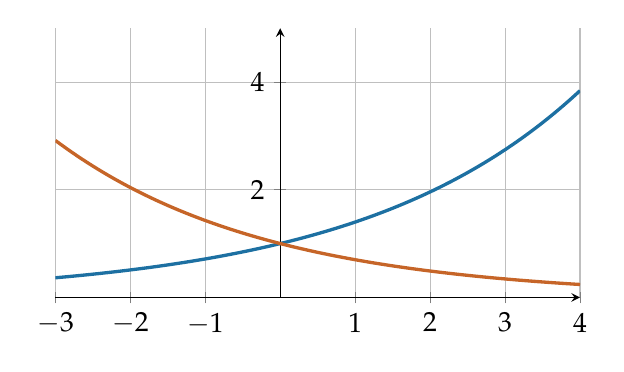
\begin{tikzpicture}\begin{axis}[width=.68\textwidth,height=5cm,axis lines=middle,xmin=-3,xmax=4,ymin=0,ymax=5,grid=major]\addplot[Blue,very thick,samples=100,domain=-3:4]{1.4^x};\addplot[Orange,very thick,samples=100,domain=-3:4]{.7^x};\end{axis}\end{tikzpicture}\end{center}
\end{activite}
\enseignant{$f(t)=12\,000\times1.09^t$, $f(6)\approx20\,126$. The threshold is exceeded from the ninth month onwards. Have students say aloud which piece of data triggers the choice of method.}

\begin{traceecrite}A constant relative change with multiplier $q$ is modelled by $f(t)=V_0q^t$. $V_0$ is the initial value and $q$ the multiplier per unit of time.\end{traceecrite}

\begin{exemple}
Take the data from the investigation and write up the solution in this order: definition of the objects, property used, exact or approximate calculation, then a sentence giving the answer. The model answer appears in the teacher edition.
\end{exemple}
\enseignant{$f(t)=12\,000\times1.09^t$, $f(6)\approx20\,126$. The threshold is exceeded from the ninth month onwards.}

\begin{exercice}[-- essential]
\begin{enumerate}\item Simplify $3^{x+5}\div3^x$ and $(2^x)^3$.\item Study the direction of variation of $f(x)=5\times1.05^x$ and $g(x)=-5\times0.8^x$.\item An initial value of $1650$ increases by $5\,\%$ per year. Give the model and calculate the value after $6$ years.\end{enumerate}
\end{exercice}
\enseignant{$3^5$ et $2^{3x}$. $f$ is increasing; $0.8^x$ is decreasing and the negative coefficient makes $g$ increasing. The model is $V(t)=1650\times\left(1+\dfrac{5}{100}\right)^t$.}

\manuelref{Calao, p. 50, no.~20--25, then p. 53, no.~41}
\ExoSession{13}

\begin{dm}Redo practice exercise 2 with the following data: replace the initial value by $185$ and the rate or common difference/ratio by $3$. Write it up in four lines: data, formula, calculation, conclusion.\end{dm}
\enseignant{The correction depends on the exercise redone. Check above all the consistency of the model, the number of iterations, the rounding and the concluding sentence.}

\begin{sortie}On a half-sheet: write the main rule of the session, work through a very short example and give your confidence level from 1 to 4. Key question(s) of the day: 1, 2 and 3.\end{sortie}

\ifprof
\begin{methode}
\textbf{Running a 1-hour session:} 7 min of fluency; 10 min of sharing and written record; 28 min of essential exercises; 5 min of correction; 3 min of exit ticket.\\
\textbf{Running a 2-hour session:} add 20 min of investigation, 20 min of formalising the rule, a second independent exercise and 10 min of comparative correction.\\
\textbf{Differentiation:} give struggling students a four-box sheet (data, model, calculation, conclusion). Ask fast finishers to produce a counterexample, a justification or a second method.
\end{methode}
\fi
\sessionheader{14}{12 Nov 2026}{B: 1 h -- C: 2 h}{Review and chapter assessment}{Exponential Functions}
\begin{objectifs}\begin{itemize}\item Use what the chapter has covered.\item Write up a modelling solution.\item Correct a mistake.\end{itemize}\end{objectifs}
\begin{automatismes}\begin{enumerate}\item Simplify $3x+3-x+2$. \rep{$2x+5$}\item Is the function $x\mapsto0.7^x$ increasing?? \rep{No, it is decreasing.}\item Compare $1.04^3$ and $1.04^7$. \rep{$1.04^3<1.04^7$}\item Calculer $2^4\times2^3$. \rep{$2^7$}\item Write $5^{-2}$ as a fraction. \rep{$\dfrac1{25}$}\end{enumerate}\end{automatismes}
\begin{prerequis}Reread the last written record and be able to carry out the basic calculations needed today. Before the investigation, have the key words rephrased: use what the chapter has covered and write up a modelling solution.\end{prerequis}

\begin{activite}
Using four pieces of student work, spot and correct: rate/multiplier confusion, a false power rule, an error in the direction of variation and a conclusion without a unit.

\end{activite}
\enseignant{The correction must name the mistake, state the correct rule, redo the calculation and conclude in context. Have students say aloud which piece of data triggers the choice of method.}

\begin{traceecrite}To validate an exponential model: identify $V_0$ and $q$, calculate with the units, check the order of magnitude and interpret the result.\end{traceecrite}

\begin{exemple}
Take the data from the investigation and write up the solution in this order: definition of the objects, property used, exact or approximate calculation, then a sentence giving the answer. The model answer appears in the teacher edition.
\end{exemple}
\enseignant{The correction must name the mistake, state the correct rule, redo the calculation and conclude in context.}

\begin{exercice}[-- essential]
\begin{enumerate}\item Simplify $3^{x+6}\div3^x$ and $(2^x)^3$.\item Study the direction of variation of $f(x)=6\times1.06^x$ and $g(x)=-6\times0.8^x$.\item An initial value of $1700$ increases by $6\,\%$ per year. Give the model and calculate the value after $6$ years.\end{enumerate}
\end{exercice}
\enseignant{$3^6$ et $2^{3x}$. $f$ is increasing; $0.8^x$ is decreasing and the negative coefficient makes $g$ increasing. The model is $V(t)=1700\times\left(1+\dfrac{6}{100}\right)^t$.}

\manuelref{Calao, p. 54, no.~47--58}
\ExoSession{14}

\begin{dm}Redo practice exercise 3 with the following data: replace the initial value by $190$ and the rate or common difference/ratio by $4$. Write it up in four lines: data, formula, calculation, conclusion.\end{dm}
\enseignant{The correction depends on the exercise redone. Check above all the consistency of the model, the number of iterations, the rounding and the concluding sentence.}

\begin{sortie}On a half-sheet: write the main rule of the session, work through a very short example and give your confidence level from 1 to 4. Key question(s) of the day: 1 and 2.\end{sortie}

\ifprof
\begin{methode}
\textbf{Running a 1-hour session:} 7 min of fluency; 10 min of sharing and written record; 28 min of essential exercises; 5 min of correction; 3 min of exit ticket.\\
\textbf{Running a 2-hour session:} add 20 min of investigation, 20 min of formalising the rule, a second independent exercise and 10 min of comparative correction.\\
\textbf{Differentiation:} give struggling students a four-box sheet (data, model, calculation, conclusion). Ask fast finishers to produce a counterexample, a justification or a second method.
\end{methode}
\fi


\chapter{Common logarithm function}
\competences{converting between exponential and logarithmic form, solving, modelling}
\section{Reference notes}
\begin{retenir}
For every $b>0$, $\log(b)$ is the unique real number $x$ such that $10^x=b$. Hence $\log(10^x)=x$ and, for $b>0$, $10^{\log(b)}=b$. The function $\log$ is defined on $]0,+\infty[$ and it is strictly increasing.
\end{retenir}

\begin{center}
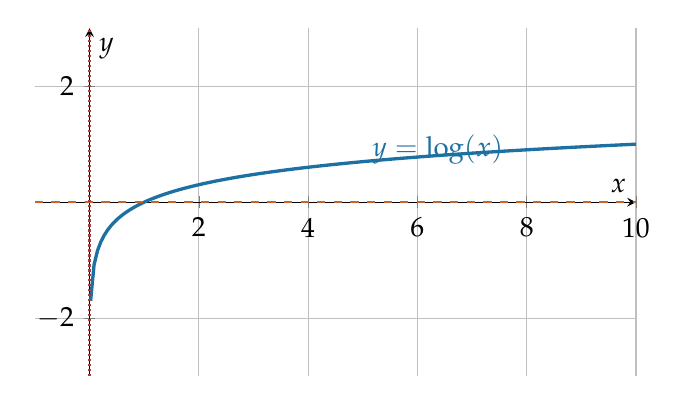
\begin{tikzpicture}
\begin{axis}[width=.76\textwidth,height=6cm,axis lines=middle,xmin=-1,xmax=10,ymin=-3,ymax=3,grid=major,xlabel={$x$},ylabel={$y$}]
\addplot[Blue,very thick,samples=160,domain=.02:10]{ln(x)/ln(10)};
\addplot[Orange,dashed,thick,domain=-1:10]{0};
\addplot[Red,densely dotted,thick] coordinates {(0,-3)(0,3)};
\node[anchor=west,Blue] at (axis cs:5,.9) {$y=\log(x)$};
\end{axis}
\end{tikzpicture}
\end{center}

For $a>0$, $b>0$ and every natural number $n$:
\[
\log(ab)=\log(a)+\log(b),\qquad
\log\!\left(\frac{a}{b}\right)=\log(a)-\log(b),\qquad
\log(a^n)=n\log(a).
\]

\begin{erreur}
$\log(a+b)$ does not simplify. Before any logarithmic calculation, check that each argument is strictly positive.
\end{erreur}

\begin{methode}
To solve $a^x=b$, with $a>0$, $a\neq1$ and $b>0$, take the logarithm: $x\log(a)=\log(b)$, so $x=\dfrac{\log(b)}{\log(a)}$.
\end{methode}

\begin{exemple}
Solving $1.08^x=2$ amounts to writing $x=\dfrac{\log(2)}{\log(1.08)}\approx9.01$. A value multiplied by $1.08$ each year therefore doubles after a little more than nine years.
\end{exemple}

Since $\log$ is increasing, for $a,b>0$, $a<b$ is equivalent to $\log(a)<\log(b)$. For $a>1$, $a^x<b$ is equivalent to $x<\dfrac{\log b}{\log a}$; when $0<a<1$, the inequality sign reverses.

\sessionheader{15}{17 Nov 2026}{B: 2 h -- C: 1 h}{Definition of the common logarithm}{Common logarithm function}
\begin{objectifs}\begin{itemize}\item Link powers of 10 and logarithms.\item Calculate common values.\item Use the calculator.\end{itemize}\end{objectifs}
\begin{automatismes}\begin{enumerate}\item Calculate $20\,\%$ of $80$. \rep{$16$}\item Give the domain of $\log$. \rep{$]0,+\infty[$}\item Calculate $\log(10^4)$. \rep{$4$}\item Solve $10^x=0.01$. \rep{$x=-2$}\item Expand $\log(3b)$, $b>0$. \rep{$\log3+\log b$}\end{enumerate}\end{automatismes}
\begin{prerequis}Reread the last written record and be able to carry out the basic calculations needed today. Before the investigation, have students rephrase the key words: link powers of 10 and logarithms and calculate common values.\end{prerequis}

\begin{activite}
Complete the pairs $10^x=b$ and $x=\log(b)$ for $b=0.001;0.1;1;10;1\,000$. Then use the calculator for $b=7$.

\end{activite}
\enseignant{The logarithms are $-3,-1,0,1,3$; $\log(7)\approx0.8451$. Have students say aloud which piece of data triggers the choice of method.}

\begin{traceecrite}For $b>0$, $\log(b)$ is the unique solution of $10^x=b$. In particular $\log(1)=0$, $\log(10)=1$ and $\log(100)=2$.\end{traceecrite}

\begin{exemple}
Revisit the data from the investigation and write up the solution in order: definition of the objects, property used, exact or approximate calculation, then a concluding sentence. The model answer appears in the teacher edition.
\end{exemple}
\enseignant{The logarithms are $-3,-1,0,1,3$; $\log(7)\approx0.8451$.}

\begin{exercice}[-- essential]
\begin{enumerate}\item Calculate $\log(10^2)$ and $\log(10^{-2})$.\item Expand $\log\!\left(\dfrac{100a^2}{b}\right)$ for $a,b>0$.\item Solve $2^x=22$ and give an approximate value to the nearest hundredth.\end{enumerate}
\end{exercice}
\enseignant{$2$ and $-2$. The expression equals $2+2\log(a)-\log(b)$. Finally $x=\dfrac{\log(22)}{\log(2)}$.}

\manuelref{Calao, course pp. 64--69; exercises p. 70, no.~1--5}
\CalaoSession{15}

\begin{dm}Redo practice exercise 2 with the following data: replace the initial value by $195$ and the rate or common ratio by $5$. Write it up in four lines: data, formula, calculation, conclusion.\end{dm}
\enseignant{The answer depends on the exercise revisited. Check above all the consistency of the model, the number of iterations, the rounding and the concluding sentence.}

\begin{sortie}On a half-sheet: write the main rule of the session, work through a very short example and state your confidence level from 1 to 4. Key question(s) of the day: 1, 2 and 3.\end{sortie}

\ifprof
\begin{methode}
\textbf{1 h session:} 7 min of fluency; 10 min of pooling and written record; 28 min of essential exercises; 5 min of correction; 3 min of exit ticket.\\
\textbf{2 h session:} add 20 min of investigation, 20 min of formalisation, a second independent exercise and 10 min of comparative correction.\\
\textbf{Differentiation:} give struggling students a four-box sheet (data, model, calculation, conclusion). Ask quick students to produce a counterexample, a justification or a second method.
\end{methode}
\fi
\sessionheader{16}{19 Nov 2026}{B: 1 h -- C: 2 h}{Variations and graph}{Common logarithm function}
\begin{objectifs}\begin{itemize}\item Know the domain.\item Use the fact that the function is increasing.\item Read the curve.\end{itemize}\end{objectifs}
\begin{automatismes}\begin{enumerate}\item Write the multiplier for an increase of $25\,\%$. \rep{$1+\dfrac{25}{100}=1.25$}\item Calculate $\log(10^0)$. \rep{$0$}\item Solve $10^x=0.01$. \rep{$x=-2$}\item Expand $\log(3b)$, $b>0$. \rep{$\log3+\log b$}\item Give the domain of $\log$. \rep{$]0,+\infty[$}\end{enumerate}\end{automatismes}
\begin{prerequis}Reread the last written record and be able to carry out the basic calculations needed today. Before the investigation, have students rephrase the key words: know the domain and use the fact that the function is increasing.\end{prerequis}

\begin{activite}
Plot $y=10^x$ and the line $y=x$, then obtain the curve of the logarithm by symmetry. Deduce its domain, its direction of variation and its asymptote.
\begin{center}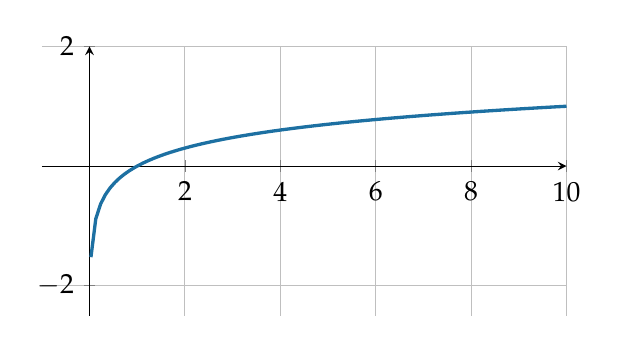
\begin{tikzpicture}\begin{axis}[width=.68\textwidth,height=5cm,axis lines=middle,xmin=-1,xmax=10,ymin=-2.5,ymax=2,grid=major]\addplot[Blue,very thick,samples=100,domain=.03:10]{ln(x)/ln(10)};\end{axis}\end{tikzpicture}\end{center}
\end{activite}
\enseignant{The logarithm is the inverse function of $10^x$: domain $]0,+\infty[$, strictly increasing, asymptote $x=0$. Have students say aloud which piece of data triggers the choice of method.}

\begin{traceecrite}The function $\log$ is defined on $]0,+\infty[$, is strictly increasing, and its curve has $x=0$ as a vertical asymptote.\end{traceecrite}

\begin{exemple}
Revisit the data from the investigation and write up the solution in order: definition of the objects, property used, exact or approximate calculation, then a concluding sentence. The model answer appears in the teacher edition.
\end{exemple}
\enseignant{The logarithm is the inverse function of $10^x$: domain $]0,+\infty[$, strictly increasing, asymptote $x=0$.}

\begin{exercice}[-- essential]
\begin{enumerate}\item Calculate $\log(10^3)$ and $\log(10^{-3})$.\item Expand $\log\!\left(\dfrac{100a^2}{b}\right)$ for $a,b>0$.\item Solve $3^x=23$ and give an approximate value to the nearest hundredth.\end{enumerate}
\end{exercice}
\enseignant{$3$ and $-3$. The expression equals $2+2\log(a)-\log(b)$. Finally $x=\dfrac{\log(23)}{\log(3)}$.}

\manuelref{Calao, course pp. 64--69; exercises p. 70, no.~6--10}
\CalaoSession{16}

\begin{dm}Redo practice exercise 3 with the following data: replace the initial value by $200$ and the rate or common ratio by $6$. Write it up in four lines: data, formula, calculation, conclusion.\end{dm}
\enseignant{The answer depends on the exercise revisited. Check above all the consistency of the model, the number of iterations, the rounding and the concluding sentence.}

\begin{sortie}On a half-sheet: write the main rule of the session, work through a very short example and state your confidence level from 1 to 4. Key question(s) of the day: 1 and 2.\end{sortie}

\ifprof
\begin{methode}
\textbf{1 h session:} 7 min of fluency; 10 min of pooling and written record; 28 min of essential exercises; 5 min of correction; 3 min of exit ticket.\\
\textbf{2 h session:} add 20 min of investigation, 20 min of formalisation, a second independent exercise and 10 min of comparative correction.\\
\textbf{Differentiation:} give struggling students a four-box sheet (data, model, calculation, conclusion). Ask quick students to produce a counterexample, a justification or a second method.
\end{methode}
\fi
\sessionheader{17}{24 Nov 2026}{B: 2 h -- C: 1 h}{Algebraic properties}{Common logarithm function}
\begin{objectifs}\begin{itemize}\item Expand or condense logarithms.\item Check the conditions.\item Avoid false properties.\end{itemize}\end{objectifs}
\begin{automatismes}\begin{enumerate}\item Simplify $3x+6-x+2$. \rep{$2x+8$}\item Solve $10^x=0.01$. \rep{$x=-2$}\item Expand $\log(3b)$, $b>0$. \rep{$\log3+\log b$}\item Give the domain of $\log$. \rep{$]0,+\infty[$}\item Calculate $\log(10^1)$. \rep{$1$}\end{enumerate}\end{automatismes}
\begin{prerequis}Reread the last written record and be able to carry out the basic calculations needed today. Before the investigation, have students rephrase the key words: expand or condense logarithms and check the conditions.\end{prerequis}

\begin{activite}
Starting from $10^2\times10^3=10^5$, conjecture $\log(ab)=\log a+\log b$. Test numerically with $a=2,b=5$, then explain why $a,b$ must be positive.

\end{activite}
\enseignant{$\log(2)+\log(5)=\log(10)=1$. The logarithm is only defined for a strictly positive argument. Have students say aloud which piece of data triggers the choice of method.}

\begin{traceecrite}For $a,b>0$, $\log(ab)=\log a+\log b$ and $\log\!\left(\dfrac ab\right)=\log a-\log b$. Moreover $\log(a^n)=n\log a$.\end{traceecrite}

\begin{exemple}
Revisit the data from the investigation and write up the solution in order: definition of the objects, property used, exact or approximate calculation, then a concluding sentence. The model answer appears in the teacher edition.
\end{exemple}
\enseignant{$\log(2)+\log(5)=\log(10)=1$. The logarithm is only defined for a strictly positive argument.}

\begin{exercice}[-- essential]
\begin{enumerate}\item Calculate $\log(10^4)$ and $\log(10^{-4})$.\item Expand $\log\!\left(\dfrac{100a^2}{b}\right)$ for $a,b>0$.\item Solve $4^x=24$ and give an approximate value to the nearest hundredth.\end{enumerate}
\end{exercice}
\enseignant{$4$ and $-4$. The expression equals $2+2\log(a)-\log(b)$. Finally $x=\dfrac{\log(24)}{\log(4)}$.}

\manuelref{Calao, course pp. 66--69; exercises p. 72, no.~20--23}
\CalaoSession{17}

\begin{dm}Redo practice exercise 2 with the following data: replace the initial value by $205$ and the rate or common ratio by $7$. Write it up in four lines: data, formula, calculation, conclusion.\end{dm}
\enseignant{The answer depends on the exercise revisited. Check above all the consistency of the model, the number of iterations, the rounding and the concluding sentence.}

\begin{sortie}On a half-sheet: write the main rule of the session, work through a very short example and state your confidence level from 1 to 4. Key question(s) of the day: 1, 2 and 3.\end{sortie}

\ifprof
\begin{methode}
\textbf{1 h session:} 7 min of fluency; 10 min of pooling and written record; 28 min of essential exercises; 5 min of correction; 3 min of exit ticket.\\
\textbf{2 h session:} add 20 min of investigation, 20 min of formalisation, a second independent exercise and 10 min of comparative correction.\\
\textbf{Differentiation:} give struggling students a four-box sheet (data, model, calculation, conclusion). Ask quick students to produce a counterexample, a justification or a second method.
\end{methode}
\fi
\sessionheader{18}{26 Nov 2026}{B: 1 h -- C: 2 h}{Solving $10^x=b$}{Common logarithm function}
\begin{objectifs}\begin{itemize}\item Solve $10^x=b$.\item Bracket a solution.\item Interpret an order of magnitude.\end{itemize}\end{objectifs}
\begin{automatismes}\begin{enumerate}\item Calculate $5\,\%$ of $140$. \rep{$7$}\item Expand $\log(3b)$, $b>0$. \rep{$\log3+\log b$}\item Give the domain of $\log$. \rep{$]0,+\infty[$}\item Calculate $\log(10^2)$. \rep{$2$}\item Solve $10^x=0.01$. \rep{$x=-2$}\end{enumerate}\end{automatismes}
\begin{prerequis}Reread the last written record and be able to carry out the basic calculations needed today. Before the investigation, have students rephrase the key words: solve $10^x=b$ and bracket a solution.\end{prerequis}

\begin{activite}
A device measures intensities $b=0.04;3.2;850$. For each value, solve $10^x=b$, give $x$ to the nearest hundredth and check by calculating $10^x$.

\end{activite}
\enseignant{$x=\log(b)$: approximately $-1.40$, $0.51$ and $2.93$. Have students say aloud which piece of data triggers the choice of method.}

\begin{traceecrite}The equation $10^x=b$ has a solution only if $b>0$; this solution is $x=\log(b)$.\end{traceecrite}

\begin{exemple}
Revisit the data from the investigation and write up the solution in order: definition of the objects, property used, exact or approximate calculation, then a concluding sentence. The model answer appears in the teacher edition.
\end{exemple}
\enseignant{$x=\log(b)$: approximately $-1.40$, $0.51$ and $2.93$.}

\begin{exercice}[-- essential]
\begin{enumerate}\item Calculate $\log(10^5)$ and $\log(10^{-5})$.\item Expand $\log\!\left(\dfrac{100a^2}{b}\right)$ for $a,b>0$.\item Solve $5^x=25$ and give an approximate value to the nearest hundredth.\end{enumerate}
\end{exercice}
\enseignant{$5$ and $-5$. The expression equals $2+2\log(a)-\log(b)$. Finally $x=\dfrac{\log(25)}{\log(5)}$.}

\manuelref{Calao, p. 73, no.~30--32}
\CalaoSession{18}

\begin{dm}Redo practice exercise 3 with the following data: replace the initial value by $210$ and the rate or common ratio by $2$. Write it up in four lines: data, formula, calculation, conclusion.\end{dm}
\enseignant{The answer depends on the exercise revisited. Check above all the consistency of the model, the number of iterations, the rounding and the concluding sentence.}

\begin{sortie}On a half-sheet: write the main rule of the session, work through a very short example and state your confidence level from 1 to 4. Key question(s) of the day: 1 and 2.\end{sortie}

\ifprof\clearpage
\begin{methode}
\textbf{1 h session:} 7 min of fluency; 10 min of pooling and written record; 28 min of essential exercises; 5 min of correction; 3 min of exit ticket.\\
\textbf{2 h session:} add 20 min of investigation, 20 min of formalisation, a second independent exercise and 10 min of comparative correction.\\
\textbf{Differentiation:} give struggling students a four-box sheet (data, model, calculation, conclusion). Ask quick students to produce a counterexample, a justification or a second method.
\end{methode}
\fi
\sessionheader{19}{1 Dec 2026}{B: 2 h -- C: 1 h}{Solving $a^x=b$}{Common logarithm function}
\begin{objectifs}\begin{itemize}\item Solve $a^x=b$.\item Use a quotient of logarithms.\item Round sensibly.\end{itemize}\end{objectifs}
\begin{automatismes}\begin{enumerate}\item Write the multiplier for an increase of $10\,\%$. \rep{$1+\dfrac{10}{100}=1.10$}\item Give the domain of $\log$. \rep{$]0,+\infty[$}\item Calculate $\log(10^3)$. \rep{$3$}\item Solve $10^x=0.01$. \rep{$x=-2$}\item Expand $\log(3b)$, $b>0$. \rep{$\log3+\log b$}\end{enumerate}\end{automatismes}
\begin{prerequis}Reread the last written record and be able to carry out the basic calculations needed today. Before the investigation, have students rephrase the key words: solve $a^x=b$ and use a quotient of logarithms.\end{prerequis}

\begin{activite}
The number of subscribers is multiplied by $1.15$ each month. Determine after how many months it will have tripled. Set up the equation, solve it using logarithms and interpret the rounding.

\end{activite}
\enseignant{$1.15^n\geq3$; $\dfrac{\log3}{\log1.15}\approx7.86$. So eight whole months are needed. Have students say aloud which piece of data triggers the choice of method.}

\begin{traceecrite}For $a>0$, $a\neq1$ and $b>0$, $a^x=b$ is equivalent to $x=\dfrac{\log(b)}{\log(a)}$.\end{traceecrite}

\begin{exemple}
Revisit the data from the investigation and write up the solution in order: definition of the objects, property used, exact or approximate calculation, then a concluding sentence. The model answer appears in the teacher edition.
\end{exemple}
\enseignant{$1.15^n\geq3$; $\dfrac{\log3}{\log1.15}\approx7.86$. So eight whole months are needed.}

\begin{exercice}[-- essential]
\begin{enumerate}\item Calculate $\log(10^6)$ and $\log(10^{-6})$.\item Expand $\log\!\left(\dfrac{100a^2}{b}\right)$ for $a,b>0$.\item Solve $6^x=26$ and give an approximate value to the nearest hundredth.\end{enumerate}
\end{exercice}
\enseignant{$6$ and $-6$. The expression equals $2+2\log(a)-\log(b)$. Finally $x=\dfrac{\log(26)}{\log(6)}$.}

\manuelref{Calao, p. 74, no.~33--39}
\CalaoSession{19}

\begin{dm}Redo practice exercise 2 with the following data: replace the initial value by $215$ and the rate or common ratio by $3$. Write it up in four lines: data, formula, calculation, conclusion.\end{dm}
\enseignant{The answer depends on the exercise revisited. Check above all the consistency of the model, the number of iterations, the rounding and the concluding sentence.}

\begin{sortie}On a half-sheet: write the main rule of the session, work through a very short example and state your confidence level from 1 to 4. Key question(s) of the day: 1, 2 and 3.\end{sortie}

\ifprof
\begin{methode}
\textbf{1 h session:} 7 min of fluency; 10 min of pooling and written record; 28 min of essential exercises; 5 min of correction; 3 min of exit ticket.\\
\textbf{2 h session:} add 20 min of investigation, 20 min of formalisation, a second independent exercise and 10 min of comparative correction.\\
\textbf{Differentiation:} give struggling students a four-box sheet (data, model, calculation, conclusion). Ask quick students to produce a counterexample, a justification or a second method.
\end{methode}
\fi
\sessionheader{20}{3 Dec 2026}{B: 1 h -- C: 2 h}{Equations $x^a=b$ and simple inequalities}{Common logarithm function}
\begin{objectifs}\begin{itemize}\item Solve equations where the variable is the base.\item Deal with an inequality.\item Take the domain into account.\end{itemize}\end{objectifs}
\begin{automatismes}\begin{enumerate}\item Simplify $3x+9-x+2$. \rep{$2x+11$}\item Calculate $\log(10^4)$. \rep{$4$}\item Solve $10^x=0.01$. \rep{$x=-2$}\item Expand $\log(3b)$, $b>0$. \rep{$\log3+\log b$}\item Give the domain of $\log$. \rep{$]0,+\infty[$}\end{enumerate}\end{automatismes}
\begin{prerequis}Reread the last written record and be able to carry out the basic calculations needed today. Before the investigation, have students rephrase the key words: solve equations where the variable is the base and deal with an inequality.\end{prerequis}

\begin{activite}
Solve on $[0,+\infty[$: $x^3=40$, then $x^4=16$. Then solve $1.08^x<1.5$ and explain the role of the function being increasing.

\end{activite}
\enseignant{$x=\sqrt[3]{40}\approx3.42$; $x=2$ on the requested interval; $x<\dfrac{\log1.5}{\log1.08}\approx5.27$. Have students say aloud which piece of data triggers the choice of method.}

\begin{traceecrite}To solve $x^n=b$, take the domain and the parity of $n$ into account. For an exponential inequality, the direction depends on whether the function is increasing or decreasing.\end{traceecrite}

\begin{exemple}
Revisit the data from the investigation and write up the solution in order: definition of the objects, property used, exact or approximate calculation, then a concluding sentence. The model answer appears in the teacher edition.
\end{exemple}
\enseignant{$x=\sqrt[3]{40}\approx3.42$; $x=2$ on the requested interval; $x<\dfrac{\log1.5}{\log1.08}\approx5.27$.}

\begin{exercice}[-- essential]
\begin{enumerate}\item Calculate $\log(10^2)$ and $\log(10^{-2})$.\item Expand $\log\!\left(\dfrac{100a^2}{b}\right)$ for $a,b>0$.\item Solve $2^x=22$ and give an approximate value to the nearest hundredth.\end{enumerate}
\end{exercice}
\enseignant{$2$ and $-2$. The expression equals $2+2\log(a)-\log(b)$. Finally $x=\dfrac{\log(22)}{\log(2)}$.}

\manuelref{Calao, p. 75, no.~40--42}
\CalaoSession{20}

\begin{dm}Redo practice exercise 3 with the following data: replace the initial value by $220$ and the rate or common ratio by $4$. Write it up in four lines: data, formula, calculation, conclusion.\end{dm}
\enseignant{The answer depends on the exercise revisited. Check above all the consistency of the model, the number of iterations, the rounding and the concluding sentence.}

\begin{sortie}On a half-sheet: write the main rule of the session, work through a very short example and state your confidence level from 1 to 4. Key question(s) of the day: 1 and 2.\end{sortie}

\ifprof\clearpage
\begin{methode}
\textbf{1 h session:} 7 min of fluency; 10 min of pooling and written record; 28 min of essential exercises; 5 min of correction; 3 min of exit ticket.\\
\textbf{2 h session:} add 20 min of investigation, 20 min of formalisation, a second independent exercise and 10 min of comparative correction.\\
\textbf{Differentiation:} give struggling students a four-box sheet (data, model, calculation, conclusion). Ask quick students to produce a counterexample, a justification or a second method.
\end{methode}
\fi
\sessionheader{21}{8 Dec 2026}{B: 2 h -- C: 1 h}{Problems in context}{Common logarithm function}
\begin{objectifs}\begin{itemize}\item Model a situation.\item Choose an equation.\item Conclude in context.\end{itemize}\end{objectifs}
\begin{automatismes}\begin{enumerate}\item Calculate $20\,\%$ of $60$. \rep{$12$}\item Solve $10^x=0.01$. \rep{$x=-2$}\item Expand $\log(3b)$, $b>0$. \rep{$\log3+\log b$}\item Give the domain of $\log$. \rep{$]0,+\infty[$}\item Calculate $\log(10^3)$. \rep{$3$}\end{enumerate}\end{automatismes}
\begin{prerequis}Reread the last written record and be able to carry out the basic calculations needed today. Before the investigation, have students rephrase the key words: model a situation and choose an equation.\end{prerequis}

\begin{activite}
The sound level is $L=10\log\!\left(\dfrac I{I_0}\right)$. Calculate $L$ when $I=10^6I_0$. Then determine the ratio $\dfrac I{I_0}$ for $L=85$ dB.

\end{activite}
\enseignant{$L=60$ dB. For $85$ dB, $\log\!\left(\dfrac I{I_0}\right)=8.5$, so $\dfrac I{I_0}=10^{8.5}\approx3.16\times10^8$. Have students say aloud which piece of data triggers the choice of method.}

\begin{traceecrite}In a problem, define the variable, set up the equation, solve, check the domain and conclude with the unit. A numerical solution without interpretation is incomplete.\end{traceecrite}

\begin{exemple}
Revisit the data from the investigation and write up the solution in order: definition of the objects, property used, exact or approximate calculation, then a concluding sentence. The model answer appears in the teacher edition.
\end{exemple}
\enseignant{$L=60$ dB. For $85$ dB, $\log\!\left(\dfrac I{I_0}\right)=8.5$, so $\dfrac I{I_0}=10^{8.5}\approx3.16\times10^8$.}

\begin{exercice}[-- essential]
\begin{enumerate}\item Calculate $\log(10^3)$ and $\log(10^{-3})$.\item Expand $\log\!\left(\dfrac{100a^2}{b}\right)$ for $a,b>0$.\item Solve $3^x=23$ and give an approximate value to the nearest hundredth.\end{enumerate}
\end{exercice}
\enseignant{$3$ and $-3$. The expression equals $2+2\log(a)-\log(b)$. Finally $x=\dfrac{\log(23)}{\log(3)}$.}

\manuelref{Calao, p. 74, no.~38--39, then p. 75, no.~40--42}
\CalaoSession{21}

\begin{dm}Redo practice exercise 2 with the following data: replace the initial value by $225$ and the rate or common ratio by $5$. Write it up in four lines: data, formula, calculation, conclusion.\end{dm}
\enseignant{The answer depends on the exercise revisited. Check above all the consistency of the model, the number of iterations, the rounding and the concluding sentence.}

\begin{sortie}On a half-sheet: write the main rule of the session, work through a very short example and state your confidence level from 1 to 4. Key question(s) of the day: 1, 2 and 3.\end{sortie}

\ifprof
\begin{methode}
\textbf{1 h session:} 7 min of fluency; 10 min of pooling and written record; 28 min of essential exercises; 5 min of correction; 3 min of exit ticket.\\
\textbf{2 h session:} add 20 min of investigation, 20 min of formalisation, a second independent exercise and 10 min of comparative correction.\\
\textbf{Differentiation:} give struggling students a four-box sheet (data, model, calculation, conclusion). Ask quick students to produce a counterexample, a justification or a second method.
\end{methode}
\fi
\sessionheader{22}{10 Dec 2026}{B: 1 h -- C: 2 h}{Review and assessment}{Common logarithm function}
\begin{objectifs}\begin{itemize}\item Summarise the methods.\item Identify the conditions.\item Correct mistakes.\end{itemize}\end{objectifs}
\begin{automatismes}\begin{enumerate}\item Write the multiplier for an increase of $25\,\%$. \rep{$1+\dfrac{25}{100}=1.25$}\item Expand $\log(3b)$, $b>0$. \rep{$\log3+\log b$}\item Give the domain of $\log$. \rep{$]0,+\infty[$}\item Calculate $\log(10^4)$. \rep{$4$}\item Solve $10^x=0.01$. \rep{$x=-2$}\end{enumerate}\end{automatismes}
\begin{prerequis}Reread the last written record and be able to carry out the basic calculations needed today. Before the investigation, have students rephrase the key words: summarise the methods and identify the conditions.\end{prerequis}

\begin{activite}
Make a map of methods: domain; properties; equations $10^x=b$; equations $a^x=b$; inequalities. Attach a condition and an example to each branch.

\end{activite}
\enseignant{The map should in particular show that arguments must be positive and the distinction between a base greater than $1$ and one between $0$ and $1$. Have students say aloud which piece of data triggers the choice of method.}

\begin{traceecrite}Before calculating a logarithm: check positivity. Before a comparison: identify the direction of variation. Before a conclusion: check that the result is plausible.\end{traceecrite}

\begin{exemple}
Revisit the data from the investigation and write up the solution in order: definition of the objects, property used, exact or approximate calculation, then a concluding sentence. The model answer appears in the teacher edition.
\end{exemple}
\enseignant{The map should in particular show that arguments must be positive and the distinction between a base greater than $1$ and one between $0$ and $1$.}

\begin{exercice}[-- essential]
\begin{enumerate}\item Calculate $\log(10^4)$ and $\log(10^{-4})$.\item Expand $\log\!\left(\dfrac{100a^2}{b}\right)$ for $a,b>0$.\item Solve $4^x=24$ and give an approximate value to the nearest hundredth.\end{enumerate}
\end{exercice}
\enseignant{$4$ and $-4$. The expression equals $2+2\log(a)-\log(b)$. Finally $x=\dfrac{\log(24)}{\log(4)}$.}

\manuelref{Calao, pp. 76--79}
\CalaoSession{22}

\begin{dm}Redo practice exercise 3 with the following data: replace the initial value by $230$ and the rate or common ratio by $6$. Write it up in four lines: data, formula, calculation, conclusion.\end{dm}
\enseignant{The answer depends on the exercise revisited. Check above all the consistency of the model, the number of iterations, the rounding and the concluding sentence.}

\begin{sortie}On a half-sheet: write the main rule of the session, work through a very short example and state your confidence level from 1 to 4. Key question(s) of the day: 1 and 2.\end{sortie}

\ifprof
\begin{methode}
\textbf{1 h session:} 7 min of fluency; 10 min of pooling and written record; 28 min of essential exercises; 5 min of correction; 3 min of exit ticket.\\
\textbf{2 h session:} add 20 min of investigation, 20 min of formalisation, a second independent exercise and 10 min of comparative correction.\\
\textbf{Differentiation:} give struggling students a four-box sheet (data, model, calculation, conclusion). Ask quick students to produce a counterexample, a justification or a second method.
\end{methode}
\fi


\chapter{Reciprocal (inverse) function}
\competences{finding a domain, differentiating, studying a sign, drawing up a table of variations, graphing}
\section{Reference notes}
The reciprocal function is defined by $f(x)=\dfrac1x$ on $\R\setminus\{0\}$.

\begin{center}
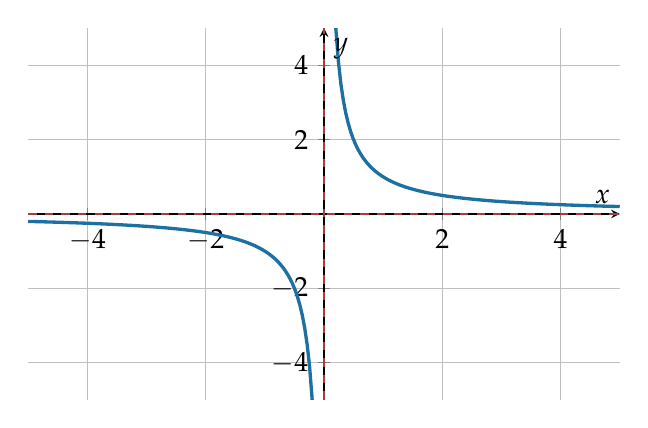
\begin{tikzpicture}
\begin{axis}[width=.75\textwidth,height=6.3cm,axis lines=middle,xmin=-5,xmax=5,ymin=-5,ymax=5,grid=major,xlabel={$x$},ylabel={$y$},unbounded coords=jump]
\addplot[Blue,very thick,samples=120,domain=-5:-.12]{1/x};
\addplot[Blue,very thick,samples=120,domain=.12:5]{1/x};
\addplot[Red,dashed,thick] coordinates {(0,-5)(0,5)};
\addplot[Red,dashed,thick] coordinates {(-5,0)(5,0)};
\end{axis}
\end{tikzpicture}
\end{center}

\begin{retenir}
$f'(x)=-\dfrac1{x^2}<0$ for every $x\neq0$. The reciprocal function is strictly decreasing on each of the intervals $]-\infty,0[$ and $]0,+\infty[$. The lines $x=0$ and $y=0$ are asymptotes.
\end{retenir}

\begin{erreur}
One cannot write that the reciprocal function is decreasing ``on $\R\setminus\{0\}$'' without specifying the two intervals. For example $-1<1$ but $f(-1)=-1<1=f(1)$, which would contradict the global definition of decreasing.
\end{erreur}

For a function $g(x)=P(x)+\dfrac{k}{x}$, proceed in this order: domain; derivative; common denominator and factorisation; sign of the derivative; variations; limits or behaviour at the boundaries; useful points; graph.

\begin{exemple}
On $]0,+\infty[$, $g(x)=x+\dfrac4x$ satisfies $g'(x)=1-\dfrac4{x^2}=\dfrac{(x-2)(x+2)}{x^2}$. The denominator is positive; $g'$ is negative on $]0,2[$ then positive on $]2,+\infty[$. The function has a minimum $g(2)=4$.
\end{exemple}

\sessionheader{23}{15 Dec 2026}{B: 2 h -- C: 1 h}{Definition and graph of the reciprocal function}{Reciprocal (inverse) function}
\begin{objectifs}\begin{itemize}\item Find the domain.\item Draw the curve.\item Use symmetries.\end{itemize}\end{objectifs}
\begin{automatismes}\begin{enumerate}\item Simplify $3x+5-x+2$. \rep{$2x+7$}\item Give the excluded value of $\dfrac{x+1}{x}$. \rep{$x=0$}\item Calculate $\dfrac1{5}$ and $\dfrac1{-5}$. \rep{$\dfrac1{5}$ and $-\dfrac1{5}$}\item Differentiate $3x^2-5x+1$. \rep{$6x-5$}\item Solve $(x-2)(x+1)=0$. \rep{$x=-1$ or $x=2$}\end{enumerate}\end{automatismes}
\begin{prerequis}Reread the last written record and be able to carry out the basic calculations needed today. Before the investigation, have students rephrase the key words: find the domain and draw the curve.\end{prerequis}

\begin{activite}
Calculate $\dfrac1x$ for $x=-4,-2,-1,-\dfrac12,\dfrac12,1,2,4$. Plot the points and describe the symmetries. Why is $x=0$ missing?
\begin{center}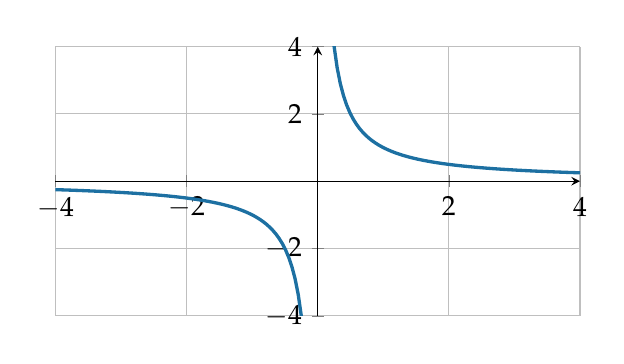
\begin{tikzpicture}\begin{axis}[width=.68\textwidth,height=5cm,axis lines=middle,xmin=-4,xmax=4,ymin=-4,ymax=4,grid=major]\addplot[Blue,very thick,samples=80,domain=-4:-.15]{1/x};\addplot[Blue,very thick,samples=80,domain=.15:4]{1/x};\end{axis}\end{tikzpicture}\end{center}
\end{activite}
\enseignant{The values are respectively $-\frac14,-\frac12,-1,-2,2,1,\frac12,\frac14$. The domain excludes $0$; the curve is symmetric about the origin. Have students say aloud which piece of data triggers the choice of method.}

\begin{traceecrite}The reciprocal function is $f(x)=\dfrac1x$ on $\R\setminus\{0\}$. Its curve is a hyperbola symmetric about the origin.\end{traceecrite}

\begin{exemple}
Revisit the data from the investigation and write up the solution in order: definition of the objects, property used, exact or approximate calculation, then a concluding sentence. The model answer appears in the teacher edition.
\end{exemple}
\enseignant{The values are respectively $-\frac14,-\frac12,-1,-2,2,1,\frac12,\frac14$. The domain excludes $0$; the curve is symmetric about the origin.}

\begin{exercice}[-- essential]
\begin{enumerate}\item Give the domain and the asymptotes of $f(x)=5+\dfrac{7}x$.\item Calculate $f'(x)$ and study its sign.\item Study the function $g(x)=x+\dfrac{25}x$ on $]0,+\infty[$.\end{enumerate}
\end{exercice}
\enseignant{The domain is $\R\setminus\{0\}$; asymptotes $x=0$ and $y=5$. $f'(x)=-\dfrac{7}{x^2}<0$. For $g$, $g'(x)=1-\dfrac{25}{x^2}$ and the minimum is reached at $x=5$, with value $10$.}

\manuelref{Calao, course pp. 88--93; exercises p. 94, no.~1--5}
\CalaoSession{23}

\begin{dm}Redo practice exercise 2 with the following data: replace the initial value by $235$ and the rate or common ratio by $7$. Write it up in four lines: data, formula, calculation, conclusion.\end{dm}
\enseignant{The answer depends on the exercise revisited. Check above all the consistency of the model, the number of iterations, the rounding and the concluding sentence.}

\begin{sortie}On a half-sheet: write the main rule of the session, work through a very short example and state your confidence level from 1 to 4. Key question(s) of the day: 1, 2 and 3.\end{sortie}

\ifprof
\begin{methode}
\textbf{1 h session:} 7 min of fluency; 10 min of pooling and written record; 28 min of essential exercises; 5 min of correction; 3 min of exit ticket.\\
\textbf{2 h session:} add 20 min of investigation, 20 min of formalisation, a second independent exercise and 10 min of comparative correction.\\
\textbf{Differentiation:} give struggling students a four-box sheet (data, model, calculation, conclusion). Ask quick students to produce a counterexample, a justification or a second method.
\end{methode}
\fi
\sessionheader{24}{17 Dec 2026}{B: 1 h -- C: 2 h}{Behaviour at the boundaries and asymptotes}{Reciprocal (inverse) function}
\begin{objectifs}\begin{itemize}\item Describe the behaviour at the boundaries.\item Identify the asymptotes.\item Read a graph.\end{itemize}\end{objectifs}
\begin{automatismes}\begin{enumerate}\item Calculate $5\,\%$ of $120$. \rep{$6$}\item Calculate $\dfrac1{6}$ and $\dfrac1{-6}$. \rep{$\dfrac1{6}$ and $-\dfrac1{6}$}\item Differentiate $3x^2-5x+1$. \rep{$6x-5$}\item Solve $(x-2)(x+1)=0$. \rep{$x=-1$ or $x=2$}\item Give the excluded value of $\dfrac{x+1}{x}$. \rep{$x=0$}\end{enumerate}\end{automatismes}
\begin{prerequis}Reread the last written record and be able to carry out the basic calculations needed today. Before the investigation, have students rephrase the key words: describe the behaviour at the boundaries and identify the asymptotes.\end{prerequis}

\begin{activite}
Using a table of values near $0$ and for large values of $|x|$, describe $\dfrac1x$. Translate each behaviour into an asymptote and a sentence.
\begin{center}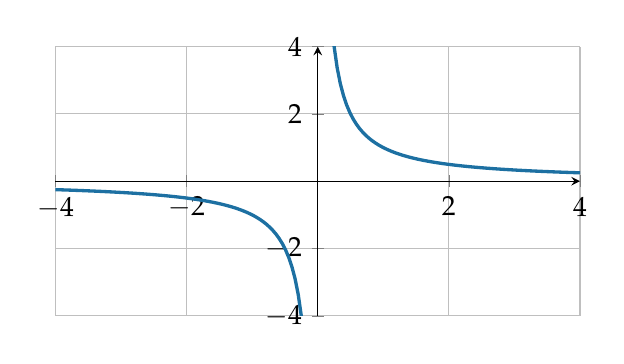
\begin{tikzpicture}\begin{axis}[width=.68\textwidth,height=5cm,axis lines=middle,xmin=-4,xmax=4,ymin=-4,ymax=4,grid=major]\addplot[Blue,very thick,samples=80,domain=-4:-.15]{1/x};\addplot[Blue,very thick,samples=80,domain=.15:4]{1/x};\end{axis}\end{tikzpicture}\end{center}
\end{activite}
\enseignant{Near $0$, the values become very large in absolute value: asymptote $x=0$. As $|x|$ grows, $\dfrac1x$ gets closer to $0$: asymptote $y=0$. Have students say aloud which piece of data triggers the choice of method.}

\begin{traceecrite}For $f(x)=\dfrac1x$, $x=0$ is a vertical asymptote and $y=0$ a horizontal asymptote. The branches approach them without crossing them.\end{traceecrite}

\begin{exemple}
Revisit the data from the investigation and write up the solution in order: definition of the objects, property used, exact or approximate calculation, then a concluding sentence. The model answer appears in the teacher edition.
\end{exemple}
\enseignant{Near $0$, the values become very large in absolute value: asymptote $x=0$. As $|x|$ grows, $\dfrac1x$ gets closer to $0$: asymptote $y=0$.}

\begin{exercice}[-- essential]
\begin{enumerate}\item Give the domain and the asymptotes of $f(x)=6+\dfrac{8}x$.\item Calculate $f'(x)$ and study its sign.\item Study the function $g(x)=x+\dfrac{36}x$ on $]0,+\infty[$.\end{enumerate}
\end{exercice}
\enseignant{The domain is $\R\setminus\{0\}$; asymptotes $x=0$ and $y=6$. $f'(x)=-\dfrac{8}{x^2}<0$. For $g$, $g'(x)=1-\dfrac{36}{x^2}$ and the minimum is reached at $x=6$, with value $12$.}

\manuelref{Calao, course pp. 88--93; exercises p. 94, no.~4--9}
\CalaoSession{24}

\begin{dm}Redo practice exercise 3 with the following data: replace the initial value by $240$ and the rate or common ratio by $2$. Write it up in four lines: data, formula, calculation, conclusion.\end{dm}
\enseignant{The answer depends on the exercise revisited. Check above all the consistency of the model, the number of iterations, the rounding and the concluding sentence.}

\begin{sortie}On a half-sheet: write the main rule of the session, work through a very short example and state your confidence level from 1 to 4. Key question(s) of the day: 1 and 2.\end{sortie}

\ifprof
\begin{methode}
\textbf{1 h session:} 7 min of fluency; 10 min of pooling and written record; 28 min of essential exercises; 5 min of correction; 3 min of exit ticket.\\
\textbf{2 h session:} add 20 min of investigation, 20 min of formalisation, a second independent exercise and 10 min of comparative correction.\\
\textbf{Differentiation:} give struggling students a four-box sheet (data, model, calculation, conclusion). Ask quick students to produce a counterexample, a justification or a second method.
\end{methode}
\fi
\sessionheader{25}{5 Jan 2027}{B: 2 h -- C: 1 h}{Derivative and direction of variation}{Reciprocal (inverse) function}
\begin{objectifs}\begin{itemize}\item Differentiate the reciprocal function.\item Justify the variations.\item Draw up a table.\end{itemize}\end{objectifs}
\begin{automatismes}\begin{enumerate}\item Write the multiplier for an increase of $10\,\%$. \rep{$1+\dfrac{10}{100}=1.10$}\item Differentiate $3x^2-5x+1$. \rep{$6x-5$}\item Solve $(x-2)(x+1)=0$. \rep{$x=-1$ or $x=2$}\item Give the excluded value of $\dfrac{x+1}{x}$. \rep{$x=0$}\item Calculate $\dfrac1{7}$ and $\dfrac1{-7}$. \rep{$\dfrac1{7}$ and $-\dfrac1{7}$}\end{enumerate}\end{automatismes}
\begin{prerequis}Reread the last written record and be able to carry out the basic calculations needed today. Before the investigation, have students rephrase the key words: differentiate the reciprocal function and justify the variations.\end{prerequis}

\begin{activite}
Starting from the difference quotient of $f(x)=\dfrac1x$, recover $f'(x)=-\dfrac1{x^2}$. Study its sign and check consistency with the graph.

\end{activite}
\enseignant{The square $x^2$ is positive for $x\neq0$, so the derivative is strictly negative on each interval of the domain. Have students say aloud which piece of data triggers the choice of method.}

\begin{traceecrite}For $x\neq0$, $f'(x)=-\dfrac1{x^2}<0$. The reciprocal function decreases on each of the intervals $]-\infty,0[$ and $]0,+\infty[$.\end{traceecrite}

\begin{exemple}
Revisit the data from the investigation and write up the solution in order: definition of the objects, property used, exact or approximate calculation, then a concluding sentence. The model answer appears in the teacher edition.
\end{exemple}
\enseignant{The square $x^2$ is positive for $x\neq0$, so the derivative is strictly negative on each interval of the domain.}

\begin{exercice}[-- essential]
\begin{enumerate}\item Give the domain and the asymptotes of $f(x)=2+\dfrac{4}x$.\item Calculate $f'(x)$ and study its sign.\item Study the function $g(x)=x+\dfrac{4}x$ on $]0,+\infty[$.\end{enumerate}
\end{exercice}
\enseignant{The domain is $\R\setminus\{0\}$; asymptotes $x=0$ and $y=2$. $f'(x)=-\dfrac{4}{x^2}<0$. For $g$, $g'(x)=1-\dfrac{4}{x^2}$ and the minimum is reached at $x=2$, with value $4$.}

\manuelref{Calao, course pp. 89--93; exercises p. 94, no.~1--3, then p. 96, no.~10--13}
\CalaoSession{25}

\begin{dm}Redo practice exercise 2 with the following data: replace the initial value by $245$ and the rate or common ratio by $3$. Write it up in four lines: data, formula, calculation, conclusion.\end{dm}
\enseignant{The answer depends on the exercise revisited. Check above all the consistency of the model, the number of iterations, the rounding and the concluding sentence.}

\begin{sortie}On a half-sheet: write the main rule of the session, work through a very short example and state your confidence level from 1 to 4. Key question(s) of the day: 1, 2 and 3.\end{sortie}

\ifprof
\begin{methode}
\textbf{1 h session:} 7 min of fluency; 10 min of pooling and written record; 28 min of essential exercises; 5 min of correction; 3 min of exit ticket.\\
\textbf{2 h session:} add 20 min of investigation, 20 min of formalisation, a second independent exercise and 10 min of comparative correction.\\
\textbf{Differentiation:} give struggling students a four-box sheet (data, model, calculation, conclusion). Ask quick students to produce a counterexample, a justification or a second method.
\end{methode}
\fi
\sessionheader{26}{7 Jan 2027}{B: 1 h -- C: 2 h}{Combinations with polynomial functions}{Reciprocal (inverse) function}
\begin{objectifs}\begin{itemize}\item Differentiate a combination of functions.\item Simplify an expression.\item Organise a function study.\end{itemize}\end{objectifs}
\begin{automatismes}\begin{enumerate}\item Simplify $3x+8-x+2$. \rep{$2x+10$}\item Solve $(x-2)(x+1)=0$. \rep{$x=-1$ or $x=2$}\item Give the excluded value of $\dfrac{x+1}{x}$. \rep{$x=0$}\item Calculate $\dfrac1{8}$ and $\dfrac1{-8}$. \rep{$\dfrac1{8}$ and $-\dfrac1{8}$}\item Differentiate $3x^2-5x+1$. \rep{$6x-5$}\end{enumerate}\end{automatismes}
\begin{prerequis}Reread the last written record and be able to carry out the basic calculations needed today. Before the investigation, have students rephrase the key words: differentiate a combination of functions and simplify an expression.\end{prerequis}

\begin{activite}
A company produces $x>0$ hundred items and its average cost is $C(x)=2x+30+\dfrac{200}{x}$. Calculate $C'(x)$, factorise its numerator and find the production level that minimises the average cost.

\end{activite}
\enseignant{$C'(x)=2-\dfrac{200}{x^2}=\dfrac{2(x-10)(x+10)}{x^2}$. The minimum is reached for $x=10$, that is $1\,000$ items. Have students say aloud which piece of data triggers the choice of method.}

\begin{traceecrite}To study $P(x)+\dfrac{k}{x}$, find the domain, calculate the derivative, put over a common denominator, study its sign, then draw up the variations.\end{traceecrite}

\begin{exemple}
Revisit the data from the investigation and write up the solution in order: definition of the objects, property used, exact or approximate calculation, then a concluding sentence. The model answer appears in the teacher edition.
\end{exemple}
\enseignant{$C'(x)=2-\dfrac{200}{x^2}=\dfrac{2(x-10)(x+10)}{x^2}$. The minimum is reached for $x=10$, that is $1\,000$ items.}

\begin{exercice}[-- essential]
\begin{enumerate}\item Give the domain and the asymptotes of $f(x)=3+\dfrac{5}x$.\item Calculate $f'(x)$ and study its sign.\item Study the function $g(x)=x+\dfrac{9}x$ on $]0,+\infty[$.\end{enumerate}
\end{exercice}
\enseignant{The domain is $\R\setminus\{0\}$; asymptotes $x=0$ and $y=3$. $f'(x)=-\dfrac{5}{x^2}<0$. For $g$, $g'(x)=1-\dfrac{9}{x^2}$ and the minimum is reached at $x=3$, with value $6$.}

\manuelref{Calao, p. 96, no.~14--21}
\CalaoSession{26}

\begin{dm}Redo practice exercise 3 with the following data: replace the initial value by $250$ and the rate or common ratio by $4$. Write it up in four lines: data, formula, calculation, conclusion.\end{dm}
\enseignant{The answer depends on the exercise revisited. Check above all the consistency of the model, the number of iterations, the rounding and the concluding sentence.}

\begin{sortie}On a half-sheet: write the main rule of the session, work through a very short example and state your confidence level from 1 to 4. Key question(s) of the day: 1 and 2.\end{sortie}

\ifprof
\begin{methode}
\textbf{1 h session:} 7 min of fluency; 10 min of pooling and written record; 28 min of essential exercises; 5 min of correction; 3 min of exit ticket.\\
\textbf{2 h session:} add 20 min of investigation, 20 min of formalisation, a second independent exercise and 10 min of comparative correction.\\
\textbf{Differentiation:} give struggling students a four-box sheet (data, model, calculation, conclusion). Ask quick students to produce a counterexample, a justification or a second method.
\end{methode}
\fi
\sessionheader{27}{12 Jan 2027}{B: 2 h -- C: 1 h}{Sign and factorisation}{Reciprocal (inverse) function}
\begin{objectifs}\begin{itemize}\item Factorise.\item Build a sign table.\item Respect excluded values.\end{itemize}\end{objectifs}
\begin{automatismes}\begin{enumerate}\item Calculate $20\,\%$ of $180$. \rep{$36$}\item Give the excluded value of $\dfrac{x+1}{x}$. \rep{$x=0$}\item Calculate $\dfrac1{9}$ and $\dfrac1{-9}$. \rep{$\dfrac1{9}$ and $-\dfrac1{9}$}\item Differentiate $3x^2-5x+1$. \rep{$6x-5$}\item Solve $(x-2)(x+1)=0$. \rep{$x=-1$ or $x=2$}\end{enumerate}\end{automatismes}
\begin{prerequis}Reread the last written record and be able to carry out the basic calculations needed today. Before the investigation, have students rephrase the key words: factorise and build a sign table.\end{prerequis}

\begin{activite}
Study the sign of $\dfrac{(x-2)(x+3)}x$. Build the table with the three critical values, distinguish a zero from an excluded value, then solve the inequality $\dfrac{(x-2)(x+3)}x\geq0$.

\end{activite}
\enseignant{The critical values are $-3,0,2$. The solution is $[-3,0[\cup[2,+\infty[$. Have students say aloud which piece of data triggers the choice of method.}

\begin{traceecrite}In a quotient, the sign depends on the numerator and the denominator. Excluded values are left out of the table, even if a factor formally cancels.\end{traceecrite}

\begin{exemple}
Revisit the data from the investigation and write up the solution in order: definition of the objects, property used, exact or approximate calculation, then a concluding sentence. The model answer appears in the teacher edition.
\end{exemple}
\enseignant{The critical values are $-3,0,2$. The solution is $[-3,0[\cup[2,+\infty[$.}

\begin{exercice}[-- essential]
\begin{enumerate}\item Give the domain and the asymptotes of $f(x)=4+\dfrac{6}x$.\item Calculate $f'(x)$ and study its sign.\item Study the function $g(x)=x+\dfrac{16}x$ on $]0,+\infty[$.\end{enumerate}
\end{exercice}
\enseignant{The domain is $\R\setminus\{0\}$; asymptotes $x=0$ and $y=4$. $f'(x)=-\dfrac{6}{x^2}<0$. For $g$, $g'(x)=1-\dfrac{16}{x^2}$ and the minimum is reached at $x=4$, with value $8$.}

\manuelref{Calao, pp. 96--101}
\CalaoSession{27}

\begin{dm}Redo practice exercise 2 with the following data: replace the initial value by $255$ and the rate or common ratio by $5$. Write it up in four lines: data, formula, calculation, conclusion.\end{dm}
\enseignant{The answer depends on the exercise revisited. Check above all the consistency of the model, the number of iterations, the rounding and the concluding sentence.}

\begin{sortie}On a half-sheet: write the main rule of the session, work through a very short example and state your confidence level from 1 to 4. Key question(s) of the day: 1, 2 and 3.\end{sortie}

\ifprof
\begin{methode}
\textbf{1 h session:} 7 min of fluency; 10 min of pooling and written record; 28 min of essential exercises; 5 min of correction; 3 min of exit ticket.\\
\textbf{2 h session:} add 20 min of investigation, 20 min of formalisation, a second independent exercise and 10 min of comparative correction.\\
\textbf{Differentiation:} give struggling students a four-box sheet (data, model, calculation, conclusion). Ask quick students to produce a counterexample, a justification or a second method.
\end{methode}
\fi
\sessionheader{28}{14 Jan 2027}{B: 1 h -- C: 2 h}{Derivatives of polynomials of degree at most 3}{Reciprocal (inverse) function}
\begin{objectifs}\begin{itemize}\item Differentiate a polynomial.\item Study a derivative.\item Deduce the variations.\end{itemize}\end{objectifs}
\begin{automatismes}\begin{enumerate}\item Write the multiplier for an increase of $25\,\%$. \rep{$1+\dfrac{25}{100}=1.25$}\item Calculate $\dfrac1{3}$ and $\dfrac1{-3}$. \rep{$\dfrac1{3}$ and $-\dfrac1{3}$}\item Differentiate $3x^2-5x+1$. \rep{$6x-5$}\item Solve $(x-2)(x+1)=0$. \rep{$x=-1$ or $x=2$}\item Give the excluded value of $\dfrac{x+1}{x}$. \rep{$x=0$}\end{enumerate}\end{automatismes}
\begin{prerequis}Reread the last written record and be able to carry out the basic calculations needed today. Before the investigation, have students rephrase the key words: differentiate a polynomial and study a derivative.\end{prerequis}

\begin{activite}
For $f(x)=2x^3-3x^2-12x+5$, calculate $f'(x)$, factorise, study its sign and deduce the variations of $f$.

\end{activite}
\enseignant{$f'(x)=6x^2-6x-12=6(x-2)(x+1)$. The function increases on $]-\infty,-1]$, decreases on $[-1,2]$, then increases. Have students say aloud which piece of data triggers the choice of method.}

\begin{traceecrite}$(ax^3+bx^2+cx+d)'=3ax^2+2bx+c$. The sign of the derivative gives the direction of variation of the function.\end{traceecrite}

\begin{exemple}
Revisit the data from the investigation and write up the solution in order: definition of the objects, property used, exact or approximate calculation, then a concluding sentence. The model answer appears in the teacher edition.
\end{exemple}
\enseignant{$f'(x)=6x^2-6x-12=6(x-2)(x+1)$. The function increases on $]-\infty,-1]$, decreases on $[-1,2]$, then increases.}

\begin{exercice}[-- essential]
\begin{enumerate}\item Give the domain and the asymptotes of $f(x)=5+\dfrac{7}x$.\item Calculate $f'(x)$ and study its sign.\item Study the function $g(x)=x+\dfrac{25}x$ on $]0,+\infty[$.\end{enumerate}
\end{exercice}
\enseignant{The domain is $\R\setminus\{0\}$; asymptotes $x=0$ and $y=5$. $f'(x)=-\dfrac{7}{x^2}<0$. For $g$, $g'(x)=1-\dfrac{25}{x^2}$ and the minimum is reached at $x=5$, with value $10$.}

\manuelref{Calao, pp. 94--96}
\CalaoSession{28}

\begin{dm}Redo practice exercise 3 with the following data: replace the initial value by $260$ and the rate or common ratio by $6$. Write it up in four lines: data, formula, calculation, conclusion.\end{dm}
\enseignant{The answer depends on the exercise revisited. Check above all the consistency of the model, the number of iterations, the rounding and the concluding sentence.}

\begin{sortie}On a half-sheet: write the main rule of the session, work through a very short example and state your confidence level from 1 to 4. Key question(s) of the day: 1 and 2.\end{sortie}

\ifprof
\begin{methode}
\textbf{1 h session:} 7 min of fluency; 10 min of pooling and written record; 28 min of essential exercises; 5 min of correction; 3 min of exit ticket.\\
\textbf{2 h session:} add 20 min of investigation, 20 min of formalisation, a second independent exercise and 10 min of comparative correction.\\
\textbf{Differentiation:} give struggling students a four-box sheet (data, model, calculation, conclusion). Ask quick students to produce a counterexample, a justification or a second method.
\end{methode}
\fi
\sessionheader{29}{19 Jan 2027}{B: 2 h -- C: 1 h}{Full study and graph}{Reciprocal (inverse) function}
\begin{objectifs}\begin{itemize}\item Carry out a full study.\item Draw a consistent curve.\item Interpret an extremum.\end{itemize}\end{objectifs}
\begin{automatismes}\begin{enumerate}\item Simplify $3x+4-x+2$. \rep{$2x+6$}\item Differentiate $3x^2-5x+1$. \rep{$6x-5$}\item Solve $(x-2)(x+1)=0$. \rep{$x=-1$ or $x=2$}\item Give the excluded value of $\dfrac{x+1}{x}$. \rep{$x=0$}\item Calculate $\dfrac1{4}$ and $\dfrac1{-4}$. \rep{$\dfrac1{4}$ and $-\dfrac1{4}$}\end{enumerate}\end{automatismes}
\begin{prerequis}Reread the last written record and be able to carry out the basic calculations needed today. Before the investigation, have students rephrase the key words: carry out a full study and draw a consistent curve.\end{prerequis}

\begin{activite}
Study $g(x)=x+\dfrac9x$ completely on $]0,+\infty[$: domain, derivative, sign, variations, minimum, behaviour at the boundaries and sketch.
\begin{center}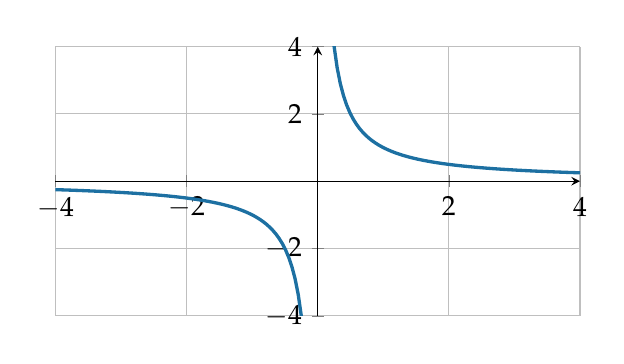
\begin{tikzpicture}\begin{axis}[width=.68\textwidth,height=5cm,axis lines=middle,xmin=-4,xmax=4,ymin=-4,ymax=4,grid=major]\addplot[Blue,very thick,samples=80,domain=-4:-.15]{1/x};\addplot[Blue,very thick,samples=80,domain=.15:4]{1/x};\end{axis}\end{tikzpicture}\end{center}
\end{activite}
\enseignant{$g'(x)=\dfrac{(x-3)(x+3)}{x^2}$; minimum $g(3)=6$; $g(x)$ tends to $+\infty$ at $0^+$ and at $+\infty$. Have students say aloud which piece of data triggers the choice of method.}

\begin{traceecrite}A full study includes: domain, derivative, sign, variations, limits or behaviour at the boundaries, key points and a consistent graph.\end{traceecrite}

\begin{exemple}
Revisit the data from the investigation and write up the solution in order: definition of the objects, property used, exact or approximate calculation, then a concluding sentence. The model answer appears in the teacher edition.
\end{exemple}
\enseignant{$g'(x)=\dfrac{(x-3)(x+3)}{x^2}$; minimum $g(3)=6$; $g(x)$ tends to $+\infty$ at $0^+$ and at $+\infty$.}

\begin{exercice}[-- essential]
\begin{enumerate}\item Give the domain and the asymptotes of $f(x)=6+\dfrac{8}x$.\item Calculate $f'(x)$ and study its sign.\item Study the function $g(x)=x+\dfrac{36}x$ on $]0,+\infty[$.\end{enumerate}
\end{exercice}
\enseignant{The domain is $\R\setminus\{0\}$; asymptotes $x=0$ and $y=6$. $f'(x)=-\dfrac{8}{x^2}<0$. For $g$, $g'(x)=1-\dfrac{36}{x^2}$ and the minimum is reached at $x=6$, with value $12$.}

\manuelref{Calao, pp. 98--103}
\CalaoSession{29}

\begin{dm}Redo practice exercise 2 with the following data: replace the initial value by $265$ and the rate or common ratio by $7$. Write it up in four lines: data, formula, calculation, conclusion.\end{dm}
\enseignant{The answer depends on the exercise revisited. Check above all the consistency of the model, the number of iterations, the rounding and the concluding sentence.}

\begin{sortie}On a half-sheet: write the main rule of the session, work through a very short example and state your confidence level from 1 to 4. Key question(s) of the day: 1, 2 and 3.\end{sortie}

\ifprof
\begin{methode}
\textbf{1 h session:} 7 min of fluency; 10 min of pooling and written record; 28 min of essential exercises; 5 min of correction; 3 min of exit ticket.\\
\textbf{2 h session:} add 20 min of investigation, 20 min of formalisation, a second independent exercise and 10 min of comparative correction.\\
\textbf{Differentiation:} give struggling students a four-box sheet (data, model, calculation, conclusion). Ask quick students to produce a counterexample, a justification or a second method.
\end{methode}
\fi
\sessionheader{30}{21 Jan 2027}{B: 1 h -- C: 2 h}{Review and assessment}{Reciprocal (inverse) function}
\begin{objectifs}\begin{itemize}\item Use domain, derivative and sign.\item Write up a study.\item Correct work methodically.\end{itemize}\end{objectifs}
\begin{automatismes}\begin{enumerate}\item Calculate $5\,\%$ of $100$. \rep{$5$}\item Solve $(x-2)(x+1)=0$. \rep{$x=-1$ or $x=2$}\item Give the excluded value of $\dfrac{x+1}{x}$. \rep{$x=0$}\item Calculate $\dfrac1{5}$ and $\dfrac1{-5}$. \rep{$\dfrac1{5}$ and $-\dfrac1{5}$}\item Differentiate $3x^2-5x+1$. \rep{$6x-5$}\end{enumerate}\end{automatismes}
\begin{prerequis}Reread the last written record and be able to carry out the basic calculations needed today. Before the investigation, have students rephrase the key words: use domain, derivative and sign and write up a study.\end{prerequis}

\begin{activite}
Correct a deliberately flawed study of $h(x)=x+\dfrac4x$: stated domain $\R$, derivative $1+\dfrac4{x^2}$, table with no break at $0$. Rewrite a complete solution.

\end{activite}
\enseignant{The domain is $\R\setminus\{0\}$ and $h'(x)=1-\dfrac4{x^2}$. The table is split at $0$ and takes into account $-2$ and $2$. Have students say aloud which piece of data triggers the choice of method.}

\begin{traceecrite}Check the four items separately: domain, expression of the derivative, sign of the derivative, variations. An error at one step must not hide the following ones.\end{traceecrite}

\begin{exemple}
Revisit the data from the investigation and write up the solution in order: definition of the objects, property used, exact or approximate calculation, then a concluding sentence. The model answer appears in the teacher edition.
\end{exemple}
\enseignant{The domain is $\R\setminus\{0\}$ and $h'(x)=1-\dfrac4{x^2}$. The table is split at $0$ and takes into account $-2$ and $2$.}

\begin{exercice}[-- essential]
\begin{enumerate}\item Give the domain and the asymptotes of $f(x)=2+\dfrac{4}x$.\item Calculate $f'(x)$ and study its sign.\item Study the function $g(x)=x+\dfrac{4}x$ on $]0,+\infty[$.\end{enumerate}
\end{exercice}
\enseignant{The domain is $\R\setminus\{0\}$; asymptotes $x=0$ and $y=2$. $f'(x)=-\dfrac{4}{x^2}<0$. For $g$, $g'(x)=1-\dfrac{4}{x^2}$ and the minimum is reached at $x=2$, with value $4$.}

\manuelref{Calao, pp. 100--103}
\CalaoSession{30}

\begin{dm}Redo practice exercise 3 with the following data: replace the initial value by $270$ and the rate or common ratio by $2$. Write it up in four lines: data, formula, calculation, conclusion.\end{dm}
\enseignant{The answer depends on the exercise revisited. Check above all the consistency of the model, the number of iterations, the rounding and the concluding sentence.}

\begin{sortie}On a half-sheet: write the main rule of the session, work through a very short example and state your confidence level from 1 to 4. Key question(s) of the day: 1 and 2.\end{sortie}

\ifprof
\begin{methode}
\textbf{1 h session:} 7 min of fluency; 10 min of pooling and written record; 28 min of essential exercises; 5 min of correction; 3 min of exit ticket.\\
\textbf{2 h session:} add 20 min of investigation, 20 min of formalisation, a second independent exercise and 10 min of comparative correction.\\
\textbf{Differentiation:} give struggling students a four-box sheet (data, model, calculation, conclusion). Ask quick students to produce a counterexample, a justification or a second method.
\end{methode}
\fi


\chapter{Bivariate statistics}
\competences{represent, choose a linear regression, interpolate, extrapolate with caution, communicate}
\section{Reference course}
A bivariate data set consists of pairs $(x_i,y_i)$. The scatter plot shows a trend, the spread and any outliers.

\begin{center}
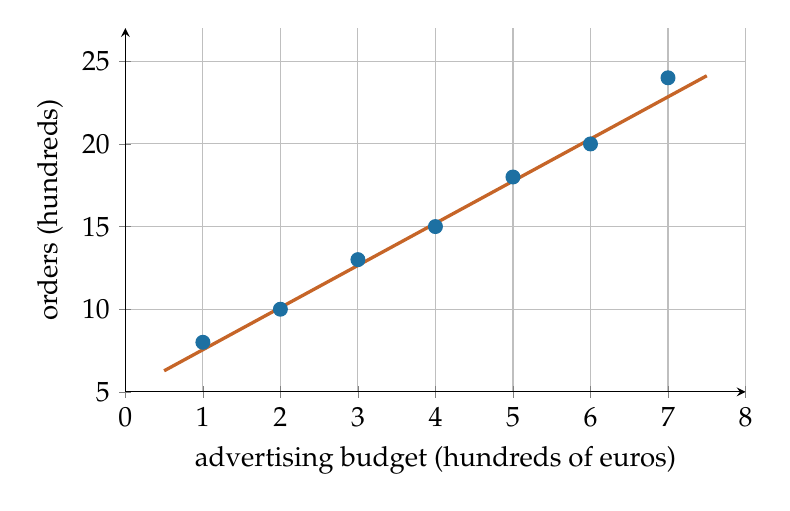
\begin{tikzpicture}
\begin{axis}[width=.78\textwidth,height=6.2cm,axis lines=left,xmin=0,xmax=8,ymin=5,ymax=27,grid=major,xlabel={advertising budget (hundreds of euros)},ylabel={orders (hundreds)}]
\addplot[only marks,mark=*,Blue,mark size=2.5pt] coordinates {(1,8)(2,10)(3,13)(4,15)(5,18)(6,20)(7,24)};
\addplot[Orange,very thick,domain=.5:7.5]{2.55*x+5};
\end{axis}
\end{tikzpicture}
\end{center}

\begin{retenir}
A line of best fit $y=ax+b$ gives estimates, not exact equalities. The coefficient $a$ describes the estimated average change in $y$ when $x$ increases by one unit. Interpolation stays within the range of observed values; extrapolation goes outside that range and must be presented with caution.
\end{retenir}

The mean point $G(\bar x,\bar y)$ has coordinates $\bar x=\dfrac{x_1+\cdots+x_n}{n}$ and $\bar y=\dfrac{y_1+\cdots+y_n}{n}$. A regression line obtained with a calculator passes through $G$, up to rounding.

\begin{methode}
To use $y=ax+b$: 1) replace $x$ by the requested value to estimate $y$; 2) solve $ax+b=y_0$ to estimate $x$; 3) round according to the context; 4) state whether it is interpolation or extrapolation; 5) remind that the result depends on the model.
\end{methode}

A change of variable, for example $z=\log(y)$ or $z=\dfrac1y$, can make a scatter plot roughly linear. We then fit $(x,z)$, and afterwards return to the variable $y$.

\sessionheader{31}{26 Jan 2027}{B: 2 h -- C: 1 h}{Scatter plot}{Bivariate statistics}
\begin{objectifs}\begin{itemize}\item Construct a scatter plot.\item Choose the scales.\item Identify the variables.\end{itemize}\end{objectifs}
\begin{automatismes}\begin{enumerate}\item Write the multiplier for a $10\,\%$ increase. \rep{$1+\dfrac{10}{100}=1.10$}\item Solve $3x+4=25$. \rep{$x=7$}\item Calculate the mean of $6$, $8$ and $10$. \rep{$8$}\item Give the slope between $(1,3)$ and $(4,9)$. \rep{$\dfrac{9-3}{4-1}=2$}\item With $y=2x+5$, calculate $y$ for $x=7$. \rep{$19$}\end{enumerate}\end{automatismes}
\begin{prerequis}Reread the last written record and be able to carry out the basic calculations used today. Before the investigation, have the keywords restated: construct a scatter plot and choose the scales.\end{prerequis}

\begin{activite}
The table $(x_i,y_i)$ gives the advertising spending and the sales over six months: $(1,12),(2,15),(3,17),(4,22),(5,24),(6,28)$. Choose scales, draw the scatter plot and plot the mean point.
\begin{center}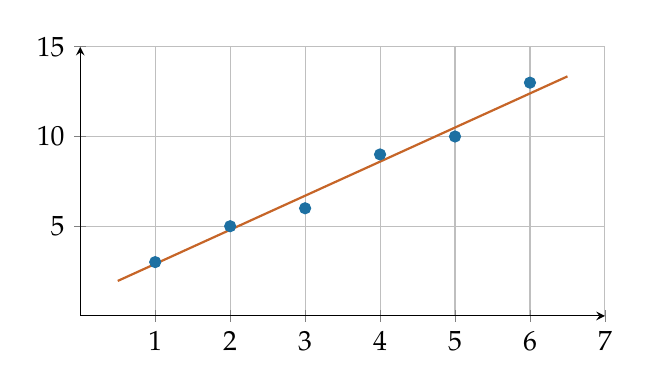
\begin{tikzpicture}\begin{axis}[width=.68\textwidth,height=5cm,axis lines=middle,xmin=0,xmax=7,ymin=0,ymax=15,grid=major]\addplot[only marks,Blue,mark=*] coordinates {(1,3)(2,5)(3,6)(4,9)(5,10)(6,13)};\addplot[Orange,thick,domain=.5:6.5]{1.9*x+1};\end{axis}\end{tikzpicture}\end{center}
\end{activite}
\enseignant{$\bar x=3.5$ and $\bar y=19.67$ approximately. The scatter plot shows an increasing, roughly linear trend. Have students verbalise the piece of data that triggers the choice of method.}

\begin{traceecrite}A scatter plot represents the pairs $(x_i,y_i)$. The axes, units and scales must be indicated; each pair gives a single point.\end{traceecrite}

\begin{exemple}
Take the data of the investigation and write the solution in order: definition of the objects, property used, exact or approximate calculation, then a sentence giving the answer. The model answer appears in the teacher edition.
\end{exemple}
\enseignant{$\bar x=3.5$ and $\bar y=19.67$ approximately. The scatter plot shows an increasing, roughly linear trend.}

\begin{exercice}[-- essential]
\begin{enumerate}\item For $y=3x+13$, estimate $y$ when $x=8$.\item Solve $3x+13=50$.\item The model was built on $[2,12]$: classify the estimates for $x=8$ and $x=30$.\end{enumerate}
\end{exercice}
\enseignant{For $x=8$, $y=37$. The equation gives $x=\dfrac{37}{3}$. $x=8$ gives an interpolation; $x=30$ an extrapolation.}

\manuelref{Calao, course pp. 110--113; exercises p. 114, nos.~1--6}
\CalaoSession{31}

\begin{dm}Redo practice exercise 2 with the following data: replace the initial value with $275$ and the rate or ratio with $3$. Write it up in four lines: data, formula, calculation, conclusion.\end{dm}
\enseignant{The solution depends on the exercise redone. Check above all the consistency of the model, the number of iterations, the rounding and the concluding sentence.}

\begin{sortie}On a half-sheet: write the main rule of the session, work through a very short example and indicate your confidence level from 1 to 4. Key question(s) of the day: 1, 2 and 3.\end{sortie}

\ifprof
\begin{methode}
\textbf{One-hour plan:} 7 min of fluency; 10 min of pooling and written record; 28 min of essential exercises; 5 min of correction; 3 min of exit ticket.\\
\textbf{Two-hour plan:} add 20 min of investigation, 20 min of formalisation, a second independent exercise and 10 min of comparative correction.\\
\textbf{Differentiation:} give struggling students a four-box sheet (data, model, calculation, conclusion). Ask fast students to produce a counterexample, a justification or a second method.
\end{methode}
\fi
\sessionheader{32}{28 Jan 2027}{B: 1 h -- C: 2 h}{Reading and interpreting a scatter plot}{Bivariate statistics}
\begin{objectifs}\begin{itemize}\item Describe a trend.\item Spot spread and outliers.\item Avoid unwarranted causality.\end{itemize}\end{objectifs}
\begin{automatismes}\begin{enumerate}\item Simplify $3x+7-x+2$. \rep{$2x+9$}\item Calculate the mean of $7$, $9$ and $11$. \rep{$9$}\item Give the slope between $(1,3)$ and $(4,9)$. \rep{$\dfrac{9-3}{4-1}=2$}\item With $y=2x+5$, calculate $y$ for $x=7$. \rep{$19$}\item Solve $3x+4=25$. \rep{$x=7$}\end{enumerate}\end{automatismes}
\begin{prerequis}Reread the last written record and be able to carry out the basic calculations used today. Before the investigation, have the keywords restated: describe a trend and spot spread and outliers.\end{prerequis}

\begin{activite}
Compare three scatter plots: a tight increasing trend, a scattered decreasing trend, no trend. For each, write two sentences without using the word ``cause''.

\end{activite}
\enseignant{The description covers direction, shape, spread and outliers. A scatter plot alone does not establish causality. Have students verbalise the piece of data that triggers the choice of method.}

\begin{traceecrite}Describing a scatter plot means commenting on its direction, shape, spread and outliers, without claiming a causality that has not been established.\end{traceecrite}

\begin{exemple}
Take the data of the investigation and write the solution in order: definition of the objects, property used, exact or approximate calculation, then a sentence giving the answer. The model answer appears in the teacher edition.
\end{exemple}
\enseignant{The description covers direction, shape, spread and outliers. A scatter plot alone does not establish causality.}

\begin{exercice}[-- essential]
\begin{enumerate}\item For $y=4x+14$, estimate $y$ when $x=8$.\item Solve $4x+14=50$.\item The model was built on $[2,12]$: classify the estimates for $x=8$ and $x=30$.\end{enumerate}
\end{exercice}
\enseignant{For $x=8$, $y=46$. The equation gives $x=\dfrac{36}{4}$. $x=8$ gives an interpolation; $x=30$ an extrapolation.}

\manuelref{Calao, p. 116, nos.~11--15}
\CalaoSession{32}

\begin{dm}Redo practice exercise 3 with the following data: replace the initial value with $280$ and the rate or ratio with $4$. Write it up in four lines: data, formula, calculation, conclusion.\end{dm}
\enseignant{The solution depends on the exercise redone. Check above all the consistency of the model, the number of iterations, the rounding and the concluding sentence.}

\begin{sortie}On a half-sheet: write the main rule of the session, work through a very short example and indicate your confidence level from 1 to 4. Key question(s) of the day: 1 and 2.\end{sortie}

\ifprof
\begin{methode}
\textbf{One-hour plan:} 7 min of fluency; 10 min of pooling and written record; 28 min of essential exercises; 5 min of correction; 3 min of exit ticket.\\
\textbf{Two-hour plan:} add 20 min of investigation, 20 min of formalisation, a second independent exercise and 10 min of comparative correction.\\
\textbf{Differentiation:} give struggling students a four-box sheet (data, model, calculation, conclusion). Ask fast students to produce a counterexample, a justification or a second method.
\end{methode}
\fi
\sessionheader{33}{2 Feb 2027}{B: 2 h -- C: 1 h}{Linear regression}{Bivariate statistics}
\begin{objectifs}\begin{itemize}\item Obtain a linear regression.\item Interpret $a$ and $b$.\item Check with the mean point.\end{itemize}\end{objectifs}
\begin{automatismes}\begin{enumerate}\item Calculate $20\,\%$ of $160$. \rep{$32$}\item Give the slope between $(1,3)$ and $(4,9)$. \rep{$\dfrac{9-3}{4-1}=2$}\item With $y=2x+5$, calculate $y$ for $x=7$. \rep{$19$}\item Solve $3x+4=25$. \rep{$x=7$}\item Calculate the mean of $8$, $10$ and $12$. \rep{$10$}\end{enumerate}\end{automatismes}
\begin{prerequis}Reread the last written record and be able to carry out the basic calculations used today. Before the investigation, have the keywords restated: obtain a linear regression and interpret $a$ and $b$.\end{prerequis}

\begin{activite}
With the data of session 31, obtain the linear regression with a calculator. Interpret the slope and check that the mean point lies approximately on the line.
\begin{center}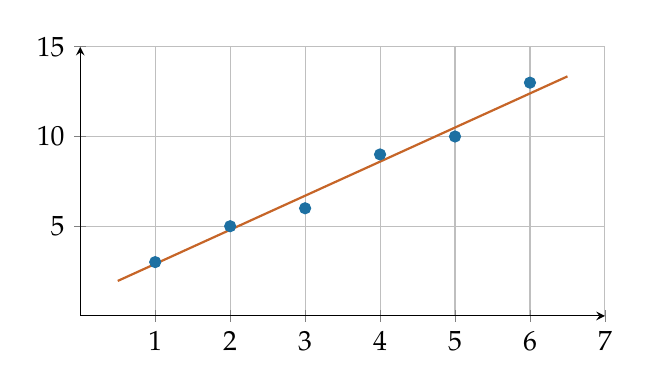
\begin{tikzpicture}\begin{axis}[width=.68\textwidth,height=5cm,axis lines=middle,xmin=0,xmax=7,ymin=0,ymax=15,grid=major]\addplot[only marks,Blue,mark=*] coordinates {(1,3)(2,5)(3,6)(4,9)(5,10)(6,13)};\addplot[Orange,thick,domain=.5:6.5]{1.9*x+1};\end{axis}\end{tikzpicture}\end{center}
\end{activite}
\enseignant{A regression gives approximately $y=3.17x+8.57$. An extra hundred euros is associated with about $317$ extra sales if $y$ is in hundreds. Have students verbalise the piece of data that triggers the choice of method.}

\begin{traceecrite}A line $y=ax+b$ fits a scatter plot. $a$ represents the estimated average change in $y$ for one extra unit of $x$.\end{traceecrite}

\begin{exemple}
Take the data of the investigation and write the solution in order: definition of the objects, property used, exact or approximate calculation, then a sentence giving the answer. The model answer appears in the teacher edition.
\end{exemple}
\enseignant{A regression gives approximately $y=3.17x+8.57$. An extra hundred euros is associated with about $317$ extra sales if $y$ is in hundreds.}

\begin{exercice}[-- essential]
\begin{enumerate}\item For $y=5x+15$, estimate $y$ when $x=8$.\item Solve $5x+15=50$.\item The model was built on $[2,12]$: classify the estimates for $x=8$ and $x=30$.\end{enumerate}
\end{exercice}
\enseignant{For $x=8$, $y=55$. The equation gives $x=\dfrac{35}{5}$. $x=8$ gives an interpolation; $x=30$ an extrapolation.}

\manuelref{Calao, course pp. 110--113; exercises p. 117, nos.~16--18}
\CalaoSession{33}

\begin{dm}Redo practice exercise 2 with the following data: replace the initial value with $285$ and the rate or ratio with $5$. Write it up in four lines: data, formula, calculation, conclusion.\end{dm}
\enseignant{The solution depends on the exercise redone. Check above all the consistency of the model, the number of iterations, the rounding and the concluding sentence.}

\begin{sortie}On a half-sheet: write the main rule of the session, work through a very short example and indicate your confidence level from 1 to 4. Key question(s) of the day: 1, 2 and 3.\end{sortie}

\ifprof
\begin{methode}
\textbf{One-hour plan:} 7 min of fluency; 10 min of pooling and written record; 28 min of essential exercises; 5 min of correction; 3 min of exit ticket.\\
\textbf{Two-hour plan:} add 20 min of investigation, 20 min of formalisation, a second independent exercise and 10 min of comparative correction.\\
\textbf{Differentiation:} give struggling students a four-box sheet (data, model, calculation, conclusion). Ask fast students to produce a counterexample, a justification or a second method.
\end{methode}
\fi
\sessionheader{34}{4 Feb 2027}{B: 1 h -- C: 2 h}{Interpolation}{Bivariate statistics}
\begin{objectifs}\begin{itemize}\item Interpolate.\item Solve using the model.\item Express an estimate.\end{itemize}\end{objectifs}
\begin{automatismes}\begin{enumerate}\item Write the multiplier for a $25\,\%$ increase. \rep{$1+\dfrac{25}{100}=1.25$}\item With $y=2x+5$, calculate $y$ for $x=7$. \rep{$19$}\item Solve $3x+4=25$. \rep{$x=7$}\item Calculate the mean of $9$, $11$ and $13$. \rep{$11$}\item Give the slope between $(1,3)$ and $(4,9)$. \rep{$\dfrac{9-3}{4-1}=2$}\end{enumerate}\end{automatismes}
\begin{prerequis}Reread the last written record and be able to carry out the basic calculations used today. Before the investigation, have the keywords restated: interpolate and solve using the model.\end{prerequis}

\begin{activite}
Over the observed period $x\in[1,12]$, the model is $y=2.8x+14$. Estimate $y$ for $x=7.5$, then estimate $x$ when $y=35$. Classify each estimate.
\begin{center}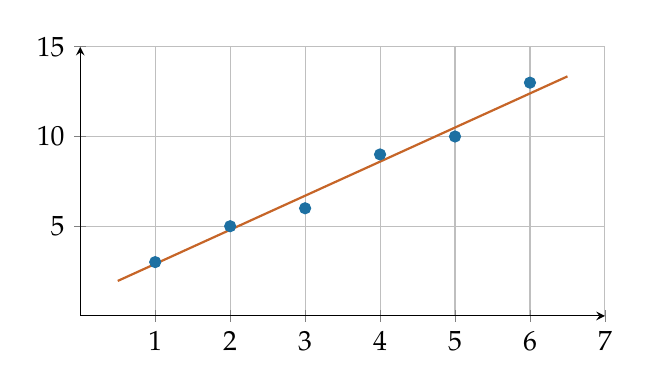
\begin{tikzpicture}\begin{axis}[width=.68\textwidth,height=5cm,axis lines=middle,xmin=0,xmax=7,ymin=0,ymax=15,grid=major]\addplot[only marks,Blue,mark=*] coordinates {(1,3)(2,5)(3,6)(4,9)(5,10)(6,13)};\addplot[Orange,thick,domain=.5:6.5]{1.9*x+1};\end{axis}\end{tikzpicture}\end{center}
\end{activite}
\enseignant{$y=35$ and $x=7.5$. Both values lie inside the observed range: interpolations. Have students verbalise the piece of data that triggers the choice of method.}

\begin{traceecrite}An interpolation estimates a value inside the observed range. The result is an estimate that depends on the model.\end{traceecrite}

\begin{exemple}
Take the data of the investigation and write the solution in order: definition of the objects, property used, exact or approximate calculation, then a sentence giving the answer. The model answer appears in the teacher edition.
\end{exemple}
\enseignant{$y=35$ and $x=7.5$. Both values lie inside the observed range: interpolations.}

\begin{exercice}[-- essential]
\begin{enumerate}\item For $y=6x+16$, estimate $y$ when $x=8$.\item Solve $6x+16=50$.\item The model was built on $[2,12]$: classify the estimates for $x=8$ and $x=30$.\end{enumerate}
\end{exercice}
\enseignant{For $x=8$, $y=64$. The equation gives $x=\dfrac{34}{6}$. $x=8$ gives an interpolation; $x=30$ an extrapolation.}

\manuelref{Calao, p. 118, nos.~19--24}
\CalaoSession{34}

\begin{dm}Redo practice exercise 3 with the following data: replace the initial value with $290$ and the rate or ratio with $6$. Write it up in four lines: data, formula, calculation, conclusion.\end{dm}
\enseignant{The solution depends on the exercise redone. Check above all the consistency of the model, the number of iterations, the rounding and the concluding sentence.}

\begin{sortie}On a half-sheet: write the main rule of the session, work through a very short example and indicate your confidence level from 1 to 4. Key question(s) of the day: 1 and 2.\end{sortie}

\ifprof
\begin{methode}
\textbf{One-hour plan:} 7 min of fluency; 10 min of pooling and written record; 28 min of essential exercises; 5 min of correction; 3 min of exit ticket.\\
\textbf{Two-hour plan:} add 20 min of investigation, 20 min of formalisation, a second independent exercise and 10 min of comparative correction.\\
\textbf{Differentiation:} give struggling students a four-box sheet (data, model, calculation, conclusion). Ask fast students to produce a counterexample, a justification or a second method.
\end{methode}
\fi
\sessionheader{35}{9 Feb 2027}{B: 2 h -- C: 1 h}{Extrapolation}{Bivariate statistics}
\begin{objectifs}\begin{itemize}\item Extrapolate with caution.\item Assess plausibility.\item Present a limitation of the model.\end{itemize}\end{objectifs}
\begin{automatismes}\begin{enumerate}\item Simplify $3x+3-x+2$. \rep{$2x+5$}\item Solve $3x+4=25$. \rep{$x=7$}\item Calculate the mean of $3$, $5$ and $7$. \rep{$5$}\item Give the slope between $(1,3)$ and $(4,9)$. \rep{$\dfrac{9-3}{4-1}=2$}\item With $y=2x+5$, calculate $y$ for $x=7$. \rep{$19$}\end{enumerate}\end{automatismes}
\begin{prerequis}Reread the last written record and be able to carry out the basic calculations used today. Before the investigation, have the keywords restated: extrapolate with caution and assess plausibility.\end{prerequis}

\begin{activite}
The same model $y=2.8x+14$, fitted on $[1,12]$, is used for $x=40$. Calculate the estimate, then give three reasons why it may be unreliable.
\begin{center}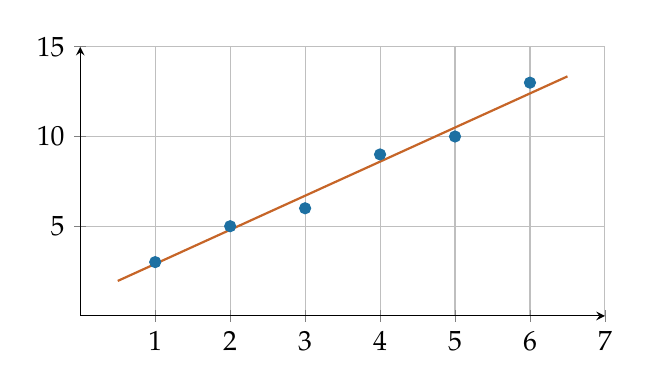
\begin{tikzpicture}\begin{axis}[width=.68\textwidth,height=5cm,axis lines=middle,xmin=0,xmax=7,ymin=0,ymax=15,grid=major]\addplot[only marks,Blue,mark=*] coordinates {(1,3)(2,5)(3,6)(4,9)(5,10)(6,13)};\addplot[Orange,thick,domain=.5:6.5]{1.9*x+1};\end{axis}\end{tikzpicture}\end{center}
\end{activite}
\enseignant{The estimate is $126$. It is far from the data, the trend may change and real-world constraints may cap the variable. Have students verbalise the piece of data that triggers the choice of method.}

\begin{traceecrite}An extrapolation estimates outside the observed range. The further away we go, the more caution is needed.\end{traceecrite}

\begin{exemple}
Take the data of the investigation and write the solution in order: definition of the objects, property used, exact or approximate calculation, then a sentence giving the answer. The model answer appears in the teacher edition.
\end{exemple}
\enseignant{The estimate is $126$. It is far from the data, the trend may change and real-world constraints may cap the variable.}

\begin{exercice}[-- essential]
\begin{enumerate}\item For $y=2x+12$, estimate $y$ when $x=8$.\item Solve $2x+12=50$.\item The model was built on $[2,12]$: classify the estimates for $x=8$ and $x=30$.\end{enumerate}
\end{exercice}
\enseignant{For $x=8$, $y=28$. The equation gives $x=\dfrac{38}{2}$. $x=8$ gives an interpolation; $x=30$ an extrapolation.}

\manuelref{Calao, p. 119, nos.~25--27}
\CalaoSession{35}

\begin{dm}Redo practice exercise 2 with the following data: replace the initial value with $295$ and the rate or ratio with $7$. Write it up in four lines: data, formula, calculation, conclusion.\end{dm}
\enseignant{The solution depends on the exercise redone. Check above all the consistency of the model, the number of iterations, the rounding and the concluding sentence.}

\begin{sortie}On a half-sheet: write the main rule of the session, work through a very short example and indicate your confidence level from 1 to 4. Key question(s) of the day: 1, 2 and 3.\end{sortie}

\ifprof
\begin{methode}
\textbf{One-hour plan:} 7 min of fluency; 10 min of pooling and written record; 28 min of essential exercises; 5 min of correction; 3 min of exit ticket.\\
\textbf{Two-hour plan:} add 20 min of investigation, 20 min of formalisation, a second independent exercise and 10 min of comparative correction.\\
\textbf{Differentiation:} give struggling students a four-box sheet (data, model, calculation, conclusion). Ask fast students to produce a counterexample, a justification or a second method.
\end{methode}
\fi
\sessionheader{36}{11 Feb 2027}{B: 1 h -- C: 2 h}{Change of variable}{Bivariate statistics}
\begin{objectifs}\begin{itemize}\item Carry out a change of variable.\item Fit the new data.\item Return to the original variable.\end{itemize}\end{objectifs}
\begin{automatismes}\begin{enumerate}\item Calculate $5\,\%$ of $80$. \rep{$4$}\item Calculate the mean of $4$, $6$ and $8$. \rep{$6$}\item Give the slope between $(1,3)$ and $(4,9)$. \rep{$\dfrac{9-3}{4-1}=2$}\item With $y=2x+5$, calculate $y$ for $x=7$. \rep{$19$}\item Solve $3x+4=25$. \rep{$x=7$}\end{enumerate}\end{automatismes}
\begin{prerequis}Reread the last written record and be able to carry out the basic calculations used today. Before the investigation, have the keywords restated: carry out a change of variable and fit the new data.\end{prerequis}

\begin{activite}
The data appear to be exponential. We set $z=\log(y)$ and the fit gives $z=0.08x+1.2$. Express $y$ as a function of $x$, then calculate $y$ for $x=5$.

\end{activite}
\enseignant{$y=10^{0.08x+1.2}$. For $x=5$, $y=10^{1.6}\approx39.8$. Have students verbalise the piece of data that triggers the choice of method.}

\begin{traceecrite}A change of variable can make a scatter plot linear. After fitting in the new variable, we must return to the original variable.\end{traceecrite}

\begin{exemple}
Take the data of the investigation and write the solution in order: definition of the objects, property used, exact or approximate calculation, then a sentence giving the answer. The model answer appears in the teacher edition.
\end{exemple}
\enseignant{$y=10^{0.08x+1.2}$. For $x=5$, $y=10^{1.6}\approx39.8$.}

\begin{exercice}[-- essential]
\begin{enumerate}\item For $y=3x+13$, estimate $y$ when $x=8$.\item Solve $3x+13=50$.\item The model was built on $[2,12]$: classify the estimates for $x=8$ and $x=30$.\end{enumerate}
\end{exercice}
\enseignant{For $x=8$, $y=37$. The equation gives $x=\dfrac{37}{3}$. $x=8$ gives an interpolation; $x=30$ an extrapolation.}

\manuelref{Calao, p. 120, nos.~28--29}
\CalaoSession{36}

\begin{dm}Redo practice exercise 3 with the following data: replace the initial value with $300$ and the rate or ratio with $2$. Write it up in four lines: data, formula, calculation, conclusion.\end{dm}
\enseignant{The solution depends on the exercise redone. Check above all the consistency of the model, the number of iterations, the rounding and the concluding sentence.}

\begin{sortie}On a half-sheet: write the main rule of the session, work through a very short example and indicate your confidence level from 1 to 4. Key question(s) of the day: 1 and 2.\end{sortie}

\ifprof
\begin{methode}
\textbf{One-hour plan:} 7 min of fluency; 10 min of pooling and written record; 28 min of essential exercises; 5 min of correction; 3 min of exit ticket.\\
\textbf{Two-hour plan:} add 20 min of investigation, 20 min of formalisation, a second independent exercise and 10 min of comparative correction.\\
\textbf{Differentiation:} give struggling students a four-box sheet (data, model, calculation, conclusion). Ask fast students to produce a counterexample, a justification or a second method.
\end{methode}
\fi
\sessionheader{37}{2 Mar 2027}{B: 2 h -- C: 1 h}{Choosing the model and fitting}{Bivariate statistics}
\begin{objectifs}\begin{itemize}\item Compare models.\item Use residuals.\item Define a range of use.\end{itemize}\end{objectifs}
\begin{automatismes}\begin{enumerate}\item Write the multiplier for a $10\,\%$ increase. \rep{$1+\dfrac{10}{100}=1.10$}\item Give the slope between $(1,3)$ and $(4,9)$. \rep{$\dfrac{9-3}{4-1}=2$}\item With $y=2x+5$, calculate $y$ for $x=7$. \rep{$19$}\item Solve $3x+4=25$. \rep{$x=7$}\item Calculate the mean of $5$, $7$ and $9$. \rep{$7$}\end{enumerate}\end{automatismes}
\begin{prerequis}Reread the last written record and be able to carry out the basic calculations used today. Before the investigation, have the keywords restated: compare models and use residuals.\end{prerequis}

\begin{activite}
Two models give total absolute residuals of $18.4$ and $11.7$ over the observed range. The second, however, shows unrealistic growth beyond $x=20$. Choose a model to interpolate at $x=12$, then discuss extrapolation at $x=50$.
\begin{center}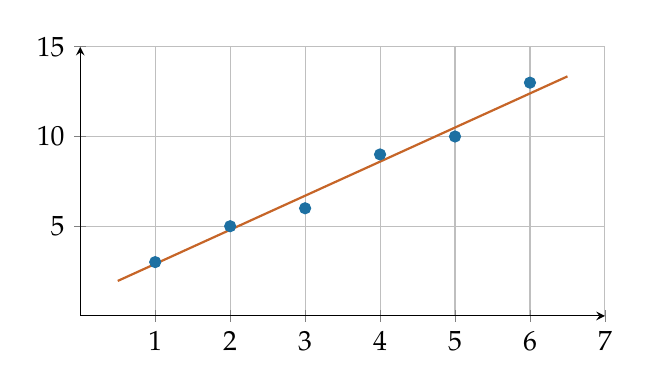
\begin{tikzpicture}\begin{axis}[width=.68\textwidth,height=5cm,axis lines=middle,xmin=0,xmax=7,ymin=0,ymax=15,grid=major]\addplot[only marks,Blue,mark=*] coordinates {(1,3)(2,5)(3,6)(4,9)(5,10)(6,13)};\addplot[Orange,thick,domain=.5:6.5]{1.9*x+1};\end{axis}\end{tikzpicture}\end{center}
\end{activite}
\enseignant{The second is preferable for interpolating over the observed range if the other criteria are comparable; no automatic choice is justified for $x=50$. Have students verbalise the piece of data that triggers the choice of method.}

\begin{traceecrite}We choose a model according to the shape of the scatter plot, the size of the residuals and the range of use. A better visual fit does not allow unlimited extrapolation.\end{traceecrite}

\begin{exemple}
Take the data of the investigation and write the solution in order: definition of the objects, property used, exact or approximate calculation, then a sentence giving the answer. The model answer appears in the teacher edition.
\end{exemple}
\enseignant{The second is preferable for interpolating over the observed range if the other criteria are comparable; no automatic choice is justified for $x=50$.}

\begin{exercice}[-- essential]
\begin{enumerate}\item For $y=4x+14$, estimate $y$ when $x=8$.\item Solve $4x+14=50$.\item The model was built on $[2,12]$: classify the estimates for $x=8$ and $x=30$.\end{enumerate}
\end{exercice}
\enseignant{For $x=8$, $y=46$. The equation gives $x=\dfrac{36}{4}$. $x=8$ gives an interpolation; $x=30$ an extrapolation.}

\manuelref{Calao, p. 121, nos.~30--32, then p. 122, no.~33}
\CalaoSession{37}

\begin{dm}Redo practice exercise 2 with the following data: replace the initial value with $305$ and the rate or ratio with $3$. Write it up in four lines: data, formula, calculation, conclusion.\end{dm}
\enseignant{The solution depends on the exercise redone. Check above all the consistency of the model, the number of iterations, the rounding and the concluding sentence.}

\begin{sortie}On a half-sheet: write the main rule of the session, work through a very short example and indicate your confidence level from 1 to 4. Key question(s) of the day: 1, 2 and 3.\end{sortie}

\ifprof
\begin{methode}
\textbf{One-hour plan:} 7 min of fluency; 10 min of pooling and written record; 28 min of essential exercises; 5 min of correction; 3 min of exit ticket.\\
\textbf{Two-hour plan:} add 20 min of investigation, 20 min of formalisation, a second independent exercise and 10 min of comparative correction.\\
\textbf{Differentiation:} give struggling students a four-box sheet (data, model, calculation, conclusion). Ask fast students to produce a counterexample, a justification or a second method.
\end{methode}
\fi
\sessionheader{38}{4 Mar 2027}{B: 1 h -- C: 2 h}{Review and assessment}{Bivariate statistics}
\begin{objectifs}\begin{itemize}\item Choose and use a regression.\item Write a statistical conclusion.\item Analyse an error.\end{itemize}\end{objectifs}
\begin{automatismes}\begin{enumerate}\item Simplify $3x+6-x+2$. \rep{$2x+8$}\item With $y=2x+5$, calculate $y$ for $x=7$. \rep{$19$}\item Solve $3x+4=25$. \rep{$x=7$}\item Calculate the mean of $6$, $8$ and $10$. \rep{$8$}\item Give the slope between $(1,3)$ and $(4,9)$. \rep{$\dfrac{9-3}{4-1}=2$}\end{enumerate}\end{automatismes}
\begin{prerequis}Reread the last written record and be able to carry out the basic calculations used today. Before the investigation, have the keywords restated: choose and use a regression and write a statistical conclusion.\end{prerequis}

\begin{activite}
Starting from a scatter plot supplied by the teacher, produce a complete answer: choice of model, equation, estimate, type of estimate, unit and caveat. Swap papers and use a six-criterion grid.

\end{activite}
\enseignant{The marking checks the consistency of the model and the presence of the six required elements, not only the numerical result. Have students verbalise the piece of data that triggers the choice of method.}

\begin{traceecrite}A complete statistical answer contains the model, the calculation, the rounding, the unit, the type of estimate and a caveat on validity.\end{traceecrite}

\begin{exemple}
Take the data of the investigation and write the solution in order: definition of the objects, property used, exact or approximate calculation, then a sentence giving the answer. The model answer appears in the teacher edition.
\end{exemple}
\enseignant{The marking checks the consistency of the model and the presence of the six required elements, not only the numerical result.}

\begin{exercice}[-- essential]
\begin{enumerate}\item For $y=5x+15$, estimate $y$ when $x=8$.\item Solve $5x+15=50$.\item The model was built on $[2,12]$: classify the estimates for $x=8$ and $x=30$.\end{enumerate}
\end{exercice}
\enseignant{For $x=8$, $y=55$. The equation gives $x=\dfrac{35}{5}$. $x=8$ gives an interpolation; $x=30$ an extrapolation.}

\manuelref{Calao, pp. 122--123}
\CalaoSession{38}

\begin{dm}Redo practice exercise 3 with the following data: replace the initial value with $310$ and the rate or ratio with $4$. Write it up in four lines: data, formula, calculation, conclusion.\end{dm}
\enseignant{The solution depends on the exercise redone. Check above all the consistency of the model, the number of iterations, the rounding and the concluding sentence.}

\begin{sortie}On a half-sheet: write the main rule of the session, work through a very short example and indicate your confidence level from 1 to 4. Key question(s) of the day: 1 and 2.\end{sortie}

\ifprof
\begin{methode}
\textbf{One-hour plan:} 7 min of fluency; 10 min of pooling and written record; 28 min of essential exercises; 5 min of correction; 3 min of exit ticket.\\
\textbf{Two-hour plan:} add 20 min of investigation, 20 min of formalisation, a second independent exercise and 10 min of comparative correction.\\
\textbf{Differentiation:} give struggling students a four-box sheet (data, model, calculation, conclusion). Ask fast students to produce a counterexample, a justification or a second method.
\end{methode}
\fi


\chapter{Conditional probability}
\competences{model with a tree or a table, calculate, reason about independence, interpret}
\section{Reference course}
For two events $A$ and $B$ with $P(A)>0$, the probability of $B$ given $A$ is
\[
P_A(B)=P(B\mid A)=\frac{P(A\cap B)}{P(A)}.
\]

\begin{center}
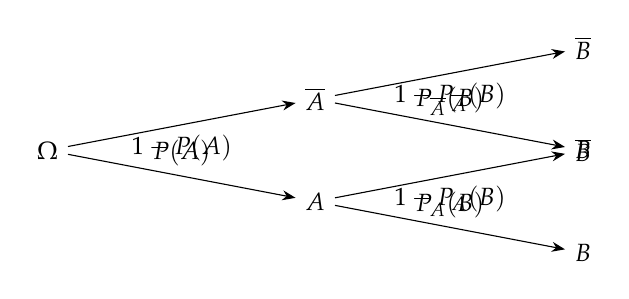
\begin{tikzpicture}[grow=right,level distance=34mm,sibling distance=13mm,every node/.style={font=\small},edge from parent/.style={draw,-{Stealth}}]
\node {$\Omega$}
 child {node {$A$}
   child {node {$B$} edge from parent node[above] {$P_A(B)$}}
   child {node {$\overline B$} edge from parent node[below] {$1-P_A(B)$}}
   edge from parent node[above] {$P(A)$}}
 child {node {$\overline A$}
   child {node {$B$} edge from parent node[above] {$P_{\overline A}(B)$}}
   child {node {$\overline B$} edge from parent node[below] {$1-P_{\overline A}(B)$}}
   edge from parent node[below] {$1-P(A)$}};
\end{tikzpicture}
\end{center}

\begin{retenir}
In a weighted tree, the probabilities leaving the same node sum to $1$. We multiply the probabilities along a path: $P(A\cap B)=P(A)P_A(B)$. We add the probabilities of mutually exclusive paths leading to the event we are looking for.
\end{retenir}

If $A_1,\ldots,A_n$ form a partition of the sample space, then
\[
P(B)=P(A_1)P_{A_1}(B)+\cdots+P(A_n)P_{A_n}(B).
\]
Two events $A$ and $B$ with nonzero probabilities are independent if $P(A\cap B)=P(A)P(B)$, or equivalently if $P_A(B)=P(B)$.

\begin{erreur}
Do not confuse $P_A(B)$ and $P_B(A)$. The condition comes after the word ``given'' and is written as a subscript in this notation.
\end{erreur}

\begin{exemple}
$40\,\%$ of customers buy online. Among them, $12\,\%$ return their order; among the others, $5\,\%$ return it. Then $P(R)=0.40\times0.12+0.60\times0.05=0.078$. The overall return rate is therefore $7.8\,\%$.
\end{exemple}

\sessionheader{39}{9 Mar 2027}{B: 2 h -- C: 1 h}{Conditioning}{Conditional probability}
\begin{objectifs}\begin{itemize}\item Define a conditional probability.\item Move from counts to probabilities.\item Interpret.\end{itemize}\end{objectifs}
\begin{automatismes}\begin{enumerate}\item Calculate $20\,\%$ of $140$. \rep{$28$}\item What is the sum of the branches leaving a node? \rep{$1$}\item Calculate $0.7\times0.4$. \rep{$0.28$}\item If $P(A)=0.37$, calculate $P(\overline A)$. \rep{$0.63$}\item Simplify $\dfrac{18}{30}$. \rep{$\dfrac35$}\end{enumerate}\end{automatismes}
\begin{prerequis}Reread the last written record and be able to carry out the basic calculations used today. Before the investigation, have the keywords restated: define a conditional probability and move from counts to probabilities.\end{prerequis}

\begin{activite}
In a survey, $180$ customers out of $600$ use a premium card and $72$ of these $180$ customers buy every week. Calculate $P(P)$, $P(P\cap H)$ and $P_P(H)$, then interpret.

\end{activite}
\enseignant{$P(P)=0.30$, $P(P\cap H)=0.12$ and $P_P(H)=\dfrac{72}{180}=0.40$. Have students verbalise the piece of data that triggers the choice of method.}

\begin{traceecrite}For $P(A)>0$, $P_A(B)=\dfrac{P(A\cap B)}{P(A)}$. This is the probability of $B$ within the population restricted to $A$.\end{traceecrite}

\begin{exemple}
Take the data of the investigation and write the solution in order: definition of the objects, property used, exact or approximate calculation, then a sentence giving the answer. The model answer appears in the teacher edition.
\end{exemple}
\enseignant{$P(P)=0.30$, $P(P\cap H)=0.12$ and $P_P(H)=\dfrac{72}{180}=0.40$.}

\begin{exercice}[-- essential]
\begin{enumerate}\item We know $P(A)=0.35$, $P_A(B)=0.6$ and $P_{\overline A}(B)=0.8$. Construct the tree.\item Calculate $P(A\cap B)$ then $P(B)$.\item Calculate $P_B(A)$ and test independence.\end{enumerate}
\end{exercice}
\enseignant{$P(A\cap B)=0.35\times0.6$. Then $P(B)=P(A)P_A(B)+(1-P(A))P_{\overline A}(B)$ and $P_B(A)=\dfrac{P(A\cap B)}{P(B)}$. Compare with $P(A)$.}

\manuelref{Calao, course pp. 132--137; exercises p. 138, nos.~1--5}
\ExoSession{39}

\begin{dm}Redo practice exercise 2 with the following data: replace the initial value with $315$ and the rate or ratio with $5$. Write it up in four lines: data, formula, calculation, conclusion.\end{dm}
\enseignant{The solution depends on the exercise redone. Check above all the consistency of the model, the number of iterations, the rounding and the concluding sentence.}

\begin{sortie}On a half-sheet: write the main rule of the session, work through a very short example and indicate your confidence level from 1 to 4. Key question(s) of the day: 1, 2 and 3.\end{sortie}

\ifprof
\begin{methode}
\textbf{One-hour plan:} 7 min of fluency; 10 min of pooling and written record; 28 min of essential exercises; 5 min of correction; 3 min of exit ticket.\\
\textbf{Two-hour plan:} add 20 min of investigation, 20 min of formalisation, a second independent exercise and 10 min of comparative correction.\\
\textbf{Differentiation:} give struggling students a four-box sheet (data, model, calculation, conclusion). Ask fast students to produce a counterexample, a justification or a second method.
\end{methode}
\fi
\sessionheader{40}{11 Mar 2027}{B: 1 h -- C: 2 h}{Weighted trees}{Conditional probability}
    \begin{objectifs}\begin{itemize}\item Construct and complete a tree.\item Read a conditional probability.\item Check the sums.\end{itemize}\end{objectifs}
    \begin{automatismes}\begin{enumerate}\item Write the multiplier for a $25\,\%$ increase. \rep{$1+\dfrac{25}{100}=1.25$}\item Calculate $0.8\times0.4$. \rep{$0.32$}\item If $P(A)=0.37$, calculate $P(\overline A)$. \rep{$0.63$}\item Simplify $\dfrac{18}{30}$. \rep{$\dfrac35$}\item What is the sum of the branches leaving a node? \rep{$1$}\end{enumerate}\end{automatismes}
    \begin{prerequis}Reread the last written record and be able to carry out the basic calculations used today. Before the investigation, have the keywords restated: construct and complete a tree and read a conditional probability.\end{prerequis}

    \begin{activite}
    $35\,\%$ of orders are express. Among them, $4\,\%$ are late; among standard orders, $9\,\%$ are late. Construct and complete the tree.
    \begin{center}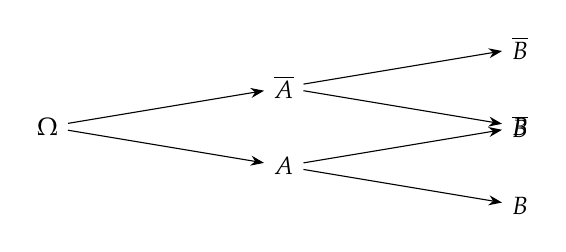
\begin{tikzpicture}[grow=right,level distance=30mm,sibling distance=10mm,every node/.style={font=\small},edge from parent/.style={draw,-{Stealth}}]
\node {$\Omega$} child {node {$A$} child {node {$B$}} child {node {$\overline B$}}} child {node {$\overline A$} child {node {$B$}} child {node {$\overline B$}}};
\end{tikzpicture}\end{center}
    \end{activite}
    \enseignant{First branches: $0.35$ and $0.65$. Then $0.04$ and $0.96$; finally $0.09$ and $0.91$. Have students verbalise the piece of data that triggers the choice of method.}

    \begin{traceecrite}In a tree, the branches leaving a node sum to $1$. The second-level probabilities are conditional.\end{traceecrite}

    \begin{exemple}
    Take the data of the investigation and write the solution in order: definition of the objects, property used, exact or approximate calculation, then a sentence giving the answer. The model answer appears in the teacher edition.
    \end{exemple}
    \enseignant{First branches: $0.35$ and $0.65$. Then $0.04$ and $0.96$; finally $0.09$ and $0.91$.}

    \begin{exercice}[-- essential]
    \begin{enumerate}\item We know $P(A)=0.40$, $P_A(B)=0.2$ and $P_{\overline A}(B)=0.4$. Construct the tree.\item Calculate $P(A\cap B)$ then $P(B)$.\item Calculate $P_B(A)$ and test independence.\end{enumerate}
    \end{exercice}
    \enseignant{$P(A\cap B)=0.40\times0.2$. Then $P(B)=P(A)P_A(B)+(1-P(A))P_{\overline A}(B)$ and $P_B(A)=\dfrac{P(A\cap B)}{P(B)}$. Compare with $P(A)$.}

    \manuelref{Calao, course pp. 133--137; exercises p. 140, nos.~14--18}
\ExoSession{40}

    \begin{dm}Redo practice exercise 3 with the following data: replace the initial value with $320$ and the rate or ratio with $6$. Write it up in four lines: data, formula, calculation, conclusion.\end{dm}
    \enseignant{The solution depends on the exercise redone. Check above all the consistency of the model, the number of iterations, the rounding and the concluding sentence.}

    \begin{sortie}On a half-sheet: write the main rule of the session, work through a very short example and indicate your confidence level from 1 to 4. Key question(s) of the day: 1 and 2.\end{sortie}

    \ifprof
    \begin{methode}
    \textbf{One-hour plan:} 7 min of fluency; 10 min of pooling and written record; 28 min of essential exercises; 5 min of correction; 3 min of exit ticket.\\
    \textbf{Two-hour plan:} add 20 min of investigation, 20 min of formalisation, a second independent exercise and 10 min of comparative correction.\\
    \textbf{Differentiation:} give struggling students a four-box sheet (data, model, calculation, conclusion). Ask fast students to produce a counterexample, a justification or a second method.
    \end{methode}
    \fi
\sessionheader{41}{16 Mar 2027}{B: 2 h -- C: 1 h}{Product of probabilities along a path}{Conditional probability}
    \begin{objectifs}\begin{itemize}\item Calculate an intersection.\item Combine paths.\item Translate an event.\end{itemize}\end{objectifs}
    \begin{automatismes}\begin{enumerate}\item Simplify $3x+9-x+2$. \rep{$2x+11$}\item If $P(A)=0.37$, calculate $P(\overline A)$. \rep{$0.63$}\item Simplify $\dfrac{18}{30}$. \rep{$\dfrac35$}\item What is the sum of the branches leaving a node? \rep{$1$}\item Calculate $0.9\times0.4$. \rep{$0.36$}\end{enumerate}\end{automatismes}
    \begin{prerequis}Reread the last written record and be able to carry out the basic calculations used today. Before the investigation, have the keywords restated: calculate an intersection and combine paths.\end{prerequis}

    \begin{activite}
    Using the tree from session 40, calculate the probability of an order being express and late, then the total probability of a delay. Interpret both results.
    \begin{center}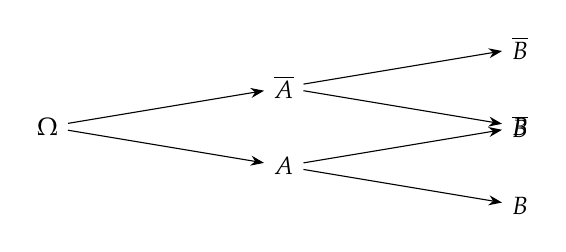
\begin{tikzpicture}[grow=right,level distance=30mm,sibling distance=10mm,every node/.style={font=\small},edge from parent/.style={draw,-{Stealth}}]
\node {$\Omega$} child {node {$A$} child {node {$B$}} child {node {$\overline B$}}} child {node {$\overline A$} child {node {$B$}} child {node {$\overline B$}}};
\end{tikzpicture}\end{center}
    \end{activite}
    \enseignant{$P(E\cap R)=0.35\times0.04=0.014$. $P(R)=0.014+0.65\times0.09=0.0725$. Have students verbalise the piece of data that triggers the choice of method.}

    \begin{traceecrite}We multiply along a path: $P(A\cap B)=P(A)P_A(B)$. We add the mutually exclusive paths that realise the event.\end{traceecrite}

    \begin{exemple}
    Take the data of the investigation and write the solution in order: definition of the objects, property used, exact or approximate calculation, then a sentence giving the answer. The model answer appears in the teacher edition.
    \end{exemple}
    \enseignant{$P(E\cap R)=0.35\times0.04=0.014$. $P(R)=0.014+0.65\times0.09=0.0725$.}

    \begin{exercice}[-- essential]
    \begin{enumerate}\item We know $P(A)=0.45$, $P_A(B)=0.3$ and $P_{\overline A}(B)=0.5$. Construct the tree.\item Calculate $P(A\cap B)$ then $P(B)$.\item Calculate $P_B(A)$ and test independence.\end{enumerate}
    \end{exercice}
    \enseignant{$P(A\cap B)=0.45\times0.3$. Then $P(B)=P(A)P_A(B)+(1-P(A))P_{\overline A}(B)$ and $P_B(A)=\dfrac{P(A\cap B)}{P(B)}$. Compare with $P(A)$.}

    \manuelref{Calao, p. 140, nos.~14--18}
\ExoSession{41}

    \begin{dm}Redo practice exercise 2 with the following data: replace the initial value with $325$ and the rate or ratio with $7$. Write it up in four lines: data, formula, calculation, conclusion.\end{dm}
    \enseignant{The solution depends on the exercise redone. Check above all the consistency of the model, the number of iterations, the rounding and the concluding sentence.}

    \begin{sortie}On a half-sheet: write the main rule of the session, work through a very short example and indicate your confidence level from 1 to 4. Key question(s) of the day: 1, 2 and 3.\end{sortie}

    \ifprof
    \begin{methode}
    \textbf{One-hour plan:} 7 min of fluency; 10 min of pooling and written record; 28 min of essential exercises; 5 min of correction; 3 min of exit ticket.\\
    \textbf{Two-hour plan:} add 20 min of investigation, 20 min of formalisation, a second independent exercise and 10 min of comparative correction.\\
    \textbf{Differentiation:} give struggling students a four-box sheet (data, model, calculation, conclusion). Ask fast students to produce a counterexample, a justification or a second method.
    \end{methode}
    \fi
\sessionheader{42}{18 Mar 2027}{B: 1 h -- C: 2 h}{Independence}{Conditional probability}
\begin{objectifs}\begin{itemize}\item Test independence.\item Compare probabilities.\item Justify a conclusion.\end{itemize}\end{objectifs}
\begin{automatismes}\begin{enumerate}\item Calculate $5\,\%$ of $60$. \rep{$3$}\item Simplify $\dfrac{18}{30}$. \rep{$\dfrac35$}\item What is the sum of the branches leaving a node? \rep{$1$}\item Calculate $0.3\times0.4$. \rep{$0.12$}\item If $P(A)=0.37$, calculate $P(\overline A)$. \rep{$0.63$}\end{enumerate}\end{automatismes}
\begin{prerequis}Reread the last written record and be able to carry out the basic calculations used today. Before the investigation, have the keywords restated: test independence and compare probabilities.\end{prerequis}

\begin{activite}
In a population, $P(A)=0.4$, $P(B)=0.3$ and $P(A\cap B)=0.12$. Test independence in two ways. Then change $P(A\cap B)$ to $0.15$ and start again.

\end{activite}
\enseignant{$0.4\times0.3=0.12$: independence. With $0.15$, the events are no longer independent. Have students verbalise the piece of data that triggers the choice of method.}

\begin{traceecrite}$A$ and $B$ are independent if $P(A\cap B)=P(A)P(B)$, equivalently if $P_A(B)=P(B)$ when $P(A)>0$.\end{traceecrite}

\begin{exemple}
Take the data of the investigation and write the solution in order: definition of the objects, property used, exact or approximate calculation, then a sentence giving the answer. The model answer appears in the teacher edition.
\end{exemple}
\enseignant{$0.4\times0.3=0.12$: independence. With $0.15$, the events are no longer independent.}

\begin{exercice}[-- essential]
\begin{enumerate}\item We know $P(A)=0.20$, $P_A(B)=0.4$ and $P_{\overline A}(B)=0.6$. Construct the tree.\item Calculate $P(A\cap B)$ then $P(B)$.\item Calculate $P_B(A)$ and test independence.\end{enumerate}
\end{exercice}
\enseignant{$P(A\cap B)=0.20\times0.4$. Then $P(B)=P(A)P_A(B)+(1-P(A))P_{\overline A}(B)$ and $P_B(A)=\dfrac{P(A\cap B)}{P(B)}$. Compare with $P(A)$.}

\manuelref{Calao, course pp. 134--137; exercises p. 144, nos.~33--35}
\ExoSession{42}

\begin{dm}Redo practice exercise 3 with the following data: replace the initial value with $330$ and the rate or ratio with $2$. Write it up in four lines: data, formula, calculation, conclusion.\end{dm}
\enseignant{The solution depends on the exercise redone. Check above all the consistency of the model, the number of iterations, the rounding and the concluding sentence.}

\begin{sortie}On a half-sheet: write the main rule of the session, work through a very short example and indicate your confidence level from 1 to 4. Key question(s) of the day: 1 and 2.\end{sortie}

\ifprof
\begin{methode}
\textbf{One-hour plan:} 7 min of fluency; 10 min of pooling and written record; 28 min of essential exercises; 5 min of correction; 3 min of exit ticket.\\
\textbf{Two-hour plan:} add 20 min of investigation, 20 min of formalisation, a second independent exercise and 10 min of comparative correction.\\
\textbf{Differentiation:} give struggling students a four-box sheet (data, model, calculation, conclusion). Ask fast students to produce a counterexample, a justification or a second method.
\end{methode}
\fi
\sessionheader{43}{23 Mar 2027}{B: 2 h -- C: 1 h}{Partition and total probability}{Conditional probability}
    \begin{objectifs}\begin{itemize}\item Recognise a partition.\item Apply total probability.\item Organise the calculation.\end{itemize}\end{objectifs}
    \begin{automatismes}\begin{enumerate}\item Write the multiplier for a $10\,\%$ increase. \rep{$1+\dfrac{10}{100}=1.10$}\item What is the sum of the branches leaving a node? \rep{$1$}\item Calculate $0.4\times0.4$. \rep{$0.16$}\item If $P(A)=0.37$, calculate $P(\overline A)$. \rep{$0.63$}\item Simplify $\dfrac{18}{30}$. \rep{$\dfrac35$}\end{enumerate}\end{automatismes}
    \begin{prerequis}Reread the last written record and be able to carry out the basic calculations used today. Before the investigation, have the keywords restated: recognise a partition and apply total probability.\end{prerequis}

    \begin{activite}
    A factory has three lines A, B, C producing $20\,\%$, $50\,\%$ and $30\,\%$ of the items respectively. Their defect rates are $1\,\%$, $2\,\%$ and $4\,\%$. Calculate the overall defect rate.
    \begin{center}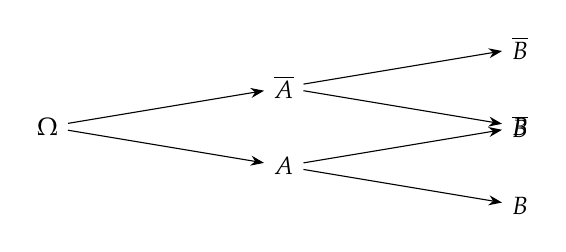
\begin{tikzpicture}[grow=right,level distance=30mm,sibling distance=10mm,every node/.style={font=\small},edge from parent/.style={draw,-{Stealth}}]
\node {$\Omega$} child {node {$A$} child {node {$B$}} child {node {$\overline B$}}} child {node {$\overline A$} child {node {$B$}} child {node {$\overline B$}}};
\end{tikzpicture}\end{center}
    \end{activite}
    \enseignant{$P(D)=0.2\times0.01+0.5\times0.02+0.3\times0.04=0.024$, that is $2.4\,\%$. Have students verbalise the piece of data that triggers the choice of method.}

    \begin{traceecrite}If $(A_i)$ is a partition, $P(B)=\sum_i P(A_i)P_{A_i}(B)$. Each term corresponds to a path leading to $B$.\end{traceecrite}

    \begin{exemple}
    Take the data of the investigation and write the solution in order: definition of the objects, property used, exact or approximate calculation, then a sentence giving the answer. The model answer appears in the teacher edition.
    \end{exemple}
    \enseignant{$P(D)=0.2\times0.01+0.5\times0.02+0.3\times0.04=0.024$, that is $2.4\,\%$.}

    \begin{exercice}[-- essential]
    \begin{enumerate}\item We know $P(A)=0.25$, $P_A(B)=0.5$ and $P_{\overline A}(B)=0.7$. Construct the tree.\item Calculate $P(A\cap B)$ then $P(B)$.\item Calculate $P_B(A)$ and test independence.\end{enumerate}
    \end{exercice}
    \enseignant{$P(A\cap B)=0.25\times0.5$. Then $P(B)=P(A)P_A(B)+(1-P(A))P_{\overline A}(B)$ and $P_B(A)=\dfrac{P(A\cap B)}{P(B)}$. Compare with $P(A)$.}

    \manuelref{Calao, p. 138, nos.~1--5, then p. 142, nos.~22--25}
\ExoSession{43}

    \begin{dm}Redo practice exercise 2 with the following data: replace the initial value with $335$ and the rate or ratio with $3$. Write it up in four lines: data, formula, calculation, conclusion.\end{dm}
    \enseignant{The solution depends on the exercise redone. Check above all the consistency of the model, the number of iterations, the rounding and the concluding sentence.}

    \begin{sortie}On a half-sheet: write the main rule of the session, work through a very short example and indicate your confidence level from 1 to 4. Key question(s) of the day: 1, 2 and 3.\end{sortie}

    \ifprof
    \begin{methode}
    \textbf{One-hour plan:} 7 min of fluency; 10 min of pooling and written record; 28 min of essential exercises; 5 min of correction; 3 min of exit ticket.\\
    \textbf{Two-hour plan:} add 20 min of investigation, 20 min of formalisation, a second independent exercise and 10 min of comparative correction.\\
    \textbf{Differentiation:} give struggling students a four-box sheet (data, model, calculation, conclusion). Ask fast students to produce a counterexample, a justification or a second method.
    \end{methode}
    \fi
\sessionheader{44}{25 Mar 2027}{B: 1 h -- C: 2 h}{Problems in context}{Conditional probability}
\begin{objectifs}\begin{itemize}\item Choose a tree or a table.\item Solve a problem in context.\item Interpret.\end{itemize}\end{objectifs}
\begin{automatismes}\begin{enumerate}\item Simplify $3x+5-x+2$. \rep{$2x+7$}\item Calculate $0.5\times0.4$. \rep{$0.20$}\item If $P(A)=0.37$, calculate $P(\overline A)$. \rep{$0.63$}\item Simplify $\dfrac{18}{30}$. \rep{$\dfrac35$}\item What is the sum of the branches leaving a node? \rep{$1$}\end{enumerate}\end{automatismes}
\begin{prerequis}Reread the last written record and be able to carry out the basic calculations used today. Before the investigation, have the keywords restated: choose a tree or a table and solve a problem in context.\end{prerequis}

\begin{activite}
Turn a table of counts (customers/subscription/cancellation) into a tree, then answer a question in each direction: probability of cancelling given the subscription; probability of having the subscription given the cancellation.

\end{activite}
\enseignant{The first reading uses a row or a branch; the second requires dividing the intersection by the total number of cancellations. Have students verbalise the piece of data that triggers the choice of method.}

\begin{traceecrite}Choosing between a tree and a table: the tree highlights the order of conditioning; the table suits counts and reversed readings well.\end{traceecrite}

\begin{exemple}
Take the data of the investigation and write the solution in order: definition of the objects, property used, exact or approximate calculation, then a sentence giving the answer. The model answer appears in the teacher edition.
\end{exemple}
\enseignant{The first reading uses a row or a branch; the second requires dividing the intersection by the total number of cancellations.}

\begin{exercice}[-- essential]
\begin{enumerate}\item We know $P(A)=0.30$, $P_A(B)=0.6$ and $P_{\overline A}(B)=0.8$. Construct the tree.\item Calculate $P(A\cap B)$ then $P(B)$.\item Calculate $P_B(A)$ and test independence.\end{enumerate}
\end{exercice}
\enseignant{$P(A\cap B)=0.30\times0.6$. Then $P(B)=P(A)P_A(B)+(1-P(A))P_{\overline A}(B)$ and $P_B(A)=\dfrac{P(A\cap B)}{P(B)}$. Compare with $P(A)$.}

\manuelref{Calao, p. 142, nos.~22--25, then p. 144, nos.~30--32}
\ExoSession{44}

\begin{dm}Redo practice exercise 3 with the following data: replace the initial value with $340$ and the rate or ratio with $4$. Write it up in four lines: data, formula, calculation, conclusion.\end{dm}
\enseignant{The solution depends on the exercise redone. Check above all the consistency of the model, the number of iterations, the rounding and the concluding sentence.}

\begin{sortie}On a half-sheet: write the main rule of the session, work through a very short example and indicate your confidence level from 1 to 4. Key question(s) of the day: 1 and 2.\end{sortie}

\ifprof
\begin{methode}
\textbf{One-hour plan:} 7 min of fluency; 10 min of pooling and written record; 28 min of essential exercises; 5 min of correction; 3 min of exit ticket.\\
\textbf{Two-hour plan:} add 20 min of investigation, 20 min of formalisation, a second independent exercise and 10 min of comparative correction.\\
\textbf{Differentiation:} give struggling students a four-box sheet (data, model, calculation, conclusion). Ask fast students to produce a counterexample, a justification or a second method.
\end{methode}
\fi
\sessionheader{45}{30 Mar 2027}{B: 2 h -- C: 1 h}{Mixed practice}{Conditional probability}
    \begin{objectifs}\begin{itemize}\item Calculate a reverse probability.\item Chain total probability and conditioning.\item Check the result.\end{itemize}\end{objectifs}
    \begin{automatismes}\begin{enumerate}\item Calculate $20\,\%$ of $120$. \rep{$24$}\item If $P(A)=0.37$, calculate $P(\overline A)$. \rep{$0.63$}\item Simplify $\dfrac{18}{30}$. \rep{$\dfrac35$}\item What is the sum of the branches leaving a node? \rep{$1$}\item Calculate $0.6\times0.4$. \rep{$0.24$}\end{enumerate}\end{automatismes}
    \begin{prerequis}Reread the last written record and be able to carry out the basic calculations used today. Before the investigation, have the keywords restated: calculate a reverse probability and chain total probability and conditioning.\end{prerequis}

    \begin{activite}
    In the situation of session 43, given that an item is defective, calculate the probability that it comes from line C. Explain why this result is not $30\,\%$.
    \begin{center}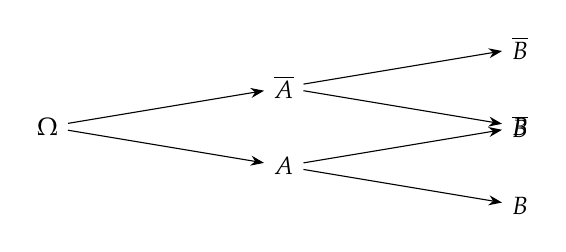
\begin{tikzpicture}[grow=right,level distance=30mm,sibling distance=10mm,every node/.style={font=\small},edge from parent/.style={draw,-{Stealth}}]
\node {$\Omega$} child {node {$A$} child {node {$B$}} child {node {$\overline B$}}} child {node {$\overline A$} child {node {$B$}} child {node {$\overline B$}}};
\end{tikzpicture}\end{center}
    \end{activite}
    \enseignant{$P_D(C)=\dfrac{0.3\times0.04}{0.024}=0.5$. Conditioning changes the distribution because the defect rates differ. Have students verbalise the piece of data that triggers the choice of method.}

    \begin{traceecrite}For a reverse probability, first calculate the total probability of the conditioning event, then use the definition of conditional probability.\end{traceecrite}

    \begin{exemple}
    Take the data of the investigation and write the solution in order: definition of the objects, property used, exact or approximate calculation, then a sentence giving the answer. The model answer appears in the teacher edition.
    \end{exemple}
    \enseignant{$P_D(C)=\dfrac{0.3\times0.04}{0.024}=0.5$. Conditioning changes the distribution because the defect rates differ.}

    \begin{exercice}[-- essential]
    \begin{enumerate}\item We know $P(A)=0.35$, $P_A(B)=0.2$ and $P_{\overline A}(B)=0.4$. Construct the tree.\item Calculate $P(A\cap B)$ then $P(B)$.\item Calculate $P_B(A)$ and test independence.\end{enumerate}
    \end{exercice}
    \enseignant{$P(A\cap B)=0.35\times0.2$. Then $P(B)=P(A)P_A(B)+(1-P(A))P_{\overline A}(B)$ and $P_B(A)=\dfrac{P(A\cap B)}{P(B)}$. Compare with $P(A)$.}

    \manuelref{Calao, pp. 144--146}
\ExoSession{45}

    \begin{dm}Redo practice exercise 2 with the following data: replace the initial value with $345$ and the rate or ratio with $5$. Write it up in four lines: data, formula, calculation, conclusion.\end{dm}
    \enseignant{The solution depends on the exercise redone. Check above all the consistency of the model, the number of iterations, the rounding and the concluding sentence.}

    \begin{sortie}On a half-sheet: write the main rule of the session, work through a very short example and indicate your confidence level from 1 to 4. Key question(s) of the day: 1, 2 and 3.\end{sortie}

    \ifprof
    \begin{methode}
    \textbf{One-hour plan:} 7 min of fluency; 10 min of pooling and written record; 28 min of essential exercises; 5 min of correction; 3 min of exit ticket.\\
    \textbf{Two-hour plan:} add 20 min of investigation, 20 min of formalisation, a second independent exercise and 10 min of comparative correction.\\
    \textbf{Differentiation:} give struggling students a four-box sheet (data, model, calculation, conclusion). Ask fast students to produce a counterexample, a justification or a second method.
    \end{methode}
    \fi
\sessionheader{46}{1 Apr 2027}{B: 1 h -- C: 2 h}{Review and assessment}{Conditional probability}
\begin{objectifs}\begin{itemize}\item Use all the methods.\item Write up with the notation.\item Remedy mistakes.\end{itemize}\end{objectifs}
\begin{automatismes}\begin{enumerate}\item Write the multiplier for a $25\,\%$ increase. \rep{$1+\dfrac{25}{100}=1.25$}\item Simplify $\dfrac{18}{30}$. \rep{$\dfrac35$}\item What is the sum of the branches leaving a node? \rep{$1$}\item Calculate $0.7\times0.4$. \rep{$0.28$}\item If $P(A)=0.37$, calculate $P(\overline A)$. \rep{$0.63$}\end{enumerate}\end{automatismes}
\begin{prerequis}Reread the last written record and be able to carry out the basic calculations used today. Before the investigation, have the keywords restated: use all the methods and write up with the notation.\end{prerequis}

\begin{activite}
Complete a four-station circuit: complete a tree; calculate an intersection; apply the total probability formula; test independence. Each group leaves a written justification for the next group.

\end{activite}
\enseignant{The work produced must contain formulas and interpretations. Mistakes are sorted into: notation, complement, product, sum, reversed conditioning. Have students verbalise the piece of data that triggers the choice of method.}

\begin{traceecrite}Always name the events, complete all the branches, write the formula before calculating and interpret the final probability.\end{traceecrite}

\begin{exemple}
Take the data of the investigation and write the solution in order: definition of the objects, property used, exact or approximate calculation, then a sentence giving the answer. The model answer appears in the teacher edition.
\end{exemple}
\enseignant{The work produced must contain formulas and interpretations. Mistakes are sorted into: notation, complement, product, sum, reversed conditioning.}

\begin{exercice}[-- essential]
\begin{enumerate}\item We know $P(A)=0.40$, $P_A(B)=0.3$ and $P_{\overline A}(B)=0.5$. Construct the tree.\item Calculate $P(A\cap B)$ then $P(B)$.\item Calculate $P_B(A)$ and test independence.\end{enumerate}
\end{exercice}
\enseignant{$P(A\cap B)=0.40\times0.3$. Then $P(B)=P(A)P_A(B)+(1-P(A))P_{\overline A}(B)$ and $P_B(A)=\dfrac{P(A\cap B)}{P(B)}$. Compare with $P(A)$.}

\manuelref{Calao, pp. 146--147}
\ExoSession{46}

\begin{dm}Redo practice exercise 3 with the following data: replace the initial value with $350$ and the rate or ratio with $6$. Write it up in four lines: data, formula, calculation, conclusion.\end{dm}
\enseignant{The solution depends on the exercise redone. Check above all the consistency of the model, the number of iterations, the rounding and the concluding sentence.}

\begin{sortie}On a half-sheet: write the main rule of the session, work through a very short example and indicate your confidence level from 1 to 4. Key question(s) of the day: 1 and 2.\end{sortie}

\ifprof
\begin{methode}
\textbf{One-hour plan:} 7 min of fluency; 10 min of pooling and written record; 28 min of essential exercises; 5 min of correction; 3 min of exit ticket.\\
\textbf{Two-hour plan:} add 20 min of investigation, 20 min of formalisation, a second independent exercise and 10 min of comparative correction.\\
\textbf{Differentiation:} give struggling students a four-box sheet (data, model, calculation, conclusion). Ask fast students to produce a counterexample, a justification or a second method.
\end{methode}
\fi


\chapter{Discrete random variables and the binomial distribution}
\competences{define a distribution, calculate and interpret an expected value, recognise and use a binomial distribution}
\section{Reference notes}
A discrete random variable $X$ assigns a real number to each outcome. Its distribution gives the values $x_i$ and the probabilities $p_i=P(X=x_i)$, with $p_i\geq0$ and $\sum p_i=1$.

\begin{retenir}
The expected value is $E(X)=\sum_i x_ip_i$. It represents the long-run average value when the experiment is repeated under the same conditions; it is not necessarily a value actually taken by $X$.
\end{retenir}

\begin{center}
\begin{tikzpicture}[node distance=9mm and 16mm,every node/.style={draw,circle,inner sep=1.5pt,font=\small}]
\node (a) {1};
\node[below left=of a] (b) {1}; \node[below right=of a] (c) {1};
\node[below left=of b] (d) {1}; \node[below=of a] (e) {2}; \node[below right=of c] (f) {1};
\node[below left=of d] (g) {1}; \node[below left=of e] (h) {3}; \node[below right=of e] (i) {3}; \node[below right=of f] (j) {1};
\draw (a)--(b) (a)--(c) (b)--(d) (b)--(e) (c)--(e) (c)--(f) (d)--(g) (d)--(h) (e)--(h) (e)--(i) (f)--(i) (f)--(j);
\end{tikzpicture}
\end{center}

\begin{retenir}
$X$ follows a binomial distribution $\mathcal B(n,p)$ when $X$ counts the number of successes in $n$ independent Bernoulli trials with the same probability of success $p$. Then
\[
P(X=k)=\binom nk p^k(1-p)^{n-k},\qquad E(X)=np.
\]
\end{retenir}

The binomial coefficient $\binom nk$ counts the number of paths containing exactly $k$ successes among $n$ trials. For $n\leq10$, it can be read from Pascal's triangle.

\begin{center}
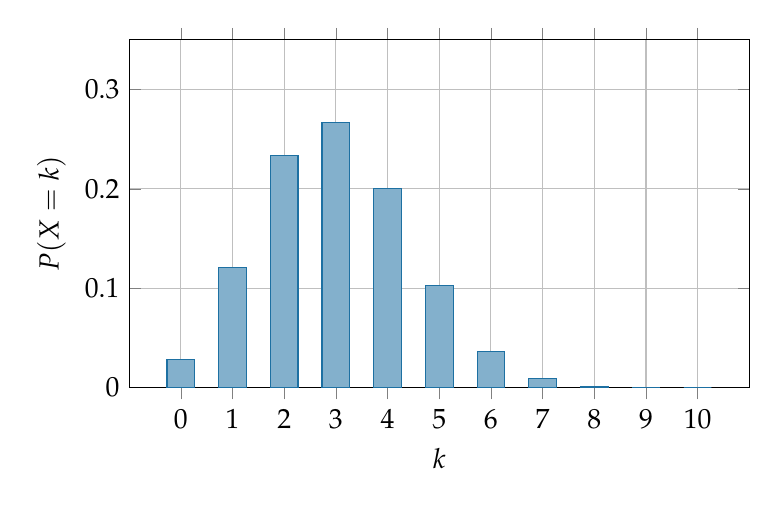
\begin{tikzpicture}
\begin{axis}[ybar,width=.78\textwidth,height=6cm,xlabel={$k$},ylabel={$P(X=k)$},ymin=0,ymax=.35,xtick=data,grid=major]
\addplot[fill=Blue!55,draw=Blue] coordinates {(0,.0282)(1,.1211)(2,.2335)(3,.2668)(4,.2001)(5,.1029)(6,.0368)(7,.0090)(8,.0015)(9,.0002)(10,.0000)};
\end{axis}
\end{tikzpicture}
\end{center}
The diagram approximately represents $\mathcal B(10,0.3)$; its centre is close to $E(X)=3$.

\sessionheader{47}{6 Apr 2027}{B: 2 h -- C: 1 h}{Expected value of a random variable}{Discrete random variables}
\begin{objectifs}\begin{itemize}\item Define a distribution.\item Calculate an expected value.\item Interpret a theoretical average.\end{itemize}\end{objectifs}
\begin{automatismes}\begin{enumerate}\item Simplify $3x+8-x+2$. \rep{$2x+10$}\item Give $E(X)$ for $X\sim\mathcal B(10,0.3)$. \rep{$3$}\item Calculate $\binom52$. \rep{$10$}\item Calculate the expected value of the constant $X$ equal to $8$. \rep{$8$}\item Express $X\geq1$ using a complement. \rep{$1-P(X=0)$}\end{enumerate}\end{automatismes}
\begin{prerequis}Reread the last written record and be able to carry out the basic calculations needed today. Before the investigation, have students rephrase the key words: define a distribution and calculate an expected value.\end{prerequis}

\begin{activite}
A game costs $2$ euros. The gross winnings are $0$, $3$ or $10$ euros with probabilities $0.6$, $0.3$, $0.1$. Construct the distribution of the net gain $X$, calculate $E(X)$ and decide whether the game is favourable to the player.

\end{activite}
\enseignant{$X$ takes the values $-2,1,8$. $E(X)=-1.2+0.3+0.8=-0.1$ euro: the game is unfavourable on average. Have students say aloud which piece of data triggers the choice of method.}

\begin{traceecrite}The distribution of $X$ assigns to each value $x_i$ the probability $p_i$. The expected value $E(X)=\sum x_ip_i$ is a theoretical long-run average.\end{traceecrite}

\begin{exemple}
Take the data from the investigation and write the solution in order: definition of the objects, property used, exact or approximate calculation, then a concluding sentence. The model answer is in the teacher edition.
\end{exemple}
\enseignant{$X$ takes the values $-2,1,8$. $E(X)=-1.2+0.3+0.8=-0.1$ euro: the game is unfavourable on average.}

\begin{exercice}[-- essential]
\begin{enumerate}\item Justify that the number of successes among $8$ independent trials, with $p=0.3$, follows a binomial distribution.\item Calculate $P(X=2)$ and $P(X=0)$.\item Deduce $P(X\geq1)$ and calculate $E(X)$.\end{enumerate}
\end{exercice}
\enseignant{$X\sim\mathcal B(8,0.3)$. $P(X=2)=\binom{8}2 0.3^2 0.7^{6}$, $P(X=0)=0.7^{8}$, $P(X\geq1)=1-P(X=0)$ and $E(X)=\dfrac{24}{10}$.}

\manuelref{Calao, course pp. 154--159; exercises p. 160, no.~1--5}
\CalaoSession{47}

\begin{dm}Redo practice exercise 2 with the following data: replace the initial value by $355$ and the rate or common ratio by $7$. Write it up in four lines: data, formula, calculation, conclusion.\end{dm}
\enseignant{The solution depends on the exercise redone. Check above all the consistency of the model, the number of iterations, the rounding and the concluding sentence.}

\begin{sortie}On a half-sheet: write the main rule of the session, work through a very short example and give a confidence level from 1 to 4. Essential question(s) of the day: 1, 2 and 3.\end{sortie}

\ifprof
\begin{methode}
\textbf{1 h session:} 7 min of fluency; 10 min of pooling and written record; 28 min of essential exercises; 5 min of correction; 3 min of exit ticket.\\
\textbf{2 h session:} add 20 min of investigation, 20 min of formalisation, a second independent exercise and 10 min of comparative correction.\\
\textbf{Differentiation:} give struggling students a four-box sheet (data, model, calculation, conclusion). Ask quick students to produce a counterexample, a justification or a second method.
\end{methode}
\fi
\sessionheader{48}{8 Apr 2027}{B: 1 h -- C: 2 h}{Binomial distribution: recognising a situation}{Discrete random variables}
\begin{objectifs}\begin{itemize}\item Recognise a Bernoulli scheme.\item Identify $n$ and $p$.\item Define $X$.\end{itemize}\end{objectifs}
\begin{automatismes}\begin{enumerate}\item Calculate $5\,\%$ of $180$. \rep{$9$}\item Calculate $\binom52$. \rep{$10$}\item Calculate the expected value of the constant $X$ equal to $9$. \rep{$9$}\item Express $X\geq1$ using a complement. \rep{$1-P(X=0)$}\item Give $E(X)$ for $X\sim\mathcal B(10,0.3)$. \rep{$3$}\end{enumerate}\end{automatismes}
\begin{prerequis}Reread the last written record and be able to carry out the basic calculations needed today. Before the investigation, have students rephrase the key words: recognise a Bernoulli scheme and identify $n$ and $p$.\end{prerequis}

\begin{activite}
A customer accepts an offer with probability $0.25$. An adviser contacts eight customers independently. Define $X$, justify the binomial distribution and identify $n$ and $p$.

\end{activite}
\enseignant{$X$ counts the acceptances; repetition of 8 identical and independent trials, success with probability $0.25$: $X\sim\mathcal B(8,0.25)$. Have students say aloud which piece of data triggers the choice of method.}

\begin{traceecrite}$X\sim\mathcal B(n,p)$ if $X$ counts the successes in $n$ independent trials with the same probability $p$.\end{traceecrite}

\begin{exemple}
Take the data from the investigation and write the solution in order: definition of the objects, property used, exact or approximate calculation, then a concluding sentence. The model answer is in the teacher edition.
\end{exemple}
\enseignant{$X$ counts the acceptances; repetition of 8 identical and independent trials, success with probability $0.25$: $X\sim\mathcal B(8,0.25)$.}

\begin{exercice}[-- essential]
\begin{enumerate}\item Justify that the number of successes among $9$ independent trials, with $p=0.3$, follows a binomial distribution.\item Calculate $P(X=2)$ and $P(X=0)$.\item Deduce $P(X\geq1)$ and calculate $E(X)$.\end{enumerate}
\end{exercice}
\enseignant{$X\sim\mathcal B(9,0.3)$. $P(X=2)=\binom{9}2 0.3^2 0.7^{7}$, $P(X=0)=0.7^{9}$, $P(X\geq1)=1-P(X=0)$ and $E(X)=\dfrac{27}{10}$.}

\manuelref{Calao, course pp. 154--159; exercises p. 160, no.~5, then p. 162, no.~14--20}
\CalaoSession{48}

\begin{dm}Redo practice exercise 3 with the following data: replace the initial value by $360$ and the rate or common ratio by $2$. Write it up in four lines: data, formula, calculation, conclusion.\end{dm}
\enseignant{The solution depends on the exercise redone. Check above all the consistency of the model, the number of iterations, the rounding and the concluding sentence.}

\begin{sortie}On a half-sheet: write the main rule of the session, work through a very short example and give a confidence level from 1 to 4. Essential question(s) of the day: 1 and 2.\end{sortie}

\ifprof
\begin{methode}
\textbf{1 h session:} 7 min of fluency; 10 min of pooling and written record; 28 min of essential exercises; 5 min of correction; 3 min of exit ticket.\\
\textbf{2 h session:} add 20 min of investigation, 20 min of formalisation, a second independent exercise and 10 min of comparative correction.\\
\textbf{Differentiation:} give struggling students a four-box sheet (data, model, calculation, conclusion). Ask quick students to produce a counterexample, a justification or a second method.
\end{methode}
\fi
\sessionheader{49}{27 Apr 2027}{B: 2 h -- C: 1 h}{Pascal's triangle and binomial coefficients}{Discrete random variables}
\begin{objectifs}\begin{itemize}\item Build Pascal's triangle.\item Read $\binom nk$.\item Interpret a coefficient.\end{itemize}\end{objectifs}
\begin{automatismes}\begin{enumerate}\item Write the multiplier for an increase of $10\,\%$. \rep{$1+\dfrac{10}{100}=1.10$}\item Calculate the expected value of the constant $X$ equal to $3$. \rep{$3$}\item Express $X\geq1$ using a complement. \rep{$1-P(X=0)$}\item Give $E(X)$ for $X\sim\mathcal B(10,0.3)$. \rep{$3$}\item Calculate $\binom52$. \rep{$10$}\end{enumerate}\end{automatismes}
\begin{prerequis}Reread the last written record and be able to carry out the basic calculations needed today. Before the investigation, have students rephrase the key words: build Pascal's triangle and read $\binom nk$.\end{prerequis}

\begin{activite}
Build rows $n=0$ to $n=6$ of Pascal's triangle. Explain the calculation of the number $15$ in row $6$, then read $\binom62$ and $\binom64$.
\begin{center}\begin{tabular}{*{9}{c}}&&&&1&&&&\\&&&1&&1&&&\\&&1&&2&&1&&\\&1&&3&&3&&1&\\1&&4&&6&&4&&1\end{tabular}\end{center}
\end{activite}
\enseignant{Each interior number is the sum of the two numbers above it. $\binom62=\binom64=15$. Have students say aloud which piece of data triggers the choice of method.}

\begin{traceecrite}Pascal's triangle satisfies $\binom nk=\binom{n-1}{k-1}+\binom{n-1}{k}$. The edges equal $1$.\end{traceecrite}

\begin{exemple}
Take the data from the investigation and write the solution in order: definition of the objects, property used, exact or approximate calculation, then a concluding sentence. The model answer is in the teacher edition.
\end{exemple}
\enseignant{Each interior number is the sum of the two numbers above it. $\binom62=\binom64=15$.}

\begin{exercice}[-- essential]
\begin{enumerate}\item Justify that the number of successes among $10$ independent trials, with $p=0.3$, follows a binomial distribution.\item Calculate $P(X=2)$ and $P(X=0)$.\item Deduce $P(X\geq1)$ and calculate $E(X)$.\end{enumerate}
\end{exercice}
\enseignant{$X\sim\mathcal B(10,0.3)$. $P(X=2)=\binom{10}2 0.3^2 0.7^{8}$, $P(X=0)=0.7^{10}$, $P(X\geq1)=1-P(X=0)$ and $E(X)=\dfrac{30}{10}$.}

\manuelref{Calao, p. 164, no.~24--29, then p. 166, no.~36}
\CalaoSession{49}

\begin{dm}Redo practice exercise 2 with the following data: replace the initial value by $365$ and the rate or common ratio by $3$. Write it up in four lines: data, formula, calculation, conclusion.\end{dm}
\enseignant{The solution depends on the exercise redone. Check above all the consistency of the model, the number of iterations, the rounding and the concluding sentence.}

\begin{sortie}On a half-sheet: write the main rule of the session, work through a very short example and give a confidence level from 1 to 4. Essential question(s) of the day: 1, 2 and 3.\end{sortie}

\ifprof
\begin{methode}
\textbf{1 h session:} 7 min of fluency; 10 min of pooling and written record; 28 min of essential exercises; 5 min of correction; 3 min of exit ticket.\\
\textbf{2 h session:} add 20 min of investigation, 20 min of formalisation, a second independent exercise and 10 min of comparative correction.\\
\textbf{Differentiation:} give struggling students a four-box sheet (data, model, calculation, conclusion). Ask quick students to produce a counterexample, a justification or a second method.
\end{methode}
\fi
\sessionheader{50}{29 Apr 2027}{B: 1 h -- C: 2 h}{Binomial probabilities}{Discrete random variables}
\begin{objectifs}\begin{itemize}\item Calculate $P(X=k)$.\item Translate at least/at most.\item Use the complement.\end{itemize}\end{objectifs}
\begin{automatismes}\begin{enumerate}\item Simplify $3x+4-x+2$. \rep{$2x+6$}\item Express $X\geq1$ using a complement. \rep{$1-P(X=0)$}\item Give $E(X)$ for $X\sim\mathcal B(10,0.3)$. \rep{$3$}\item Calculate $\binom52$. \rep{$10$}\item Calculate the expected value of the constant $X$ equal to $4$. \rep{$4$}\end{enumerate}\end{automatismes}
\begin{prerequis}Reread the last written record and be able to carry out the basic calculations needed today. Before the investigation, have students rephrase the key words: calculate $p(x=k)$ and translate at least/at most.\end{prerequis}

\begin{activite}
For $X\sim\mathcal B(8,0.25)$, calculate $P(X=2)$, $P(X=0)$, then $P(X\geq1)$. Translate each event into a sentence.
\begin{center}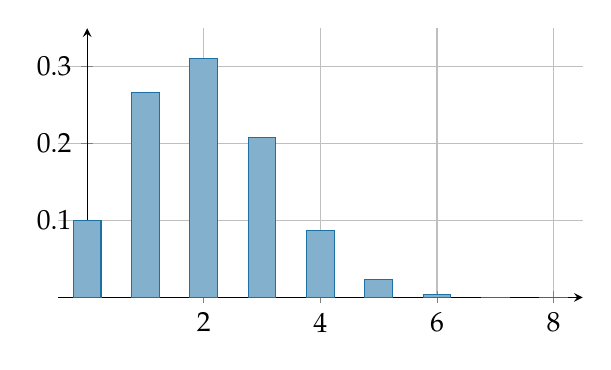
\begin{tikzpicture}\begin{axis}[width=.68\textwidth,height=5cm,axis lines=middle,xmin=-.5,xmax=8.5,ymin=0,ymax=.35,grid=major]\addplot[ybar,fill=Blue!55,draw=Blue] coordinates {(0,.10)(1,.267)(2,.311)(3,.208)(4,.087)(5,.023)(6,.004)(7,.0004)(8,.00002)};\end{axis}\end{tikzpicture}\end{center}
\end{activite}
\enseignant{$P(X=2)=\binom82 0.25^2 0.75^6\approx0.3115$; $P(X=0)=0.75^8\approx0.1001$; $P(X\geq1)\approx0.8999$. Have students say aloud which piece of data triggers the choice of method.}

\begin{traceecrite}If $X\sim\mathcal B(n,p)$, then $P(X=k)=\binom nkp^k(1-p)^{n-k}$. Translate ``at least'', ``at most'' and ``none'' carefully.\end{traceecrite}

\begin{exemple}
Take the data from the investigation and write the solution in order: definition of the objects, property used, exact or approximate calculation, then a concluding sentence. The model answer is in the teacher edition.
\end{exemple}
\enseignant{$P(X=2)=\binom82 0.25^2 0.75^6\approx0.3115$; $P(X=0)=0.75^8\approx0.1001$; $P(X\geq1)\approx0.8999$.}

\begin{exercice}[-- essential]
\begin{enumerate}\item Justify that the number of successes among $6$ independent trials, with $p=0.3$, follows a binomial distribution.\item Calculate $P(X=2)$ and $P(X=0)$.\item Deduce $P(X\geq1)$ and calculate $E(X)$.\end{enumerate}
\end{exercice}
\enseignant{$X\sim\mathcal B(6,0.3)$. $P(X=2)=\binom{6}2 0.3^2 0.7^{4}$, $P(X=0)=0.7^{6}$, $P(X\geq1)=1-P(X=0)$ and $E(X)=\dfrac{18}{10}$.}

\manuelref{Calao, p. 164, no.~24--29, then p. 168, no.~41--45}
\CalaoSession{50}

\begin{dm}Redo practice exercise 3 with the following data: replace the initial value by $370$ and the rate or common ratio by $4$. Write it up in four lines: data, formula, calculation, conclusion.\end{dm}
\enseignant{The solution depends on the exercise redone. Check above all the consistency of the model, the number of iterations, the rounding and the concluding sentence.}

\begin{sortie}On a half-sheet: write the main rule of the session, work through a very short example and give a confidence level from 1 to 4. Essential question(s) of the day: 1 and 2.\end{sortie}

\ifprof
\begin{methode}
\textbf{1 h session:} 7 min of fluency; 10 min of pooling and written record; 28 min of essential exercises; 5 min of correction; 3 min of exit ticket.\\
\textbf{2 h session:} add 20 min of investigation, 20 min of formalisation, a second independent exercise and 10 min of comparative correction.\\
\textbf{Differentiation:} give struggling students a four-box sheet (data, model, calculation, conclusion). Ask quick students to produce a counterexample, a justification or a second method.
\end{methode}
\fi
\sessionheader{51}{4 May 2027}{B: 2 h -- C: 1 h}{Chapter review and test}{Discrete random variables}
\begin{objectifs}\begin{itemize}\item Calculate and interpret $E(X)$.\item Solve a binomial problem.\item Analyse one's mistakes.\end{itemize}\end{objectifs}
\begin{automatismes}\begin{enumerate}\item Calculate $20\,\%$ of $100$. \rep{$20$}\item Give $E(X)$ for $X\sim\mathcal B(10,0.3)$. \rep{$3$}\item Calculate $\binom52$. \rep{$10$}\item Calculate the expected value of the constant $X$ equal to $5$. \rep{$5$}\item Express $X\geq1$ using a complement. \rep{$1-P(X=0)$}\end{enumerate}\end{automatismes}
\begin{prerequis}Reread the last written record and be able to carry out the basic calculations needed today. Before the investigation, have students rephrase the key words: calculate and interpret $e(x)$ and solve a binomial problem.\end{prerequis}

\begin{activite}
A centre receives $120$ groups of $10$ customers, each customer complaining with probability $0.08$. Estimate the average number of complaints per group, then over all the groups. Discuss what the expected value does and does not allow us to predict.

\end{activite}
\enseignant{Per group $E(X)=10\times0.08=0.8$. Over 120 groups, about $96$ complaints on average; this is not a certainty. Have students say aloud which piece of data triggers the choice of method.}

\begin{traceecrite}For $X\sim\mathcal B(n,p)$, $E(X)=np$. The value gives the average number of successes over a large number of series of $n$ trials.\end{traceecrite}

\begin{exemple}
Take the data from the investigation and write the solution in order: definition of the objects, property used, exact or approximate calculation, then a concluding sentence. The model answer is in the teacher edition.
\end{exemple}
\enseignant{Per group $E(X)=10\times0.08=0.8$. Over 120 groups, about $96$ complaints on average; this is not a certainty.}

\begin{exercice}[-- essential]
\begin{enumerate}\item Justify that the number of successes among $7$ independent trials, with $p=0.3$, follows a binomial distribution.\item Calculate $P(X=2)$ and $P(X=0)$.\item Deduce $P(X\geq1)$ and calculate $E(X)$.\end{enumerate}
\end{exercice}
\enseignant{$X\sim\mathcal B(7,0.3)$. $P(X=2)=\binom{7}2 0.3^2 0.7^{5}$, $P(X=0)=0.7^{7}$, $P(X\geq1)=1-P(X=0)$ and $E(X)=\dfrac{21}{10}$.}

\manuelref{Calao, pp. 160--169}
\CalaoSession{51}

\begin{dm}Redo practice exercise 2 with the following data: replace the initial value by $375$ and the rate or common ratio by $5$. Write it up in four lines: data, formula, calculation, conclusion.\end{dm}
\enseignant{The solution depends on the exercise redone. Check above all the consistency of the model, the number of iterations, the rounding and the concluding sentence.}

\begin{sortie}On a half-sheet: write the main rule of the session, work through a very short example and give a confidence level from 1 to 4. Essential question(s) of the day: 1, 2 and 3.\end{sortie}

\ifprof
\begin{methode}
\textbf{1 h session:} 7 min of fluency; 10 min of pooling and written record; 28 min of essential exercises; 5 min of correction; 3 min of exit ticket.\\
\textbf{2 h session:} add 20 min of investigation, 20 min of formalisation, a second independent exercise and 10 min of comparative correction.\\
\textbf{Differentiation:} give struggling students a four-box sheet (data, model, calculation, conclusion). Ask quick students to produce a counterexample, a justification or a second method.
\end{methode}
\fi


\chapter{Revision and consolidation}
\section{Revision strategy}
\begin{retenir}
Effective revision alternates retrieval from memory, explicit correction of mistakes and reuse in a problem. Passively rereading the course is not enough: you must attempt a question without a model, compare your answer, then redo the question after a delay.
\end{retenir}

For each chapter, use the following code: \textbf{V} (mastered), \textbf{O} (shaky), \textbf{R} (to redo). After the diagnosis, work first on an orange or red skill, then check immediately with a similar question.

\begin{center}
\begin{tabularx}{.9\textwidth}{lcccX}
\toprule
Skill & V & O & R & Remedial action \\
\midrule
Choosing a model & $\square$ & $\square$ & $\square$ & Redo a sorting exercise: arithmetic/geometric/exponential.\\
Reading and calculating & $\square$ & $\square$ & $\square$ & Redo the targeted fluency exercises.\\
Writing up and interpreting & $\square$ & $\square$ & $\square$ & Add data, formula, calculation, unit and concluding sentence.\\
\bottomrule
\end{tabularx}
\end{center}

\sessionheader{52}{11 May 2027}{B: 2 h -- C: 1 h}{Diagnosis of what has been learned}{Revision and consolidation}
\begin{objectifs}\begin{itemize}\item Identify what has been learned.\item Classify the mistakes.\item Plan the remediation.\end{itemize}\end{objectifs}
\begin{automatismes}\begin{enumerate}\item Write the multiplier for an increase of $25\,\%$. \rep{$1+\dfrac{25}{100}=1.25$}\item Give the formula for the general term of an arithmetic sequence starting from $u_0$. \rep{$u_n=u_0+nr$}\item Solve $10^x=1000$. \rep{$x=3$}\item Differentiate $x+\dfrac4x$. \rep{$1-\dfrac4{x^2}$}\item State the law of total probability with two branches. \rep{$P(B)=P(A)P_A(B)+P(\overline A)P_{\overline A}(B)$}\end{enumerate}\end{automatismes}
\begin{prerequis}Reread the last written record and be able to carry out the basic calculations needed today. Before the investigation, have students rephrase the key words: identify what has been learned and classify the mistakes.\end{prerequis}

\begin{activite}
Answer 14 questions without the course, two per chapter. Record each mistake in a grid: knowledge, choice of method, calculation, reading, write-up. Then choose two personal priorities.

\end{activite}
\enseignant{The correction expects a profile of mistakes and a plan for catching up, not just an overall mark. Have students say aloud which piece of data triggers the choice of method.}

\begin{traceecrite}The diagnosis is used to choose the remediation: recognise the mistake, recall the useful rule, redo a similar question, then check without help.\end{traceecrite}

\begin{exemple}
Take the data from the investigation and write the solution in order: definition of the objects, property used, exact or approximate calculation, then a concluding sentence. The model answer is in the teacher edition.
\end{exemple}
\enseignant{The correction expects a profile of mistakes and a plan for catching up, not just an overall mark.}

\begin{exercice}[-- essential]
\begin{enumerate}\item Choose between an arithmetic sequence, a geometric sequence and an exponential function in three situations.\item Solve an exponential equation using a logarithm.\item Calculate a probability from a tree, then interpret it.\end{enumerate}
\end{exercice}
\enseignant{Justify each choice by absolute or relative change; check positivity before taking the logarithm; multiply along a path and conclude with a sentence.}

\manuelref{Reactivation of chapters 1 to 7}
\ExoSession{52}

\begin{dm}Redo practice exercise 3 with the following data: replace the initial value by $380$ and the rate or common ratio by $6$. Write it up in four lines: data, formula, calculation, conclusion.\end{dm}
\enseignant{The solution depends on the exercise redone. Check above all the consistency of the model, the number of iterations, the rounding and the concluding sentence.}

\begin{sortie}On a half-sheet: write the main rule of the session, work through a very short example and give a confidence level from 1 to 4. Essential question(s) of the day: 1 and 2.\end{sortie}

\ifprof
\begin{methode}
\textbf{1 h session:} 7 min of fluency; 10 min of pooling and written record; 28 min of essential exercises; 5 min of correction; 3 min of exit ticket.\\
\textbf{2 h session:} add 20 min of investigation, 20 min of formalisation, a second independent exercise and 10 min of comparative correction.\\
\textbf{Differentiation:} give struggling students a four-box sheet (data, model, calculation, conclusion). Ask quick students to produce a counterexample, a justification or a second method.
\end{methode}
\fi
\sessionheader{53}{13 May 2027}{B: 1 h -- C: 2 h}{Reactivation: exponential functions}{Revision and consolidation}
\begin{objectifs}\begin{itemize}\item Reactivate exponential models.\item Solve and interpret.\item Check the units.\end{itemize}\end{objectifs}
\begin{automatismes}\begin{enumerate}\item Simplify $3x+7-x+2$. \rep{$2x+9$}\item Solve $10^x=1000$. \rep{$x=3$}\item Differentiate $x+\dfrac4x$. \rep{$1-\dfrac4{x^2}$}\item State the law of total probability with two branches. \rep{$P(B)=P(A)P_A(B)+P(\overline A)P_{\overline A}(B)$}\item Give the formula for the general term of an arithmetic sequence starting from $u_0$. \rep{$u_n=u_0+nr$}\end{enumerate}\end{automatismes}
\begin{prerequis}Reread the last written record and be able to carry out the basic calculations needed today. Before the investigation, have students rephrase the key words: reactivate exponential models and solve and interpret.\end{prerequis}

\begin{activite}
A value of $18\,000$ increases by $3.5\,\%$ per year. Write the model, calculate the value after eight years and determine when it will exceed $25\,000$.
\begin{center}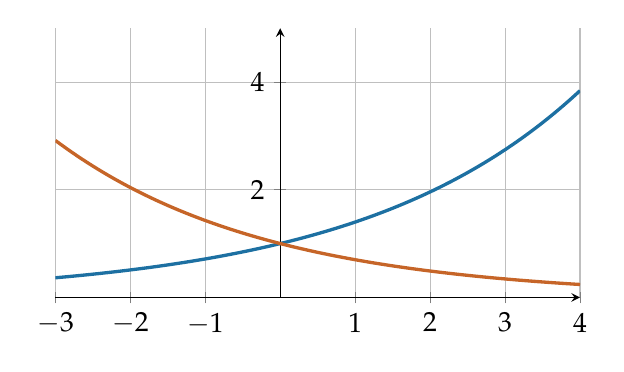
\begin{tikzpicture}\begin{axis}[width=.68\textwidth,height=5cm,axis lines=middle,xmin=-3,xmax=4,ymin=0,ymax=5,grid=major]\addplot[Blue,very thick,samples=100,domain=-3:4]{1.4^x};\addplot[Orange,very thick,samples=100,domain=-3:4]{.7^x};\end{axis}\end{tikzpicture}\end{center}
\end{activite}
\enseignant{$V(t)=18\,000\times1.035^t$, $V(8)\approx23\,703$. The threshold is exceeded from the tenth year onwards. Have students say aloud which piece of data triggers the choice of method.}

\begin{traceecrite}An exponential function models a constant relative change. First identify the initial value and the multiplier.\end{traceecrite}

\begin{exemple}
Take the data from the investigation and write the solution in order: definition of the objects, property used, exact or approximate calculation, then a concluding sentence. The model answer is in the teacher edition.
\end{exemple}
\enseignant{$V(t)=18\,000\times1.035^t$, $V(8)\approx23\,703$. The threshold is exceeded from the tenth year onwards.}

\begin{exercice}[-- essential]
\begin{enumerate}\item Choose between an arithmetic sequence, a geometric sequence and an exponential function in three situations.\item Solve an exponential equation using a logarithm.\item Calculate a probability from a tree, then interpret it.\end{enumerate}
\end{exercice}
\enseignant{Justify each choice by absolute or relative change; check positivity before taking the logarithm; multiply along a path and conclude with a sentence.}

\manuelref{Calao, p. 48, no.~1--8, then p. 54, no.~47--50}
\ExoSession{53}

\begin{dm}Redo practice exercise 2 with the following data: replace the initial value by $385$ and the rate or common ratio by $7$. Write it up in four lines: data, formula, calculation, conclusion.\end{dm}
\enseignant{The solution depends on the exercise redone. Check above all the consistency of the model, the number of iterations, the rounding and the concluding sentence.}

\begin{sortie}On a half-sheet: write the main rule of the session, work through a very short example and give a confidence level from 1 to 4. Essential question(s) of the day: 1, 2 and 3.\end{sortie}

\ifprof
\begin{methode}
\textbf{1 h session:} 7 min of fluency; 10 min of pooling and written record; 28 min of essential exercises; 5 min of correction; 3 min of exit ticket.\\
\textbf{2 h session:} add 20 min of investigation, 20 min of formalisation, a second independent exercise and 10 min of comparative correction.\\
\textbf{Differentiation:} give struggling students a four-box sheet (data, model, calculation, conclusion). Ask quick students to produce a counterexample, a justification or a second method.
\end{methode}
\fi
\sessionheader{54}{18 May 2027}{B: 2 h -- C: 1 h}{Reactivation: common logarithm (base 10)}{Revision and consolidation}
\begin{objectifs}\begin{itemize}\item Reactivate logarithms.\item Solve an equation.\item Check the conditions.\end{itemize}\end{objectifs}
\begin{automatismes}\begin{enumerate}\item Calculate $5\,\%$ of $160$. \rep{$8$}\item Differentiate $x+\dfrac4x$. \rep{$1-\dfrac4{x^2}$}\item State the law of total probability with two branches. \rep{$P(B)=P(A)P_A(B)+P(\overline A)P_{\overline A}(B)$}\item Give the formula for the general term of an arithmetic sequence starting from $u_0$. \rep{$u_n=u_0+nr$}\item Solve $10^x=1000$. \rep{$x=3$}\end{enumerate}\end{automatismes}
\begin{prerequis}Reread the last written record and be able to carry out the basic calculations needed today. Before the investigation, have students rephrase the key words: reactivate logarithms and solve an equation.\end{prerequis}

\begin{activite}
Solve $10^x=340$, $1.06^n=2$ and $1.06^n\geq2$. For each answer, distinguish the real value, the approximate value and the minimum integer index.

\end{activite}
\enseignant{$x\approx2.5315$; $n\approx11.90$; for the integer threshold, $n=12$. Have students say aloud which piece of data triggers the choice of method.}

\begin{traceecrite}The logarithm turns an exponential equation into an equation in the exponent. Conditions: base positive and different from $1$, right-hand side positive.\end{traceecrite}

\begin{exemple}
Take the data from the investigation and write the solution in order: definition of the objects, property used, exact or approximate calculation, then a concluding sentence. The model answer is in the teacher edition.
\end{exemple}
\enseignant{$x\approx2.5315$; $n\approx11.90$; for the integer threshold, $n=12$.}

\begin{exercice}[-- essential]
\begin{enumerate}\item Choose between an arithmetic sequence, a geometric sequence and an exponential function in three situations.\item Solve an exponential equation using a logarithm.\item Calculate a probability from a tree, then interpret it.\end{enumerate}
\end{exercice}
\enseignant{Justify each choice by absolute or relative change; check positivity before taking the logarithm; multiply along a path and conclude with a sentence.}

\manuelref{Calao, p. 70, no.~1--10, then pp. 73--75, no.~30--42}
\ExoSession{54}

\begin{dm}Redo practice exercise 3 with the following data: replace the initial value by $390$ and the rate or common ratio by $2$. Write it up in four lines: data, formula, calculation, conclusion.\end{dm}
\enseignant{The solution depends on the exercise redone. Check above all the consistency of the model, the number of iterations, the rounding and the concluding sentence.}

\begin{sortie}On a half-sheet: write the main rule of the session, work through a very short example and give a confidence level from 1 to 4. Essential question(s) of the day: 1 and 2.\end{sortie}

\ifprof
\begin{methode}
\textbf{1 h session:} 7 min of fluency; 10 min of pooling and written record; 28 min of essential exercises; 5 min of correction; 3 min of exit ticket.\\
\textbf{2 h session:} add 20 min of investigation, 20 min of formalisation, a second independent exercise and 10 min of comparative correction.\\
\textbf{Differentiation:} give struggling students a four-box sheet (data, model, calculation, conclusion). Ask quick students to produce a counterexample, a justification or a second method.
\end{methode}
\fi
\sessionheader{55}{20 May 2027}{B: 1 h -- C: 2 h}{Reactivation: reciprocal function}{Revision and consolidation}
\begin{objectifs}\begin{itemize}\item Reactivate the reciprocal function.\item Carry out a study.\item Sketch and interpret.\end{itemize}\end{objectifs}
\begin{automatismes}\begin{enumerate}\item Write the multiplier for an increase of $10\,\%$. \rep{$1+\dfrac{10}{100}=1.10$}\item State the law of total probability with two branches. \rep{$P(B)=P(A)P_A(B)+P(\overline A)P_{\overline A}(B)$}\item Give the formula for the general term of an arithmetic sequence starting from $u_0$. \rep{$u_n=u_0+nr$}\item Solve $10^x=1000$. \rep{$x=3$}\item Differentiate $x+\dfrac4x$. \rep{$1-\dfrac4{x^2}$}\end{enumerate}\end{automatismes}
\begin{prerequis}Reread the last written record and be able to carry out the basic calculations needed today. Before the investigation, have students rephrase the key words: reactivate the reciprocal function and carry out a study.\end{prerequis}

\begin{activite}
Study $f(x)=x+\dfrac{16}{x}$ on $]0,+\infty[$ and interpret its minimum in an average-cost context. Produce the table of variations and a sketch.
\begin{center}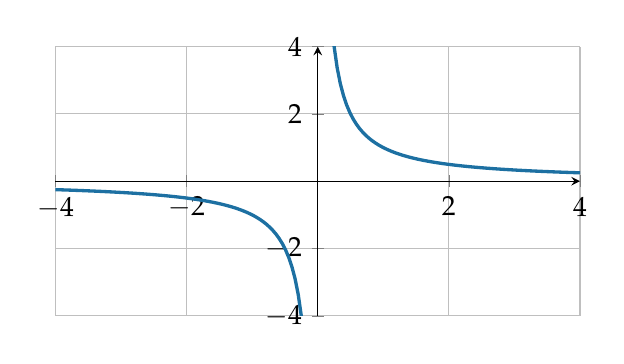
\begin{tikzpicture}\begin{axis}[width=.68\textwidth,height=5cm,axis lines=middle,xmin=-4,xmax=4,ymin=-4,ymax=4,grid=major]\addplot[Blue,very thick,samples=80,domain=-4:-.15]{1/x};\addplot[Blue,very thick,samples=80,domain=.15:4]{1/x};\end{axis}\end{tikzpicture}\end{center}
\end{activite}
\enseignant{$f'(x)=\dfrac{(x-4)(x+4)}{x^2}$; minimum $f(4)=8$. Have students say aloud which piece of data triggers the choice of method.}

\begin{traceecrite}For a function containing $\dfrac1x$, start by excluding $x=0$, then differentiate, factorise and study the sign before the variations.\end{traceecrite}

\begin{exemple}
Take the data from the investigation and write the solution in order: definition of the objects, property used, exact or approximate calculation, then a concluding sentence. The model answer is in the teacher edition.
\end{exemple}
\enseignant{$f'(x)=\dfrac{(x-4)(x+4)}{x^2}$; minimum $f(4)=8$.}

\begin{exercice}[-- essential]
\begin{enumerate}\item Choose between an arithmetic sequence, a geometric sequence and an exponential function in three situations.\item Solve an exponential equation using a logarithm.\item Calculate a probability from a tree, then interpret it.\end{enumerate}
\end{exercice}
\enseignant{Justify each choice by absolute or relative change; check positivity before taking the logarithm; multiply along a path and conclude with a sentence.}

\manuelref{Calao, p. 94, no.~1--9, then p. 96, no.~10--21}
\ExoSession{55}

\begin{dm}Redo practice exercise 2 with the following data: replace the initial value by $395$ and the rate or common ratio by $3$. Write it up in four lines: data, formula, calculation, conclusion.\end{dm}
\enseignant{The solution depends on the exercise redone. Check above all the consistency of the model, the number of iterations, the rounding and the concluding sentence.}

\begin{sortie}On a half-sheet: write the main rule of the session, work through a very short example and give a confidence level from 1 to 4. Essential question(s) of the day: 1, 2 and 3.\end{sortie}

\ifprof
\begin{methode}
\textbf{1 h session:} 7 min of fluency; 10 min of pooling and written record; 28 min of essential exercises; 5 min of correction; 3 min of exit ticket.\\
\textbf{2 h session:} add 20 min of investigation, 20 min of formalisation, a second independent exercise and 10 min of comparative correction.\\
\textbf{Differentiation:} give struggling students a four-box sheet (data, model, calculation, conclusion). Ask quick students to produce a counterexample, a justification or a second method.
\end{methode}
\fi

\appendix
\chapter{Supervised tests}
Two versions are provided for each chapter. The reference structure is: fluency questions worth 6 points, an exercise worth 6 points and a problem worth 8 points.
\section*{Chapter 1 -- Numerical sequences}
\dsheader{1}{A}{Numerical sequences}{model, calculate, reason, communicate}
\begin{exercice}[1 -- Fluency]\points{6}
\begin{enumerate}
\item Give the multiplier associated with an increase of $5\,\%$.
\item Is the sequence $12,17,22,27,\ldots$ arithmetic? Give its common difference.
\item How many terms does $u_4+u_5+\cdots+u_{18}$ contain?
\item If $w_0=80$ and $w_{n+1}=0.9w_n$, calculate $w_2$.
\item Write $1+2+\cdots+20$ using the symbol $\sum$.
\end{enumerate}
\end{exercice}
\begin{exercice}[2 -- Subscriptions]\points{6}
A platform has $120\,000$ subscribers at the start of the year and gains $11\,000$ each month. Let $u_n$ be the number of subscribers, in thousands, after $n$ months.
\begin{enumerate}
\item Show that $(u_n)$ is arithmetic and state its common difference.
\item Express $u_n$ in terms of $n$, then calculate $u_{12}$.
\item Calculate $u_1+\cdots+u_{12}$. Interpret this sum with caution.
\end{enumerate}
\end{exercice}
\begin{exercice}[3 -- Investment and target]\points{8}
An initial capital of $650\,000$ Ar increases by $5\,\%$ per year. Let $C_n$ be the capital after $n$ years.
\begin{enumerate}
\item Write $C_{n+1}$ in terms of $C_n$, then $C_n$ in terms of $n$.
\item Calculate $C_5$, rounded to the nearest ariary.
\item Use a calculator to find the first integer $n$ for which $C_n$ exceeds $1\,000\,000$ Ar.
\item Explain why the model is geometric and not arithmetic.
\end{enumerate}
\end{exercice}
\enseignant{\textbf{Marking scheme.} Ex. 1: 6 points spread over the fluency questions. Ex. 2: 6 points. Ex. 3: 8 points.\\
\textbf{Solution outline.} The multiplier is $1.05$. The first sequence in the fluency questions is arithmetic with common difference $5$; the sum contains $15$ terms; $w_2=64$ and $\sum_{k=1}^{20}k$. For exercise 2, $u_n=120+11n$, so $u_{12}=252$; the requested sum uses $12\dfrac{u_1+u_{12}}2$ and accumulates monthly figures, not a number of distinct people. For exercise 3, $C_n=650\,000\times\left(1+\dfrac{5}{100}\right)^n$; check the threshold with two consecutive values.}

\dsheader{1}{B}{Numerical sequences}{model, calculate, reason, communicate}
\begin{exercice}[1 -- Fluency]\points{6}
\begin{enumerate}
\item Give the multiplier associated with an increase of $4\,\%$.
\item Is the sequence $12,17,22,27,\ldots$ arithmetic? Give its common difference.
\item How many terms does $u_4+u_5+\cdots+u_{18}$ contain?
\item If $w_0=80$ and $w_{n+1}=0.9w_n$, calculate $w_2$.
\item Write $1+2+\cdots+20$ using the symbol $\sum$.
\end{enumerate}
\end{exercice}
\begin{exercice}[2 -- Subscriptions]\points{6}
A platform has $145\,000$ subscribers at the start of the year and gains $9\,000$ each month. Let $u_n$ be the number of subscribers, in thousands, after $n$ months.
\begin{enumerate}
\item Show that $(u_n)$ is arithmetic and state its common difference.
\item Express $u_n$ in terms of $n$, then calculate $u_{12}$.
\item Calculate $u_1+\cdots+u_{12}$. Interpret this sum with caution.
\end{enumerate}
\end{exercice}
\begin{exercice}[3 -- Investment and target]\points{8}
An initial capital of $720\,000$ Ar increases by $4\,\%$ per year. Let $C_n$ be the capital after $n$ years.
\begin{enumerate}
\item Write $C_{n+1}$ in terms of $C_n$, then $C_n$ in terms of $n$.
\item Calculate $C_5$, rounded to the nearest ariary.
\item Use a calculator to find the first integer $n$ for which $C_n$ exceeds $1\,000\,000$ Ar.
\item Explain why the model is geometric and not arithmetic.
\end{enumerate}
\end{exercice}
\enseignant{\textbf{Marking scheme.} Ex. 1: 6 points spread over the fluency questions. Ex. 2: 6 points. Ex. 3: 8 points.\\
\textbf{Solution outline.} The multiplier is $1.04$. The first sequence in the fluency questions is arithmetic with common difference $5$; the sum contains $15$ terms; $w_2=64$ and $\sum_{k=1}^{20}k$. For exercise 2, $u_n=145+9n$, so $u_{12}=253$; the requested sum uses $12\dfrac{u_1+u_{12}}2$ and accumulates monthly figures, not a number of distinct people. For exercise 3, $C_n=720\,000\times\left(1+\dfrac{4}{100}\right)^n$; check the threshold with two consecutive values.}

\section*{Chapter 2 -- Exponential functions}
\dsheader{2}{A}{Exponential functions}{calculate, represent, model, interpret}
\begin{exercice}[1 -- Powers and variations]\points{6}
\begin{enumerate}
\item Simplify $2^4\times2^{-7}$ and $\dfrac{5^{x+3}}{5^x}$.
\item Write $3^{-2}$ as a fraction.
\item Give the direction of variation of $f(x)=1.04^x$ and of $g(x)=-2\times0.75^x$.
\item Explain why $a^x+a^y=a^{x+y}$ is false in general.
\end{enumerate}
\end{exercice}
\begin{exercice}[2 -- Website traffic]\points{6}
At launch, a website receives $2400$ visits per day. Traffic increases by $4\,\%$ per week. It is modelled by $V(t)=2400\times1.04^t$.
\begin{enumerate}
\item Interpret the numbers $2400$ and $1.04$.
\item Calculate $V(8)$, rounded to the nearest unit.
\item Find the first whole number of weeks for which $V(t)>3100$.
\end{enumerate}
\end{exercice}
\begin{exercice}[3 -- Average rate]\points{8}
A company's turnover goes from $82\,000$ to $104000$ euros in four years.
\begin{enumerate}
\item Calculate the overall multiplier.
\item Write the average annual multiplier as a power.
\item Calculate the average annual rate of change (percentage change), rounded to $0.01\,\%$.
\item Explain why the overall rate is not simply divided by four.
\end{enumerate}
\end{exercice}
\enseignant{\textbf{Marking scheme:} $6+6+8$. \textbf{Solution:} $2^4\times2^{-7}=2^{-3}=\dfrac18$, $\dfrac{5^{x+3}}{5^x}=125$, $3^{-2}=\dfrac19$. $f$ is increasing and $g$ is increasing. In the problem, calculate $V(8)$ then test two consecutive integers around the threshold. For the average rate, $q=\left(\dfrac{V_f}{V_i}\right)^{\frac14}$ and $t=q-1$; multipliers multiply.}

\dsheader{2}{B}{Exponential functions}{calculate, represent, model, interpret}
\begin{exercice}[1 -- Powers and variations]\points{6}
\begin{enumerate}
\item Simplify $2^4\times2^{-7}$ and $\dfrac{5^{x+3}}{5^x}$.
\item Write $3^{-2}$ as a fraction.
\item Give the direction of variation of $f(x)=1.03^x$ and of $g(x)=-2\times0.75^x$.
\item Explain why $a^x+a^y=a^{x+y}$ is false in general.
\end{enumerate}
\end{exercice}
\begin{exercice}[2 -- Website traffic]\points{6}
At launch, a website receives $1850$ visits per day. Traffic increases by $3\,\%$ per week. It is modelled by $V(t)=1850\times1.03^t$.
\begin{enumerate}
\item Interpret the numbers $1850$ and $1.03$.
\item Calculate $V(8)$, rounded to the nearest unit.
\item Find the first whole number of weeks for which $V(t)>2250$.
\end{enumerate}
\end{exercice}
\begin{exercice}[3 -- Average rate]\points{8}
A company's turnover goes from $82\,000$ to $98000$ euros in four years.
\begin{enumerate}
\item Calculate the overall multiplier.
\item Write the average annual multiplier as a power.
\item Calculate the average annual rate of change (percentage change), rounded to $0.01\,\%$.
\item Explain why the overall rate is not simply divided by four.
\end{enumerate}
\end{exercice}
\enseignant{\textbf{Marking scheme:} $6+6+8$. \textbf{Solution:} $2^4\times2^{-7}=2^{-3}=\dfrac18$, $\dfrac{5^{x+3}}{5^x}=125$, $3^{-2}=\dfrac19$. $f$ is increasing and $g$ is increasing. In the problem, calculate $V(8)$ then test two consecutive integers around the threshold. For the average rate, $q=\left(\dfrac{V_f}{V_i}\right)^{\frac14}$ and $t=q-1$; multipliers multiply.}

\section*{Chapter 3 -- The common logarithm function}
\dsheader{3}{A}{Common logarithm}{calculate, solve, reason, communicate}
\begin{exercice}[1 -- Knowledge and calculations]\points{6}
\begin{enumerate}
\item Calculate $\log(1000)$, $\log(0.01)$ and $\log(10^{-4})$.
\item For $x,y>0$, expand $\log\!\left(\dfrac{100x^3}{y} \right)$.
\item Solve $10^t=28000$ and give $t$ to the nearest hundredth.
\end{enumerate}
\end{exercice}
\begin{exercice}[2 -- Growth target]\points{6}
A value is multiplied by $1.05$ each year. We look for the time needed for it to double.
\begin{enumerate}
\item Translate the problem into an equation.
\item Solve this equation using the common logarithm (base 10).
\item Give the first whole number of years that reaches or exceeds double.
\item Check with the two relevant consecutive powers.
\end{enumerate}
\end{exercice}
\begin{exercice}[3 -- Sound level]\points{8}
The sound level is $L=10\log\!\left(\dfrac I{I_0}\right)$, in decibels.
\begin{enumerate}
\item Calculate $L$ when $I=10^6I_0$.
\item For $L=84$, express then calculate the ratio $\dfrac I{I_0}$.
\item Compare the intensities corresponding to $84$ dB and $74$ dB.
\end{enumerate}
\end{exercice}
\enseignant{\textbf{Marking scheme:} $6+6+8$. \textbf{Solution:} The usual values are $3,-2,-4$. The expansion gives $2+3\log x-\log y$. $t=\log(28000)$. For the doubling, $x=\dfrac{\log2}{\log(1.05)}$ then take the next integer up and check. $\dfrac I{I_0}=10^{\frac L{10}}$; a difference of $10$ dB corresponds to an intensity multiplied by $10$.}

\dsheader{3}{B}{Common logarithm}{calculate, solve, reason, communicate}
\begin{exercice}[1 -- Knowledge and calculations]\points{6}
\begin{enumerate}
\item Calculate $\log(1000)$, $\log(0.01)$ and $\log(10^{-4})$.
\item For $x,y>0$, expand $\log\!\left(\dfrac{100x^3}{y} \right)$.
\item Solve $10^t=32000$ and give $t$ to the nearest hundredth.
\end{enumerate}
\end{exercice}
\begin{exercice}[2 -- Growth target]\points{6}
A value is multiplied by $1.07$ each year. We look for the time needed for it to double.
\begin{enumerate}
\item Translate the problem into an equation.
\item Solve this equation using the common logarithm (base 10).
\item Give the first whole number of years that reaches or exceeds double.
\item Check with the two relevant consecutive powers.
\end{enumerate}
\end{exercice}
\begin{exercice}[3 -- Sound level]\points{8}
The sound level is $L=10\log\!\left(\dfrac I{I_0}\right)$, in decibels.
\begin{enumerate}
\item Calculate $L$ when $I=10^6I_0$.
\item For $L=78$, express then calculate the ratio $\dfrac I{I_0}$.
\item Compare the intensities corresponding to $78$ dB and $68$ dB.
\end{enumerate}
\end{exercice}
\enseignant{\textbf{Marking scheme:} $6+6+8$. \textbf{Solution:} The usual values are $3,-2,-4$. The expansion gives $2+3\log x-\log y$. $t=\log(32000)$. For the doubling, $x=\dfrac{\log2}{\log(1.07)}$ then take the next integer up and check. $\dfrac I{I_0}=10^{\frac L{10}}$; a difference of $10$ dB corresponds to an intensity multiplied by $10$.}

\section*{Chapter 4 -- The reciprocal function}
\dsheader{4}{A}{Reciprocal function}{calculate, reason, represent, communicate}
\begin{exercice}[1 -- Reciprocal function]\points{6}
Consider $f(x)=2+\dfrac{16}x$.
\begin{enumerate}
\item Give its domain.
\item Calculate its derivative and study its sign.
\item Give its asymptotes and its direction of variation on each interval of the domain.
\end{enumerate}
\end{exercice}
\begin{exercice}[2 -- Sign table]\points{6}
Solve $\dfrac{(x-4)(x+2)}x\geq0$. The table must show the zeros and the excluded value.
\end{exercice}
\begin{exercice}[3 -- Average cost]\points{8}
For $x>0$, an average cost is modelled by $C(x)=x+\dfrac{16}x+12$.
\begin{enumerate}
\item Calculate $C'(x)$ and factorise its numerator.
\item Draw up the variation table of $C$ on $]0,+\infty[$.
\item Find the value of $x$ that minimises the average cost and calculate this minimum.
\item Sketch a consistent graph of the curve.
\end{enumerate}
\end{exercice}
\enseignant{\textbf{Marking scheme:} $6+6+8$. \textbf{Solution:} $D_f=\R\setminus\{0\}$, $f'(x)=-\dfrac{16}{x^2}<0$, asymptotes $x=0$ and $y=2$. For the quotient, order $-2,0,4$ and exclude $0$. For the cost, $C'(x)=1-\dfrac{16}{x^2}=\dfrac{(x-4)(x+4)}{x^2}$; minimum at $x=4$, with value $20$.}

\dsheader{4}{B}{Reciprocal function}{calculate, reason, represent, communicate}
\begin{exercice}[1 -- Reciprocal function]\points{6}
Consider $f(x)=2+\dfrac{9}x$.
\begin{enumerate}
\item Give its domain.
\item Calculate its derivative and study its sign.
\item Give its asymptotes and its direction of variation on each interval of the domain.
\end{enumerate}
\end{exercice}
\begin{exercice}[2 -- Sign table]\points{6}
Solve $\dfrac{(x-3)(x+2)}x\geq0$. The table must show the zeros and the excluded value.
\end{exercice}
\begin{exercice}[3 -- Average cost]\points{8}
For $x>0$, an average cost is modelled by $C(x)=x+\dfrac{9}x+12$.
\begin{enumerate}
\item Calculate $C'(x)$ and factorise its numerator.
\item Draw up the variation table of $C$ on $]0,+\infty[$.
\item Find the value of $x$ that minimises the average cost and calculate this minimum.
\item Sketch a consistent graph of the curve.
\end{enumerate}
\end{exercice}
\enseignant{\textbf{Marking scheme:} $6+6+8$. \textbf{Solution:} $D_f=\R\setminus\{0\}$, $f'(x)=-\dfrac{9}{x^2}<0$, asymptotes $x=0$ and $y=2$. For the quotient, order $-2,0,3$ and exclude $0$. For the cost, $C'(x)=1-\dfrac{9}{x^2}=\dfrac{(x-3)(x+3)}{x^2}$; minimum at $x=3$, with value $18$.}

\section*{Chapter 5 -- Statistics with two quantitative variables}
\dsheader{5}{A}{Two-variable statistics}{represent, model, calculate, interpret}
\begin{exercice}[1 -- Constructing and describing]\points{6}
We observe the pairs $(1;8)$, $(2;11)$, $(3;13)$, $(4;17)$, $(5;19)$ and $(6;23)$.
\begin{enumerate}
\item Draw the scatter plot on a correctly labelled coordinate system.
\item Calculate the coordinates of the mean point.
\item Describe the trend and the spread without concluding that there is causality.
\end{enumerate}
\end{exercice}
\begin{exercice}[2 -- Using a linear regression]\points{6}
A linear regression line is $y=3.2x+12$, established for $x\in[2,15]$.
\begin{enumerate}
\item Estimate $y$ for $x=10$ and characterise the estimate.
\item Estimate $x$ when $y=60$.
\item Estimate $y$ for $x=40$, then explain why this result must be treated with caution.
\end{enumerate}
\end{exercice}
\begin{exercice}[3 -- Change of variable]\points{8}
Let $z=\log(y)$, and the linear regression of $(x,z)$ is $z=0.06x+1.1$.
\begin{enumerate}
\item Express $y$ in terms of $x$.
\item Estimate $y$ for $x=8$.
\item Explain the benefit of the change of variable and one limitation of extrapolation.
\end{enumerate}
\end{exercice}
\enseignant{\textbf{Marking scheme:} $6+6+8$. \textbf{Solution:} Calculate $\bar x$ and $\bar y$ from the six values. With the line, substitute $x$ or solve an equation; $x=10$ is an interpolation and $x=40$ a distant extrapolation. The final model is $y=10^{0.06x+1.1}$.}

\dsheader{5}{B}{Two-variable statistics}{represent, model, calculate, interpret}
\begin{exercice}[1 -- Constructing and describing]\points{6}
We observe the pairs $(1;8)$, $(2;11)$, $(3;13)$, $(4;17)$, $(5;22)$ and $(6;23)$.
\begin{enumerate}
\item Draw the scatter plot on a correctly labelled coordinate system.
\item Calculate the coordinates of the mean point.
\item Describe the trend and the spread without concluding that there is causality.
\end{enumerate}
\end{exercice}
\begin{exercice}[2 -- Using a linear regression]\points{6}
A linear regression line is $y=2.4x+18$, established for $x\in[2,15]$.
\begin{enumerate}
\item Estimate $y$ for $x=10$ and characterise the estimate.
\item Estimate $x$ when $y=60$.
\item Estimate $y$ for $x=40$, then explain why this result must be treated with caution.
\end{enumerate}
\end{exercice}
\begin{exercice}[3 -- Change of variable]\points{8}
Let $z=\log(y)$, and the linear regression of $(x,z)$ is $z=0.06x+1.1$.
\begin{enumerate}
\item Express $y$ in terms of $x$.
\item Estimate $y$ for $x=8$.
\item Explain the benefit of the change of variable and one limitation of extrapolation.
\end{enumerate}
\end{exercice}
\enseignant{\textbf{Marking scheme:} $6+6+8$. \textbf{Solution:} Calculate $\bar x$ and $\bar y$ from the six values. With the line, substitute $x$ or solve an equation; $x=10$ is an interpolation and $x=40$ a distant extrapolation. The final model is $y=10^{0.06x+1.1}$.}

\section*{Chapter 6 -- Conditional probability}
\dsheader{6}{A}{Conditional probability}{model, calculate, reason, interpret}
\begin{exercice}[1 -- Weighted tree]\points{6}
A proportion 0.35 of orders are express. The late-delivery rate is 0.05 among express orders and 0.12 among the others.
\begin{enumerate}
\item Define the events $E$ and $R$, then build the complete weighted tree.
\item Calculate $P(E\cap R)$.
\item Calculate $P(R)$ using the law of total probability.
\item Calculate $P_R(E)$ and interpret.
\end{enumerate}
\end{exercice}
\begin{exercice}[2 -- Independence]\points{6}
In another study, $P(A)=0.4$, $P(B)=0.25$ and $P(A\cap B)=0.10$.
\begin{enumerate}
\item Calculate $P(A)P(B)$.
\item Are the events independent? Justify.
\item Calculate $P_A(B)$ and confirm the conclusion.
\end{enumerate}
\end{exercice}
\begin{exercice}[3 -- Frequency table]\points{8}
Out of $800$ customers, $320$ have a premium card; $96$ premium customers and $72$ non-premium customers cancelled. Build the complete table, then calculate the conditional probability of being premium given that the customer cancelled.
\end{exercice}
\enseignant{\textbf{Marking scheme:} $8+6+6$. \textbf{Solution:} $P(R)=P(E)P_E(R)+P(\overline E)P_{\overline E}(R)$ then $P_R(E)=\dfrac{P(E\cap R)}{P(R)}$. For independence, compare the intersection with the product $0.10$. In the table, there are $168$ cancellations, so $P_R(P)=\dfrac{96}{168}=\dfrac47$.}

\dsheader{6}{B}{Conditional probability}{model, calculate, reason, interpret}
\begin{exercice}[1 -- Weighted tree]\points{6}
A proportion 0.45 of orders are express. The late-delivery rate is 0.08 among express orders and 0.15 among the others.
\begin{enumerate}
\item Define the events $E$ and $R$, then build the complete weighted tree.
\item Calculate $P(E\cap R)$.
\item Calculate $P(R)$ using the law of total probability.
\item Calculate $P_R(E)$ and interpret.
\end{enumerate}
\end{exercice}
\begin{exercice}[2 -- Independence]\points{6}
In another study, $P(A)=0.4$, $P(B)=0.25$ and $P(A\cap B)=0.14$.
\begin{enumerate}
\item Calculate $P(A)P(B)$.
\item Are the events independent? Justify.
\item Calculate $P_A(B)$ and confirm the conclusion.
\end{enumerate}
\end{exercice}
\begin{exercice}[3 -- Frequency table]\points{8}
Out of $800$ customers, $320$ have a premium card; $96$ premium customers and $72$ non-premium customers cancelled. Build the complete table, then calculate the conditional probability of being premium given that the customer cancelled.
\end{exercice}
\enseignant{\textbf{Marking scheme:} $8+6+6$. \textbf{Solution:} $P(R)=P(E)P_E(R)+P(\overline E)P_{\overline E}(R)$ then $P_R(E)=\dfrac{P(E\cap R)}{P(R)}$. For independence, compare the intersection with the product $0.10$. In the table, there are $168$ cancellations, so $P_R(P)=\dfrac{96}{168}=\dfrac47$.}

\section*{Chapter 7 -- Discrete random variables and the binomial distribution}
\dsheader{7}{A}{Random variables and the binomial distribution}{model, calculate, reason, interpret}
\begin{exercice}[1 -- Expected value of a game]\points{6}
A game costs $3$ euros. The gross winnings are $0$, $5$ or $15$ euros with probabilities $0.65$, $0.25$ and $0.10$.
\begin{enumerate}
\item Build the distribution of the net gain $G$.
\item Calculate $E(G)$.
\item Is the game favourable to the player? Interpret without claiming what will happen in a single play.
\end{enumerate}
\end{exercice}
\begin{exercice}[2 -- Binomial distribution]\points{6}
A customer responds favourably with probability $0.30$. An adviser contacts $10$ customers independently. Let $X$ be the number of favourable responses.
\begin{enumerate}
\item Justify the distribution of $X$ and give its parameters.
\item Calculate $P(X=2)$.
\item Calculate $P(X=0)$ then $P(X\geq1)$.
\item Calculate and interpret $E(X)$.
\end{enumerate}
\end{exercice}
\begin{exercice}[3 -- Pascal's triangle]\points{8}
\begin{enumerate}
\item Write row $n=6$ of Pascal's triangle.
\item Read off $\binom62$ and $\binom64$.
\item Explain the role of $\binom nk$ in the binomial formula.
\end{enumerate}
\end{exercice}
\enseignant{\textbf{Marking scheme:} $6+8+6$. \textbf{Solution:} The net gain is $-3,2,12$; $E(G)=-1.95+0.50+1.20=-0.25$ euro. $X\sim\mathcal B(10,0.30)$; apply the formula, use $1-P(X=0)$ for ``at least one'', and $E(X)=np$. Row $n=6$ is $1,6,15,20,15,6,1$.}

\dsheader{7}{B}{Random variables and the binomial distribution}{model, calculate, reason, interpret}
\begin{exercice}[1 -- Expected value of a game]\points{6}
A game costs $3$ euros. The gross winnings are $0$, $5$ or $15$ euros with probabilities $0.65$, $0.25$ and $0.10$.
\begin{enumerate}
\item Build the distribution of the net gain $G$.
\item Calculate $E(G)$.
\item Is the game favourable to the player? Interpret without claiming what will happen in a single play.
\end{enumerate}
\end{exercice}
\begin{exercice}[2 -- Binomial distribution]\points{6}
A customer responds favourably with probability $0.25$. An adviser contacts $8$ customers independently. Let $X$ be the number of favourable responses.
\begin{enumerate}
\item Justify the distribution of $X$ and give its parameters.
\item Calculate $P(X=2)$.
\item Calculate $P(X=0)$ then $P(X\geq1)$.
\item Calculate and interpret $E(X)$.
\end{enumerate}
\end{exercice}
\begin{exercice}[3 -- Pascal's triangle]\points{8}
\begin{enumerate}
\item Write row $n=6$ of Pascal's triangle.
\item Read off $\binom62$ and $\binom64$.
\item Explain the role of $\binom nk$ in the binomial formula.
\end{enumerate}
\end{exercice}
\enseignant{\textbf{Marking scheme:} $6+8+6$. \textbf{Solution:} The net gain is $-3,2,12$; $E(G)=-1.95+0.50+1.20=-0.25$ euro. $X\sim\mathcal B(8,0.25)$; apply the formula, use $1-P(X=0)$ for ``at least one'', and $E(X)=np$. Row $n=6$ is $1,6,15,20,15,6,1$.}

\chapter{Annotated formula sheet}
\begin{longtable}{p{.23\textwidth}p{.33\textwidth}p{.35\textwidth}}
\toprule
Item & Formula & Check to carry out\\
\midrule
Arithmetic sequence & $u_n=u_0+nr$ & Is the first index $0$ or $1$?\\
Arithmetic sum & $N\dfrac{\text{premier}+\text{dernier}}2$ & Count the terms: last index $-$ first index $+1$.\\
Geometric sequence & $u_n=u_0q^n$ & Is $q$ a multiplier rather than a percentage?\\
Geometric sum & $u_0\dfrac{1-q^{n+1}}{1-q}$ & $q\neq1$ and $n+1$ terms.\\
Average rate & $q=Q^{\frac1n}$, $t=q-1$ & Do not divide the overall rate by $n$.\\
Logarithm & $a^x=b\iff x=\dfrac{\log b}{\log a}$ & $a>0$, $a\neq1$, $b>0$.\\
Reciprocal function & $\left(\dfrac1x\right)'=-\dfrac1{x^2}$ & Exclude $x=0$.\\
Linear regression & $y=ax+b$ & Estimate, observed range, unit.\\
Conditioning & $P_A(B)=\dfrac{P(A\cap B)}{P(A)}$ & $P(A)>0$ and order of the conditioning.\\
Total probability & $P(B)=\sum_iP(A_i)P_{A_i}(B)$ & Do the $A_i$ form a partition?\\
Binomial distribution & $P(X=k)=\binom nkp^k(1-p)^{n-k}$ & Independence, same $p$, $0\leq k\leq n$.\\
Binomial expected value & $E(X)=np$ & Interpretation: long-run average.\\
\bottomrule
\end{longtable}

\chapter{Planning table for the 55 sessions}
\small
\begin{longtable}{cclp{.42\textwidth}}
\toprule
No. & Date & Chapter & Topic\\
\midrule\endhead
1 & 15 Sep 2026 & Number Sequences & Arithmetic sequences: recognising and modelling\\
2 & 17 Sep 2026 & Number Sequences & Arithmetic sequences: the general term\\
3 & 22 Sep 2026 & Number Sequences & Sum of the terms of an arithmetic sequence\\
4 & 24 Sep 2026 & Number Sequences & Geometric sequences: recognising and modelling\\
5 & 29 Sep 2026 & Number Sequences & Geometric sequences: general term and sum\\
6 & 1 Oct 2026 & Number Sequences & Review and formative test\\
7 & 6 Oct 2026 & Exponential Functions & Definition and direction of variation of $a^x$\\
8 & 8 Oct 2026 & Exponential Functions & Powers and algebraic properties\\
9 & 13 Oct 2026 & Exponential Functions & Functions $x\mapsto k a^x$: variations and graph\\
10 & 15 Oct 2026 & Exponential Functions & Average rate of change\\
11 & 3 Nov 2026 & Exponential Functions & Reading graphical representations\\
12 & 5 Nov 2026 & Exponential Functions & Simple exponential equations\\
13 & 10 Nov 2026 & Exponential Functions & Modelling with an exponential function\\
14 & 12 Nov 2026 & Exponential Functions & Chapter review and test\\
15 & 17 Nov 2026 & Common logarithm function & Definition of the common logarithm\\
16 & 19 Nov 2026 & Common logarithm function & Direction of variation and graph\\
17 & 24 Nov 2026 & Common logarithm function & Algebraic properties\\
18 & 26 Nov 2026 & Common logarithm function & Solving $10^x=b$\\
19 & 1 Dec 2026 & Common logarithm function & Solving $a^x=b$\\
20 & 3 Dec 2026 & Common logarithm function & Equations $x^a=b$ and simple inequalities\\
21 & 8 Dec 2026 & Common logarithm function & Problems in context\\
22 & 10 Dec 2026 & Common logarithm function & Review and test\\
23 & 15 Dec 2026 & Reciprocal (inverse) function & Definition and curve of the reciprocal function\\
24 & 17 Dec 2026 & Reciprocal (inverse) function & Behaviour at the boundaries and asymptotes\\
25 & 5 Jan 2027 & Reciprocal (inverse) function & Derivative and direction of variation\\
26 & 7 Jan 2027 & Reciprocal (inverse) function & Combinations with polynomial functions\\
27 & 12 Jan 2027 & Reciprocal (inverse) function & Sign and factorisation\\
28 & 14 Jan 2027 & Reciprocal (inverse) function & Derivatives of polynomials of degree at most 3\\
29 & 19 Jan 2027 & Reciprocal (inverse) function & Complete study and graph\\
30 & 21 Jan 2027 & Reciprocal (inverse) function & Review and test\\
31 & 26 Jan 2027 & Two-variable statistics & Scatter plot\\
32 & 28 Jan 2027 & Two-variable statistics & Reading and interpreting the scatter plot\\
33 & 2 Feb 2027 & Two-variable statistics & Linear regression\\
34 & 4 Feb 2027 & Two-variable statistics & Interpolation\\
35 & 9 Feb 2027 & Two-variable statistics & Extrapolation\\
36 & 11 Feb 2027 & Two-variable statistics & Change of variable\\
37 & 2 Mar 2027 & Two-variable statistics & Choice of model and fitting\\
38 & 4 Mar 2027 & Two-variable statistics & Review and test\\
39 & 9 Mar 2027 & Conditional probabilities & Conditioning\\
40 & 11 Mar 2027 & Conditional probabilities & Weighted trees\\
41 & 16 Mar 2027 & Conditional probabilities & Product of probabilities along a path\\
42 & 18 Mar 2027 & Conditional probabilities & Independence\\
43 & 23 Mar 2027 & Conditional probabilities & Partition and total probability\\
44 & 25 Mar 2027 & Conditional probabilities & Problems in context\\
45 & 30 Mar 2027 & Conditional probabilities & Mixed practice\\
46 & 1 Apr 2027 & Conditional probabilities & Review and test\\
47 & 6 Apr 2027 & Discrete random variables & Expected value of a random variable\\
48 & 8 Apr 2027 & Discrete random variables & Binomial distribution: recognising a situation\\
49 & 27 Apr 2027 & Discrete random variables & Pascal's triangle and binomial coefficients\\
50 & 29 Apr 2027 & Discrete random variables & Binomial probabilities\\
51 & 4 May 2027 & Discrete random variables & Chapter review and test\\
52 & 11 May 2027 & Revision and consolidation & Diagnosis of what has been learned\\
53 & 13 May 2027 & Revision and consolidation & Reactivation: exponential functions\\
54 & 18 May 2027 & Revision and consolidation & Reactivation: common logarithm (base 10)\\
55 & 20 May 2027 & Revision and consolidation & Reactivation: reciprocal function\\
\bottomrule
\end{longtable}
\normalsize

\chapter{Sources and status of the content}
\begin{itemize}
\item Ministère de l'Éducation nationale, \emph{Programme de mathématiques de terminale technologique}, special BO no.~8 of 25 July 2019.
\item Éduscol, \emph{Programmes et ressources en mathématiques -- voie générale et technologique}, institutional resources consulted in September 2026.
\item \emph{Calao Mathématiques Terminale technologique}, textbook supplied by the user, pp. 18--169 for the seven chapters used. Each statement reproduced is accompanied by its page and number; the teacher edition provides a detailed solution.
\item \emph{Progression Terminale STMG 2026--2027}, document supplied: calendar, alternation of session lengths and order of topics.
\end{itemize}

\end{document}
